\documentclass[twoside]{book}

% Packages required by doxygen
\usepackage{fixltx2e}
\usepackage{calc}
\usepackage{doxygen}
\usepackage[export]{adjustbox} % also loads graphicx
\usepackage{graphicx}
\usepackage[utf8]{inputenc}
\usepackage{makeidx}
\usepackage{multicol}
\usepackage{multirow}
\PassOptionsToPackage{warn}{textcomp}
\usepackage{textcomp}
\usepackage[nointegrals]{wasysym}
\usepackage[table]{xcolor}

% Font selection
\usepackage[T1]{fontenc}
\usepackage[scaled=.90]{helvet}
\usepackage{courier}
\usepackage{amssymb}
\usepackage{sectsty}
\renewcommand{\familydefault}{\sfdefault}
\allsectionsfont{%
  \fontseries{bc}\selectfont%
  \color{darkgray}%
}
\renewcommand{\DoxyLabelFont}{%
  \fontseries{bc}\selectfont%
  \color{darkgray}%
}
\newcommand{\+}{\discretionary{\mbox{\scriptsize$\hookleftarrow$}}{}{}}

% Page & text layout
\usepackage{geometry}
\geometry{%
  a4paper,%
  top=2.5cm,%
  bottom=2.5cm,%
  left=2.5cm,%
  right=2.5cm%
}
\tolerance=750
\hfuzz=15pt
\hbadness=750
\setlength{\emergencystretch}{15pt}
\setlength{\parindent}{0cm}
\setlength{\parskip}{3ex plus 2ex minus 2ex}
\makeatletter
\renewcommand{\paragraph}{%
  \@startsection{paragraph}{4}{0ex}{-1.0ex}{1.0ex}{%
    \normalfont\normalsize\bfseries\SS@parafont%
  }%
}
\renewcommand{\subparagraph}{%
  \@startsection{subparagraph}{5}{0ex}{-1.0ex}{1.0ex}{%
    \normalfont\normalsize\bfseries\SS@subparafont%
  }%
}
\makeatother

% Headers & footers
\usepackage{fancyhdr}
\pagestyle{fancyplain}
\fancyhead[LE]{\fancyplain{}{\bfseries\thepage}}
\fancyhead[CE]{\fancyplain{}{}}
\fancyhead[RE]{\fancyplain{}{\bfseries\leftmark}}
\fancyhead[LO]{\fancyplain{}{\bfseries\rightmark}}
\fancyhead[CO]{\fancyplain{}{}}
\fancyhead[RO]{\fancyplain{}{\bfseries\thepage}}
\fancyfoot[LE]{\fancyplain{}{}}
\fancyfoot[CE]{\fancyplain{}{}}
\fancyfoot[RE]{\fancyplain{}{\bfseries\scriptsize Generated by Doxygen }}
\fancyfoot[LO]{\fancyplain{}{\bfseries\scriptsize Generated by Doxygen }}
\fancyfoot[CO]{\fancyplain{}{}}
\fancyfoot[RO]{\fancyplain{}{}}
\renewcommand{\footrulewidth}{0.4pt}
\renewcommand{\chaptermark}[1]{%
  \markboth{#1}{}%
}
\renewcommand{\sectionmark}[1]{%
  \markright{\thesection\ #1}%
}

% Indices & bibliography
\usepackage{natbib}
\usepackage[titles]{tocloft}
\setcounter{tocdepth}{3}
\setcounter{secnumdepth}{5}
\makeindex

% Hyperlinks (required, but should be loaded last)
\usepackage{ifpdf}
\ifpdf
  \usepackage[pdftex,pagebackref=true]{hyperref}
\else
  \usepackage[ps2pdf,pagebackref=true]{hyperref}
\fi
\hypersetup{%
  colorlinks=true,%
  linkcolor=blue,%
  citecolor=blue,%
  unicode%
}

% Custom commands
\newcommand{\clearemptydoublepage}{%
  \newpage{\pagestyle{empty}\cleardoublepage}%
}

\usepackage{caption}
\captionsetup{labelsep=space,justification=centering,font={bf},singlelinecheck=off,skip=4pt,position=top}

%===== C O N T E N T S =====

\begin{document}

% Titlepage & ToC
\hypersetup{pageanchor=false,
             bookmarksnumbered=true,
             pdfencoding=unicode
            }
\pagenumbering{alph}
\begin{titlepage}
\vspace*{7cm}
\begin{center}%
{\Large El Tóxico }\\
\vspace*{1cm}
{\large Generated by Doxygen 1.8.14}\\
\end{center}
\end{titlepage}
\clearemptydoublepage
\pagenumbering{roman}
\tableofcontents
\clearemptydoublepage
\pagenumbering{arabic}
\hypersetup{pageanchor=true}

%--- Begin generated contents ---
\chapter{T\+MR}
\label{index}\hypertarget{index}{}\label{index_md_README}%
\Hypertarget{index_md_README}%
\href{https://wakatime.com/badge/user/d1ba7a4d-46ef-44e2-b690-b0f9a744bcc7/project/018bf7bd-7efd-4fc0-897a-61dd82d4afb0}{\texttt{ }} \href{https://wakatime.com/badge/user/d1ba7a4d-46ef-44e2-b690-b0f9a744bcc7/project/a3c94e8d-31ed-4410-941f-117db7cdcb11}{\texttt{ }} \href{https://wakatime.com/badge/user/d1ba7a4d-46ef-44e2-b690-b0f9a744bcc7/project/a74132e0-c0c2-4ea7-81d0-21f509fbf73f}{\texttt{ }} \href{https://wakatime.com/badge/user/d1ba7a4d-46ef-44e2-b690-b0f9a744bcc7/project/c9cdaa12-63d4-488b-b679-9d529c04ba20}{\texttt{ }}

\doxysection*{Stable branch.}

On this branch\textquotesingle{}ll be all the fancy code to compile and run, so this branch will not be updated with the lasts algorithms, only with the stable ones.

\doxysection*{Disclaimer.}

Even this repo has the more stable and fancy scripts, algorithms and codes, these aren\textquotesingle{}t the competition version, so the parameters may change, but i\textquotesingle{}ll try to indicate which parameters you must change and pay special attention.

\doxysection*{Hardware Requeriments.}

The hardware where the robot car run, and is designed to run, has a large list of changes, but i\textquotesingle{}ll put here the more actual hardware (stable only, obviously). ~\newline
 So, the current list is the next. ~\newline



\begin{DoxyItemize}
\item Raspberry pi 4 Model B Rev 1.\+4 8GB.
\item Roboclaw 2x30A.
\item Servomotor Hexfly 60Kg.
\item Redcat Racing Lighting Exp Drift (only the chasis).
\item Personalized 3D printed parts.
\end{DoxyItemize}

\doxysection*{Software Requeriments.}

The software requeriments\textquotesingle{}re more complicated to write correctly, because the current OS has a lot of installed packages, currently we haven\textquotesingle{}t a lis from all this packages, configurations or something like that, tat\textquotesingle{}s because I\textquotesingle{}ll write only the main dependences, but you could open a request, discussion or something like that to help me to make more accurate this list. ~\newline



\begin{DoxyItemize}
\item Ubuntu 22.\+04.\+3 LTS
\item Ros2 Iron
\item Open\+Cv 4.\+8.\+1
\end{DoxyItemize}

\doxysection*{Relevant pkgs.}

\doxysection*{Robot history.}

Along the project lifecycle, there are many authors, so I\textquotesingle{}ll try to make a timeline alongside all the project, since the main team to the current team. ~\newline



\begin{DoxyItemize}
\item 2020
\begin{DoxyItemize}
\item The project start on the first months (I know the first commit has June version), the team was\+:
\item \href{https://github.com/Hector290601}{\texttt{ Robles, Héctor}}. (Team leader)
\item \href{https://github.com/Ricardo-Inaqui}{\texttt{ Ruíz, Iñaki}}. (Mechanic deisgner)
\item \href{https://github.com/jrg-sln}{\texttt{ Solano, Jorge}}. (Team responsable)
\end{DoxyItemize}
\item 2021
\begin{DoxyItemize}
\item Ruíz, Iñaki lefted to team.
\item \href{https://github.com/melaniaromero}{\texttt{ Romero, Melania}} (Programmer) joined to team.
\item \href{https://github.com/mnegretev}{\texttt{ Negrete, Marco}} (Technical guide) joined to team
\end{DoxyItemize}
\item 2022
\begin{DoxyItemize}
\item This\textquotesingle{}s the first year which the robot\textquotesingle{}s inscribed to the TMR, but on the remote simulated league, anyway, we won the \href{https://femexrobotica.org/tmr2022/resultados/}{\texttt{ 3rd}} place.
\item Romero, Melania lefted to team due to time issues.
\item Negrete, Marco helped us to join to \href{https://biorobotics.fi-p.unam.mx/es/}{\texttt{ biorobotics lab}} on the \href{https://www.ingenieria.unam.mx/}{\texttt{ Facultad de Ingeniería}}, \href{https://www.unam.mx/}{\texttt{ UNAM}}.
\item \href{https://github.com/danguer3}{\texttt{ Guerrero, Daniel}} (Programmer) helped us and share his ideas with us.
\item \href{https://github.com/OmarRosCar}{\texttt{ Rosario, Omar}} (Mechanical designer) joined the team.
\item Delgado, Emilio (Programmer) joined to team.
\item Marín, Gustavo (Programmer) joined to team.
\end{DoxyItemize}
\item 2023
\begin{DoxyItemize}
\item This\textquotesingle{}s the first year we could run on the phisical tournament, we won the \href{https://femexrobotica.org/tmr2023/resultados/}{\texttt{ 1st}} place.
\end{DoxyItemize}
\item 2024
\begin{DoxyItemize}
\item Delgado, Emilio lefted to team.
\item Marín, Gustavo lefted to team.
\item Guerrero, Daniel lefted to team
\item \href{https://github.com/JAIRVASQUEZTORRES}{\texttt{ Vasquez, Jair}} (Helper) Joined the team.
\end{DoxyItemize}
\end{DoxyItemize}

\doxysection*{Current team.}

The current team\textquotesingle{}s pefrormed by.


\begin{DoxyItemize}
\item \href{https://github.com/mnegretev}{\texttt{ Negrte, Marco}} (Technical guide)
\item \href{https://github.com/Hector290601}{\texttt{ Robles, Héctor}} (Team Leader)
\item \href{https://github.com/jrg-sln}{\texttt{ Solano, Jorge}} (Team responsable)
\end{DoxyItemize}

\doxysection*{Sponsors.}

Currently we don\textquotesingle{}t have more sponsors than de UNAM, but if you want to become a sponsor to this project, you cand sendus an e-\/mail to the next emails.
\begin{DoxyItemize}
\item \href{mailto:pumasautomodelcar@gmail.com}{\texttt{ Offficial Mail ( pumasautomodelcar@gmail.\+com )}}
\item \href{mailto:marco.negrete@ingenieria.unam.edu}{\texttt{ Negrete, Marco (marco.\+negrete@ingenieria.\+unam.\+edu )}}
\item \href{mailto:robletes062901@gmail.com}{\texttt{ Robles, Hector ( robletes062901@gmail.\+com )}}
\item \href{mailto:jorge.solano@ingenieria.unam.edu}{\texttt{ Solano, Jorge ( jorge.\+solano@ingenieria.\+unam.\+edu )}}
\end{DoxyItemize}

Or anyother mail in our github\textquotesingle{}s profiles. You can check our porpouse on the \href{https://docs.google.com/presentation/d/e/2PACX-1vSj9YTXaojkPzcQOfL-8TyMmTMtzJ04-P1fGeStNJMkl2imKWvjCU_sJmCA23A_Dyrqo8bxcCkdcvh5/pub?start=false&loop=false&delayms=5000}{\texttt{ sponsor\textquotesingle{}s presentation}}.

\doxysection*{Team core.}

The team core\textquotesingle{}s performed by.


\begin{DoxyItemize}
\item \href{https://github.com/mnegretev}{\texttt{ Negrte, Marco}} (Technical guide)
\item \href{https://github.com/Hector290601}{\texttt{ Robles, Héctor}} (Team Leader)
\item \href{https://github.com/jrg-sln}{\texttt{ Solano, Jorge}} (Team responsable) 
\end{DoxyItemize}
\chapter{Namespace Index}
\doxysection{Namespace List}
Here is a list of all namespaces with brief descriptions\+:\begin{DoxyCompactList}
\item\contentsline{section}{\mbox{\hyperlink{namespaceblinkers__interface}{blinkers\+\_\+interface}} }{\pageref{namespaceblinkers__interface}}{}
\item\contentsline{section}{\mbox{\hyperlink{namespacecontroller}{controller}} }{\pageref{namespacecontroller}}{}
\item\contentsline{section}{\mbox{\hyperlink{namespacemotor__interface}{motor\+\_\+interface}} }{\pageref{namespacemotor__interface}}{}
\item\contentsline{section}{\mbox{\hyperlink{namespaceoled__interface}{oled\+\_\+interface}} }{\pageref{namespaceoled__interface}}{}
\item\contentsline{section}{\mbox{\hyperlink{namespaceroboclaw__3}{roboclaw\+\_\+3}} }{\pageref{namespaceroboclaw__3}}{}
\item\contentsline{section}{\mbox{\hyperlink{namespaceservo__interface}{servo\+\_\+interface}} }{\pageref{namespaceservo__interface}}{}
\item\contentsline{section}{\mbox{\hyperlink{namespacesetup}{setup}} }{\pageref{namespacesetup}}{}
\item\contentsline{section}{\mbox{\hyperlink{namespacesitecustomize}{sitecustomize}} }{\pageref{namespacesitecustomize}}{}
\item\contentsline{section}{\mbox{\hyperlink{namespacetoxic__hardware_1_1blinkers__interface}{toxic\+\_\+hardware.\+blinkers\+\_\+interface}} }{\pageref{namespacetoxic__hardware_1_1blinkers__interface}}{}
\item\contentsline{section}{\mbox{\hyperlink{namespacetoxic__hardware_1_1controller}{toxic\+\_\+hardware.\+controller}} }{\pageref{namespacetoxic__hardware_1_1controller}}{}
\item\contentsline{section}{\mbox{\hyperlink{namespacetoxic__hardware_1_1motor__interface}{toxic\+\_\+hardware.\+motor\+\_\+interface}} }{\pageref{namespacetoxic__hardware_1_1motor__interface}}{}
\item\contentsline{section}{\mbox{\hyperlink{namespacetoxic__hardware_1_1oled__interface}{toxic\+\_\+hardware.\+oled\+\_\+interface}} }{\pageref{namespacetoxic__hardware_1_1oled__interface}}{}
\item\contentsline{section}{\mbox{\hyperlink{namespacetoxic__hardware_1_1roboclaw__3}{toxic\+\_\+hardware.\+roboclaw\+\_\+3}} }{\pageref{namespacetoxic__hardware_1_1roboclaw__3}}{}
\item\contentsline{section}{\mbox{\hyperlink{namespacetoxic__hardware_1_1servo__interface}{toxic\+\_\+hardware.\+servo\+\_\+interface}} }{\pageref{namespacetoxic__hardware_1_1servo__interface}}{}
\item\contentsline{section}{\mbox{\hyperlink{namespacetoxic__vision_1_1async__kinect__publisher}{toxic\+\_\+vision.\+async\+\_\+kinect\+\_\+publisher}} }{\pageref{namespacetoxic__vision_1_1async__kinect__publisher}}{}
\item\contentsline{section}{\mbox{\hyperlink{namespacetoxic__vision_1_1color__selector}{toxic\+\_\+vision.\+color\+\_\+selector}} }{\pageref{namespacetoxic__vision_1_1color__selector}}{}
\item\contentsline{section}{\mbox{\hyperlink{namespacetoxic__vision_1_1kinect__publisher}{toxic\+\_\+vision.\+kinect\+\_\+publisher}} }{\pageref{namespacetoxic__vision_1_1kinect__publisher}}{}
\item\contentsline{section}{\mbox{\hyperlink{namespacetoxic__vision_1_1kinect__subscriber}{toxic\+\_\+vision.\+kinect\+\_\+subscriber}} }{\pageref{namespacetoxic__vision_1_1kinect__subscriber}}{}
\item\contentsline{section}{\mbox{\hyperlink{namespacetoxic__vision_1_1lane__detector}{toxic\+\_\+vision.\+lane\+\_\+detector}} }{\pageref{namespacetoxic__vision_1_1lane__detector}}{}
\item\contentsline{section}{\mbox{\hyperlink{namespacetoxic__vision_1_1lane__tracker__p}{toxic\+\_\+vision.\+lane\+\_\+tracker\+\_\+p}} }{\pageref{namespacetoxic__vision_1_1lane__tracker__p}}{}
\item\contentsline{section}{\mbox{\hyperlink{namespacetoxic__vision_1_1webcam__pub}{toxic\+\_\+vision.\+webcam\+\_\+pub}} }{\pageref{namespacetoxic__vision_1_1webcam__pub}}{}
\item\contentsline{section}{\mbox{\hyperlink{namespacetoxic__vision_1_1webcam__sub}{toxic\+\_\+vision.\+webcam\+\_\+sub}} }{\pageref{namespacetoxic__vision_1_1webcam__sub}}{}
\item\contentsline{section}{\mbox{\hyperlink{namespacewebcam__pub}{webcam\+\_\+pub}} }{\pageref{namespacewebcam__pub}}{}
\item\contentsline{section}{\mbox{\hyperlink{namespacewebcam__sub}{webcam\+\_\+sub}} }{\pageref{namespacewebcam__sub}}{}
\end{DoxyCompactList}

\chapter{Hierarchical Index}
\doxysection{Class Hierarchy}
This inheritance list is sorted roughly, but not completely, alphabetically\+:\begin{DoxyCompactList}
\item \contentsline{section}{Roboclaw.\+Cmd}{\pageref{classtoxic__hardware_1_1roboclaw__3_1_1Roboclaw_1_1Cmd}}{}
\item \contentsline{section}{Roboclaw}{\pageref{classtoxic__hardware_1_1roboclaw__3_1_1Roboclaw}}{}
\item Node\begin{DoxyCompactList}
\item \contentsline{section}{Blinkers\+Interface}{\pageref{classtoxic__hardware_1_1blinkers__interface_1_1BlinkersInterface}}{}
\item \contentsline{section}{Blinkers\+Interface}{\pageref{classtoxic__hardware_1_1blinkers__interface_1_1BlinkersInterface}}{}
\item \contentsline{section}{Control\+Subscriber}{\pageref{classtoxic__hardware_1_1controller_1_1ControlSubscriber}}{}
\item \contentsline{section}{Control\+Subscriber}{\pageref{classtoxic__hardware_1_1controller_1_1ControlSubscriber}}{}
\item \contentsline{section}{Motor\+Interface}{\pageref{classtoxic__hardware_1_1motor__interface_1_1MotorInterface}}{}
\item \contentsline{section}{Motor\+Interface}{\pageref{classtoxic__hardware_1_1motor__interface_1_1MotorInterface}}{}
\item \contentsline{section}{Oled\+Interface}{\pageref{classtoxic__hardware_1_1oled__interface_1_1OledInterface}}{}
\item \contentsline{section}{Oled\+Interface}{\pageref{classtoxic__hardware_1_1oled__interface_1_1OledInterface}}{}
\item \contentsline{section}{Steering\+Interface}{\pageref{classtoxic__hardware_1_1servo__interface_1_1SteeringInterface}}{}
\item \contentsline{section}{Steering\+Interface}{\pageref{classtoxic__hardware_1_1servo__interface_1_1SteeringInterface}}{}
\item \contentsline{section}{Image\+Publisher}{\pageref{classtoxic__vision_1_1async__kinect__publisher_1_1ImagePublisher}}{}
\item \contentsline{section}{Image\+Subscriber}{\pageref{classtoxic__vision_1_1color__selector_1_1ImageSubscriber}}{}
\item \contentsline{section}{Image\+Publisher}{\pageref{classtoxic__vision_1_1kinect__publisher_1_1ImagePublisher}}{}
\item \contentsline{section}{Image\+Subscriber}{\pageref{classtoxic__vision_1_1kinect__subscriber_1_1ImageSubscriber}}{}
\item \contentsline{section}{Image\+Subscriber}{\pageref{classtoxic__vision_1_1lane__detector_1_1ImageSubscriber}}{}
\item \contentsline{section}{Image\+Subscriber}{\pageref{classtoxic__vision_1_1lane__detector_1_1ImageSubscriber}}{}
\item \contentsline{section}{Image\+Publisher}{\pageref{classtoxic__vision_1_1webcam__pub_1_1ImagePublisher}}{}
\item \contentsline{section}{Image\+Publisher}{\pageref{classtoxic__vision_1_1webcam__pub_1_1ImagePublisher}}{}
\item \contentsline{section}{Image\+Subscriber}{\pageref{classtoxic__vision_1_1webcam__sub_1_1ImageSubscriber}}{}
\item \contentsline{section}{Image\+Subscriber}{\pageref{classtoxic__vision_1_1webcam__sub_1_1ImageSubscriber}}{}
\end{DoxyCompactList}
\end{DoxyCompactList}

\chapter{Class Index}
\doxysection{Class List}
Here are the classes, structs, unions and interfaces with brief descriptions\+:\begin{DoxyCompactList}
\item\contentsline{section}{\mbox{\hyperlink{classtoxic__hardware_1_1blinkers__interface_1_1BlinkersInterface}{Blinkers\+Interface}} }{\pageref{classtoxic__hardware_1_1blinkers__interface_1_1BlinkersInterface}}{}
\item\contentsline{section}{\mbox{\hyperlink{classtoxic__hardware_1_1roboclaw__3_1_1Roboclaw_1_1Cmd}{Roboclaw.\+Cmd}} }{\pageref{classtoxic__hardware_1_1roboclaw__3_1_1Roboclaw_1_1Cmd}}{}
\item\contentsline{section}{\mbox{\hyperlink{classtoxic__vision_1_1lane__tracker__p_1_1ControllerNode}{Controller\+Node}} }{\pageref{classtoxic__vision_1_1lane__tracker__p_1_1ControllerNode}}{}
\item\contentsline{section}{\mbox{\hyperlink{classtoxic__hardware_1_1controller_1_1ControlSubscriber}{Control\+Subscriber}} }{\pageref{classtoxic__hardware_1_1controller_1_1ControlSubscriber}}{}
\item\contentsline{section}{\mbox{\hyperlink{classtoxic__vision_1_1async__kinect__publisher_1_1ImagePublisher}{Image\+Publisher}} }{\pageref{classtoxic__vision_1_1async__kinect__publisher_1_1ImagePublisher}}{}
\item\contentsline{section}{\mbox{\hyperlink{classtoxic__vision_1_1kinect__publisher_1_1ImagePublisher}{Image\+Publisher}} }{\pageref{classtoxic__vision_1_1kinect__publisher_1_1ImagePublisher}}{}
\item\contentsline{section}{\mbox{\hyperlink{classtoxic__vision_1_1webcam__pub_1_1ImagePublisher}{Image\+Publisher}} }{\pageref{classtoxic__vision_1_1webcam__pub_1_1ImagePublisher}}{}
\item\contentsline{section}{\mbox{\hyperlink{classtoxic__vision_1_1color__selector_1_1ImageSubscriber}{Image\+Subscriber}} }{\pageref{classtoxic__vision_1_1color__selector_1_1ImageSubscriber}}{}
\item\contentsline{section}{\mbox{\hyperlink{classtoxic__vision_1_1kinect__subscriber_1_1ImageSubscriber}{Image\+Subscriber}} }{\pageref{classtoxic__vision_1_1kinect__subscriber_1_1ImageSubscriber}}{}
\item\contentsline{section}{\mbox{\hyperlink{classtoxic__vision_1_1lane__detector_1_1ImageSubscriber}{Image\+Subscriber}} }{\pageref{classtoxic__vision_1_1lane__detector_1_1ImageSubscriber}}{}
\item\contentsline{section}{\mbox{\hyperlink{classtoxic__vision_1_1webcam__sub_1_1ImageSubscriber}{Image\+Subscriber}} }{\pageref{classtoxic__vision_1_1webcam__sub_1_1ImageSubscriber}}{}
\item\contentsline{section}{\mbox{\hyperlink{classtoxic__hardware_1_1motor__interface_1_1MotorInterface}{Motor\+Interface}} }{\pageref{classtoxic__hardware_1_1motor__interface_1_1MotorInterface}}{}
\item\contentsline{section}{\mbox{\hyperlink{classtoxic__hardware_1_1oled__interface_1_1OledInterface}{Oled\+Interface}} }{\pageref{classtoxic__hardware_1_1oled__interface_1_1OledInterface}}{}
\item\contentsline{section}{\mbox{\hyperlink{classtoxic__hardware_1_1roboclaw__3_1_1Roboclaw}{Roboclaw}} }{\pageref{classtoxic__hardware_1_1roboclaw__3_1_1Roboclaw}}{}
\item\contentsline{section}{\mbox{\hyperlink{classtoxic__hardware_1_1servo__interface_1_1SteeringInterface}{Steering\+Interface}} }{\pageref{classtoxic__hardware_1_1servo__interface_1_1SteeringInterface}}{}
\end{DoxyCompactList}

\chapter{File Index}
\doxysection{File List}
Here is a list of all files with brief descriptions\+:\begin{DoxyCompactList}
\item\contentsline{section}{main\+\_\+ws/build/toxic\+\_\+hardware/\mbox{\hyperlink{toxic__hardware_2colcon__command__prefix__setup__py_8sh}{colcon\+\_\+command\+\_\+prefix\+\_\+setup\+\_\+py.\+sh}} }{\pageref{toxic__hardware_2colcon__command__prefix__setup__py_8sh}}{}
\item\contentsline{section}{main\+\_\+ws/build/toxic\+\_\+hardware/build/lib/toxic\+\_\+hardware/\mbox{\hyperlink{automate_8py}{automate.\+py}} }{\pageref{automate_8py}}{}
\item\contentsline{section}{main\+\_\+ws/build/toxic\+\_\+hardware/build/lib/toxic\+\_\+hardware/\mbox{\hyperlink{build_2toxic__hardware_2build_2lib_2toxic__hardware_2blinkers__interface_8py}{blinkers\+\_\+interface.\+py}} }{\pageref{build_2toxic__hardware_2build_2lib_2toxic__hardware_2blinkers__interface_8py}}{}
\item\contentsline{section}{main\+\_\+ws/build/toxic\+\_\+hardware/build/lib/toxic\+\_\+hardware/\mbox{\hyperlink{build_2toxic__hardware_2build_2lib_2toxic__hardware_2controller_8py}{controller.\+py}} }{\pageref{build_2toxic__hardware_2build_2lib_2toxic__hardware_2controller_8py}}{}
\item\contentsline{section}{main\+\_\+ws/build/toxic\+\_\+hardware/build/lib/toxic\+\_\+hardware/\mbox{\hyperlink{gpio__interface_8py}{gpio\+\_\+interface.\+py}} }{\pageref{gpio__interface_8py}}{}
\item\contentsline{section}{main\+\_\+ws/build/toxic\+\_\+hardware/build/lib/toxic\+\_\+hardware/\mbox{\hyperlink{lidar__interface_8py}{lidar\+\_\+interface.\+py}} }{\pageref{lidar__interface_8py}}{}
\item\contentsline{section}{main\+\_\+ws/build/toxic\+\_\+hardware/build/lib/toxic\+\_\+hardware/\mbox{\hyperlink{build_2toxic__hardware_2build_2lib_2toxic__hardware_2motor__interface_8py}{motor\+\_\+interface.\+py}} }{\pageref{build_2toxic__hardware_2build_2lib_2toxic__hardware_2motor__interface_8py}}{}
\item\contentsline{section}{main\+\_\+ws/build/toxic\+\_\+hardware/build/lib/toxic\+\_\+hardware/\mbox{\hyperlink{toxic__hardware_2build_2lib_2toxic__hardware_2obstacle__detector_8py}{obstacle\+\_\+detector.\+py}} }{\pageref{toxic__hardware_2build_2lib_2toxic__hardware_2obstacle__detector_8py}}{}
\item\contentsline{section}{main\+\_\+ws/build/toxic\+\_\+hardware/build/lib/toxic\+\_\+hardware/\mbox{\hyperlink{build_2toxic__hardware_2build_2lib_2toxic__hardware_2oled__interface_8py}{oled\+\_\+interface.\+py}} }{\pageref{build_2toxic__hardware_2build_2lib_2toxic__hardware_2oled__interface_8py}}{}
\item\contentsline{section}{main\+\_\+ws/build/toxic\+\_\+hardware/build/lib/toxic\+\_\+hardware/\mbox{\hyperlink{build_2toxic__hardware_2build_2lib_2toxic__hardware_2roboclaw__3_8py}{roboclaw\+\_\+3.\+py}} }{\pageref{build_2toxic__hardware_2build_2lib_2toxic__hardware_2roboclaw__3_8py}}{}
\item\contentsline{section}{main\+\_\+ws/build/toxic\+\_\+hardware/build/lib/toxic\+\_\+hardware/\mbox{\hyperlink{build_2toxic__hardware_2build_2lib_2toxic__hardware_2servo__interface_8py}{servo\+\_\+interface.\+py}} }{\pageref{build_2toxic__hardware_2build_2lib_2toxic__hardware_2servo__interface_8py}}{}
\item\contentsline{section}{main\+\_\+ws/build/toxic\+\_\+hardware/build/lib/toxic\+\_\+hardware/\mbox{\hyperlink{u__sonics_8py}{u\+\_\+sonics.\+py}} }{\pageref{u__sonics_8py}}{}
\item\contentsline{section}{main\+\_\+ws/build/toxic\+\_\+hardware/prefix\+\_\+override/\mbox{\hyperlink{toxic__hardware_2prefix__override_2sitecustomize_8py}{sitecustomize.\+py}} }{\pageref{toxic__hardware_2prefix__override_2sitecustomize_8py}}{}
\item\contentsline{section}{main\+\_\+ws/build/toxic\+\_\+vision/\mbox{\hyperlink{toxic__vision_2colcon__command__prefix__setup__py_8sh}{colcon\+\_\+command\+\_\+prefix\+\_\+setup\+\_\+py.\+sh}} }{\pageref{toxic__vision_2colcon__command__prefix__setup__py_8sh}}{}
\item\contentsline{section}{main\+\_\+ws/build/toxic\+\_\+vision/build/lib/toxic\+\_\+vision/\mbox{\hyperlink{async__kinect__publisher_8py}{async\+\_\+kinect\+\_\+publisher.\+py}} }{\pageref{async__kinect__publisher_8py}}{}
\item\contentsline{section}{main\+\_\+ws/build/toxic\+\_\+vision/build/lib/toxic\+\_\+vision/\mbox{\hyperlink{color__selector_8py}{color\+\_\+selector.\+py}} }{\pageref{color__selector_8py}}{}
\item\contentsline{section}{main\+\_\+ws/build/toxic\+\_\+vision/build/lib/toxic\+\_\+vision/\mbox{\hyperlink{kinect__publisher_8py}{kinect\+\_\+publisher.\+py}} }{\pageref{kinect__publisher_8py}}{}
\item\contentsline{section}{main\+\_\+ws/build/toxic\+\_\+vision/build/lib/toxic\+\_\+vision/\mbox{\hyperlink{kinect__subscriber_8py}{kinect\+\_\+subscriber.\+py}} }{\pageref{kinect__subscriber_8py}}{}
\item\contentsline{section}{main\+\_\+ws/build/toxic\+\_\+vision/build/lib/toxic\+\_\+vision/\mbox{\hyperlink{lane__detector_8py}{lane\+\_\+detector.\+py}} }{\pageref{lane__detector_8py}}{}
\item\contentsline{section}{main\+\_\+ws/build/toxic\+\_\+vision/build/lib/toxic\+\_\+vision/\mbox{\hyperlink{lane__tracker_8py}{lane\+\_\+tracker.\+py}} }{\pageref{lane__tracker_8py}}{}
\item\contentsline{section}{main\+\_\+ws/build/toxic\+\_\+vision/build/lib/toxic\+\_\+vision/\mbox{\hyperlink{lane__tracker__p_8py}{lane\+\_\+tracker\+\_\+p.\+py}} }{\pageref{lane__tracker__p_8py}}{}
\item\contentsline{section}{main\+\_\+ws/build/toxic\+\_\+vision/build/lib/toxic\+\_\+vision/\mbox{\hyperlink{toxic__vision_2build_2lib_2toxic__vision_2obstacle__detector_8py}{obstacle\+\_\+detector.\+py}} }{\pageref{toxic__vision_2build_2lib_2toxic__vision_2obstacle__detector_8py}}{}
\item\contentsline{section}{main\+\_\+ws/build/toxic\+\_\+vision/build/lib/toxic\+\_\+vision/\mbox{\hyperlink{video__recorder_8py}{video\+\_\+recorder.\+py}} }{\pageref{video__recorder_8py}}{}
\item\contentsline{section}{main\+\_\+ws/build/toxic\+\_\+vision/build/lib/toxic\+\_\+vision/\mbox{\hyperlink{build_2toxic__vision_2build_2lib_2toxic__vision_2webcam__pub_8py}{webcam\+\_\+pub.\+py}} }{\pageref{build_2toxic__vision_2build_2lib_2toxic__vision_2webcam__pub_8py}}{}
\item\contentsline{section}{main\+\_\+ws/build/toxic\+\_\+vision/build/lib/toxic\+\_\+vision/\mbox{\hyperlink{build_2toxic__vision_2build_2lib_2toxic__vision_2webcam__sub_8py}{webcam\+\_\+sub.\+py}} }{\pageref{build_2toxic__vision_2build_2lib_2toxic__vision_2webcam__sub_8py}}{}
\item\contentsline{section}{main\+\_\+ws/build/toxic\+\_\+vision/build/lib/toxic\+\_\+vision/\mbox{\hyperlink{webcam__sub__compressed_8py}{webcam\+\_\+sub\+\_\+compressed.\+py}} }{\pageref{webcam__sub__compressed_8py}}{}
\item\contentsline{section}{main\+\_\+ws/build/toxic\+\_\+vision/prefix\+\_\+override/\mbox{\hyperlink{toxic__vision_2prefix__override_2sitecustomize_8py}{sitecustomize.\+py}} }{\pageref{toxic__vision_2prefix__override_2sitecustomize_8py}}{}
\item\contentsline{section}{main\+\_\+ws/src/toxic\+\_\+hardware/\mbox{\hyperlink{toxic__hardware_2setup_8py}{setup.\+py}} }{\pageref{toxic__hardware_2setup_8py}}{}
\item\contentsline{section}{main\+\_\+ws/src/toxic\+\_\+hardware/toxic\+\_\+hardware/\mbox{\hyperlink{src_2toxic__hardware_2toxic__hardware_2blinkers__interface_8py}{blinkers\+\_\+interface.\+py}} }{\pageref{src_2toxic__hardware_2toxic__hardware_2blinkers__interface_8py}}{}
\item\contentsline{section}{main\+\_\+ws/src/toxic\+\_\+hardware/toxic\+\_\+hardware/\mbox{\hyperlink{src_2toxic__hardware_2toxic__hardware_2controller_8py}{controller.\+py}} }{\pageref{src_2toxic__hardware_2toxic__hardware_2controller_8py}}{}
\item\contentsline{section}{main\+\_\+ws/src/toxic\+\_\+hardware/toxic\+\_\+hardware/\mbox{\hyperlink{src_2toxic__hardware_2toxic__hardware_2motor__interface_8py}{motor\+\_\+interface.\+py}} \\*This script creates a susbcriber node to parse a std\+\_\+msgs.\+msg.\+Float64 ROS\textquotesingle{}s message type to a Roboclaw\textquotesingle{}s serial output }{\pageref{src_2toxic__hardware_2toxic__hardware_2motor__interface_8py}}{}
\item\contentsline{section}{main\+\_\+ws/src/toxic\+\_\+hardware/toxic\+\_\+hardware/\mbox{\hyperlink{src_2toxic__hardware_2toxic__hardware_2oled__interface_8py}{oled\+\_\+interface.\+py}} }{\pageref{src_2toxic__hardware_2toxic__hardware_2oled__interface_8py}}{}
\item\contentsline{section}{main\+\_\+ws/src/toxic\+\_\+hardware/toxic\+\_\+hardware/\mbox{\hyperlink{src_2toxic__hardware_2toxic__hardware_2roboclaw__3_8py}{roboclaw\+\_\+3.\+py}} }{\pageref{src_2toxic__hardware_2toxic__hardware_2roboclaw__3_8py}}{}
\item\contentsline{section}{main\+\_\+ws/src/toxic\+\_\+hardware/toxic\+\_\+hardware/\mbox{\hyperlink{src_2toxic__hardware_2toxic__hardware_2servo__interface_8py}{servo\+\_\+interface.\+py}} }{\pageref{src_2toxic__hardware_2toxic__hardware_2servo__interface_8py}}{}
\item\contentsline{section}{main\+\_\+ws/src/toxic\+\_\+vision/\mbox{\hyperlink{toxic__vision_2setup_8py}{setup.\+py}} }{\pageref{toxic__vision_2setup_8py}}{}
\item\contentsline{section}{main\+\_\+ws/src/toxic\+\_\+vision/toxic\+\_\+vision/\mbox{\hyperlink{src_2toxic__vision_2toxic__vision_2webcam__pub_8py}{webcam\+\_\+pub.\+py}} \\*Main image publisher as /raw\+\_\+rgb node }{\pageref{src_2toxic__vision_2toxic__vision_2webcam__pub_8py}}{}
\item\contentsline{section}{main\+\_\+ws/src/toxic\+\_\+vision/toxic\+\_\+vision/\mbox{\hyperlink{src_2toxic__vision_2toxic__vision_2webcam__sub_8py}{webcam\+\_\+sub.\+py}} \\*Very simple image subscriber to /raw\+\_\+rgb node }{\pageref{src_2toxic__vision_2toxic__vision_2webcam__sub_8py}}{}
\end{DoxyCompactList}

\chapter{Namespace Documentation}
\hypertarget{namespacesetup}{}\doxysection{setup Namespace Reference}
\label{namespacesetup}\index{setup@{setup}}
\doxysubsection*{Variables}
\begin{DoxyCompactItemize}
\item 
string \mbox{\hyperlink{namespacesetup_ad184fbcf6c2a41dfeaea25210baf1d7b}{package\+\_\+name}} = \textquotesingle{}toxic\+\_\+hardware\textquotesingle{}
\item 
\mbox{\hyperlink{namespacesetup_ab74e6bf80237ddc4109968cedc58c151}{name}}
\item 
\mbox{\hyperlink{namespacesetup_a4c7a521b8f1a0769c09bfa4a1fca7dab}{version}}
\item 
\mbox{\hyperlink{namespacesetup_a5191bfd75a28371588f75471591d5500}{packages}}
\item 
\mbox{\hyperlink{namespacesetup_ab2a4f143e926c57a50df01bb182a4fd5}{data\+\_\+files}}
\item 
\mbox{\hyperlink{namespacesetup_a047d4e9f7b152e767f7bd459218fe1fd}{install\+\_\+requires}}
\item 
\mbox{\hyperlink{namespacesetup_a270a33302dcfe1b60738df9ebbfb2103}{zip\+\_\+safe}}
\item 
\mbox{\hyperlink{namespacesetup_aed90451693186afcd612a6e3422085c9}{maintainer}}
\item 
\mbox{\hyperlink{namespacesetup_a3fc04e51dfecacd97621c848af907697}{maintainer\+\_\+email}}
\item 
\mbox{\hyperlink{namespacesetup_a2661f439a4a94ffdcd5e47ae1da0bb1d}{description}}
\item 
\mbox{\hyperlink{namespacesetup_a4e659be027e258b72df12349200a263e}{license}}
\item 
\mbox{\hyperlink{namespacesetup_a04f3a03d8b124a11d2008f990fb6335d}{tests\+\_\+require}}
\item 
\mbox{\hyperlink{namespacesetup_a0afb2eb153236846e2dd516c55a0e0dd}{entry\+\_\+points}}
\end{DoxyCompactItemize}


\doxysubsection{Variable Documentation}
\mbox{\Hypertarget{namespacesetup_ab2a4f143e926c57a50df01bb182a4fd5}\label{namespacesetup_ab2a4f143e926c57a50df01bb182a4fd5}} 
\index{setup@{setup}!data\_files@{data\_files}}
\index{data\_files@{data\_files}!setup@{setup}}
\doxysubsubsection{\texorpdfstring{data\_files}{data\_files}}
{\footnotesize\ttfamily data\+\_\+files}

\mbox{\Hypertarget{namespacesetup_a2661f439a4a94ffdcd5e47ae1da0bb1d}\label{namespacesetup_a2661f439a4a94ffdcd5e47ae1da0bb1d}} 
\index{setup@{setup}!description@{description}}
\index{description@{description}!setup@{setup}}
\doxysubsubsection{\texorpdfstring{description}{description}}
{\footnotesize\ttfamily description}

\mbox{\Hypertarget{namespacesetup_a0afb2eb153236846e2dd516c55a0e0dd}\label{namespacesetup_a0afb2eb153236846e2dd516c55a0e0dd}} 
\index{setup@{setup}!entry\_points@{entry\_points}}
\index{entry\_points@{entry\_points}!setup@{setup}}
\doxysubsubsection{\texorpdfstring{entry\_points}{entry\_points}}
{\footnotesize\ttfamily entry\+\_\+points}

\mbox{\Hypertarget{namespacesetup_a047d4e9f7b152e767f7bd459218fe1fd}\label{namespacesetup_a047d4e9f7b152e767f7bd459218fe1fd}} 
\index{setup@{setup}!install\_requires@{install\_requires}}
\index{install\_requires@{install\_requires}!setup@{setup}}
\doxysubsubsection{\texorpdfstring{install\_requires}{install\_requires}}
{\footnotesize\ttfamily install\+\_\+requires}

\mbox{\Hypertarget{namespacesetup_a4e659be027e258b72df12349200a263e}\label{namespacesetup_a4e659be027e258b72df12349200a263e}} 
\index{setup@{setup}!license@{license}}
\index{license@{license}!setup@{setup}}
\doxysubsubsection{\texorpdfstring{license}{license}}
{\footnotesize\ttfamily license}

\mbox{\Hypertarget{namespacesetup_aed90451693186afcd612a6e3422085c9}\label{namespacesetup_aed90451693186afcd612a6e3422085c9}} 
\index{setup@{setup}!maintainer@{maintainer}}
\index{maintainer@{maintainer}!setup@{setup}}
\doxysubsubsection{\texorpdfstring{maintainer}{maintainer}}
{\footnotesize\ttfamily maintainer}

\mbox{\Hypertarget{namespacesetup_a3fc04e51dfecacd97621c848af907697}\label{namespacesetup_a3fc04e51dfecacd97621c848af907697}} 
\index{setup@{setup}!maintainer\_email@{maintainer\_email}}
\index{maintainer\_email@{maintainer\_email}!setup@{setup}}
\doxysubsubsection{\texorpdfstring{maintainer\_email}{maintainer\_email}}
{\footnotesize\ttfamily maintainer\+\_\+email}

\mbox{\Hypertarget{namespacesetup_ab74e6bf80237ddc4109968cedc58c151}\label{namespacesetup_ab74e6bf80237ddc4109968cedc58c151}} 
\index{setup@{setup}!name@{name}}
\index{name@{name}!setup@{setup}}
\doxysubsubsection{\texorpdfstring{name}{name}}
{\footnotesize\ttfamily name}

\mbox{\Hypertarget{namespacesetup_ad184fbcf6c2a41dfeaea25210baf1d7b}\label{namespacesetup_ad184fbcf6c2a41dfeaea25210baf1d7b}} 
\index{setup@{setup}!package\_name@{package\_name}}
\index{package\_name@{package\_name}!setup@{setup}}
\doxysubsubsection{\texorpdfstring{package\_name}{package\_name}}
{\footnotesize\ttfamily string package\+\_\+name = \textquotesingle{}toxic\+\_\+hardware\textquotesingle{}}

\mbox{\Hypertarget{namespacesetup_a5191bfd75a28371588f75471591d5500}\label{namespacesetup_a5191bfd75a28371588f75471591d5500}} 
\index{setup@{setup}!packages@{packages}}
\index{packages@{packages}!setup@{setup}}
\doxysubsubsection{\texorpdfstring{packages}{packages}}
{\footnotesize\ttfamily packages}

\mbox{\Hypertarget{namespacesetup_a04f3a03d8b124a11d2008f990fb6335d}\label{namespacesetup_a04f3a03d8b124a11d2008f990fb6335d}} 
\index{setup@{setup}!tests\_require@{tests\_require}}
\index{tests\_require@{tests\_require}!setup@{setup}}
\doxysubsubsection{\texorpdfstring{tests\_require}{tests\_require}}
{\footnotesize\ttfamily tests\+\_\+require}

\mbox{\Hypertarget{namespacesetup_a4c7a521b8f1a0769c09bfa4a1fca7dab}\label{namespacesetup_a4c7a521b8f1a0769c09bfa4a1fca7dab}} 
\index{setup@{setup}!version@{version}}
\index{version@{version}!setup@{setup}}
\doxysubsubsection{\texorpdfstring{version}{version}}
{\footnotesize\ttfamily version}

\mbox{\Hypertarget{namespacesetup_a270a33302dcfe1b60738df9ebbfb2103}\label{namespacesetup_a270a33302dcfe1b60738df9ebbfb2103}} 
\index{setup@{setup}!zip\_safe@{zip\_safe}}
\index{zip\_safe@{zip\_safe}!setup@{setup}}
\doxysubsubsection{\texorpdfstring{zip\_safe}{zip\_safe}}
{\footnotesize\ttfamily zip\+\_\+safe}


\hypertarget{namespacetoxic__hardware}{}\section{toxic\+\_\+hardware Namespace Reference}
\label{namespacetoxic__hardware}\index{toxic\+\_\+hardware@{toxic\+\_\+hardware}}
\subsection*{Namespaces}
\begin{DoxyCompactItemize}
\item 
 \mbox{\hyperlink{namespacetoxic__hardware_1_1blinkers__interface}{blinkers\+\_\+interface}}
\item 
 \mbox{\hyperlink{namespacetoxic__hardware_1_1controller}{controller}}
\item 
 \mbox{\hyperlink{namespacetoxic__hardware_1_1motor__interface}{motor\+\_\+interface}}
\item 
 \mbox{\hyperlink{namespacetoxic__hardware_1_1oled__interface}{oled\+\_\+interface}}
\item 
 \mbox{\hyperlink{namespacetoxic__hardware_1_1roboclaw__3}{roboclaw\+\_\+3}}
\item 
 \mbox{\hyperlink{namespacetoxic__hardware_1_1servo__interface}{servo\+\_\+interface}}
\end{DoxyCompactItemize}

\hypertarget{namespacetoxic__hardware_1_1blinkers__interface}{}\doxysection{toxic\+\_\+hardware.\+blinkers\+\_\+interface Namespace Reference}
\label{namespacetoxic__hardware_1_1blinkers__interface}\index{toxic\_hardware.blinkers\_interface@{toxic\_hardware.blinkers\_interface}}
\doxysubsection*{Classes}
\begin{DoxyCompactItemize}
\item 
class \mbox{\hyperlink{classtoxic__hardware_1_1blinkers__interface_1_1BlinkersInterface}{Blinkers\+Interface}}
\end{DoxyCompactItemize}
\doxysubsection*{Functions}
\begin{DoxyCompactItemize}
\item 
def \mbox{\hyperlink{namespacetoxic__hardware_1_1blinkers__interface_a205606096f1ce3bb8e412a407bee6b4b}{main}} (args=None)
\end{DoxyCompactItemize}
\doxysubsection*{Variables}
\begin{DoxyCompactItemize}
\item 
\mbox{\hyperlink{namespacetoxic__hardware_1_1blinkers__interface_a6fd15ce64110e98b208bfe7a4ed33f52}{gpio\+\_\+pin}} = lgpio.\+gpiochip\+\_\+open(0)
\end{DoxyCompactItemize}


\doxysubsection{Function Documentation}
\mbox{\Hypertarget{namespacetoxic__hardware_1_1blinkers__interface_a205606096f1ce3bb8e412a407bee6b4b}\label{namespacetoxic__hardware_1_1blinkers__interface_a205606096f1ce3bb8e412a407bee6b4b}} 
\index{toxic\_hardware.blinkers\_interface@{toxic\_hardware.blinkers\_interface}!main@{main}}
\index{main@{main}!toxic\_hardware.blinkers\_interface@{toxic\_hardware.blinkers\_interface}}
\doxysubsubsection{\texorpdfstring{main()}{main()}}
{\footnotesize\ttfamily def toxic\+\_\+hardware.\+blinkers\+\_\+interface.\+main (\begin{DoxyParamCaption}\item[{}]{args = {\ttfamily None} }\end{DoxyParamCaption})}


\begin{DoxyCode}{0}
\DoxyCodeLine{46 \textcolor{keyword}{def }\mbox{\hyperlink{namespaceblinkers__interface_a784e26b491a03b91359ff42cbf66a1a2}{main}}(args=None):}
\DoxyCodeLine{47     rclpy.init(args=args)}
\DoxyCodeLine{48     blinkersInterface = BlinkersInterface()}
\DoxyCodeLine{49     rclpy.spin(blinkersInterface)}
\DoxyCodeLine{50     blinkersInterface.destroy\_node()}
\DoxyCodeLine{51     rclpy.shutdown()}
\DoxyCodeLine{52 }

\end{DoxyCode}


\doxysubsection{Variable Documentation}
\mbox{\Hypertarget{namespacetoxic__hardware_1_1blinkers__interface_a6fd15ce64110e98b208bfe7a4ed33f52}\label{namespacetoxic__hardware_1_1blinkers__interface_a6fd15ce64110e98b208bfe7a4ed33f52}} 
\index{toxic\_hardware.blinkers\_interface@{toxic\_hardware.blinkers\_interface}!gpio\_pin@{gpio\_pin}}
\index{gpio\_pin@{gpio\_pin}!toxic\_hardware.blinkers\_interface@{toxic\_hardware.blinkers\_interface}}
\doxysubsubsection{\texorpdfstring{gpio\_pin}{gpio\_pin}}
{\footnotesize\ttfamily gpio\+\_\+pin = lgpio.\+gpiochip\+\_\+open(0)}


\hypertarget{namespacetoxic__hardware_1_1controller}{}\doxysection{toxic\+\_\+hardware.\+controller Namespace Reference}
\label{namespacetoxic__hardware_1_1controller}\index{toxic\_hardware.controller@{toxic\_hardware.controller}}
\doxysubsection*{Classes}
\begin{DoxyCompactItemize}
\item 
class \mbox{\hyperlink{classtoxic__hardware_1_1controller_1_1ControlSubscriber}{Control\+Subscriber}}
\end{DoxyCompactItemize}
\doxysubsection*{Functions}
\begin{DoxyCompactItemize}
\item 
def \mbox{\hyperlink{namespacetoxic__hardware_1_1controller_aac60e1fb14a23592e007ebec1efc50a4}{main}} (args=None)
\end{DoxyCompactItemize}
\doxysubsection*{Variables}
\begin{DoxyCompactItemize}
\item 
\mbox{\hyperlink{namespacetoxic__hardware_1_1controller_ae6deea6e7d03b5d4db98ea209159e57f}{interface}} = lgpio.\+gpiochip\+\_\+open(0)
\item 
\mbox{\hyperlink{namespacetoxic__hardware_1_1controller_a257386444c3afd4030922ffb828f85fe}{roboclaw}} = \mbox{\hyperlink{classroboclaw__3_1_1Roboclaw}{Roboclaw}}(\char`\"{}/dev/tty\+ACM0\char`\"{}, 115200)
\end{DoxyCompactItemize}


\doxysubsection{Function Documentation}
\mbox{\Hypertarget{namespacetoxic__hardware_1_1controller_aac60e1fb14a23592e007ebec1efc50a4}\label{namespacetoxic__hardware_1_1controller_aac60e1fb14a23592e007ebec1efc50a4}} 
\index{toxic\_hardware.controller@{toxic\_hardware.controller}!main@{main}}
\index{main@{main}!toxic\_hardware.controller@{toxic\_hardware.controller}}
\doxysubsubsection{\texorpdfstring{main()}{main()}}
{\footnotesize\ttfamily def toxic\+\_\+hardware.\+controller.\+main (\begin{DoxyParamCaption}\item[{}]{args = {\ttfamily None} }\end{DoxyParamCaption})}


\begin{DoxyCode}{0}
\DoxyCodeLine{40 \textcolor{keyword}{def }\mbox{\hyperlink{namespacecontroller_abe3b9157dce8796452422deae2a9161f}{main}}(args=None):}
\DoxyCodeLine{41     rclpy.init(args=args)}
\DoxyCodeLine{42     control\_subscriber = ControlSubscriber()}
\DoxyCodeLine{43     rclpy.spin(control\_subscriber)}
\DoxyCodeLine{44     control\_subscriber.destroy\_node()}
\DoxyCodeLine{45     rclpy.shutdown()}
\DoxyCodeLine{46 }

\end{DoxyCode}


\doxysubsection{Variable Documentation}
\mbox{\Hypertarget{namespacetoxic__hardware_1_1controller_ae6deea6e7d03b5d4db98ea209159e57f}\label{namespacetoxic__hardware_1_1controller_ae6deea6e7d03b5d4db98ea209159e57f}} 
\index{toxic\_hardware.controller@{toxic\_hardware.controller}!interface@{interface}}
\index{interface@{interface}!toxic\_hardware.controller@{toxic\_hardware.controller}}
\doxysubsubsection{\texorpdfstring{interface}{interface}}
{\footnotesize\ttfamily interface = lgpio.\+gpiochip\+\_\+open(0)}

\mbox{\Hypertarget{namespacetoxic__hardware_1_1controller_a257386444c3afd4030922ffb828f85fe}\label{namespacetoxic__hardware_1_1controller_a257386444c3afd4030922ffb828f85fe}} 
\index{toxic\_hardware.controller@{toxic\_hardware.controller}!roboclaw@{roboclaw}}
\index{roboclaw@{roboclaw}!toxic\_hardware.controller@{toxic\_hardware.controller}}
\doxysubsubsection{\texorpdfstring{roboclaw}{roboclaw}}
{\footnotesize\ttfamily roboclaw = \mbox{\hyperlink{classroboclaw__3_1_1Roboclaw}{Roboclaw}}(\char`\"{}/dev/tty\+ACM0\char`\"{}, 115200)}


\hypertarget{namespacetoxic__hardware_1_1motor__interface}{}\section{toxic\+\_\+hardware.\+motor\+\_\+interface Namespace Reference}
\label{namespacetoxic__hardware_1_1motor__interface}\index{toxic\+\_\+hardware.\+motor\+\_\+interface@{toxic\+\_\+hardware.\+motor\+\_\+interface}}
\subsection*{Classes}
\begin{DoxyCompactItemize}
\item 
class \mbox{\hyperlink{classtoxic__hardware_1_1motor__interface_1_1MotorInterface}{Motor\+Interface}}
\end{DoxyCompactItemize}
\subsection*{Functions}
\begin{DoxyCompactItemize}
\item 
def \mbox{\hyperlink{namespacetoxic__hardware_1_1motor__interface_a2a214c16e0dd6e2551c72185d306001e}{main}} (args=None)
\end{DoxyCompactItemize}
\subsection*{Variables}
\begin{DoxyCompactItemize}
\item 
\mbox{\hyperlink{namespacetoxic__hardware_1_1motor__interface_a16c7b96fda2822af1075c24bec28e128}{roboclaw}} = \mbox{\hyperlink{classtoxic__hardware_1_1roboclaw__3_1_1Roboclaw}{Roboclaw}}(\char`\"{}/dev/tty\+A\+C\+M0\char`\"{}, 115200)
\end{DoxyCompactItemize}


\subsection{Function Documentation}
\mbox{\Hypertarget{namespacetoxic__hardware_1_1motor__interface_a2a214c16e0dd6e2551c72185d306001e}\label{namespacetoxic__hardware_1_1motor__interface_a2a214c16e0dd6e2551c72185d306001e}} 
\index{toxic\+\_\+hardware\+::motor\+\_\+interface@{toxic\+\_\+hardware\+::motor\+\_\+interface}!main@{main}}
\index{main@{main}!toxic\+\_\+hardware\+::motor\+\_\+interface@{toxic\+\_\+hardware\+::motor\+\_\+interface}}
\subsubsection{\texorpdfstring{main()}{main()}}
{\footnotesize\ttfamily def toxic\+\_\+hardware.\+motor\+\_\+interface.\+main (\begin{DoxyParamCaption}\item[{}]{args = {\ttfamily None} }\end{DoxyParamCaption})}



\subsection{Variable Documentation}
\mbox{\Hypertarget{namespacetoxic__hardware_1_1motor__interface_a16c7b96fda2822af1075c24bec28e128}\label{namespacetoxic__hardware_1_1motor__interface_a16c7b96fda2822af1075c24bec28e128}} 
\index{toxic\+\_\+hardware\+::motor\+\_\+interface@{toxic\+\_\+hardware\+::motor\+\_\+interface}!roboclaw@{roboclaw}}
\index{roboclaw@{roboclaw}!toxic\+\_\+hardware\+::motor\+\_\+interface@{toxic\+\_\+hardware\+::motor\+\_\+interface}}
\subsubsection{\texorpdfstring{roboclaw}{roboclaw}}
{\footnotesize\ttfamily toxic\+\_\+hardware.\+motor\+\_\+interface.\+roboclaw = \mbox{\hyperlink{classtoxic__hardware_1_1roboclaw__3_1_1Roboclaw}{Roboclaw}}(\char`\"{}/dev/tty\+A\+C\+M0\char`\"{}, 115200)}


\hypertarget{namespacetoxic__hardware_1_1oled__interface}{}\doxysection{toxic\+\_\+hardware.\+oled\+\_\+interface Namespace Reference}
\label{namespacetoxic__hardware_1_1oled__interface}\index{toxic\_hardware.oled\_interface@{toxic\_hardware.oled\_interface}}
\doxysubsection*{Classes}
\begin{DoxyCompactItemize}
\item 
class \mbox{\hyperlink{classtoxic__hardware_1_1oled__interface_1_1OledInterface}{Oled\+Interface}}
\end{DoxyCompactItemize}
\doxysubsection*{Functions}
\begin{DoxyCompactItemize}
\item 
def \mbox{\hyperlink{namespacetoxic__hardware_1_1oled__interface_acb5075a1c586e00088ef12d5117d3902}{main}} (args=None)
\end{DoxyCompactItemize}
\doxysubsection*{Variables}
\begin{DoxyCompactItemize}
\item 
\mbox{\hyperlink{namespacetoxic__hardware_1_1oled__interface_a3a9e2efeaf89528d45ac9a55c0aa0592}{RST}} = None
\item 
int \mbox{\hyperlink{namespacetoxic__hardware_1_1oled__interface_a64c09f22bf1aaf06930f11f70d69b426}{DC}} = 23
\item 
int \mbox{\hyperlink{namespacetoxic__hardware_1_1oled__interface_aa08462d1cbc1c0ce2462199881e1515c}{SPI\+\_\+\+PORT}} = 0
\item 
int \mbox{\hyperlink{namespacetoxic__hardware_1_1oled__interface_ae08d18f8f9a415753075d220a1bba561}{SPI\+\_\+\+DEVICE}} = 0
\item 
\mbox{\hyperlink{namespacetoxic__hardware_1_1oled__interface_a4e72583d972515f4f5e30d98ce1eb739}{disp}} = Adafruit\+\_\+\+SSD1306.\+SSD1306\+\_\+128\+\_\+64(rst=\mbox{\hyperlink{namespacetoxic__hardware_1_1oled__interface_a3a9e2efeaf89528d45ac9a55c0aa0592}{RST}})
\item 
\mbox{\hyperlink{namespacetoxic__hardware_1_1oled__interface_a5558ace5433f9aabbf0a0ec059900d94}{width}} = disp.\+width
\item 
\mbox{\hyperlink{namespacetoxic__hardware_1_1oled__interface_a509290c21d570ff479c1b9d9b1fe8810}{height}} = disp.\+height
\item 
\mbox{\hyperlink{namespacetoxic__hardware_1_1oled__interface_a42cb5f5737262947250c709931232c69}{image}} = Image.\+new(\textquotesingle{}1\textquotesingle{}, (\mbox{\hyperlink{namespacetoxic__hardware_1_1oled__interface_a5558ace5433f9aabbf0a0ec059900d94}{width}}, \mbox{\hyperlink{namespacetoxic__hardware_1_1oled__interface_a509290c21d570ff479c1b9d9b1fe8810}{height}}))
\item 
\mbox{\hyperlink{namespacetoxic__hardware_1_1oled__interface_a349ab7af971a4dba55c235814bbc3a9b}{draw}} = Image\+Draw.\+Draw(\mbox{\hyperlink{namespacetoxic__hardware_1_1oled__interface_a42cb5f5737262947250c709931232c69}{image}})
\item 
\mbox{\hyperlink{namespacetoxic__hardware_1_1oled__interface_a8d9e59eab21bcca5dfbf02faabf38f29}{outline}}
\item 
\mbox{\hyperlink{namespacetoxic__hardware_1_1oled__interface_a23b3ecc690a716b53e9d0146b78d5ef2}{fill}}
\item 
int \mbox{\hyperlink{namespacetoxic__hardware_1_1oled__interface_a78dca952886227190969e885fbdd4fb4}{padding}} = -\/2
\item 
int \mbox{\hyperlink{namespacetoxic__hardware_1_1oled__interface_af93f4f37fc2ad9c37af4a715423b110c}{top}} = \mbox{\hyperlink{namespacetoxic__hardware_1_1oled__interface_a78dca952886227190969e885fbdd4fb4}{padding}}
\item 
int \mbox{\hyperlink{namespacetoxic__hardware_1_1oled__interface_a323a7064fba6e15e3e542e34fb19764e}{bottom}} = \mbox{\hyperlink{namespacetoxic__hardware_1_1oled__interface_a509290c21d570ff479c1b9d9b1fe8810}{height}}-\/\mbox{\hyperlink{namespacetoxic__hardware_1_1oled__interface_a78dca952886227190969e885fbdd4fb4}{padding}}
\item 
int \mbox{\hyperlink{namespacetoxic__hardware_1_1oled__interface_a6150e0515f7202e2fb518f7206ed97dc}{x}} = 0
\item 
\mbox{\hyperlink{namespacetoxic__hardware_1_1oled__interface_af18bb9025627467c42857f6b57902a47}{font}} = Image\+Font.\+load\+\_\+default()
\end{DoxyCompactItemize}


\doxysubsection{Function Documentation}
\mbox{\Hypertarget{namespacetoxic__hardware_1_1oled__interface_acb5075a1c586e00088ef12d5117d3902}\label{namespacetoxic__hardware_1_1oled__interface_acb5075a1c586e00088ef12d5117d3902}} 
\index{toxic\_hardware.oled\_interface@{toxic\_hardware.oled\_interface}!main@{main}}
\index{main@{main}!toxic\_hardware.oled\_interface@{toxic\_hardware.oled\_interface}}
\doxysubsubsection{\texorpdfstring{main()}{main()}}
{\footnotesize\ttfamily def main (\begin{DoxyParamCaption}\item[{}]{args = {\ttfamily None} }\end{DoxyParamCaption})}


\begin{DoxyCode}{0}
\DoxyCodeLine{56 \textcolor{keyword}{def }\mbox{\hyperlink{namespacetoxic__hardware_1_1oled__interface_acb5075a1c586e00088ef12d5117d3902}{main}}(args=None):}
\DoxyCodeLine{57     rclpy.init(args=args)}
\DoxyCodeLine{58     oledInterface = OledInterface()}
\DoxyCodeLine{59     rclpy.spin(oledInterface)}
\DoxyCodeLine{60     oledInterface.destroy\_node()}
\DoxyCodeLine{61     rclpy.shutdown()}
\DoxyCodeLine{62 }

\end{DoxyCode}


\doxysubsection{Variable Documentation}
\mbox{\Hypertarget{namespacetoxic__hardware_1_1oled__interface_a323a7064fba6e15e3e542e34fb19764e}\label{namespacetoxic__hardware_1_1oled__interface_a323a7064fba6e15e3e542e34fb19764e}} 
\index{toxic\_hardware.oled\_interface@{toxic\_hardware.oled\_interface}!bottom@{bottom}}
\index{bottom@{bottom}!toxic\_hardware.oled\_interface@{toxic\_hardware.oled\_interface}}
\doxysubsubsection{\texorpdfstring{bottom}{bottom}}
{\footnotesize\ttfamily int bottom = \mbox{\hyperlink{namespacetoxic__hardware_1_1oled__interface_a509290c21d570ff479c1b9d9b1fe8810}{height}}-\/\mbox{\hyperlink{namespacetoxic__hardware_1_1oled__interface_a78dca952886227190969e885fbdd4fb4}{padding}}}

\mbox{\Hypertarget{namespacetoxic__hardware_1_1oled__interface_a64c09f22bf1aaf06930f11f70d69b426}\label{namespacetoxic__hardware_1_1oled__interface_a64c09f22bf1aaf06930f11f70d69b426}} 
\index{toxic\_hardware.oled\_interface@{toxic\_hardware.oled\_interface}!DC@{DC}}
\index{DC@{DC}!toxic\_hardware.oled\_interface@{toxic\_hardware.oled\_interface}}
\doxysubsubsection{\texorpdfstring{DC}{DC}}
{\footnotesize\ttfamily int DC = 23}

\mbox{\Hypertarget{namespacetoxic__hardware_1_1oled__interface_a4e72583d972515f4f5e30d98ce1eb739}\label{namespacetoxic__hardware_1_1oled__interface_a4e72583d972515f4f5e30d98ce1eb739}} 
\index{toxic\_hardware.oled\_interface@{toxic\_hardware.oled\_interface}!disp@{disp}}
\index{disp@{disp}!toxic\_hardware.oled\_interface@{toxic\_hardware.oled\_interface}}
\doxysubsubsection{\texorpdfstring{disp}{disp}}
{\footnotesize\ttfamily disp = Adafruit\+\_\+\+SSD1306.\+SSD1306\+\_\+128\+\_\+64(rst=\mbox{\hyperlink{namespacetoxic__hardware_1_1oled__interface_a3a9e2efeaf89528d45ac9a55c0aa0592}{RST}})}

\mbox{\Hypertarget{namespacetoxic__hardware_1_1oled__interface_a349ab7af971a4dba55c235814bbc3a9b}\label{namespacetoxic__hardware_1_1oled__interface_a349ab7af971a4dba55c235814bbc3a9b}} 
\index{toxic\_hardware.oled\_interface@{toxic\_hardware.oled\_interface}!draw@{draw}}
\index{draw@{draw}!toxic\_hardware.oled\_interface@{toxic\_hardware.oled\_interface}}
\doxysubsubsection{\texorpdfstring{draw}{draw}}
{\footnotesize\ttfamily draw = Image\+Draw.\+Draw(\mbox{\hyperlink{namespacetoxic__hardware_1_1oled__interface_a42cb5f5737262947250c709931232c69}{image}})}

\mbox{\Hypertarget{namespacetoxic__hardware_1_1oled__interface_a23b3ecc690a716b53e9d0146b78d5ef2}\label{namespacetoxic__hardware_1_1oled__interface_a23b3ecc690a716b53e9d0146b78d5ef2}} 
\index{toxic\_hardware.oled\_interface@{toxic\_hardware.oled\_interface}!fill@{fill}}
\index{fill@{fill}!toxic\_hardware.oled\_interface@{toxic\_hardware.oled\_interface}}
\doxysubsubsection{\texorpdfstring{fill}{fill}}
{\footnotesize\ttfamily fill}

\mbox{\Hypertarget{namespacetoxic__hardware_1_1oled__interface_af18bb9025627467c42857f6b57902a47}\label{namespacetoxic__hardware_1_1oled__interface_af18bb9025627467c42857f6b57902a47}} 
\index{toxic\_hardware.oled\_interface@{toxic\_hardware.oled\_interface}!font@{font}}
\index{font@{font}!toxic\_hardware.oled\_interface@{toxic\_hardware.oled\_interface}}
\doxysubsubsection{\texorpdfstring{font}{font}}
{\footnotesize\ttfamily font = Image\+Font.\+load\+\_\+default()}

\mbox{\Hypertarget{namespacetoxic__hardware_1_1oled__interface_a509290c21d570ff479c1b9d9b1fe8810}\label{namespacetoxic__hardware_1_1oled__interface_a509290c21d570ff479c1b9d9b1fe8810}} 
\index{toxic\_hardware.oled\_interface@{toxic\_hardware.oled\_interface}!height@{height}}
\index{height@{height}!toxic\_hardware.oled\_interface@{toxic\_hardware.oled\_interface}}
\doxysubsubsection{\texorpdfstring{height}{height}}
{\footnotesize\ttfamily height = disp.\+height}

\mbox{\Hypertarget{namespacetoxic__hardware_1_1oled__interface_a42cb5f5737262947250c709931232c69}\label{namespacetoxic__hardware_1_1oled__interface_a42cb5f5737262947250c709931232c69}} 
\index{toxic\_hardware.oled\_interface@{toxic\_hardware.oled\_interface}!image@{image}}
\index{image@{image}!toxic\_hardware.oled\_interface@{toxic\_hardware.oled\_interface}}
\doxysubsubsection{\texorpdfstring{image}{image}}
{\footnotesize\ttfamily image = Image.\+new(\textquotesingle{}1\textquotesingle{}, (\mbox{\hyperlink{namespacetoxic__hardware_1_1oled__interface_a5558ace5433f9aabbf0a0ec059900d94}{width}}, \mbox{\hyperlink{namespacetoxic__hardware_1_1oled__interface_a509290c21d570ff479c1b9d9b1fe8810}{height}}))}

\mbox{\Hypertarget{namespacetoxic__hardware_1_1oled__interface_a8d9e59eab21bcca5dfbf02faabf38f29}\label{namespacetoxic__hardware_1_1oled__interface_a8d9e59eab21bcca5dfbf02faabf38f29}} 
\index{toxic\_hardware.oled\_interface@{toxic\_hardware.oled\_interface}!outline@{outline}}
\index{outline@{outline}!toxic\_hardware.oled\_interface@{toxic\_hardware.oled\_interface}}
\doxysubsubsection{\texorpdfstring{outline}{outline}}
{\footnotesize\ttfamily outline}

\mbox{\Hypertarget{namespacetoxic__hardware_1_1oled__interface_a78dca952886227190969e885fbdd4fb4}\label{namespacetoxic__hardware_1_1oled__interface_a78dca952886227190969e885fbdd4fb4}} 
\index{toxic\_hardware.oled\_interface@{toxic\_hardware.oled\_interface}!padding@{padding}}
\index{padding@{padding}!toxic\_hardware.oled\_interface@{toxic\_hardware.oled\_interface}}
\doxysubsubsection{\texorpdfstring{padding}{padding}}
{\footnotesize\ttfamily int padding = -\/2}

\mbox{\Hypertarget{namespacetoxic__hardware_1_1oled__interface_a3a9e2efeaf89528d45ac9a55c0aa0592}\label{namespacetoxic__hardware_1_1oled__interface_a3a9e2efeaf89528d45ac9a55c0aa0592}} 
\index{toxic\_hardware.oled\_interface@{toxic\_hardware.oled\_interface}!RST@{RST}}
\index{RST@{RST}!toxic\_hardware.oled\_interface@{toxic\_hardware.oled\_interface}}
\doxysubsubsection{\texorpdfstring{RST}{RST}}
{\footnotesize\ttfamily RST = None}

\mbox{\Hypertarget{namespacetoxic__hardware_1_1oled__interface_ae08d18f8f9a415753075d220a1bba561}\label{namespacetoxic__hardware_1_1oled__interface_ae08d18f8f9a415753075d220a1bba561}} 
\index{toxic\_hardware.oled\_interface@{toxic\_hardware.oled\_interface}!SPI\_DEVICE@{SPI\_DEVICE}}
\index{SPI\_DEVICE@{SPI\_DEVICE}!toxic\_hardware.oled\_interface@{toxic\_hardware.oled\_interface}}
\doxysubsubsection{\texorpdfstring{SPI\_DEVICE}{SPI\_DEVICE}}
{\footnotesize\ttfamily int SPI\+\_\+\+DEVICE = 0}

\mbox{\Hypertarget{namespacetoxic__hardware_1_1oled__interface_aa08462d1cbc1c0ce2462199881e1515c}\label{namespacetoxic__hardware_1_1oled__interface_aa08462d1cbc1c0ce2462199881e1515c}} 
\index{toxic\_hardware.oled\_interface@{toxic\_hardware.oled\_interface}!SPI\_PORT@{SPI\_PORT}}
\index{SPI\_PORT@{SPI\_PORT}!toxic\_hardware.oled\_interface@{toxic\_hardware.oled\_interface}}
\doxysubsubsection{\texorpdfstring{SPI\_PORT}{SPI\_PORT}}
{\footnotesize\ttfamily int SPI\+\_\+\+PORT = 0}

\mbox{\Hypertarget{namespacetoxic__hardware_1_1oled__interface_af93f4f37fc2ad9c37af4a715423b110c}\label{namespacetoxic__hardware_1_1oled__interface_af93f4f37fc2ad9c37af4a715423b110c}} 
\index{toxic\_hardware.oled\_interface@{toxic\_hardware.oled\_interface}!top@{top}}
\index{top@{top}!toxic\_hardware.oled\_interface@{toxic\_hardware.oled\_interface}}
\doxysubsubsection{\texorpdfstring{top}{top}}
{\footnotesize\ttfamily int top = \mbox{\hyperlink{namespacetoxic__hardware_1_1oled__interface_a78dca952886227190969e885fbdd4fb4}{padding}}}

\mbox{\Hypertarget{namespacetoxic__hardware_1_1oled__interface_a5558ace5433f9aabbf0a0ec059900d94}\label{namespacetoxic__hardware_1_1oled__interface_a5558ace5433f9aabbf0a0ec059900d94}} 
\index{toxic\_hardware.oled\_interface@{toxic\_hardware.oled\_interface}!width@{width}}
\index{width@{width}!toxic\_hardware.oled\_interface@{toxic\_hardware.oled\_interface}}
\doxysubsubsection{\texorpdfstring{width}{width}}
{\footnotesize\ttfamily width = disp.\+width}

\mbox{\Hypertarget{namespacetoxic__hardware_1_1oled__interface_a6150e0515f7202e2fb518f7206ed97dc}\label{namespacetoxic__hardware_1_1oled__interface_a6150e0515f7202e2fb518f7206ed97dc}} 
\index{toxic\_hardware.oled\_interface@{toxic\_hardware.oled\_interface}!x@{x}}
\index{x@{x}!toxic\_hardware.oled\_interface@{toxic\_hardware.oled\_interface}}
\doxysubsubsection{\texorpdfstring{x}{x}}
{\footnotesize\ttfamily int x = 0}


\hypertarget{namespacetoxic__hardware_1_1roboclaw__3}{}\doxysection{toxic\+\_\+hardware.\+roboclaw\+\_\+3 Namespace Reference}
\label{namespacetoxic__hardware_1_1roboclaw__3}\index{toxic\_hardware.roboclaw\_3@{toxic\_hardware.roboclaw\_3}}
\doxysubsection*{Classes}
\begin{DoxyCompactItemize}
\item 
class \mbox{\hyperlink{classtoxic__hardware_1_1roboclaw__3_1_1Roboclaw}{Roboclaw}}
\end{DoxyCompactItemize}

\hypertarget{namespacetoxic__hardware_1_1servo__interface}{}\section{toxic\+\_\+hardware.\+servo\+\_\+interface Namespace Reference}
\label{namespacetoxic__hardware_1_1servo__interface}\index{toxic\+\_\+hardware.\+servo\+\_\+interface@{toxic\+\_\+hardware.\+servo\+\_\+interface}}
\subsection*{Classes}
\begin{DoxyCompactItemize}
\item 
class \mbox{\hyperlink{classtoxic__hardware_1_1servo__interface_1_1SteeringInterface}{Steering\+Interface}}
\end{DoxyCompactItemize}
\subsection*{Functions}
\begin{DoxyCompactItemize}
\item 
def \mbox{\hyperlink{namespacetoxic__hardware_1_1servo__interface_a2278d6779516e4e6c64047946e8e9595}{main}} (args=None)
\end{DoxyCompactItemize}
\subsection*{Variables}
\begin{DoxyCompactItemize}
\item 
\mbox{\hyperlink{namespacetoxic__hardware_1_1servo__interface_ab818b24a3670d4f46c31af185e3cb93c}{servo\+\_\+pin}} = lgpio.\+gpiochip\+\_\+open(0)
\end{DoxyCompactItemize}


\subsection{Function Documentation}
\mbox{\Hypertarget{namespacetoxic__hardware_1_1servo__interface_a2278d6779516e4e6c64047946e8e9595}\label{namespacetoxic__hardware_1_1servo__interface_a2278d6779516e4e6c64047946e8e9595}} 
\index{toxic\+\_\+hardware\+::servo\+\_\+interface@{toxic\+\_\+hardware\+::servo\+\_\+interface}!main@{main}}
\index{main@{main}!toxic\+\_\+hardware\+::servo\+\_\+interface@{toxic\+\_\+hardware\+::servo\+\_\+interface}}
\subsubsection{\texorpdfstring{main()}{main()}}
{\footnotesize\ttfamily def toxic\+\_\+hardware.\+servo\+\_\+interface.\+main (\begin{DoxyParamCaption}\item[{}]{args = {\ttfamily None} }\end{DoxyParamCaption})}


\begin{DoxyCode}
33 \textcolor{keyword}{def }\mbox{\hyperlink{namespacetoxic__hardware_1_1servo__interface_a2278d6779516e4e6c64047946e8e9595}{main}}(args=None):
34     rclpy.init(args=args)
35     steeringInterface = SteeringInterface()
36     rclpy.spin(steeringInterface)
37     steeringInterface.destroy\_node()
38     rclpy.shutdown()
39 
\end{DoxyCode}


\subsection{Variable Documentation}
\mbox{\Hypertarget{namespacetoxic__hardware_1_1servo__interface_ab818b24a3670d4f46c31af185e3cb93c}\label{namespacetoxic__hardware_1_1servo__interface_ab818b24a3670d4f46c31af185e3cb93c}} 
\index{toxic\+\_\+hardware\+::servo\+\_\+interface@{toxic\+\_\+hardware\+::servo\+\_\+interface}!servo\+\_\+pin@{servo\+\_\+pin}}
\index{servo\+\_\+pin@{servo\+\_\+pin}!toxic\+\_\+hardware\+::servo\+\_\+interface@{toxic\+\_\+hardware\+::servo\+\_\+interface}}
\subsubsection{\texorpdfstring{servo\+\_\+pin}{servo\_pin}}
{\footnotesize\ttfamily servo\+\_\+pin = lgpio.\+gpiochip\+\_\+open(0)}


\hypertarget{namespacetoxic__vision}{}\section{toxic\+\_\+vision Namespace Reference}
\label{namespacetoxic__vision}\index{toxic\+\_\+vision@{toxic\+\_\+vision}}
\subsection*{Namespaces}
\begin{DoxyCompactItemize}
\item 
 \mbox{\hyperlink{namespacetoxic__vision_1_1lane__detector}{lane\+\_\+detector}}
\item 
 \mbox{\hyperlink{namespacetoxic__vision_1_1webcam__pub}{webcam\+\_\+pub}}
\item 
 \mbox{\hyperlink{namespacetoxic__vision_1_1webcam__sub}{webcam\+\_\+sub}}
\end{DoxyCompactItemize}

\hypertarget{namespacetoxic__vision_1_1lane__detector}{}\section{toxic\+\_\+vision.\+lane\+\_\+detector Namespace Reference}
\label{namespacetoxic__vision_1_1lane__detector}\index{toxic\+\_\+vision.\+lane\+\_\+detector@{toxic\+\_\+vision.\+lane\+\_\+detector}}
\subsection*{Classes}
\begin{DoxyCompactItemize}
\item 
class \mbox{\hyperlink{classtoxic__vision_1_1lane__detector_1_1ImageSubscriber}{Image\+Subscriber}}
\end{DoxyCompactItemize}
\subsection*{Functions}
\begin{DoxyCompactItemize}
\item 
def \mbox{\hyperlink{namespacetoxic__vision_1_1lane__detector_ae3bdbfab97718df7c906f65d19f10dfd}{to\+\_\+normal\+\_\+form}} (x1, y1, x2, y2)
\item 
def \mbox{\hyperlink{namespacetoxic__vision_1_1lane__detector_a365ec8dd4fef50dc9623183b3e39e22d}{mouse\+\_\+callback}} (event, x, y, flags, param)
\item 
def \mbox{\hyperlink{namespacetoxic__vision_1_1lane__detector_a7a56502e886845d86ce39e37d087b5a8}{main}} (args=None)
\end{DoxyCompactItemize}
\subsection*{Variables}
\begin{DoxyCompactItemize}
\item 
list \mbox{\hyperlink{namespacetoxic__vision_1_1lane__detector_a94ff4bb09c23548d1a94f4dd8978cb1a}{upper\+\_\+color}} = \mbox{[}130, 254, 255\mbox{]}
\item 
list \mbox{\hyperlink{namespacetoxic__vision_1_1lane__detector_a2ff87749e4f06182f1559f3d28a58e7d}{lower\+\_\+color}} = \mbox{[}0, 216, 0\mbox{]}
\item 
float \mbox{\hyperlink{namespacetoxic__vision_1_1lane__detector_adf212cc3e93c57c16e7b47a5bd76f935}{left\+\_\+min}} = 0.\+7
\item 
int \mbox{\hyperlink{namespacetoxic__vision_1_1lane__detector_a67e59ed32e1bd6ac26bd569779b86c04}{left\+\_\+max}} = 1
\item 
float \mbox{\hyperlink{namespacetoxic__vision_1_1lane__detector_a46aacb8966a5e9386aab8e9af088126e}{right\+\_\+min}} = -\/1.\+0
\item 
float \mbox{\hyperlink{namespacetoxic__vision_1_1lane__detector_a8e996d0c25ae835103533fb069c1b76c}{right\+\_\+max}} = -\/0.\+7
\item 
float \mbox{\hyperlink{namespacetoxic__vision_1_1lane__detector_aec967762d2c44e3594070dca470ae334}{variance}} = 0.\+1
\item 
int \mbox{\hyperlink{namespacetoxic__vision_1_1lane__detector_a1dfcb70b9229f2da17dd5922b87ecf2c}{delta}} = 5
\item 
int \mbox{\hyperlink{namespacetoxic__vision_1_1lane__detector_a0a1a19aadb8cf4f2b05d37a8798b667c}{upper}} = -\/1
\item 
int \mbox{\hyperlink{namespacetoxic__vision_1_1lane__detector_ac13b052b7d9ebd654550edf0944ad270}{lower}} = 1000
\item 
int \mbox{\hyperlink{namespacetoxic__vision_1_1lane__detector_a9e298bcb8e1d053f209516a82632bc3f}{lefter}} = 1000
\item 
int \mbox{\hyperlink{namespacetoxic__vision_1_1lane__detector_a4d380766225f8ae89ebe3fa887f0e81f}{righter}} = -\/1
\item 
list \mbox{\hyperlink{namespacetoxic__vision_1_1lane__detector_a9c845a56c4d49b65dea74d4e4f9df6d1}{frame}} = \mbox{[}$\,$\mbox{]}
\end{DoxyCompactItemize}


\subsection{Function Documentation}
\mbox{\Hypertarget{namespacetoxic__vision_1_1lane__detector_a7a56502e886845d86ce39e37d087b5a8}\label{namespacetoxic__vision_1_1lane__detector_a7a56502e886845d86ce39e37d087b5a8}} 
\index{toxic\+\_\+vision\+::lane\+\_\+detector@{toxic\+\_\+vision\+::lane\+\_\+detector}!main@{main}}
\index{main@{main}!toxic\+\_\+vision\+::lane\+\_\+detector@{toxic\+\_\+vision\+::lane\+\_\+detector}}
\subsubsection{\texorpdfstring{main()}{main()}}
{\footnotesize\ttfamily def toxic\+\_\+vision.\+lane\+\_\+detector.\+main (\begin{DoxyParamCaption}\item[{}]{args = {\ttfamily None} }\end{DoxyParamCaption})}


\begin{DoxyCode}
249 \textcolor{keyword}{def }\mbox{\hyperlink{namespacetoxic__vision_1_1lane__detector_a7a56502e886845d86ce39e37d087b5a8}{main}}(args=None):
250   rclpy.init(args=args)
251   image\_subscriber = ImageSubscriber()
252   rclpy.spin(image\_subscriber)
253   image\_subscriber.destroy\_node()
254   rclpy.shutdown()
255   
\end{DoxyCode}
\mbox{\Hypertarget{namespacetoxic__vision_1_1lane__detector_a365ec8dd4fef50dc9623183b3e39e22d}\label{namespacetoxic__vision_1_1lane__detector_a365ec8dd4fef50dc9623183b3e39e22d}} 
\index{toxic\+\_\+vision\+::lane\+\_\+detector@{toxic\+\_\+vision\+::lane\+\_\+detector}!mouse\+\_\+callback@{mouse\+\_\+callback}}
\index{mouse\+\_\+callback@{mouse\+\_\+callback}!toxic\+\_\+vision\+::lane\+\_\+detector@{toxic\+\_\+vision\+::lane\+\_\+detector}}
\subsubsection{\texorpdfstring{mouse\+\_\+callback()}{mouse\_callback()}}
{\footnotesize\ttfamily def toxic\+\_\+vision.\+lane\+\_\+detector.\+mouse\+\_\+callback (\begin{DoxyParamCaption}\item[{}]{event,  }\item[{}]{x,  }\item[{}]{y,  }\item[{}]{flags,  }\item[{}]{param }\end{DoxyParamCaption})}


\begin{DoxyCode}
39 \textcolor{keyword}{def }\mbox{\hyperlink{namespacetoxic__vision_1_1lane__detector_a365ec8dd4fef50dc9623183b3e39e22d}{mouse\_callback}}(event, x, y, flags, param):
40     \textcolor{keyword}{global} where, upper\_color, lower\_color
41     \textcolor{keywordflow}{if} event == cv2.EVENT\_LBUTTONDOWN:
42         hu, su, vu = upper\_color
43         hl, sl, vl = lower\_color
44         hc, sc, vc = where[y, x]
45         \textcolor{keywordflow}{if} hu < hc:
46             hu = int(hc)
47         \textcolor{keywordflow}{if} su < sc:
48             su = int(sc)
49         \textcolor{keywordflow}{if} vu < vc:
50             vu = int(vc)
51         \textcolor{keywordflow}{if} hc < hl:
52             hl = int(hc)
53         \textcolor{keywordflow}{if} sc < sl:
54             sl = int(sc)
55         \textcolor{keywordflow}{if} vc < vl:
56             vl = int(vc)
57         upper\_color = [hu, su, vu]
58         lower\_color = [hl, sl, vl]
59     \textcolor{keywordflow}{elif} event == cv2.EVENT\_RBUTTONDOWN:
60         upper\_color = [0, 0, 0]
61         lower\_color = [255, 255, 255]
62     \textcolor{keywordflow}{elif} event == cv2.EVENT\_MOUSEWHEEL:
63         print(\textcolor{stringliteral}{"upper\_color = \{\}\(\backslash\)nlower\_color = \{\}"}.format(
64             upper\_color, lower\_color
65             )
66             )
67 
\end{DoxyCode}
\mbox{\Hypertarget{namespacetoxic__vision_1_1lane__detector_ae3bdbfab97718df7c906f65d19f10dfd}\label{namespacetoxic__vision_1_1lane__detector_ae3bdbfab97718df7c906f65d19f10dfd}} 
\index{toxic\+\_\+vision\+::lane\+\_\+detector@{toxic\+\_\+vision\+::lane\+\_\+detector}!to\+\_\+normal\+\_\+form@{to\+\_\+normal\+\_\+form}}
\index{to\+\_\+normal\+\_\+form@{to\+\_\+normal\+\_\+form}!toxic\+\_\+vision\+::lane\+\_\+detector@{toxic\+\_\+vision\+::lane\+\_\+detector}}
\subsubsection{\texorpdfstring{to\+\_\+normal\+\_\+form()}{to\_normal\_form()}}
{\footnotesize\ttfamily def toxic\+\_\+vision.\+lane\+\_\+detector.\+to\+\_\+normal\+\_\+form (\begin{DoxyParamCaption}\item[{}]{x1,  }\item[{}]{y1,  }\item[{}]{x2,  }\item[{}]{y2 }\end{DoxyParamCaption})}


\begin{DoxyCode}
28 \textcolor{keyword}{def }\mbox{\hyperlink{namespacetoxic__vision_1_1lane__detector_ae3bdbfab97718df7c906f65d19f10dfd}{to\_normal\_form}}(x1, y1, x2, y2):
29     A = y2 - y1
30     B = x1 - x2
31     C = A*x1 + B*y1
32     theta = math.atan2(B,A)
33     rho   = C/math.sqrt(A*A + B*B)
34     \textcolor{keywordflow}{if} rho < 0:
35         theta += math.pi
36         rho = -rho
37     \textcolor{keywordflow}{return} np.asarray([rho, theta])
38 
\end{DoxyCode}


\subsection{Variable Documentation}
\mbox{\Hypertarget{namespacetoxic__vision_1_1lane__detector_a1dfcb70b9229f2da17dd5922b87ecf2c}\label{namespacetoxic__vision_1_1lane__detector_a1dfcb70b9229f2da17dd5922b87ecf2c}} 
\index{toxic\+\_\+vision\+::lane\+\_\+detector@{toxic\+\_\+vision\+::lane\+\_\+detector}!delta@{delta}}
\index{delta@{delta}!toxic\+\_\+vision\+::lane\+\_\+detector@{toxic\+\_\+vision\+::lane\+\_\+detector}}
\subsubsection{\texorpdfstring{delta}{delta}}
{\footnotesize\ttfamily int delta = 5}

\mbox{\Hypertarget{namespacetoxic__vision_1_1lane__detector_a9c845a56c4d49b65dea74d4e4f9df6d1}\label{namespacetoxic__vision_1_1lane__detector_a9c845a56c4d49b65dea74d4e4f9df6d1}} 
\index{toxic\+\_\+vision\+::lane\+\_\+detector@{toxic\+\_\+vision\+::lane\+\_\+detector}!frame@{frame}}
\index{frame@{frame}!toxic\+\_\+vision\+::lane\+\_\+detector@{toxic\+\_\+vision\+::lane\+\_\+detector}}
\subsubsection{\texorpdfstring{frame}{frame}}
{\footnotesize\ttfamily list frame = \mbox{[}$\,$\mbox{]}}

\mbox{\Hypertarget{namespacetoxic__vision_1_1lane__detector_a67e59ed32e1bd6ac26bd569779b86c04}\label{namespacetoxic__vision_1_1lane__detector_a67e59ed32e1bd6ac26bd569779b86c04}} 
\index{toxic\+\_\+vision\+::lane\+\_\+detector@{toxic\+\_\+vision\+::lane\+\_\+detector}!left\+\_\+max@{left\+\_\+max}}
\index{left\+\_\+max@{left\+\_\+max}!toxic\+\_\+vision\+::lane\+\_\+detector@{toxic\+\_\+vision\+::lane\+\_\+detector}}
\subsubsection{\texorpdfstring{left\+\_\+max}{left\_max}}
{\footnotesize\ttfamily int left\+\_\+max = 1}

\mbox{\Hypertarget{namespacetoxic__vision_1_1lane__detector_adf212cc3e93c57c16e7b47a5bd76f935}\label{namespacetoxic__vision_1_1lane__detector_adf212cc3e93c57c16e7b47a5bd76f935}} 
\index{toxic\+\_\+vision\+::lane\+\_\+detector@{toxic\+\_\+vision\+::lane\+\_\+detector}!left\+\_\+min@{left\+\_\+min}}
\index{left\+\_\+min@{left\+\_\+min}!toxic\+\_\+vision\+::lane\+\_\+detector@{toxic\+\_\+vision\+::lane\+\_\+detector}}
\subsubsection{\texorpdfstring{left\+\_\+min}{left\_min}}
{\footnotesize\ttfamily float left\+\_\+min = 0.\+7}

\mbox{\Hypertarget{namespacetoxic__vision_1_1lane__detector_a9e298bcb8e1d053f209516a82632bc3f}\label{namespacetoxic__vision_1_1lane__detector_a9e298bcb8e1d053f209516a82632bc3f}} 
\index{toxic\+\_\+vision\+::lane\+\_\+detector@{toxic\+\_\+vision\+::lane\+\_\+detector}!lefter@{lefter}}
\index{lefter@{lefter}!toxic\+\_\+vision\+::lane\+\_\+detector@{toxic\+\_\+vision\+::lane\+\_\+detector}}
\subsubsection{\texorpdfstring{lefter}{lefter}}
{\footnotesize\ttfamily int lefter = 1000}

\mbox{\Hypertarget{namespacetoxic__vision_1_1lane__detector_ac13b052b7d9ebd654550edf0944ad270}\label{namespacetoxic__vision_1_1lane__detector_ac13b052b7d9ebd654550edf0944ad270}} 
\index{toxic\+\_\+vision\+::lane\+\_\+detector@{toxic\+\_\+vision\+::lane\+\_\+detector}!lower@{lower}}
\index{lower@{lower}!toxic\+\_\+vision\+::lane\+\_\+detector@{toxic\+\_\+vision\+::lane\+\_\+detector}}
\subsubsection{\texorpdfstring{lower}{lower}}
{\footnotesize\ttfamily int lower = 1000}

\mbox{\Hypertarget{namespacetoxic__vision_1_1lane__detector_a2ff87749e4f06182f1559f3d28a58e7d}\label{namespacetoxic__vision_1_1lane__detector_a2ff87749e4f06182f1559f3d28a58e7d}} 
\index{toxic\+\_\+vision\+::lane\+\_\+detector@{toxic\+\_\+vision\+::lane\+\_\+detector}!lower\+\_\+color@{lower\+\_\+color}}
\index{lower\+\_\+color@{lower\+\_\+color}!toxic\+\_\+vision\+::lane\+\_\+detector@{toxic\+\_\+vision\+::lane\+\_\+detector}}
\subsubsection{\texorpdfstring{lower\+\_\+color}{lower\_color}}
{\footnotesize\ttfamily list lower\+\_\+color = \mbox{[}0, 216, 0\mbox{]}}

\mbox{\Hypertarget{namespacetoxic__vision_1_1lane__detector_a8e996d0c25ae835103533fb069c1b76c}\label{namespacetoxic__vision_1_1lane__detector_a8e996d0c25ae835103533fb069c1b76c}} 
\index{toxic\+\_\+vision\+::lane\+\_\+detector@{toxic\+\_\+vision\+::lane\+\_\+detector}!right\+\_\+max@{right\+\_\+max}}
\index{right\+\_\+max@{right\+\_\+max}!toxic\+\_\+vision\+::lane\+\_\+detector@{toxic\+\_\+vision\+::lane\+\_\+detector}}
\subsubsection{\texorpdfstring{right\+\_\+max}{right\_max}}
{\footnotesize\ttfamily float right\+\_\+max = -\/0.\+7}

\mbox{\Hypertarget{namespacetoxic__vision_1_1lane__detector_a46aacb8966a5e9386aab8e9af088126e}\label{namespacetoxic__vision_1_1lane__detector_a46aacb8966a5e9386aab8e9af088126e}} 
\index{toxic\+\_\+vision\+::lane\+\_\+detector@{toxic\+\_\+vision\+::lane\+\_\+detector}!right\+\_\+min@{right\+\_\+min}}
\index{right\+\_\+min@{right\+\_\+min}!toxic\+\_\+vision\+::lane\+\_\+detector@{toxic\+\_\+vision\+::lane\+\_\+detector}}
\subsubsection{\texorpdfstring{right\+\_\+min}{right\_min}}
{\footnotesize\ttfamily float right\+\_\+min = -\/1.\+0}

\mbox{\Hypertarget{namespacetoxic__vision_1_1lane__detector_a4d380766225f8ae89ebe3fa887f0e81f}\label{namespacetoxic__vision_1_1lane__detector_a4d380766225f8ae89ebe3fa887f0e81f}} 
\index{toxic\+\_\+vision\+::lane\+\_\+detector@{toxic\+\_\+vision\+::lane\+\_\+detector}!righter@{righter}}
\index{righter@{righter}!toxic\+\_\+vision\+::lane\+\_\+detector@{toxic\+\_\+vision\+::lane\+\_\+detector}}
\subsubsection{\texorpdfstring{righter}{righter}}
{\footnotesize\ttfamily int righter = -\/1}

\mbox{\Hypertarget{namespacetoxic__vision_1_1lane__detector_a0a1a19aadb8cf4f2b05d37a8798b667c}\label{namespacetoxic__vision_1_1lane__detector_a0a1a19aadb8cf4f2b05d37a8798b667c}} 
\index{toxic\+\_\+vision\+::lane\+\_\+detector@{toxic\+\_\+vision\+::lane\+\_\+detector}!upper@{upper}}
\index{upper@{upper}!toxic\+\_\+vision\+::lane\+\_\+detector@{toxic\+\_\+vision\+::lane\+\_\+detector}}
\subsubsection{\texorpdfstring{upper}{upper}}
{\footnotesize\ttfamily int upper = -\/1}

\mbox{\Hypertarget{namespacetoxic__vision_1_1lane__detector_a94ff4bb09c23548d1a94f4dd8978cb1a}\label{namespacetoxic__vision_1_1lane__detector_a94ff4bb09c23548d1a94f4dd8978cb1a}} 
\index{toxic\+\_\+vision\+::lane\+\_\+detector@{toxic\+\_\+vision\+::lane\+\_\+detector}!upper\+\_\+color@{upper\+\_\+color}}
\index{upper\+\_\+color@{upper\+\_\+color}!toxic\+\_\+vision\+::lane\+\_\+detector@{toxic\+\_\+vision\+::lane\+\_\+detector}}
\subsubsection{\texorpdfstring{upper\+\_\+color}{upper\_color}}
{\footnotesize\ttfamily list upper\+\_\+color = \mbox{[}130, 254, 255\mbox{]}}

\mbox{\Hypertarget{namespacetoxic__vision_1_1lane__detector_aec967762d2c44e3594070dca470ae334}\label{namespacetoxic__vision_1_1lane__detector_aec967762d2c44e3594070dca470ae334}} 
\index{toxic\+\_\+vision\+::lane\+\_\+detector@{toxic\+\_\+vision\+::lane\+\_\+detector}!variance@{variance}}
\index{variance@{variance}!toxic\+\_\+vision\+::lane\+\_\+detector@{toxic\+\_\+vision\+::lane\+\_\+detector}}
\subsubsection{\texorpdfstring{variance}{variance}}
{\footnotesize\ttfamily float variance = 0.\+1}


\hypertarget{namespacetoxic__vision_1_1webcam__pub}{}\section{toxic\+\_\+vision.\+webcam\+\_\+pub Namespace Reference}
\label{namespacetoxic__vision_1_1webcam__pub}\index{toxic\+\_\+vision.\+webcam\+\_\+pub@{toxic\+\_\+vision.\+webcam\+\_\+pub}}
\subsection*{Classes}
\begin{DoxyCompactItemize}
\item 
class \mbox{\hyperlink{classtoxic__vision_1_1webcam__pub_1_1ImagePublisher}{Image\+Publisher}}
\end{DoxyCompactItemize}
\subsection*{Functions}
\begin{DoxyCompactItemize}
\item 
def \mbox{\hyperlink{namespacetoxic__vision_1_1webcam__pub_a0d57aeae4d44f1dcb33eed5082cf3c87}{main}} (args=None)
\begin{DoxyCompactList}\small\item\em This function create the publisher node, the image publisher object and starts to run the publisher. \end{DoxyCompactList}\end{DoxyCompactItemize}


\subsection{Function Documentation}
\mbox{\Hypertarget{namespacetoxic__vision_1_1webcam__pub_a0d57aeae4d44f1dcb33eed5082cf3c87}\label{namespacetoxic__vision_1_1webcam__pub_a0d57aeae4d44f1dcb33eed5082cf3c87}} 
\index{toxic\+\_\+vision\+::webcam\+\_\+pub@{toxic\+\_\+vision\+::webcam\+\_\+pub}!main@{main}}
\index{main@{main}!toxic\+\_\+vision\+::webcam\+\_\+pub@{toxic\+\_\+vision\+::webcam\+\_\+pub}}
\subsubsection{\texorpdfstring{main()}{main()}}
{\footnotesize\ttfamily def toxic\+\_\+vision.\+webcam\+\_\+pub.\+main (\begin{DoxyParamCaption}\item[{}]{args = {\ttfamily None} }\end{DoxyParamCaption})}



This function create the publisher node, the image publisher object and starts to run the publisher. 


\begin{DoxyCode}
91 \textcolor{keyword}{def }\mbox{\hyperlink{namespacetoxic__vision_1_1webcam__pub_a0d57aeae4d44f1dcb33eed5082cf3c87}{main}}(args=None):
92     
96     rclpy.init(args=args) \textcolor{comment}{# Init the node}
97     image\_publisher = ImagePublisher() \textcolor{comment}{# Create a new ImagePublisher object.}
98     rclpy.spin(image\_publisher) \textcolor{comment}{# Keeps alive the node.}
99     image\_publisher.destroy\_node() \textcolor{comment}{# Destroy the node once the node execution }
100     \textcolor{comment}{# has ended}
101     rclpy.shutdown() \textcolor{comment}{# Kills the node.}
102   
\end{DoxyCode}

\hypertarget{namespacetoxic__vision_1_1webcam__sub}{}\section{toxic\+\_\+vision.\+webcam\+\_\+sub Namespace Reference}
\label{namespacetoxic__vision_1_1webcam__sub}\index{toxic\+\_\+vision.\+webcam\+\_\+sub@{toxic\+\_\+vision.\+webcam\+\_\+sub}}
\subsection*{Classes}
\begin{DoxyCompactItemize}
\item 
class \mbox{\hyperlink{classtoxic__vision_1_1webcam__sub_1_1ImageSubscriber}{Image\+Subscriber}}
\end{DoxyCompactItemize}
\subsection*{Functions}
\begin{DoxyCompactItemize}
\item 
def \mbox{\hyperlink{namespacetoxic__vision_1_1webcam__sub_ae5a86a4c83b069a7d8ab88d2836d2e6e}{main}} (args=None)
\end{DoxyCompactItemize}


\subsection{Function Documentation}
\mbox{\Hypertarget{namespacetoxic__vision_1_1webcam__sub_ae5a86a4c83b069a7d8ab88d2836d2e6e}\label{namespacetoxic__vision_1_1webcam__sub_ae5a86a4c83b069a7d8ab88d2836d2e6e}} 
\index{toxic\+\_\+vision\+::webcam\+\_\+sub@{toxic\+\_\+vision\+::webcam\+\_\+sub}!main@{main}}
\index{main@{main}!toxic\+\_\+vision\+::webcam\+\_\+sub@{toxic\+\_\+vision\+::webcam\+\_\+sub}}
\subsubsection{\texorpdfstring{main()}{main()}}
{\footnotesize\ttfamily def toxic\+\_\+vision.\+webcam\+\_\+sub.\+main (\begin{DoxyParamCaption}\item[{}]{args = {\ttfamily None} }\end{DoxyParamCaption})}


\chapter{Class Documentation}
\hypertarget{classtoxic__hardware_1_1blinkers__interface_1_1BlinkersInterface}{}\doxysection{Blinkers\+Interface Class Reference}
\label{classtoxic__hardware_1_1blinkers__interface_1_1BlinkersInterface}\index{BlinkersInterface@{BlinkersInterface}}
Inheritance diagram for Blinkers\+Interface\+:\begin{figure}[H]
\begin{center}
\leavevmode
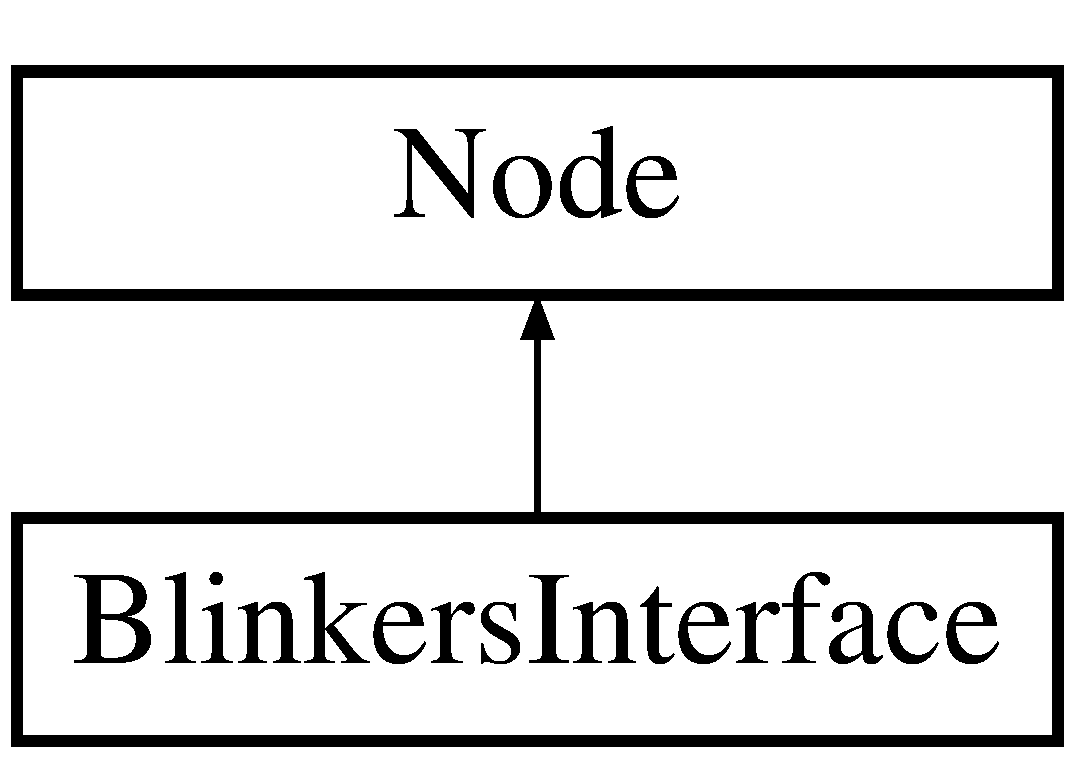
\includegraphics[height=2.000000cm]{db/db2/classtoxic__hardware_1_1blinkers__interface_1_1BlinkersInterface}
\end{center}
\end{figure}
\doxysubsection*{Public Member Functions}
\begin{DoxyCompactItemize}
\item 
def \mbox{\hyperlink{classtoxic__hardware_1_1blinkers__interface_1_1BlinkersInterface_ae64f0875afe3067b97ba370b354b9213}{\+\_\+\+\_\+init\+\_\+\+\_\+}} (self)
\item 
def \mbox{\hyperlink{classtoxic__hardware_1_1blinkers__interface_1_1BlinkersInterface_a74f43bc48b49ce4860b4fe27ab96fdda}{blinkers\+\_\+callback}} (self, data)
\item 
def \mbox{\hyperlink{classtoxic__hardware_1_1blinkers__interface_1_1BlinkersInterface_ae64f0875afe3067b97ba370b354b9213}{\+\_\+\+\_\+init\+\_\+\+\_\+}} (self)
\item 
def \mbox{\hyperlink{classtoxic__hardware_1_1blinkers__interface_1_1BlinkersInterface_a74f43bc48b49ce4860b4fe27ab96fdda}{blinkers\+\_\+callback}} (self, data)
\end{DoxyCompactItemize}
\doxysubsection*{Public Attributes}
\begin{DoxyCompactItemize}
\item 
\mbox{\hyperlink{classtoxic__hardware_1_1blinkers__interface_1_1BlinkersInterface_a4b0698733c4dfaffe8e2b4cd952b6f82}{subscription}}
\end{DoxyCompactItemize}


\doxysubsection{Constructor \& Destructor Documentation}
\mbox{\Hypertarget{classtoxic__hardware_1_1blinkers__interface_1_1BlinkersInterface_ae64f0875afe3067b97ba370b354b9213}\label{classtoxic__hardware_1_1blinkers__interface_1_1BlinkersInterface_ae64f0875afe3067b97ba370b354b9213}} 
\index{BlinkersInterface@{BlinkersInterface}!\_\_init\_\_@{\_\_init\_\_}}
\index{\_\_init\_\_@{\_\_init\_\_}!BlinkersInterface@{BlinkersInterface}}
\doxysubsubsection{\texorpdfstring{\_\_init\_\_()}{\_\_init\_\_()}\hspace{0.1cm}{\footnotesize\ttfamily [1/2]}}
{\footnotesize\ttfamily def \+\_\+\+\_\+init\+\_\+\+\_\+ (\begin{DoxyParamCaption}\item[{}]{self }\end{DoxyParamCaption})}


\begin{DoxyCode}{0}
\DoxyCodeLine{11     \textcolor{keyword}{def }\_\_init\_\_(self):}
\DoxyCodeLine{12         super().\_\_init\_\_(\textcolor{stringliteral}{'blinkers\_interface'})}
\DoxyCodeLine{13         self.subscription = self.create\_subscription(}
\DoxyCodeLine{14                 Int8,}
\DoxyCodeLine{15                 \textcolor{stringliteral}{'/blinkers'},}
\DoxyCodeLine{16                 self.blinkers\_callback,}
\DoxyCodeLine{17                 2}
\DoxyCodeLine{18                 )}
\DoxyCodeLine{19         self.subscription}
\DoxyCodeLine{20 }

\end{DoxyCode}
\mbox{\Hypertarget{classtoxic__hardware_1_1blinkers__interface_1_1BlinkersInterface_ae64f0875afe3067b97ba370b354b9213}\label{classtoxic__hardware_1_1blinkers__interface_1_1BlinkersInterface_ae64f0875afe3067b97ba370b354b9213}} 
\index{BlinkersInterface@{BlinkersInterface}!\_\_init\_\_@{\_\_init\_\_}}
\index{\_\_init\_\_@{\_\_init\_\_}!BlinkersInterface@{BlinkersInterface}}
\doxysubsubsection{\texorpdfstring{\_\_init\_\_()}{\_\_init\_\_()}\hspace{0.1cm}{\footnotesize\ttfamily [2/2]}}
{\footnotesize\ttfamily def \+\_\+\+\_\+init\+\_\+\+\_\+ (\begin{DoxyParamCaption}\item[{}]{self }\end{DoxyParamCaption})}


\begin{DoxyCode}{0}
\DoxyCodeLine{11     \textcolor{keyword}{def }\_\_init\_\_(self):}
\DoxyCodeLine{12         super().\_\_init\_\_(\textcolor{stringliteral}{'blinkers\_interface'})}
\DoxyCodeLine{13         self.subscription = self.create\_subscription(}
\DoxyCodeLine{14                 Int8,}
\DoxyCodeLine{15                 \textcolor{stringliteral}{'/blinkers'},}
\DoxyCodeLine{16                 self.blinkers\_callback,}
\DoxyCodeLine{17                 2}
\DoxyCodeLine{18                 )}
\DoxyCodeLine{19         self.subscription}
\DoxyCodeLine{20 }

\end{DoxyCode}


\doxysubsection{Member Function Documentation}
\mbox{\Hypertarget{classtoxic__hardware_1_1blinkers__interface_1_1BlinkersInterface_a74f43bc48b49ce4860b4fe27ab96fdda}\label{classtoxic__hardware_1_1blinkers__interface_1_1BlinkersInterface_a74f43bc48b49ce4860b4fe27ab96fdda}} 
\index{BlinkersInterface@{BlinkersInterface}!blinkers\_callback@{blinkers\_callback}}
\index{blinkers\_callback@{blinkers\_callback}!BlinkersInterface@{BlinkersInterface}}
\doxysubsubsection{\texorpdfstring{blinkers\_callback()}{blinkers\_callback()}\hspace{0.1cm}{\footnotesize\ttfamily [1/2]}}
{\footnotesize\ttfamily def blinkers\+\_\+callback (\begin{DoxyParamCaption}\item[{}]{self,  }\item[{}]{data }\end{DoxyParamCaption})}


\begin{DoxyCode}{0}
\DoxyCodeLine{21     \textcolor{keyword}{def }blinkers\_callback(self, data):}
\DoxyCodeLine{22         \textcolor{keyword}{global} gpio\_pin}
\DoxyCodeLine{23         recived = data.data}
\DoxyCodeLine{24         \textcolor{keywordflow}{if} recived == 0:}
\DoxyCodeLine{25             lgpio.gpio\_write(gpio\_pin, 17, 0)}
\DoxyCodeLine{26             lgpio.gpio\_write(gpio\_pin, 27, 0)}
\DoxyCodeLine{27         \textcolor{keywordflow}{elif} recived == 1:}
\DoxyCodeLine{28             lgpio.gpio\_write(gpio\_pin, 17, 1)}
\DoxyCodeLine{29             time.sleep(0.5)}
\DoxyCodeLine{30             lgpio.gpio\_write(gpio\_pin, 17, 0)}
\DoxyCodeLine{31             time.sleep(0.5)}
\DoxyCodeLine{32         \textcolor{keywordflow}{elif} recived == -\/1:}
\DoxyCodeLine{33             lgpio.gpio\_write(gpio\_pin, 27, 1)}
\DoxyCodeLine{34             time.sleep(0.5)}
\DoxyCodeLine{35             lgpio.gpio\_write(gpio\_pin, 27, 0)}
\DoxyCodeLine{36             time.sleep(0.5)}
\DoxyCodeLine{37         \textcolor{keywordflow}{else}:}
\DoxyCodeLine{38             lgpio.gpio\_write(gpio\_pin, 17, 1)}
\DoxyCodeLine{39             lgpio.gpio\_write(gpio\_pin, 27, 1)}
\DoxyCodeLine{40             time.sleep(0.5)}
\DoxyCodeLine{41             lgpio.gpio\_write(gpio\_pin, 17, 0)}
\DoxyCodeLine{42             lgpio.gpio\_write(gpio\_pin, 27, 0)}
\DoxyCodeLine{43             time.sleep(0.5)}
\DoxyCodeLine{44 }
\DoxyCodeLine{45 }

\end{DoxyCode}
\mbox{\Hypertarget{classtoxic__hardware_1_1blinkers__interface_1_1BlinkersInterface_a74f43bc48b49ce4860b4fe27ab96fdda}\label{classtoxic__hardware_1_1blinkers__interface_1_1BlinkersInterface_a74f43bc48b49ce4860b4fe27ab96fdda}} 
\index{BlinkersInterface@{BlinkersInterface}!blinkers\_callback@{blinkers\_callback}}
\index{blinkers\_callback@{blinkers\_callback}!BlinkersInterface@{BlinkersInterface}}
\doxysubsubsection{\texorpdfstring{blinkers\_callback()}{blinkers\_callback()}\hspace{0.1cm}{\footnotesize\ttfamily [2/2]}}
{\footnotesize\ttfamily def blinkers\+\_\+callback (\begin{DoxyParamCaption}\item[{}]{self,  }\item[{}]{data }\end{DoxyParamCaption})}


\begin{DoxyCode}{0}
\DoxyCodeLine{21     \textcolor{keyword}{def }blinkers\_callback(self, data):}
\DoxyCodeLine{22         \textcolor{keyword}{global} gpio\_pin}
\DoxyCodeLine{23         recived = data.data}
\DoxyCodeLine{24         \textcolor{keywordflow}{if} recived == 0:}
\DoxyCodeLine{25             lgpio.gpio\_write(gpio\_pin, 17, 0)}
\DoxyCodeLine{26             lgpio.gpio\_write(gpio\_pin, 27, 0)}
\DoxyCodeLine{27         \textcolor{keywordflow}{elif} recived == 1:}
\DoxyCodeLine{28             lgpio.gpio\_write(gpio\_pin, 17, 1)}
\DoxyCodeLine{29             time.sleep(0.5)}
\DoxyCodeLine{30             lgpio.gpio\_write(gpio\_pin, 17, 0)}
\DoxyCodeLine{31             time.sleep(0.5)}
\DoxyCodeLine{32         \textcolor{keywordflow}{elif} recived == -\/1:}
\DoxyCodeLine{33             lgpio.gpio\_write(gpio\_pin, 27, 1)}
\DoxyCodeLine{34             time.sleep(0.5)}
\DoxyCodeLine{35             lgpio.gpio\_write(gpio\_pin, 27, 0)}
\DoxyCodeLine{36             time.sleep(0.5)}
\DoxyCodeLine{37         \textcolor{keywordflow}{else}:}
\DoxyCodeLine{38             lgpio.gpio\_write(gpio\_pin, 17, 1)}
\DoxyCodeLine{39             lgpio.gpio\_write(gpio\_pin, 27, 1)}
\DoxyCodeLine{40             time.sleep(0.5)}
\DoxyCodeLine{41             lgpio.gpio\_write(gpio\_pin, 17, 0)}
\DoxyCodeLine{42             lgpio.gpio\_write(gpio\_pin, 27, 0)}
\DoxyCodeLine{43             time.sleep(0.5)}
\DoxyCodeLine{44 }
\DoxyCodeLine{45 }

\end{DoxyCode}


\doxysubsection{Member Data Documentation}
\mbox{\Hypertarget{classtoxic__hardware_1_1blinkers__interface_1_1BlinkersInterface_a4b0698733c4dfaffe8e2b4cd952b6f82}\label{classtoxic__hardware_1_1blinkers__interface_1_1BlinkersInterface_a4b0698733c4dfaffe8e2b4cd952b6f82}} 
\index{BlinkersInterface@{BlinkersInterface}!subscription@{subscription}}
\index{subscription@{subscription}!BlinkersInterface@{BlinkersInterface}}
\doxysubsubsection{\texorpdfstring{subscription}{subscription}}
{\footnotesize\ttfamily subscription}



The documentation for this class was generated from the following file\+:\begin{DoxyCompactItemize}
\item 
main\+\_\+ws/build/toxic\+\_\+hardware/build/lib/toxic\+\_\+hardware/\mbox{\hyperlink{build_2toxic__hardware_2build_2lib_2toxic__hardware_2blinkers__interface_8py}{blinkers\+\_\+interface.\+py}}\end{DoxyCompactItemize}

\hypertarget{classtoxic__hardware_1_1roboclaw__3_1_1Roboclaw_1_1Cmd}{}\doxysection{Roboclaw.\+Cmd Class Reference}
\label{classtoxic__hardware_1_1roboclaw__3_1_1Roboclaw_1_1Cmd}\index{Roboclaw.Cmd@{Roboclaw.Cmd}}
\doxysubsection*{Static Public Attributes}
\begin{DoxyCompactItemize}
\item 
int \mbox{\hyperlink{classtoxic__hardware_1_1roboclaw__3_1_1Roboclaw_1_1Cmd_a6fbd0a7399dbe49e1c4f10320a0bce05}{M1\+FORWARD}} = 0
\item 
int \mbox{\hyperlink{classtoxic__hardware_1_1roboclaw__3_1_1Roboclaw_1_1Cmd_aaddaee1e3f47d2dea0606ba42f9ae366}{M1\+BACKWARD}} = 1
\item 
int \mbox{\hyperlink{classtoxic__hardware_1_1roboclaw__3_1_1Roboclaw_1_1Cmd_aec7863ce95adb6df8cdd805f03308333}{SETMINMB}} = 2
\item 
int \mbox{\hyperlink{classtoxic__hardware_1_1roboclaw__3_1_1Roboclaw_1_1Cmd_ae9073696e45e2bd9fc89ea7ac55c9241}{SETMAXMB}} = 3
\item 
int \mbox{\hyperlink{classtoxic__hardware_1_1roboclaw__3_1_1Roboclaw_1_1Cmd_a2b83b23d87ba642f2f3bc98a1c761851}{M2\+FORWARD}} = 4
\item 
int \mbox{\hyperlink{classtoxic__hardware_1_1roboclaw__3_1_1Roboclaw_1_1Cmd_a74857241586e205cacf8b88815b12e40}{M2\+BACKWARD}} = 5
\item 
int \mbox{\hyperlink{classtoxic__hardware_1_1roboclaw__3_1_1Roboclaw_1_1Cmd_a40c2006f4b2590d5afb118137d899e2b}{M17\+BIT}} = 6
\item 
int \mbox{\hyperlink{classtoxic__hardware_1_1roboclaw__3_1_1Roboclaw_1_1Cmd_ad760450d0f321d75a1194c5eb6af154c}{M27\+BIT}} = 7
\item 
int \mbox{\hyperlink{classtoxic__hardware_1_1roboclaw__3_1_1Roboclaw_1_1Cmd_a1fdd8dee03e0e259170950830ff13cf5}{MIXEDFORWARD}} = 8
\item 
int \mbox{\hyperlink{classtoxic__hardware_1_1roboclaw__3_1_1Roboclaw_1_1Cmd_a33530a0c1fd0ea54e33982788e9e5663}{MIXEDBACKWARD}} = 9
\item 
int \mbox{\hyperlink{classtoxic__hardware_1_1roboclaw__3_1_1Roboclaw_1_1Cmd_a398bed0c793dc5fb515257786803fa29}{MIXEDRIGHT}} = 10
\item 
int \mbox{\hyperlink{classtoxic__hardware_1_1roboclaw__3_1_1Roboclaw_1_1Cmd_a490c0e33c039db2a101cd923f790846a}{MIXEDLEFT}} = 11
\item 
int \mbox{\hyperlink{classtoxic__hardware_1_1roboclaw__3_1_1Roboclaw_1_1Cmd_a99317b16d68833586aceaeab96f25bb9}{MIXEDFB}} = 12
\item 
int \mbox{\hyperlink{classtoxic__hardware_1_1roboclaw__3_1_1Roboclaw_1_1Cmd_abae324df58695821b0ae79d651237aa4}{MIXEDLR}} = 13
\item 
int \mbox{\hyperlink{classtoxic__hardware_1_1roboclaw__3_1_1Roboclaw_1_1Cmd_ac0ba87709e343a9a635b2035e193b8c4}{GETM1\+ENC}} = 16
\item 
int \mbox{\hyperlink{classtoxic__hardware_1_1roboclaw__3_1_1Roboclaw_1_1Cmd_a209d097653ba57f987ad09c1931a855a}{GETM2\+ENC}} = 17
\item 
int \mbox{\hyperlink{classtoxic__hardware_1_1roboclaw__3_1_1Roboclaw_1_1Cmd_af38550f1924f8645a650d2944505f660}{GETM1\+SPEED}} = 18
\item 
int \mbox{\hyperlink{classtoxic__hardware_1_1roboclaw__3_1_1Roboclaw_1_1Cmd_afc30cd26545456254e617e0bbc337c72}{GETM2\+SPEED}} = 19
\item 
int \mbox{\hyperlink{classtoxic__hardware_1_1roboclaw__3_1_1Roboclaw_1_1Cmd_ad8c64e5070504bfe803b7966aa0775e0}{RESETENC}} = 20
\item 
int \mbox{\hyperlink{classtoxic__hardware_1_1roboclaw__3_1_1Roboclaw_1_1Cmd_a73f2fa42c1a05d7aae2776b174e21703}{GETVERSION}} = 21
\item 
int \mbox{\hyperlink{classtoxic__hardware_1_1roboclaw__3_1_1Roboclaw_1_1Cmd_ac8fb2a2de19659e407763c3ecdb2afeb}{SETM1\+ENCCOUNT}} = 22
\item 
int \mbox{\hyperlink{classtoxic__hardware_1_1roboclaw__3_1_1Roboclaw_1_1Cmd_a60085be8abee824c10374c00b7e960d4}{SETM2\+ENCCOUNT}} = 23
\item 
int \mbox{\hyperlink{classtoxic__hardware_1_1roboclaw__3_1_1Roboclaw_1_1Cmd_ae74486177b4bd6990de30aec301f3116}{GETMBATT}} = 24
\item 
int \mbox{\hyperlink{classtoxic__hardware_1_1roboclaw__3_1_1Roboclaw_1_1Cmd_a7e209901456188c2fb77c112b69a72d7}{GETLBATT}} = 25
\item 
int \mbox{\hyperlink{classtoxic__hardware_1_1roboclaw__3_1_1Roboclaw_1_1Cmd_aca2add1deb9b7fd9010c5e6e6b0c5a82}{SETMINLB}} = 26
\item 
int \mbox{\hyperlink{classtoxic__hardware_1_1roboclaw__3_1_1Roboclaw_1_1Cmd_a7df411501d297e2450b2985adb90e500}{SETMAXLB}} = 27
\item 
int \mbox{\hyperlink{classtoxic__hardware_1_1roboclaw__3_1_1Roboclaw_1_1Cmd_a4dd28dabd2f5c8e7cd3637601fdf7ebb}{SETM1\+PID}} = 28
\item 
int \mbox{\hyperlink{classtoxic__hardware_1_1roboclaw__3_1_1Roboclaw_1_1Cmd_ab8729410adde6d43c8dfb809e27e5791}{SETM2\+PID}} = 29
\item 
int \mbox{\hyperlink{classtoxic__hardware_1_1roboclaw__3_1_1Roboclaw_1_1Cmd_a3ab756a8cf452c40ba9660aa7db3d56c}{GETM1\+ISPEED}} = 30
\item 
int \mbox{\hyperlink{classtoxic__hardware_1_1roboclaw__3_1_1Roboclaw_1_1Cmd_a130a8997fe5069570b363cea0a0e08c6}{GETM2\+ISPEED}} = 31
\item 
int \mbox{\hyperlink{classtoxic__hardware_1_1roboclaw__3_1_1Roboclaw_1_1Cmd_a984c7f0e95d28f85ad5f4bcfd1f6d948}{M1\+DUTY}} = 32
\item 
int \mbox{\hyperlink{classtoxic__hardware_1_1roboclaw__3_1_1Roboclaw_1_1Cmd_afd0f106fa9ae418773b03a47ca7d3774}{M2\+DUTY}} = 33
\item 
int \mbox{\hyperlink{classtoxic__hardware_1_1roboclaw__3_1_1Roboclaw_1_1Cmd_afcb0f018c30e447aee21b998b73f2849}{MIXEDDUTY}} = 34
\item 
int \mbox{\hyperlink{classtoxic__hardware_1_1roboclaw__3_1_1Roboclaw_1_1Cmd_a162588561112dc25f1f61d76adccfe3a}{M1\+SPEED}} = 35
\item 
int \mbox{\hyperlink{classtoxic__hardware_1_1roboclaw__3_1_1Roboclaw_1_1Cmd_af310518147f926879260a6cc117155f9}{M2\+SPEED}} = 36
\item 
int \mbox{\hyperlink{classtoxic__hardware_1_1roboclaw__3_1_1Roboclaw_1_1Cmd_aad8674b20c62b1a1f7bafdb9c2a59db2}{MIXEDSPEED}} = 37
\item 
int \mbox{\hyperlink{classtoxic__hardware_1_1roboclaw__3_1_1Roboclaw_1_1Cmd_a9266a50e5460b6f117bf3ed523aa3639}{M1\+SPEEDACCEL}} = 38
\item 
int \mbox{\hyperlink{classtoxic__hardware_1_1roboclaw__3_1_1Roboclaw_1_1Cmd_abf84b765d58fe103fd3c051ac629ed0e}{M2\+SPEEDACCEL}} = 39
\item 
int \mbox{\hyperlink{classtoxic__hardware_1_1roboclaw__3_1_1Roboclaw_1_1Cmd_a306a7796d0376174333e7d3f63911941}{MIXEDSPEEDACCEL}} = 40
\item 
int \mbox{\hyperlink{classtoxic__hardware_1_1roboclaw__3_1_1Roboclaw_1_1Cmd_a02ad57ac2088ecadb26323dd94349cc4}{M1\+SPEEDDIST}} = 41
\item 
int \mbox{\hyperlink{classtoxic__hardware_1_1roboclaw__3_1_1Roboclaw_1_1Cmd_add22920c1ebb1d0e13f0017474d212dc}{M2\+SPEEDDIST}} = 42
\item 
int \mbox{\hyperlink{classtoxic__hardware_1_1roboclaw__3_1_1Roboclaw_1_1Cmd_a17c41e60e8e0ef3b1d46465936e3c9bf}{MIXEDSPEEDDIST}} = 43
\item 
int \mbox{\hyperlink{classtoxic__hardware_1_1roboclaw__3_1_1Roboclaw_1_1Cmd_ae0cc23d22e15a200b9bc782346a54738}{M1\+SPEEDACCELDIST}} = 44
\item 
int \mbox{\hyperlink{classtoxic__hardware_1_1roboclaw__3_1_1Roboclaw_1_1Cmd_a47ee184dd1cfd86291f58aced7de3821}{M2\+SPEEDACCELDIST}} = 45
\item 
int \mbox{\hyperlink{classtoxic__hardware_1_1roboclaw__3_1_1Roboclaw_1_1Cmd_a7823fd7565a2e72f7a972b2fd517a985}{MIXEDSPEEDACCELDIST}} = 46
\item 
int \mbox{\hyperlink{classtoxic__hardware_1_1roboclaw__3_1_1Roboclaw_1_1Cmd_ad36eda4158a5215ae5ee52401d24e39b}{GETBUFFERS}} = 47
\item 
int \mbox{\hyperlink{classtoxic__hardware_1_1roboclaw__3_1_1Roboclaw_1_1Cmd_aba1e3d225a2a3c61d8a2f2ce2f062d9c}{GETPWMS}} = 48
\item 
int \mbox{\hyperlink{classtoxic__hardware_1_1roboclaw__3_1_1Roboclaw_1_1Cmd_a7b8aa436bab3175fc6904b1a9e790821}{GETCURRENTS}} = 49
\item 
int \mbox{\hyperlink{classtoxic__hardware_1_1roboclaw__3_1_1Roboclaw_1_1Cmd_a075704022e7f303e509ecd4da010050f}{MIXEDSPEED2\+ACCEL}} = 50
\item 
int \mbox{\hyperlink{classtoxic__hardware_1_1roboclaw__3_1_1Roboclaw_1_1Cmd_ae6218e53fcba38d3e0f217b83fa74275}{MIXEDSPEED2\+ACCELDIST}} = 51
\item 
int \mbox{\hyperlink{classtoxic__hardware_1_1roboclaw__3_1_1Roboclaw_1_1Cmd_a0c3dd728d7b7946fb5e3d5febe55e15a}{M1\+DUTYACCEL}} = 52
\item 
int \mbox{\hyperlink{classtoxic__hardware_1_1roboclaw__3_1_1Roboclaw_1_1Cmd_ae4fd74abec7fef3501358139af2afdb2}{M2\+DUTYACCEL}} = 53
\item 
int \mbox{\hyperlink{classtoxic__hardware_1_1roboclaw__3_1_1Roboclaw_1_1Cmd_a90760f994a82bf29c7dce267809fc53f}{MIXEDDUTYACCEL}} = 54
\item 
int \mbox{\hyperlink{classtoxic__hardware_1_1roboclaw__3_1_1Roboclaw_1_1Cmd_a4b160e11dcc7fce108996fc7b73988bf}{READM1\+PID}} = 55
\item 
int \mbox{\hyperlink{classtoxic__hardware_1_1roboclaw__3_1_1Roboclaw_1_1Cmd_afcb1ce02ede2d4a11ef044017b7df62b}{READM2\+PID}} = 56
\item 
int \mbox{\hyperlink{classtoxic__hardware_1_1roboclaw__3_1_1Roboclaw_1_1Cmd_a2ae5605f820e3846ea5854bf74dd9a02}{SETMAINVOLTAGES}} = 57
\item 
int \mbox{\hyperlink{classtoxic__hardware_1_1roboclaw__3_1_1Roboclaw_1_1Cmd_a12fa895e88adfe911799fefbe6a24ea5}{SETLOGICVOLTAGES}} = 58
\item 
int \mbox{\hyperlink{classtoxic__hardware_1_1roboclaw__3_1_1Roboclaw_1_1Cmd_a371c46088a7d76f11306c9e74ffc9976}{GETMINMAXMAINVOLTAGES}} = 59
\item 
int \mbox{\hyperlink{classtoxic__hardware_1_1roboclaw__3_1_1Roboclaw_1_1Cmd_a16f67765c09e5c136fff72d30b50cced}{GETMINMAXLOGICVOLTAGES}} = 60
\item 
int \mbox{\hyperlink{classtoxic__hardware_1_1roboclaw__3_1_1Roboclaw_1_1Cmd_a51f15162c2c690d760415ddb20a12680}{SETM1\+POSPID}} = 61
\item 
int \mbox{\hyperlink{classtoxic__hardware_1_1roboclaw__3_1_1Roboclaw_1_1Cmd_adc37ab96c5ba37c298cb5f8d2df7cd06}{SETM2\+POSPID}} = 62
\item 
int \mbox{\hyperlink{classtoxic__hardware_1_1roboclaw__3_1_1Roboclaw_1_1Cmd_a6f0db6750f2f2e720deec2086ef29ed0}{READM1\+POSPID}} = 63
\item 
int \mbox{\hyperlink{classtoxic__hardware_1_1roboclaw__3_1_1Roboclaw_1_1Cmd_a3a94ad96d31a215bc7edf68001ed3be2}{READM2\+POSPID}} = 64
\item 
int \mbox{\hyperlink{classtoxic__hardware_1_1roboclaw__3_1_1Roboclaw_1_1Cmd_a10674481f4a98e4d62d390e80f4072d6}{M1\+SPEEDACCELDECCELPOS}} = 65
\item 
int \mbox{\hyperlink{classtoxic__hardware_1_1roboclaw__3_1_1Roboclaw_1_1Cmd_ad5c8ed695c618fcd1a34eff386e69168}{M2\+SPEEDACCELDECCELPOS}} = 66
\item 
int \mbox{\hyperlink{classtoxic__hardware_1_1roboclaw__3_1_1Roboclaw_1_1Cmd_a30cc75003a8d5bc716aef28f316174f4}{MIXEDSPEEDACCELDECCELPOS}} = 67
\item 
int \mbox{\hyperlink{classtoxic__hardware_1_1roboclaw__3_1_1Roboclaw_1_1Cmd_a58a545204a0df366fdc87d0f5be41fc0}{SETM1\+DEFAULTACCEL}} = 68
\item 
int \mbox{\hyperlink{classtoxic__hardware_1_1roboclaw__3_1_1Roboclaw_1_1Cmd_a4641384c4279e5469e1658c768956038}{SETM2\+DEFAULTACCEL}} = 69
\item 
int \mbox{\hyperlink{classtoxic__hardware_1_1roboclaw__3_1_1Roboclaw_1_1Cmd_a0038406619934114793ed744b352a256}{SETPINFUNCTIONS}} = 74
\item 
int \mbox{\hyperlink{classtoxic__hardware_1_1roboclaw__3_1_1Roboclaw_1_1Cmd_a2d797bf95e4febe4b3b6b5ace42400cb}{GETPINFUNCTIONS}} = 75
\item 
int \mbox{\hyperlink{classtoxic__hardware_1_1roboclaw__3_1_1Roboclaw_1_1Cmd_a473dc616d63cd06a3e09c73ce1622f81}{SETDEADBAND}} = 76
\item 
int \mbox{\hyperlink{classtoxic__hardware_1_1roboclaw__3_1_1Roboclaw_1_1Cmd_aeecde73b79be340729647ba9e5fcb747}{GETDEADBAND}} = 77
\item 
int \mbox{\hyperlink{classtoxic__hardware_1_1roboclaw__3_1_1Roboclaw_1_1Cmd_ae3df67bf8e3c9bf14b5c6aef9d06430e}{RESTOREDEFAULTS}} = 80
\item 
int \mbox{\hyperlink{classtoxic__hardware_1_1roboclaw__3_1_1Roboclaw_1_1Cmd_a73c91975f9b88c9f094b0fb0f9947f4a}{GETTEMP}} = 82
\item 
int \mbox{\hyperlink{classtoxic__hardware_1_1roboclaw__3_1_1Roboclaw_1_1Cmd_a17e151c522e0d133d2640a66bf483c7d}{GETTEMP2}} = 83
\item 
int \mbox{\hyperlink{classtoxic__hardware_1_1roboclaw__3_1_1Roboclaw_1_1Cmd_a902a86118ed630c45aead64b567be4e5}{GETERROR}} = 90
\item 
int \mbox{\hyperlink{classtoxic__hardware_1_1roboclaw__3_1_1Roboclaw_1_1Cmd_a4e654ec397b1745472d5e87df78b9a79}{GETENCODERMODE}} = 91
\item 
int \mbox{\hyperlink{classtoxic__hardware_1_1roboclaw__3_1_1Roboclaw_1_1Cmd_a0ebbf9388c096edda037ef2940ff8939}{SETM1\+ENCODERMODE}} = 92
\item 
int \mbox{\hyperlink{classtoxic__hardware_1_1roboclaw__3_1_1Roboclaw_1_1Cmd_ab8ccfdee1f527090a2e1bedcfc6bb65d}{SETM2\+ENCODERMODE}} = 93
\item 
int \mbox{\hyperlink{classtoxic__hardware_1_1roboclaw__3_1_1Roboclaw_1_1Cmd_ab7ad074d286dccbe386cbf9ff2157fdd}{WRITENVM}} = 94
\item 
int \mbox{\hyperlink{classtoxic__hardware_1_1roboclaw__3_1_1Roboclaw_1_1Cmd_ad70382e38639bfa11c90f3b92e3b9dfe}{READNVM}} = 95
\item 
int \mbox{\hyperlink{classtoxic__hardware_1_1roboclaw__3_1_1Roboclaw_1_1Cmd_a8ee1b998b269bcc6cf0d84895a2f2d9f}{SETCONFIG}} = 98
\item 
int \mbox{\hyperlink{classtoxic__hardware_1_1roboclaw__3_1_1Roboclaw_1_1Cmd_a779f8c61d9941e3c201f0aba886a17f2}{GETCONFIG}} = 99
\item 
int \mbox{\hyperlink{classtoxic__hardware_1_1roboclaw__3_1_1Roboclaw_1_1Cmd_ac9eda5476e71091de99ace27c88df633}{SETM1\+MAXCURRENT}} = 133
\item 
int \mbox{\hyperlink{classtoxic__hardware_1_1roboclaw__3_1_1Roboclaw_1_1Cmd_a380ae8336824145de8f46340f5160290}{SETM2\+MAXCURRENT}} = 134
\item 
int \mbox{\hyperlink{classtoxic__hardware_1_1roboclaw__3_1_1Roboclaw_1_1Cmd_a4f34b6a343d8e39b46fdf6dc046d336c}{GETM1\+MAXCURRENT}} = 135
\item 
int \mbox{\hyperlink{classtoxic__hardware_1_1roboclaw__3_1_1Roboclaw_1_1Cmd_ae809a9cb7e9925a7bec93f1d50aa26f0}{GETM2\+MAXCURRENT}} = 136
\item 
int \mbox{\hyperlink{classtoxic__hardware_1_1roboclaw__3_1_1Roboclaw_1_1Cmd_ada01acd049241528247c85758a1f18f1}{SETPWMMODE}} = 148
\item 
int \mbox{\hyperlink{classtoxic__hardware_1_1roboclaw__3_1_1Roboclaw_1_1Cmd_a4623c878bfa3801984ed9b029ec26839}{GETPWMMODE}} = 149
\item 
int \mbox{\hyperlink{classtoxic__hardware_1_1roboclaw__3_1_1Roboclaw_1_1Cmd_a92a69eadf0f81f653a6f74be93a150f0}{READEEPROM}} = 252
\item 
int \mbox{\hyperlink{classtoxic__hardware_1_1roboclaw__3_1_1Roboclaw_1_1Cmd_a3f5df487bb061c8072c3e39eef15abd4}{WRITEEEPROM}} = 253
\item 
int \mbox{\hyperlink{classtoxic__hardware_1_1roboclaw__3_1_1Roboclaw_1_1Cmd_ac3d1533d23fc8092582fc55bcd116ede}{FLAGBOOTLOADER}} = 255
\end{DoxyCompactItemize}


\doxysubsection{Member Data Documentation}
\mbox{\Hypertarget{classtoxic__hardware_1_1roboclaw__3_1_1Roboclaw_1_1Cmd_ac3d1533d23fc8092582fc55bcd116ede}\label{classtoxic__hardware_1_1roboclaw__3_1_1Roboclaw_1_1Cmd_ac3d1533d23fc8092582fc55bcd116ede}} 
\index{Roboclaw.Cmd@{Roboclaw.Cmd}!FLAGBOOTLOADER@{FLAGBOOTLOADER}}
\index{FLAGBOOTLOADER@{FLAGBOOTLOADER}!Roboclaw.Cmd@{Roboclaw.Cmd}}
\doxysubsubsection{\texorpdfstring{FLAGBOOTLOADER}{FLAGBOOTLOADER}}
{\footnotesize\ttfamily int FLAGBOOTLOADER = 255\hspace{0.3cm}{\ttfamily [static]}}

\mbox{\Hypertarget{classtoxic__hardware_1_1roboclaw__3_1_1Roboclaw_1_1Cmd_ad36eda4158a5215ae5ee52401d24e39b}\label{classtoxic__hardware_1_1roboclaw__3_1_1Roboclaw_1_1Cmd_ad36eda4158a5215ae5ee52401d24e39b}} 
\index{Roboclaw.Cmd@{Roboclaw.Cmd}!GETBUFFERS@{GETBUFFERS}}
\index{GETBUFFERS@{GETBUFFERS}!Roboclaw.Cmd@{Roboclaw.Cmd}}
\doxysubsubsection{\texorpdfstring{GETBUFFERS}{GETBUFFERS}}
{\footnotesize\ttfamily int GETBUFFERS = 47\hspace{0.3cm}{\ttfamily [static]}}

\mbox{\Hypertarget{classtoxic__hardware_1_1roboclaw__3_1_1Roboclaw_1_1Cmd_a779f8c61d9941e3c201f0aba886a17f2}\label{classtoxic__hardware_1_1roboclaw__3_1_1Roboclaw_1_1Cmd_a779f8c61d9941e3c201f0aba886a17f2}} 
\index{Roboclaw.Cmd@{Roboclaw.Cmd}!GETCONFIG@{GETCONFIG}}
\index{GETCONFIG@{GETCONFIG}!Roboclaw.Cmd@{Roboclaw.Cmd}}
\doxysubsubsection{\texorpdfstring{GETCONFIG}{GETCONFIG}}
{\footnotesize\ttfamily int GETCONFIG = 99\hspace{0.3cm}{\ttfamily [static]}}

\mbox{\Hypertarget{classtoxic__hardware_1_1roboclaw__3_1_1Roboclaw_1_1Cmd_a7b8aa436bab3175fc6904b1a9e790821}\label{classtoxic__hardware_1_1roboclaw__3_1_1Roboclaw_1_1Cmd_a7b8aa436bab3175fc6904b1a9e790821}} 
\index{Roboclaw.Cmd@{Roboclaw.Cmd}!GETCURRENTS@{GETCURRENTS}}
\index{GETCURRENTS@{GETCURRENTS}!Roboclaw.Cmd@{Roboclaw.Cmd}}
\doxysubsubsection{\texorpdfstring{GETCURRENTS}{GETCURRENTS}}
{\footnotesize\ttfamily int GETCURRENTS = 49\hspace{0.3cm}{\ttfamily [static]}}

\mbox{\Hypertarget{classtoxic__hardware_1_1roboclaw__3_1_1Roboclaw_1_1Cmd_aeecde73b79be340729647ba9e5fcb747}\label{classtoxic__hardware_1_1roboclaw__3_1_1Roboclaw_1_1Cmd_aeecde73b79be340729647ba9e5fcb747}} 
\index{Roboclaw.Cmd@{Roboclaw.Cmd}!GETDEADBAND@{GETDEADBAND}}
\index{GETDEADBAND@{GETDEADBAND}!Roboclaw.Cmd@{Roboclaw.Cmd}}
\doxysubsubsection{\texorpdfstring{GETDEADBAND}{GETDEADBAND}}
{\footnotesize\ttfamily int GETDEADBAND = 77\hspace{0.3cm}{\ttfamily [static]}}

\mbox{\Hypertarget{classtoxic__hardware_1_1roboclaw__3_1_1Roboclaw_1_1Cmd_a4e654ec397b1745472d5e87df78b9a79}\label{classtoxic__hardware_1_1roboclaw__3_1_1Roboclaw_1_1Cmd_a4e654ec397b1745472d5e87df78b9a79}} 
\index{Roboclaw.Cmd@{Roboclaw.Cmd}!GETENCODERMODE@{GETENCODERMODE}}
\index{GETENCODERMODE@{GETENCODERMODE}!Roboclaw.Cmd@{Roboclaw.Cmd}}
\doxysubsubsection{\texorpdfstring{GETENCODERMODE}{GETENCODERMODE}}
{\footnotesize\ttfamily int GETENCODERMODE = 91\hspace{0.3cm}{\ttfamily [static]}}

\mbox{\Hypertarget{classtoxic__hardware_1_1roboclaw__3_1_1Roboclaw_1_1Cmd_a902a86118ed630c45aead64b567be4e5}\label{classtoxic__hardware_1_1roboclaw__3_1_1Roboclaw_1_1Cmd_a902a86118ed630c45aead64b567be4e5}} 
\index{Roboclaw.Cmd@{Roboclaw.Cmd}!GETERROR@{GETERROR}}
\index{GETERROR@{GETERROR}!Roboclaw.Cmd@{Roboclaw.Cmd}}
\doxysubsubsection{\texorpdfstring{GETERROR}{GETERROR}}
{\footnotesize\ttfamily int GETERROR = 90\hspace{0.3cm}{\ttfamily [static]}}

\mbox{\Hypertarget{classtoxic__hardware_1_1roboclaw__3_1_1Roboclaw_1_1Cmd_a7e209901456188c2fb77c112b69a72d7}\label{classtoxic__hardware_1_1roboclaw__3_1_1Roboclaw_1_1Cmd_a7e209901456188c2fb77c112b69a72d7}} 
\index{Roboclaw.Cmd@{Roboclaw.Cmd}!GETLBATT@{GETLBATT}}
\index{GETLBATT@{GETLBATT}!Roboclaw.Cmd@{Roboclaw.Cmd}}
\doxysubsubsection{\texorpdfstring{GETLBATT}{GETLBATT}}
{\footnotesize\ttfamily int GETLBATT = 25\hspace{0.3cm}{\ttfamily [static]}}

\mbox{\Hypertarget{classtoxic__hardware_1_1roboclaw__3_1_1Roboclaw_1_1Cmd_ac0ba87709e343a9a635b2035e193b8c4}\label{classtoxic__hardware_1_1roboclaw__3_1_1Roboclaw_1_1Cmd_ac0ba87709e343a9a635b2035e193b8c4}} 
\index{Roboclaw.Cmd@{Roboclaw.Cmd}!GETM1ENC@{GETM1ENC}}
\index{GETM1ENC@{GETM1ENC}!Roboclaw.Cmd@{Roboclaw.Cmd}}
\doxysubsubsection{\texorpdfstring{GETM1ENC}{GETM1ENC}}
{\footnotesize\ttfamily int GETM1\+ENC = 16\hspace{0.3cm}{\ttfamily [static]}}

\mbox{\Hypertarget{classtoxic__hardware_1_1roboclaw__3_1_1Roboclaw_1_1Cmd_a3ab756a8cf452c40ba9660aa7db3d56c}\label{classtoxic__hardware_1_1roboclaw__3_1_1Roboclaw_1_1Cmd_a3ab756a8cf452c40ba9660aa7db3d56c}} 
\index{Roboclaw.Cmd@{Roboclaw.Cmd}!GETM1ISPEED@{GETM1ISPEED}}
\index{GETM1ISPEED@{GETM1ISPEED}!Roboclaw.Cmd@{Roboclaw.Cmd}}
\doxysubsubsection{\texorpdfstring{GETM1ISPEED}{GETM1ISPEED}}
{\footnotesize\ttfamily int GETM1\+ISPEED = 30\hspace{0.3cm}{\ttfamily [static]}}

\mbox{\Hypertarget{classtoxic__hardware_1_1roboclaw__3_1_1Roboclaw_1_1Cmd_a4f34b6a343d8e39b46fdf6dc046d336c}\label{classtoxic__hardware_1_1roboclaw__3_1_1Roboclaw_1_1Cmd_a4f34b6a343d8e39b46fdf6dc046d336c}} 
\index{Roboclaw.Cmd@{Roboclaw.Cmd}!GETM1MAXCURRENT@{GETM1MAXCURRENT}}
\index{GETM1MAXCURRENT@{GETM1MAXCURRENT}!Roboclaw.Cmd@{Roboclaw.Cmd}}
\doxysubsubsection{\texorpdfstring{GETM1MAXCURRENT}{GETM1MAXCURRENT}}
{\footnotesize\ttfamily int GETM1\+MAXCURRENT = 135\hspace{0.3cm}{\ttfamily [static]}}

\mbox{\Hypertarget{classtoxic__hardware_1_1roboclaw__3_1_1Roboclaw_1_1Cmd_af38550f1924f8645a650d2944505f660}\label{classtoxic__hardware_1_1roboclaw__3_1_1Roboclaw_1_1Cmd_af38550f1924f8645a650d2944505f660}} 
\index{Roboclaw.Cmd@{Roboclaw.Cmd}!GETM1SPEED@{GETM1SPEED}}
\index{GETM1SPEED@{GETM1SPEED}!Roboclaw.Cmd@{Roboclaw.Cmd}}
\doxysubsubsection{\texorpdfstring{GETM1SPEED}{GETM1SPEED}}
{\footnotesize\ttfamily int GETM1\+SPEED = 18\hspace{0.3cm}{\ttfamily [static]}}

\mbox{\Hypertarget{classtoxic__hardware_1_1roboclaw__3_1_1Roboclaw_1_1Cmd_a209d097653ba57f987ad09c1931a855a}\label{classtoxic__hardware_1_1roboclaw__3_1_1Roboclaw_1_1Cmd_a209d097653ba57f987ad09c1931a855a}} 
\index{Roboclaw.Cmd@{Roboclaw.Cmd}!GETM2ENC@{GETM2ENC}}
\index{GETM2ENC@{GETM2ENC}!Roboclaw.Cmd@{Roboclaw.Cmd}}
\doxysubsubsection{\texorpdfstring{GETM2ENC}{GETM2ENC}}
{\footnotesize\ttfamily int GETM2\+ENC = 17\hspace{0.3cm}{\ttfamily [static]}}

\mbox{\Hypertarget{classtoxic__hardware_1_1roboclaw__3_1_1Roboclaw_1_1Cmd_a130a8997fe5069570b363cea0a0e08c6}\label{classtoxic__hardware_1_1roboclaw__3_1_1Roboclaw_1_1Cmd_a130a8997fe5069570b363cea0a0e08c6}} 
\index{Roboclaw.Cmd@{Roboclaw.Cmd}!GETM2ISPEED@{GETM2ISPEED}}
\index{GETM2ISPEED@{GETM2ISPEED}!Roboclaw.Cmd@{Roboclaw.Cmd}}
\doxysubsubsection{\texorpdfstring{GETM2ISPEED}{GETM2ISPEED}}
{\footnotesize\ttfamily int GETM2\+ISPEED = 31\hspace{0.3cm}{\ttfamily [static]}}

\mbox{\Hypertarget{classtoxic__hardware_1_1roboclaw__3_1_1Roboclaw_1_1Cmd_ae809a9cb7e9925a7bec93f1d50aa26f0}\label{classtoxic__hardware_1_1roboclaw__3_1_1Roboclaw_1_1Cmd_ae809a9cb7e9925a7bec93f1d50aa26f0}} 
\index{Roboclaw.Cmd@{Roboclaw.Cmd}!GETM2MAXCURRENT@{GETM2MAXCURRENT}}
\index{GETM2MAXCURRENT@{GETM2MAXCURRENT}!Roboclaw.Cmd@{Roboclaw.Cmd}}
\doxysubsubsection{\texorpdfstring{GETM2MAXCURRENT}{GETM2MAXCURRENT}}
{\footnotesize\ttfamily int GETM2\+MAXCURRENT = 136\hspace{0.3cm}{\ttfamily [static]}}

\mbox{\Hypertarget{classtoxic__hardware_1_1roboclaw__3_1_1Roboclaw_1_1Cmd_afc30cd26545456254e617e0bbc337c72}\label{classtoxic__hardware_1_1roboclaw__3_1_1Roboclaw_1_1Cmd_afc30cd26545456254e617e0bbc337c72}} 
\index{Roboclaw.Cmd@{Roboclaw.Cmd}!GETM2SPEED@{GETM2SPEED}}
\index{GETM2SPEED@{GETM2SPEED}!Roboclaw.Cmd@{Roboclaw.Cmd}}
\doxysubsubsection{\texorpdfstring{GETM2SPEED}{GETM2SPEED}}
{\footnotesize\ttfamily int GETM2\+SPEED = 19\hspace{0.3cm}{\ttfamily [static]}}

\mbox{\Hypertarget{classtoxic__hardware_1_1roboclaw__3_1_1Roboclaw_1_1Cmd_ae74486177b4bd6990de30aec301f3116}\label{classtoxic__hardware_1_1roboclaw__3_1_1Roboclaw_1_1Cmd_ae74486177b4bd6990de30aec301f3116}} 
\index{Roboclaw.Cmd@{Roboclaw.Cmd}!GETMBATT@{GETMBATT}}
\index{GETMBATT@{GETMBATT}!Roboclaw.Cmd@{Roboclaw.Cmd}}
\doxysubsubsection{\texorpdfstring{GETMBATT}{GETMBATT}}
{\footnotesize\ttfamily int GETMBATT = 24\hspace{0.3cm}{\ttfamily [static]}}

\mbox{\Hypertarget{classtoxic__hardware_1_1roboclaw__3_1_1Roboclaw_1_1Cmd_a16f67765c09e5c136fff72d30b50cced}\label{classtoxic__hardware_1_1roboclaw__3_1_1Roboclaw_1_1Cmd_a16f67765c09e5c136fff72d30b50cced}} 
\index{Roboclaw.Cmd@{Roboclaw.Cmd}!GETMINMAXLOGICVOLTAGES@{GETMINMAXLOGICVOLTAGES}}
\index{GETMINMAXLOGICVOLTAGES@{GETMINMAXLOGICVOLTAGES}!Roboclaw.Cmd@{Roboclaw.Cmd}}
\doxysubsubsection{\texorpdfstring{GETMINMAXLOGICVOLTAGES}{GETMINMAXLOGICVOLTAGES}}
{\footnotesize\ttfamily int GETMINMAXLOGICVOLTAGES = 60\hspace{0.3cm}{\ttfamily [static]}}

\mbox{\Hypertarget{classtoxic__hardware_1_1roboclaw__3_1_1Roboclaw_1_1Cmd_a371c46088a7d76f11306c9e74ffc9976}\label{classtoxic__hardware_1_1roboclaw__3_1_1Roboclaw_1_1Cmd_a371c46088a7d76f11306c9e74ffc9976}} 
\index{Roboclaw.Cmd@{Roboclaw.Cmd}!GETMINMAXMAINVOLTAGES@{GETMINMAXMAINVOLTAGES}}
\index{GETMINMAXMAINVOLTAGES@{GETMINMAXMAINVOLTAGES}!Roboclaw.Cmd@{Roboclaw.Cmd}}
\doxysubsubsection{\texorpdfstring{GETMINMAXMAINVOLTAGES}{GETMINMAXMAINVOLTAGES}}
{\footnotesize\ttfamily int GETMINMAXMAINVOLTAGES = 59\hspace{0.3cm}{\ttfamily [static]}}

\mbox{\Hypertarget{classtoxic__hardware_1_1roboclaw__3_1_1Roboclaw_1_1Cmd_a2d797bf95e4febe4b3b6b5ace42400cb}\label{classtoxic__hardware_1_1roboclaw__3_1_1Roboclaw_1_1Cmd_a2d797bf95e4febe4b3b6b5ace42400cb}} 
\index{Roboclaw.Cmd@{Roboclaw.Cmd}!GETPINFUNCTIONS@{GETPINFUNCTIONS}}
\index{GETPINFUNCTIONS@{GETPINFUNCTIONS}!Roboclaw.Cmd@{Roboclaw.Cmd}}
\doxysubsubsection{\texorpdfstring{GETPINFUNCTIONS}{GETPINFUNCTIONS}}
{\footnotesize\ttfamily int GETPINFUNCTIONS = 75\hspace{0.3cm}{\ttfamily [static]}}

\mbox{\Hypertarget{classtoxic__hardware_1_1roboclaw__3_1_1Roboclaw_1_1Cmd_a4623c878bfa3801984ed9b029ec26839}\label{classtoxic__hardware_1_1roboclaw__3_1_1Roboclaw_1_1Cmd_a4623c878bfa3801984ed9b029ec26839}} 
\index{Roboclaw.Cmd@{Roboclaw.Cmd}!GETPWMMODE@{GETPWMMODE}}
\index{GETPWMMODE@{GETPWMMODE}!Roboclaw.Cmd@{Roboclaw.Cmd}}
\doxysubsubsection{\texorpdfstring{GETPWMMODE}{GETPWMMODE}}
{\footnotesize\ttfamily int GETPWMMODE = 149\hspace{0.3cm}{\ttfamily [static]}}

\mbox{\Hypertarget{classtoxic__hardware_1_1roboclaw__3_1_1Roboclaw_1_1Cmd_aba1e3d225a2a3c61d8a2f2ce2f062d9c}\label{classtoxic__hardware_1_1roboclaw__3_1_1Roboclaw_1_1Cmd_aba1e3d225a2a3c61d8a2f2ce2f062d9c}} 
\index{Roboclaw.Cmd@{Roboclaw.Cmd}!GETPWMS@{GETPWMS}}
\index{GETPWMS@{GETPWMS}!Roboclaw.Cmd@{Roboclaw.Cmd}}
\doxysubsubsection{\texorpdfstring{GETPWMS}{GETPWMS}}
{\footnotesize\ttfamily int GETPWMS = 48\hspace{0.3cm}{\ttfamily [static]}}

\mbox{\Hypertarget{classtoxic__hardware_1_1roboclaw__3_1_1Roboclaw_1_1Cmd_a73c91975f9b88c9f094b0fb0f9947f4a}\label{classtoxic__hardware_1_1roboclaw__3_1_1Roboclaw_1_1Cmd_a73c91975f9b88c9f094b0fb0f9947f4a}} 
\index{Roboclaw.Cmd@{Roboclaw.Cmd}!GETTEMP@{GETTEMP}}
\index{GETTEMP@{GETTEMP}!Roboclaw.Cmd@{Roboclaw.Cmd}}
\doxysubsubsection{\texorpdfstring{GETTEMP}{GETTEMP}}
{\footnotesize\ttfamily int GETTEMP = 82\hspace{0.3cm}{\ttfamily [static]}}

\mbox{\Hypertarget{classtoxic__hardware_1_1roboclaw__3_1_1Roboclaw_1_1Cmd_a17e151c522e0d133d2640a66bf483c7d}\label{classtoxic__hardware_1_1roboclaw__3_1_1Roboclaw_1_1Cmd_a17e151c522e0d133d2640a66bf483c7d}} 
\index{Roboclaw.Cmd@{Roboclaw.Cmd}!GETTEMP2@{GETTEMP2}}
\index{GETTEMP2@{GETTEMP2}!Roboclaw.Cmd@{Roboclaw.Cmd}}
\doxysubsubsection{\texorpdfstring{GETTEMP2}{GETTEMP2}}
{\footnotesize\ttfamily int GETTEMP2 = 83\hspace{0.3cm}{\ttfamily [static]}}

\mbox{\Hypertarget{classtoxic__hardware_1_1roboclaw__3_1_1Roboclaw_1_1Cmd_a73f2fa42c1a05d7aae2776b174e21703}\label{classtoxic__hardware_1_1roboclaw__3_1_1Roboclaw_1_1Cmd_a73f2fa42c1a05d7aae2776b174e21703}} 
\index{Roboclaw.Cmd@{Roboclaw.Cmd}!GETVERSION@{GETVERSION}}
\index{GETVERSION@{GETVERSION}!Roboclaw.Cmd@{Roboclaw.Cmd}}
\doxysubsubsection{\texorpdfstring{GETVERSION}{GETVERSION}}
{\footnotesize\ttfamily int GETVERSION = 21\hspace{0.3cm}{\ttfamily [static]}}

\mbox{\Hypertarget{classtoxic__hardware_1_1roboclaw__3_1_1Roboclaw_1_1Cmd_a40c2006f4b2590d5afb118137d899e2b}\label{classtoxic__hardware_1_1roboclaw__3_1_1Roboclaw_1_1Cmd_a40c2006f4b2590d5afb118137d899e2b}} 
\index{Roboclaw.Cmd@{Roboclaw.Cmd}!M17BIT@{M17BIT}}
\index{M17BIT@{M17BIT}!Roboclaw.Cmd@{Roboclaw.Cmd}}
\doxysubsubsection{\texorpdfstring{M17BIT}{M17BIT}}
{\footnotesize\ttfamily int M17\+BIT = 6\hspace{0.3cm}{\ttfamily [static]}}

\mbox{\Hypertarget{classtoxic__hardware_1_1roboclaw__3_1_1Roboclaw_1_1Cmd_aaddaee1e3f47d2dea0606ba42f9ae366}\label{classtoxic__hardware_1_1roboclaw__3_1_1Roboclaw_1_1Cmd_aaddaee1e3f47d2dea0606ba42f9ae366}} 
\index{Roboclaw.Cmd@{Roboclaw.Cmd}!M1BACKWARD@{M1BACKWARD}}
\index{M1BACKWARD@{M1BACKWARD}!Roboclaw.Cmd@{Roboclaw.Cmd}}
\doxysubsubsection{\texorpdfstring{M1BACKWARD}{M1BACKWARD}}
{\footnotesize\ttfamily int M1\+BACKWARD = 1\hspace{0.3cm}{\ttfamily [static]}}

\mbox{\Hypertarget{classtoxic__hardware_1_1roboclaw__3_1_1Roboclaw_1_1Cmd_a984c7f0e95d28f85ad5f4bcfd1f6d948}\label{classtoxic__hardware_1_1roboclaw__3_1_1Roboclaw_1_1Cmd_a984c7f0e95d28f85ad5f4bcfd1f6d948}} 
\index{Roboclaw.Cmd@{Roboclaw.Cmd}!M1DUTY@{M1DUTY}}
\index{M1DUTY@{M1DUTY}!Roboclaw.Cmd@{Roboclaw.Cmd}}
\doxysubsubsection{\texorpdfstring{M1DUTY}{M1DUTY}}
{\footnotesize\ttfamily int M1\+DUTY = 32\hspace{0.3cm}{\ttfamily [static]}}

\mbox{\Hypertarget{classtoxic__hardware_1_1roboclaw__3_1_1Roboclaw_1_1Cmd_a0c3dd728d7b7946fb5e3d5febe55e15a}\label{classtoxic__hardware_1_1roboclaw__3_1_1Roboclaw_1_1Cmd_a0c3dd728d7b7946fb5e3d5febe55e15a}} 
\index{Roboclaw.Cmd@{Roboclaw.Cmd}!M1DUTYACCEL@{M1DUTYACCEL}}
\index{M1DUTYACCEL@{M1DUTYACCEL}!Roboclaw.Cmd@{Roboclaw.Cmd}}
\doxysubsubsection{\texorpdfstring{M1DUTYACCEL}{M1DUTYACCEL}}
{\footnotesize\ttfamily int M1\+DUTYACCEL = 52\hspace{0.3cm}{\ttfamily [static]}}

\mbox{\Hypertarget{classtoxic__hardware_1_1roboclaw__3_1_1Roboclaw_1_1Cmd_a6fbd0a7399dbe49e1c4f10320a0bce05}\label{classtoxic__hardware_1_1roboclaw__3_1_1Roboclaw_1_1Cmd_a6fbd0a7399dbe49e1c4f10320a0bce05}} 
\index{Roboclaw.Cmd@{Roboclaw.Cmd}!M1FORWARD@{M1FORWARD}}
\index{M1FORWARD@{M1FORWARD}!Roboclaw.Cmd@{Roboclaw.Cmd}}
\doxysubsubsection{\texorpdfstring{M1FORWARD}{M1FORWARD}}
{\footnotesize\ttfamily int M1\+FORWARD = 0\hspace{0.3cm}{\ttfamily [static]}}

\mbox{\Hypertarget{classtoxic__hardware_1_1roboclaw__3_1_1Roboclaw_1_1Cmd_a162588561112dc25f1f61d76adccfe3a}\label{classtoxic__hardware_1_1roboclaw__3_1_1Roboclaw_1_1Cmd_a162588561112dc25f1f61d76adccfe3a}} 
\index{Roboclaw.Cmd@{Roboclaw.Cmd}!M1SPEED@{M1SPEED}}
\index{M1SPEED@{M1SPEED}!Roboclaw.Cmd@{Roboclaw.Cmd}}
\doxysubsubsection{\texorpdfstring{M1SPEED}{M1SPEED}}
{\footnotesize\ttfamily int M1\+SPEED = 35\hspace{0.3cm}{\ttfamily [static]}}

\mbox{\Hypertarget{classtoxic__hardware_1_1roboclaw__3_1_1Roboclaw_1_1Cmd_a9266a50e5460b6f117bf3ed523aa3639}\label{classtoxic__hardware_1_1roboclaw__3_1_1Roboclaw_1_1Cmd_a9266a50e5460b6f117bf3ed523aa3639}} 
\index{Roboclaw.Cmd@{Roboclaw.Cmd}!M1SPEEDACCEL@{M1SPEEDACCEL}}
\index{M1SPEEDACCEL@{M1SPEEDACCEL}!Roboclaw.Cmd@{Roboclaw.Cmd}}
\doxysubsubsection{\texorpdfstring{M1SPEEDACCEL}{M1SPEEDACCEL}}
{\footnotesize\ttfamily int M1\+SPEEDACCEL = 38\hspace{0.3cm}{\ttfamily [static]}}

\mbox{\Hypertarget{classtoxic__hardware_1_1roboclaw__3_1_1Roboclaw_1_1Cmd_a10674481f4a98e4d62d390e80f4072d6}\label{classtoxic__hardware_1_1roboclaw__3_1_1Roboclaw_1_1Cmd_a10674481f4a98e4d62d390e80f4072d6}} 
\index{Roboclaw.Cmd@{Roboclaw.Cmd}!M1SPEEDACCELDECCELPOS@{M1SPEEDACCELDECCELPOS}}
\index{M1SPEEDACCELDECCELPOS@{M1SPEEDACCELDECCELPOS}!Roboclaw.Cmd@{Roboclaw.Cmd}}
\doxysubsubsection{\texorpdfstring{M1SPEEDACCELDECCELPOS}{M1SPEEDACCELDECCELPOS}}
{\footnotesize\ttfamily int M1\+SPEEDACCELDECCELPOS = 65\hspace{0.3cm}{\ttfamily [static]}}

\mbox{\Hypertarget{classtoxic__hardware_1_1roboclaw__3_1_1Roboclaw_1_1Cmd_ae0cc23d22e15a200b9bc782346a54738}\label{classtoxic__hardware_1_1roboclaw__3_1_1Roboclaw_1_1Cmd_ae0cc23d22e15a200b9bc782346a54738}} 
\index{Roboclaw.Cmd@{Roboclaw.Cmd}!M1SPEEDACCELDIST@{M1SPEEDACCELDIST}}
\index{M1SPEEDACCELDIST@{M1SPEEDACCELDIST}!Roboclaw.Cmd@{Roboclaw.Cmd}}
\doxysubsubsection{\texorpdfstring{M1SPEEDACCELDIST}{M1SPEEDACCELDIST}}
{\footnotesize\ttfamily int M1\+SPEEDACCELDIST = 44\hspace{0.3cm}{\ttfamily [static]}}

\mbox{\Hypertarget{classtoxic__hardware_1_1roboclaw__3_1_1Roboclaw_1_1Cmd_a02ad57ac2088ecadb26323dd94349cc4}\label{classtoxic__hardware_1_1roboclaw__3_1_1Roboclaw_1_1Cmd_a02ad57ac2088ecadb26323dd94349cc4}} 
\index{Roboclaw.Cmd@{Roboclaw.Cmd}!M1SPEEDDIST@{M1SPEEDDIST}}
\index{M1SPEEDDIST@{M1SPEEDDIST}!Roboclaw.Cmd@{Roboclaw.Cmd}}
\doxysubsubsection{\texorpdfstring{M1SPEEDDIST}{M1SPEEDDIST}}
{\footnotesize\ttfamily int M1\+SPEEDDIST = 41\hspace{0.3cm}{\ttfamily [static]}}

\mbox{\Hypertarget{classtoxic__hardware_1_1roboclaw__3_1_1Roboclaw_1_1Cmd_ad760450d0f321d75a1194c5eb6af154c}\label{classtoxic__hardware_1_1roboclaw__3_1_1Roboclaw_1_1Cmd_ad760450d0f321d75a1194c5eb6af154c}} 
\index{Roboclaw.Cmd@{Roboclaw.Cmd}!M27BIT@{M27BIT}}
\index{M27BIT@{M27BIT}!Roboclaw.Cmd@{Roboclaw.Cmd}}
\doxysubsubsection{\texorpdfstring{M27BIT}{M27BIT}}
{\footnotesize\ttfamily int M27\+BIT = 7\hspace{0.3cm}{\ttfamily [static]}}

\mbox{\Hypertarget{classtoxic__hardware_1_1roboclaw__3_1_1Roboclaw_1_1Cmd_a74857241586e205cacf8b88815b12e40}\label{classtoxic__hardware_1_1roboclaw__3_1_1Roboclaw_1_1Cmd_a74857241586e205cacf8b88815b12e40}} 
\index{Roboclaw.Cmd@{Roboclaw.Cmd}!M2BACKWARD@{M2BACKWARD}}
\index{M2BACKWARD@{M2BACKWARD}!Roboclaw.Cmd@{Roboclaw.Cmd}}
\doxysubsubsection{\texorpdfstring{M2BACKWARD}{M2BACKWARD}}
{\footnotesize\ttfamily int M2\+BACKWARD = 5\hspace{0.3cm}{\ttfamily [static]}}

\mbox{\Hypertarget{classtoxic__hardware_1_1roboclaw__3_1_1Roboclaw_1_1Cmd_afd0f106fa9ae418773b03a47ca7d3774}\label{classtoxic__hardware_1_1roboclaw__3_1_1Roboclaw_1_1Cmd_afd0f106fa9ae418773b03a47ca7d3774}} 
\index{Roboclaw.Cmd@{Roboclaw.Cmd}!M2DUTY@{M2DUTY}}
\index{M2DUTY@{M2DUTY}!Roboclaw.Cmd@{Roboclaw.Cmd}}
\doxysubsubsection{\texorpdfstring{M2DUTY}{M2DUTY}}
{\footnotesize\ttfamily int M2\+DUTY = 33\hspace{0.3cm}{\ttfamily [static]}}

\mbox{\Hypertarget{classtoxic__hardware_1_1roboclaw__3_1_1Roboclaw_1_1Cmd_ae4fd74abec7fef3501358139af2afdb2}\label{classtoxic__hardware_1_1roboclaw__3_1_1Roboclaw_1_1Cmd_ae4fd74abec7fef3501358139af2afdb2}} 
\index{Roboclaw.Cmd@{Roboclaw.Cmd}!M2DUTYACCEL@{M2DUTYACCEL}}
\index{M2DUTYACCEL@{M2DUTYACCEL}!Roboclaw.Cmd@{Roboclaw.Cmd}}
\doxysubsubsection{\texorpdfstring{M2DUTYACCEL}{M2DUTYACCEL}}
{\footnotesize\ttfamily int M2\+DUTYACCEL = 53\hspace{0.3cm}{\ttfamily [static]}}

\mbox{\Hypertarget{classtoxic__hardware_1_1roboclaw__3_1_1Roboclaw_1_1Cmd_a2b83b23d87ba642f2f3bc98a1c761851}\label{classtoxic__hardware_1_1roboclaw__3_1_1Roboclaw_1_1Cmd_a2b83b23d87ba642f2f3bc98a1c761851}} 
\index{Roboclaw.Cmd@{Roboclaw.Cmd}!M2FORWARD@{M2FORWARD}}
\index{M2FORWARD@{M2FORWARD}!Roboclaw.Cmd@{Roboclaw.Cmd}}
\doxysubsubsection{\texorpdfstring{M2FORWARD}{M2FORWARD}}
{\footnotesize\ttfamily int M2\+FORWARD = 4\hspace{0.3cm}{\ttfamily [static]}}

\mbox{\Hypertarget{classtoxic__hardware_1_1roboclaw__3_1_1Roboclaw_1_1Cmd_af310518147f926879260a6cc117155f9}\label{classtoxic__hardware_1_1roboclaw__3_1_1Roboclaw_1_1Cmd_af310518147f926879260a6cc117155f9}} 
\index{Roboclaw.Cmd@{Roboclaw.Cmd}!M2SPEED@{M2SPEED}}
\index{M2SPEED@{M2SPEED}!Roboclaw.Cmd@{Roboclaw.Cmd}}
\doxysubsubsection{\texorpdfstring{M2SPEED}{M2SPEED}}
{\footnotesize\ttfamily int M2\+SPEED = 36\hspace{0.3cm}{\ttfamily [static]}}

\mbox{\Hypertarget{classtoxic__hardware_1_1roboclaw__3_1_1Roboclaw_1_1Cmd_abf84b765d58fe103fd3c051ac629ed0e}\label{classtoxic__hardware_1_1roboclaw__3_1_1Roboclaw_1_1Cmd_abf84b765d58fe103fd3c051ac629ed0e}} 
\index{Roboclaw.Cmd@{Roboclaw.Cmd}!M2SPEEDACCEL@{M2SPEEDACCEL}}
\index{M2SPEEDACCEL@{M2SPEEDACCEL}!Roboclaw.Cmd@{Roboclaw.Cmd}}
\doxysubsubsection{\texorpdfstring{M2SPEEDACCEL}{M2SPEEDACCEL}}
{\footnotesize\ttfamily int M2\+SPEEDACCEL = 39\hspace{0.3cm}{\ttfamily [static]}}

\mbox{\Hypertarget{classtoxic__hardware_1_1roboclaw__3_1_1Roboclaw_1_1Cmd_ad5c8ed695c618fcd1a34eff386e69168}\label{classtoxic__hardware_1_1roboclaw__3_1_1Roboclaw_1_1Cmd_ad5c8ed695c618fcd1a34eff386e69168}} 
\index{Roboclaw.Cmd@{Roboclaw.Cmd}!M2SPEEDACCELDECCELPOS@{M2SPEEDACCELDECCELPOS}}
\index{M2SPEEDACCELDECCELPOS@{M2SPEEDACCELDECCELPOS}!Roboclaw.Cmd@{Roboclaw.Cmd}}
\doxysubsubsection{\texorpdfstring{M2SPEEDACCELDECCELPOS}{M2SPEEDACCELDECCELPOS}}
{\footnotesize\ttfamily int M2\+SPEEDACCELDECCELPOS = 66\hspace{0.3cm}{\ttfamily [static]}}

\mbox{\Hypertarget{classtoxic__hardware_1_1roboclaw__3_1_1Roboclaw_1_1Cmd_a47ee184dd1cfd86291f58aced7de3821}\label{classtoxic__hardware_1_1roboclaw__3_1_1Roboclaw_1_1Cmd_a47ee184dd1cfd86291f58aced7de3821}} 
\index{Roboclaw.Cmd@{Roboclaw.Cmd}!M2SPEEDACCELDIST@{M2SPEEDACCELDIST}}
\index{M2SPEEDACCELDIST@{M2SPEEDACCELDIST}!Roboclaw.Cmd@{Roboclaw.Cmd}}
\doxysubsubsection{\texorpdfstring{M2SPEEDACCELDIST}{M2SPEEDACCELDIST}}
{\footnotesize\ttfamily int M2\+SPEEDACCELDIST = 45\hspace{0.3cm}{\ttfamily [static]}}

\mbox{\Hypertarget{classtoxic__hardware_1_1roboclaw__3_1_1Roboclaw_1_1Cmd_add22920c1ebb1d0e13f0017474d212dc}\label{classtoxic__hardware_1_1roboclaw__3_1_1Roboclaw_1_1Cmd_add22920c1ebb1d0e13f0017474d212dc}} 
\index{Roboclaw.Cmd@{Roboclaw.Cmd}!M2SPEEDDIST@{M2SPEEDDIST}}
\index{M2SPEEDDIST@{M2SPEEDDIST}!Roboclaw.Cmd@{Roboclaw.Cmd}}
\doxysubsubsection{\texorpdfstring{M2SPEEDDIST}{M2SPEEDDIST}}
{\footnotesize\ttfamily int M2\+SPEEDDIST = 42\hspace{0.3cm}{\ttfamily [static]}}

\mbox{\Hypertarget{classtoxic__hardware_1_1roboclaw__3_1_1Roboclaw_1_1Cmd_a33530a0c1fd0ea54e33982788e9e5663}\label{classtoxic__hardware_1_1roboclaw__3_1_1Roboclaw_1_1Cmd_a33530a0c1fd0ea54e33982788e9e5663}} 
\index{Roboclaw.Cmd@{Roboclaw.Cmd}!MIXEDBACKWARD@{MIXEDBACKWARD}}
\index{MIXEDBACKWARD@{MIXEDBACKWARD}!Roboclaw.Cmd@{Roboclaw.Cmd}}
\doxysubsubsection{\texorpdfstring{MIXEDBACKWARD}{MIXEDBACKWARD}}
{\footnotesize\ttfamily int MIXEDBACKWARD = 9\hspace{0.3cm}{\ttfamily [static]}}

\mbox{\Hypertarget{classtoxic__hardware_1_1roboclaw__3_1_1Roboclaw_1_1Cmd_afcb0f018c30e447aee21b998b73f2849}\label{classtoxic__hardware_1_1roboclaw__3_1_1Roboclaw_1_1Cmd_afcb0f018c30e447aee21b998b73f2849}} 
\index{Roboclaw.Cmd@{Roboclaw.Cmd}!MIXEDDUTY@{MIXEDDUTY}}
\index{MIXEDDUTY@{MIXEDDUTY}!Roboclaw.Cmd@{Roboclaw.Cmd}}
\doxysubsubsection{\texorpdfstring{MIXEDDUTY}{MIXEDDUTY}}
{\footnotesize\ttfamily int MIXEDDUTY = 34\hspace{0.3cm}{\ttfamily [static]}}

\mbox{\Hypertarget{classtoxic__hardware_1_1roboclaw__3_1_1Roboclaw_1_1Cmd_a90760f994a82bf29c7dce267809fc53f}\label{classtoxic__hardware_1_1roboclaw__3_1_1Roboclaw_1_1Cmd_a90760f994a82bf29c7dce267809fc53f}} 
\index{Roboclaw.Cmd@{Roboclaw.Cmd}!MIXEDDUTYACCEL@{MIXEDDUTYACCEL}}
\index{MIXEDDUTYACCEL@{MIXEDDUTYACCEL}!Roboclaw.Cmd@{Roboclaw.Cmd}}
\doxysubsubsection{\texorpdfstring{MIXEDDUTYACCEL}{MIXEDDUTYACCEL}}
{\footnotesize\ttfamily int MIXEDDUTYACCEL = 54\hspace{0.3cm}{\ttfamily [static]}}

\mbox{\Hypertarget{classtoxic__hardware_1_1roboclaw__3_1_1Roboclaw_1_1Cmd_a99317b16d68833586aceaeab96f25bb9}\label{classtoxic__hardware_1_1roboclaw__3_1_1Roboclaw_1_1Cmd_a99317b16d68833586aceaeab96f25bb9}} 
\index{Roboclaw.Cmd@{Roboclaw.Cmd}!MIXEDFB@{MIXEDFB}}
\index{MIXEDFB@{MIXEDFB}!Roboclaw.Cmd@{Roboclaw.Cmd}}
\doxysubsubsection{\texorpdfstring{MIXEDFB}{MIXEDFB}}
{\footnotesize\ttfamily int MIXEDFB = 12\hspace{0.3cm}{\ttfamily [static]}}

\mbox{\Hypertarget{classtoxic__hardware_1_1roboclaw__3_1_1Roboclaw_1_1Cmd_a1fdd8dee03e0e259170950830ff13cf5}\label{classtoxic__hardware_1_1roboclaw__3_1_1Roboclaw_1_1Cmd_a1fdd8dee03e0e259170950830ff13cf5}} 
\index{Roboclaw.Cmd@{Roboclaw.Cmd}!MIXEDFORWARD@{MIXEDFORWARD}}
\index{MIXEDFORWARD@{MIXEDFORWARD}!Roboclaw.Cmd@{Roboclaw.Cmd}}
\doxysubsubsection{\texorpdfstring{MIXEDFORWARD}{MIXEDFORWARD}}
{\footnotesize\ttfamily int MIXEDFORWARD = 8\hspace{0.3cm}{\ttfamily [static]}}

\mbox{\Hypertarget{classtoxic__hardware_1_1roboclaw__3_1_1Roboclaw_1_1Cmd_a490c0e33c039db2a101cd923f790846a}\label{classtoxic__hardware_1_1roboclaw__3_1_1Roboclaw_1_1Cmd_a490c0e33c039db2a101cd923f790846a}} 
\index{Roboclaw.Cmd@{Roboclaw.Cmd}!MIXEDLEFT@{MIXEDLEFT}}
\index{MIXEDLEFT@{MIXEDLEFT}!Roboclaw.Cmd@{Roboclaw.Cmd}}
\doxysubsubsection{\texorpdfstring{MIXEDLEFT}{MIXEDLEFT}}
{\footnotesize\ttfamily int MIXEDLEFT = 11\hspace{0.3cm}{\ttfamily [static]}}

\mbox{\Hypertarget{classtoxic__hardware_1_1roboclaw__3_1_1Roboclaw_1_1Cmd_abae324df58695821b0ae79d651237aa4}\label{classtoxic__hardware_1_1roboclaw__3_1_1Roboclaw_1_1Cmd_abae324df58695821b0ae79d651237aa4}} 
\index{Roboclaw.Cmd@{Roboclaw.Cmd}!MIXEDLR@{MIXEDLR}}
\index{MIXEDLR@{MIXEDLR}!Roboclaw.Cmd@{Roboclaw.Cmd}}
\doxysubsubsection{\texorpdfstring{MIXEDLR}{MIXEDLR}}
{\footnotesize\ttfamily int MIXEDLR = 13\hspace{0.3cm}{\ttfamily [static]}}

\mbox{\Hypertarget{classtoxic__hardware_1_1roboclaw__3_1_1Roboclaw_1_1Cmd_a398bed0c793dc5fb515257786803fa29}\label{classtoxic__hardware_1_1roboclaw__3_1_1Roboclaw_1_1Cmd_a398bed0c793dc5fb515257786803fa29}} 
\index{Roboclaw.Cmd@{Roboclaw.Cmd}!MIXEDRIGHT@{MIXEDRIGHT}}
\index{MIXEDRIGHT@{MIXEDRIGHT}!Roboclaw.Cmd@{Roboclaw.Cmd}}
\doxysubsubsection{\texorpdfstring{MIXEDRIGHT}{MIXEDRIGHT}}
{\footnotesize\ttfamily int MIXEDRIGHT = 10\hspace{0.3cm}{\ttfamily [static]}}

\mbox{\Hypertarget{classtoxic__hardware_1_1roboclaw__3_1_1Roboclaw_1_1Cmd_aad8674b20c62b1a1f7bafdb9c2a59db2}\label{classtoxic__hardware_1_1roboclaw__3_1_1Roboclaw_1_1Cmd_aad8674b20c62b1a1f7bafdb9c2a59db2}} 
\index{Roboclaw.Cmd@{Roboclaw.Cmd}!MIXEDSPEED@{MIXEDSPEED}}
\index{MIXEDSPEED@{MIXEDSPEED}!Roboclaw.Cmd@{Roboclaw.Cmd}}
\doxysubsubsection{\texorpdfstring{MIXEDSPEED}{MIXEDSPEED}}
{\footnotesize\ttfamily int MIXEDSPEED = 37\hspace{0.3cm}{\ttfamily [static]}}

\mbox{\Hypertarget{classtoxic__hardware_1_1roboclaw__3_1_1Roboclaw_1_1Cmd_a075704022e7f303e509ecd4da010050f}\label{classtoxic__hardware_1_1roboclaw__3_1_1Roboclaw_1_1Cmd_a075704022e7f303e509ecd4da010050f}} 
\index{Roboclaw.Cmd@{Roboclaw.Cmd}!MIXEDSPEED2ACCEL@{MIXEDSPEED2ACCEL}}
\index{MIXEDSPEED2ACCEL@{MIXEDSPEED2ACCEL}!Roboclaw.Cmd@{Roboclaw.Cmd}}
\doxysubsubsection{\texorpdfstring{MIXEDSPEED2ACCEL}{MIXEDSPEED2ACCEL}}
{\footnotesize\ttfamily int MIXEDSPEED2\+ACCEL = 50\hspace{0.3cm}{\ttfamily [static]}}

\mbox{\Hypertarget{classtoxic__hardware_1_1roboclaw__3_1_1Roboclaw_1_1Cmd_ae6218e53fcba38d3e0f217b83fa74275}\label{classtoxic__hardware_1_1roboclaw__3_1_1Roboclaw_1_1Cmd_ae6218e53fcba38d3e0f217b83fa74275}} 
\index{Roboclaw.Cmd@{Roboclaw.Cmd}!MIXEDSPEED2ACCELDIST@{MIXEDSPEED2ACCELDIST}}
\index{MIXEDSPEED2ACCELDIST@{MIXEDSPEED2ACCELDIST}!Roboclaw.Cmd@{Roboclaw.Cmd}}
\doxysubsubsection{\texorpdfstring{MIXEDSPEED2ACCELDIST}{MIXEDSPEED2ACCELDIST}}
{\footnotesize\ttfamily int MIXEDSPEED2\+ACCELDIST = 51\hspace{0.3cm}{\ttfamily [static]}}

\mbox{\Hypertarget{classtoxic__hardware_1_1roboclaw__3_1_1Roboclaw_1_1Cmd_a306a7796d0376174333e7d3f63911941}\label{classtoxic__hardware_1_1roboclaw__3_1_1Roboclaw_1_1Cmd_a306a7796d0376174333e7d3f63911941}} 
\index{Roboclaw.Cmd@{Roboclaw.Cmd}!MIXEDSPEEDACCEL@{MIXEDSPEEDACCEL}}
\index{MIXEDSPEEDACCEL@{MIXEDSPEEDACCEL}!Roboclaw.Cmd@{Roboclaw.Cmd}}
\doxysubsubsection{\texorpdfstring{MIXEDSPEEDACCEL}{MIXEDSPEEDACCEL}}
{\footnotesize\ttfamily int MIXEDSPEEDACCEL = 40\hspace{0.3cm}{\ttfamily [static]}}

\mbox{\Hypertarget{classtoxic__hardware_1_1roboclaw__3_1_1Roboclaw_1_1Cmd_a30cc75003a8d5bc716aef28f316174f4}\label{classtoxic__hardware_1_1roboclaw__3_1_1Roboclaw_1_1Cmd_a30cc75003a8d5bc716aef28f316174f4}} 
\index{Roboclaw.Cmd@{Roboclaw.Cmd}!MIXEDSPEEDACCELDECCELPOS@{MIXEDSPEEDACCELDECCELPOS}}
\index{MIXEDSPEEDACCELDECCELPOS@{MIXEDSPEEDACCELDECCELPOS}!Roboclaw.Cmd@{Roboclaw.Cmd}}
\doxysubsubsection{\texorpdfstring{MIXEDSPEEDACCELDECCELPOS}{MIXEDSPEEDACCELDECCELPOS}}
{\footnotesize\ttfamily int MIXEDSPEEDACCELDECCELPOS = 67\hspace{0.3cm}{\ttfamily [static]}}

\mbox{\Hypertarget{classtoxic__hardware_1_1roboclaw__3_1_1Roboclaw_1_1Cmd_a7823fd7565a2e72f7a972b2fd517a985}\label{classtoxic__hardware_1_1roboclaw__3_1_1Roboclaw_1_1Cmd_a7823fd7565a2e72f7a972b2fd517a985}} 
\index{Roboclaw.Cmd@{Roboclaw.Cmd}!MIXEDSPEEDACCELDIST@{MIXEDSPEEDACCELDIST}}
\index{MIXEDSPEEDACCELDIST@{MIXEDSPEEDACCELDIST}!Roboclaw.Cmd@{Roboclaw.Cmd}}
\doxysubsubsection{\texorpdfstring{MIXEDSPEEDACCELDIST}{MIXEDSPEEDACCELDIST}}
{\footnotesize\ttfamily int MIXEDSPEEDACCELDIST = 46\hspace{0.3cm}{\ttfamily [static]}}

\mbox{\Hypertarget{classtoxic__hardware_1_1roboclaw__3_1_1Roboclaw_1_1Cmd_a17c41e60e8e0ef3b1d46465936e3c9bf}\label{classtoxic__hardware_1_1roboclaw__3_1_1Roboclaw_1_1Cmd_a17c41e60e8e0ef3b1d46465936e3c9bf}} 
\index{Roboclaw.Cmd@{Roboclaw.Cmd}!MIXEDSPEEDDIST@{MIXEDSPEEDDIST}}
\index{MIXEDSPEEDDIST@{MIXEDSPEEDDIST}!Roboclaw.Cmd@{Roboclaw.Cmd}}
\doxysubsubsection{\texorpdfstring{MIXEDSPEEDDIST}{MIXEDSPEEDDIST}}
{\footnotesize\ttfamily int MIXEDSPEEDDIST = 43\hspace{0.3cm}{\ttfamily [static]}}

\mbox{\Hypertarget{classtoxic__hardware_1_1roboclaw__3_1_1Roboclaw_1_1Cmd_a92a69eadf0f81f653a6f74be93a150f0}\label{classtoxic__hardware_1_1roboclaw__3_1_1Roboclaw_1_1Cmd_a92a69eadf0f81f653a6f74be93a150f0}} 
\index{Roboclaw.Cmd@{Roboclaw.Cmd}!READEEPROM@{READEEPROM}}
\index{READEEPROM@{READEEPROM}!Roboclaw.Cmd@{Roboclaw.Cmd}}
\doxysubsubsection{\texorpdfstring{READEEPROM}{READEEPROM}}
{\footnotesize\ttfamily int READEEPROM = 252\hspace{0.3cm}{\ttfamily [static]}}

\mbox{\Hypertarget{classtoxic__hardware_1_1roboclaw__3_1_1Roboclaw_1_1Cmd_a4b160e11dcc7fce108996fc7b73988bf}\label{classtoxic__hardware_1_1roboclaw__3_1_1Roboclaw_1_1Cmd_a4b160e11dcc7fce108996fc7b73988bf}} 
\index{Roboclaw.Cmd@{Roboclaw.Cmd}!READM1PID@{READM1PID}}
\index{READM1PID@{READM1PID}!Roboclaw.Cmd@{Roboclaw.Cmd}}
\doxysubsubsection{\texorpdfstring{READM1PID}{READM1PID}}
{\footnotesize\ttfamily int READM1\+PID = 55\hspace{0.3cm}{\ttfamily [static]}}

\mbox{\Hypertarget{classtoxic__hardware_1_1roboclaw__3_1_1Roboclaw_1_1Cmd_a6f0db6750f2f2e720deec2086ef29ed0}\label{classtoxic__hardware_1_1roboclaw__3_1_1Roboclaw_1_1Cmd_a6f0db6750f2f2e720deec2086ef29ed0}} 
\index{Roboclaw.Cmd@{Roboclaw.Cmd}!READM1POSPID@{READM1POSPID}}
\index{READM1POSPID@{READM1POSPID}!Roboclaw.Cmd@{Roboclaw.Cmd}}
\doxysubsubsection{\texorpdfstring{READM1POSPID}{READM1POSPID}}
{\footnotesize\ttfamily int READM1\+POSPID = 63\hspace{0.3cm}{\ttfamily [static]}}

\mbox{\Hypertarget{classtoxic__hardware_1_1roboclaw__3_1_1Roboclaw_1_1Cmd_afcb1ce02ede2d4a11ef044017b7df62b}\label{classtoxic__hardware_1_1roboclaw__3_1_1Roboclaw_1_1Cmd_afcb1ce02ede2d4a11ef044017b7df62b}} 
\index{Roboclaw.Cmd@{Roboclaw.Cmd}!READM2PID@{READM2PID}}
\index{READM2PID@{READM2PID}!Roboclaw.Cmd@{Roboclaw.Cmd}}
\doxysubsubsection{\texorpdfstring{READM2PID}{READM2PID}}
{\footnotesize\ttfamily int READM2\+PID = 56\hspace{0.3cm}{\ttfamily [static]}}

\mbox{\Hypertarget{classtoxic__hardware_1_1roboclaw__3_1_1Roboclaw_1_1Cmd_a3a94ad96d31a215bc7edf68001ed3be2}\label{classtoxic__hardware_1_1roboclaw__3_1_1Roboclaw_1_1Cmd_a3a94ad96d31a215bc7edf68001ed3be2}} 
\index{Roboclaw.Cmd@{Roboclaw.Cmd}!READM2POSPID@{READM2POSPID}}
\index{READM2POSPID@{READM2POSPID}!Roboclaw.Cmd@{Roboclaw.Cmd}}
\doxysubsubsection{\texorpdfstring{READM2POSPID}{READM2POSPID}}
{\footnotesize\ttfamily int READM2\+POSPID = 64\hspace{0.3cm}{\ttfamily [static]}}

\mbox{\Hypertarget{classtoxic__hardware_1_1roboclaw__3_1_1Roboclaw_1_1Cmd_ad70382e38639bfa11c90f3b92e3b9dfe}\label{classtoxic__hardware_1_1roboclaw__3_1_1Roboclaw_1_1Cmd_ad70382e38639bfa11c90f3b92e3b9dfe}} 
\index{Roboclaw.Cmd@{Roboclaw.Cmd}!READNVM@{READNVM}}
\index{READNVM@{READNVM}!Roboclaw.Cmd@{Roboclaw.Cmd}}
\doxysubsubsection{\texorpdfstring{READNVM}{READNVM}}
{\footnotesize\ttfamily int READNVM = 95\hspace{0.3cm}{\ttfamily [static]}}

\mbox{\Hypertarget{classtoxic__hardware_1_1roboclaw__3_1_1Roboclaw_1_1Cmd_ad8c64e5070504bfe803b7966aa0775e0}\label{classtoxic__hardware_1_1roboclaw__3_1_1Roboclaw_1_1Cmd_ad8c64e5070504bfe803b7966aa0775e0}} 
\index{Roboclaw.Cmd@{Roboclaw.Cmd}!RESETENC@{RESETENC}}
\index{RESETENC@{RESETENC}!Roboclaw.Cmd@{Roboclaw.Cmd}}
\doxysubsubsection{\texorpdfstring{RESETENC}{RESETENC}}
{\footnotesize\ttfamily int RESETENC = 20\hspace{0.3cm}{\ttfamily [static]}}

\mbox{\Hypertarget{classtoxic__hardware_1_1roboclaw__3_1_1Roboclaw_1_1Cmd_ae3df67bf8e3c9bf14b5c6aef9d06430e}\label{classtoxic__hardware_1_1roboclaw__3_1_1Roboclaw_1_1Cmd_ae3df67bf8e3c9bf14b5c6aef9d06430e}} 
\index{Roboclaw.Cmd@{Roboclaw.Cmd}!RESTOREDEFAULTS@{RESTOREDEFAULTS}}
\index{RESTOREDEFAULTS@{RESTOREDEFAULTS}!Roboclaw.Cmd@{Roboclaw.Cmd}}
\doxysubsubsection{\texorpdfstring{RESTOREDEFAULTS}{RESTOREDEFAULTS}}
{\footnotesize\ttfamily int RESTOREDEFAULTS = 80\hspace{0.3cm}{\ttfamily [static]}}

\mbox{\Hypertarget{classtoxic__hardware_1_1roboclaw__3_1_1Roboclaw_1_1Cmd_a8ee1b998b269bcc6cf0d84895a2f2d9f}\label{classtoxic__hardware_1_1roboclaw__3_1_1Roboclaw_1_1Cmd_a8ee1b998b269bcc6cf0d84895a2f2d9f}} 
\index{Roboclaw.Cmd@{Roboclaw.Cmd}!SETCONFIG@{SETCONFIG}}
\index{SETCONFIG@{SETCONFIG}!Roboclaw.Cmd@{Roboclaw.Cmd}}
\doxysubsubsection{\texorpdfstring{SETCONFIG}{SETCONFIG}}
{\footnotesize\ttfamily int SETCONFIG = 98\hspace{0.3cm}{\ttfamily [static]}}

\mbox{\Hypertarget{classtoxic__hardware_1_1roboclaw__3_1_1Roboclaw_1_1Cmd_a473dc616d63cd06a3e09c73ce1622f81}\label{classtoxic__hardware_1_1roboclaw__3_1_1Roboclaw_1_1Cmd_a473dc616d63cd06a3e09c73ce1622f81}} 
\index{Roboclaw.Cmd@{Roboclaw.Cmd}!SETDEADBAND@{SETDEADBAND}}
\index{SETDEADBAND@{SETDEADBAND}!Roboclaw.Cmd@{Roboclaw.Cmd}}
\doxysubsubsection{\texorpdfstring{SETDEADBAND}{SETDEADBAND}}
{\footnotesize\ttfamily int SETDEADBAND = 76\hspace{0.3cm}{\ttfamily [static]}}

\mbox{\Hypertarget{classtoxic__hardware_1_1roboclaw__3_1_1Roboclaw_1_1Cmd_a12fa895e88adfe911799fefbe6a24ea5}\label{classtoxic__hardware_1_1roboclaw__3_1_1Roboclaw_1_1Cmd_a12fa895e88adfe911799fefbe6a24ea5}} 
\index{Roboclaw.Cmd@{Roboclaw.Cmd}!SETLOGICVOLTAGES@{SETLOGICVOLTAGES}}
\index{SETLOGICVOLTAGES@{SETLOGICVOLTAGES}!Roboclaw.Cmd@{Roboclaw.Cmd}}
\doxysubsubsection{\texorpdfstring{SETLOGICVOLTAGES}{SETLOGICVOLTAGES}}
{\footnotesize\ttfamily int SETLOGICVOLTAGES = 58\hspace{0.3cm}{\ttfamily [static]}}

\mbox{\Hypertarget{classtoxic__hardware_1_1roboclaw__3_1_1Roboclaw_1_1Cmd_a58a545204a0df366fdc87d0f5be41fc0}\label{classtoxic__hardware_1_1roboclaw__3_1_1Roboclaw_1_1Cmd_a58a545204a0df366fdc87d0f5be41fc0}} 
\index{Roboclaw.Cmd@{Roboclaw.Cmd}!SETM1DEFAULTACCEL@{SETM1DEFAULTACCEL}}
\index{SETM1DEFAULTACCEL@{SETM1DEFAULTACCEL}!Roboclaw.Cmd@{Roboclaw.Cmd}}
\doxysubsubsection{\texorpdfstring{SETM1DEFAULTACCEL}{SETM1DEFAULTACCEL}}
{\footnotesize\ttfamily int SETM1\+DEFAULTACCEL = 68\hspace{0.3cm}{\ttfamily [static]}}

\mbox{\Hypertarget{classtoxic__hardware_1_1roboclaw__3_1_1Roboclaw_1_1Cmd_ac8fb2a2de19659e407763c3ecdb2afeb}\label{classtoxic__hardware_1_1roboclaw__3_1_1Roboclaw_1_1Cmd_ac8fb2a2de19659e407763c3ecdb2afeb}} 
\index{Roboclaw.Cmd@{Roboclaw.Cmd}!SETM1ENCCOUNT@{SETM1ENCCOUNT}}
\index{SETM1ENCCOUNT@{SETM1ENCCOUNT}!Roboclaw.Cmd@{Roboclaw.Cmd}}
\doxysubsubsection{\texorpdfstring{SETM1ENCCOUNT}{SETM1ENCCOUNT}}
{\footnotesize\ttfamily int SETM1\+ENCCOUNT = 22\hspace{0.3cm}{\ttfamily [static]}}

\mbox{\Hypertarget{classtoxic__hardware_1_1roboclaw__3_1_1Roboclaw_1_1Cmd_a0ebbf9388c096edda037ef2940ff8939}\label{classtoxic__hardware_1_1roboclaw__3_1_1Roboclaw_1_1Cmd_a0ebbf9388c096edda037ef2940ff8939}} 
\index{Roboclaw.Cmd@{Roboclaw.Cmd}!SETM1ENCODERMODE@{SETM1ENCODERMODE}}
\index{SETM1ENCODERMODE@{SETM1ENCODERMODE}!Roboclaw.Cmd@{Roboclaw.Cmd}}
\doxysubsubsection{\texorpdfstring{SETM1ENCODERMODE}{SETM1ENCODERMODE}}
{\footnotesize\ttfamily int SETM1\+ENCODERMODE = 92\hspace{0.3cm}{\ttfamily [static]}}

\mbox{\Hypertarget{classtoxic__hardware_1_1roboclaw__3_1_1Roboclaw_1_1Cmd_ac9eda5476e71091de99ace27c88df633}\label{classtoxic__hardware_1_1roboclaw__3_1_1Roboclaw_1_1Cmd_ac9eda5476e71091de99ace27c88df633}} 
\index{Roboclaw.Cmd@{Roboclaw.Cmd}!SETM1MAXCURRENT@{SETM1MAXCURRENT}}
\index{SETM1MAXCURRENT@{SETM1MAXCURRENT}!Roboclaw.Cmd@{Roboclaw.Cmd}}
\doxysubsubsection{\texorpdfstring{SETM1MAXCURRENT}{SETM1MAXCURRENT}}
{\footnotesize\ttfamily int SETM1\+MAXCURRENT = 133\hspace{0.3cm}{\ttfamily [static]}}

\mbox{\Hypertarget{classtoxic__hardware_1_1roboclaw__3_1_1Roboclaw_1_1Cmd_a4dd28dabd2f5c8e7cd3637601fdf7ebb}\label{classtoxic__hardware_1_1roboclaw__3_1_1Roboclaw_1_1Cmd_a4dd28dabd2f5c8e7cd3637601fdf7ebb}} 
\index{Roboclaw.Cmd@{Roboclaw.Cmd}!SETM1PID@{SETM1PID}}
\index{SETM1PID@{SETM1PID}!Roboclaw.Cmd@{Roboclaw.Cmd}}
\doxysubsubsection{\texorpdfstring{SETM1PID}{SETM1PID}}
{\footnotesize\ttfamily int SETM1\+PID = 28\hspace{0.3cm}{\ttfamily [static]}}

\mbox{\Hypertarget{classtoxic__hardware_1_1roboclaw__3_1_1Roboclaw_1_1Cmd_a51f15162c2c690d760415ddb20a12680}\label{classtoxic__hardware_1_1roboclaw__3_1_1Roboclaw_1_1Cmd_a51f15162c2c690d760415ddb20a12680}} 
\index{Roboclaw.Cmd@{Roboclaw.Cmd}!SETM1POSPID@{SETM1POSPID}}
\index{SETM1POSPID@{SETM1POSPID}!Roboclaw.Cmd@{Roboclaw.Cmd}}
\doxysubsubsection{\texorpdfstring{SETM1POSPID}{SETM1POSPID}}
{\footnotesize\ttfamily int SETM1\+POSPID = 61\hspace{0.3cm}{\ttfamily [static]}}

\mbox{\Hypertarget{classtoxic__hardware_1_1roboclaw__3_1_1Roboclaw_1_1Cmd_a4641384c4279e5469e1658c768956038}\label{classtoxic__hardware_1_1roboclaw__3_1_1Roboclaw_1_1Cmd_a4641384c4279e5469e1658c768956038}} 
\index{Roboclaw.Cmd@{Roboclaw.Cmd}!SETM2DEFAULTACCEL@{SETM2DEFAULTACCEL}}
\index{SETM2DEFAULTACCEL@{SETM2DEFAULTACCEL}!Roboclaw.Cmd@{Roboclaw.Cmd}}
\doxysubsubsection{\texorpdfstring{SETM2DEFAULTACCEL}{SETM2DEFAULTACCEL}}
{\footnotesize\ttfamily int SETM2\+DEFAULTACCEL = 69\hspace{0.3cm}{\ttfamily [static]}}

\mbox{\Hypertarget{classtoxic__hardware_1_1roboclaw__3_1_1Roboclaw_1_1Cmd_a60085be8abee824c10374c00b7e960d4}\label{classtoxic__hardware_1_1roboclaw__3_1_1Roboclaw_1_1Cmd_a60085be8abee824c10374c00b7e960d4}} 
\index{Roboclaw.Cmd@{Roboclaw.Cmd}!SETM2ENCCOUNT@{SETM2ENCCOUNT}}
\index{SETM2ENCCOUNT@{SETM2ENCCOUNT}!Roboclaw.Cmd@{Roboclaw.Cmd}}
\doxysubsubsection{\texorpdfstring{SETM2ENCCOUNT}{SETM2ENCCOUNT}}
{\footnotesize\ttfamily int SETM2\+ENCCOUNT = 23\hspace{0.3cm}{\ttfamily [static]}}

\mbox{\Hypertarget{classtoxic__hardware_1_1roboclaw__3_1_1Roboclaw_1_1Cmd_ab8ccfdee1f527090a2e1bedcfc6bb65d}\label{classtoxic__hardware_1_1roboclaw__3_1_1Roboclaw_1_1Cmd_ab8ccfdee1f527090a2e1bedcfc6bb65d}} 
\index{Roboclaw.Cmd@{Roboclaw.Cmd}!SETM2ENCODERMODE@{SETM2ENCODERMODE}}
\index{SETM2ENCODERMODE@{SETM2ENCODERMODE}!Roboclaw.Cmd@{Roboclaw.Cmd}}
\doxysubsubsection{\texorpdfstring{SETM2ENCODERMODE}{SETM2ENCODERMODE}}
{\footnotesize\ttfamily int SETM2\+ENCODERMODE = 93\hspace{0.3cm}{\ttfamily [static]}}

\mbox{\Hypertarget{classtoxic__hardware_1_1roboclaw__3_1_1Roboclaw_1_1Cmd_a380ae8336824145de8f46340f5160290}\label{classtoxic__hardware_1_1roboclaw__3_1_1Roboclaw_1_1Cmd_a380ae8336824145de8f46340f5160290}} 
\index{Roboclaw.Cmd@{Roboclaw.Cmd}!SETM2MAXCURRENT@{SETM2MAXCURRENT}}
\index{SETM2MAXCURRENT@{SETM2MAXCURRENT}!Roboclaw.Cmd@{Roboclaw.Cmd}}
\doxysubsubsection{\texorpdfstring{SETM2MAXCURRENT}{SETM2MAXCURRENT}}
{\footnotesize\ttfamily int SETM2\+MAXCURRENT = 134\hspace{0.3cm}{\ttfamily [static]}}

\mbox{\Hypertarget{classtoxic__hardware_1_1roboclaw__3_1_1Roboclaw_1_1Cmd_ab8729410adde6d43c8dfb809e27e5791}\label{classtoxic__hardware_1_1roboclaw__3_1_1Roboclaw_1_1Cmd_ab8729410adde6d43c8dfb809e27e5791}} 
\index{Roboclaw.Cmd@{Roboclaw.Cmd}!SETM2PID@{SETM2PID}}
\index{SETM2PID@{SETM2PID}!Roboclaw.Cmd@{Roboclaw.Cmd}}
\doxysubsubsection{\texorpdfstring{SETM2PID}{SETM2PID}}
{\footnotesize\ttfamily int SETM2\+PID = 29\hspace{0.3cm}{\ttfamily [static]}}

\mbox{\Hypertarget{classtoxic__hardware_1_1roboclaw__3_1_1Roboclaw_1_1Cmd_adc37ab96c5ba37c298cb5f8d2df7cd06}\label{classtoxic__hardware_1_1roboclaw__3_1_1Roboclaw_1_1Cmd_adc37ab96c5ba37c298cb5f8d2df7cd06}} 
\index{Roboclaw.Cmd@{Roboclaw.Cmd}!SETM2POSPID@{SETM2POSPID}}
\index{SETM2POSPID@{SETM2POSPID}!Roboclaw.Cmd@{Roboclaw.Cmd}}
\doxysubsubsection{\texorpdfstring{SETM2POSPID}{SETM2POSPID}}
{\footnotesize\ttfamily int SETM2\+POSPID = 62\hspace{0.3cm}{\ttfamily [static]}}

\mbox{\Hypertarget{classtoxic__hardware_1_1roboclaw__3_1_1Roboclaw_1_1Cmd_a2ae5605f820e3846ea5854bf74dd9a02}\label{classtoxic__hardware_1_1roboclaw__3_1_1Roboclaw_1_1Cmd_a2ae5605f820e3846ea5854bf74dd9a02}} 
\index{Roboclaw.Cmd@{Roboclaw.Cmd}!SETMAINVOLTAGES@{SETMAINVOLTAGES}}
\index{SETMAINVOLTAGES@{SETMAINVOLTAGES}!Roboclaw.Cmd@{Roboclaw.Cmd}}
\doxysubsubsection{\texorpdfstring{SETMAINVOLTAGES}{SETMAINVOLTAGES}}
{\footnotesize\ttfamily int SETMAINVOLTAGES = 57\hspace{0.3cm}{\ttfamily [static]}}

\mbox{\Hypertarget{classtoxic__hardware_1_1roboclaw__3_1_1Roboclaw_1_1Cmd_a7df411501d297e2450b2985adb90e500}\label{classtoxic__hardware_1_1roboclaw__3_1_1Roboclaw_1_1Cmd_a7df411501d297e2450b2985adb90e500}} 
\index{Roboclaw.Cmd@{Roboclaw.Cmd}!SETMAXLB@{SETMAXLB}}
\index{SETMAXLB@{SETMAXLB}!Roboclaw.Cmd@{Roboclaw.Cmd}}
\doxysubsubsection{\texorpdfstring{SETMAXLB}{SETMAXLB}}
{\footnotesize\ttfamily int SETMAXLB = 27\hspace{0.3cm}{\ttfamily [static]}}

\mbox{\Hypertarget{classtoxic__hardware_1_1roboclaw__3_1_1Roboclaw_1_1Cmd_ae9073696e45e2bd9fc89ea7ac55c9241}\label{classtoxic__hardware_1_1roboclaw__3_1_1Roboclaw_1_1Cmd_ae9073696e45e2bd9fc89ea7ac55c9241}} 
\index{Roboclaw.Cmd@{Roboclaw.Cmd}!SETMAXMB@{SETMAXMB}}
\index{SETMAXMB@{SETMAXMB}!Roboclaw.Cmd@{Roboclaw.Cmd}}
\doxysubsubsection{\texorpdfstring{SETMAXMB}{SETMAXMB}}
{\footnotesize\ttfamily int SETMAXMB = 3\hspace{0.3cm}{\ttfamily [static]}}

\mbox{\Hypertarget{classtoxic__hardware_1_1roboclaw__3_1_1Roboclaw_1_1Cmd_aca2add1deb9b7fd9010c5e6e6b0c5a82}\label{classtoxic__hardware_1_1roboclaw__3_1_1Roboclaw_1_1Cmd_aca2add1deb9b7fd9010c5e6e6b0c5a82}} 
\index{Roboclaw.Cmd@{Roboclaw.Cmd}!SETMINLB@{SETMINLB}}
\index{SETMINLB@{SETMINLB}!Roboclaw.Cmd@{Roboclaw.Cmd}}
\doxysubsubsection{\texorpdfstring{SETMINLB}{SETMINLB}}
{\footnotesize\ttfamily int SETMINLB = 26\hspace{0.3cm}{\ttfamily [static]}}

\mbox{\Hypertarget{classtoxic__hardware_1_1roboclaw__3_1_1Roboclaw_1_1Cmd_aec7863ce95adb6df8cdd805f03308333}\label{classtoxic__hardware_1_1roboclaw__3_1_1Roboclaw_1_1Cmd_aec7863ce95adb6df8cdd805f03308333}} 
\index{Roboclaw.Cmd@{Roboclaw.Cmd}!SETMINMB@{SETMINMB}}
\index{SETMINMB@{SETMINMB}!Roboclaw.Cmd@{Roboclaw.Cmd}}
\doxysubsubsection{\texorpdfstring{SETMINMB}{SETMINMB}}
{\footnotesize\ttfamily int SETMINMB = 2\hspace{0.3cm}{\ttfamily [static]}}

\mbox{\Hypertarget{classtoxic__hardware_1_1roboclaw__3_1_1Roboclaw_1_1Cmd_a0038406619934114793ed744b352a256}\label{classtoxic__hardware_1_1roboclaw__3_1_1Roboclaw_1_1Cmd_a0038406619934114793ed744b352a256}} 
\index{Roboclaw.Cmd@{Roboclaw.Cmd}!SETPINFUNCTIONS@{SETPINFUNCTIONS}}
\index{SETPINFUNCTIONS@{SETPINFUNCTIONS}!Roboclaw.Cmd@{Roboclaw.Cmd}}
\doxysubsubsection{\texorpdfstring{SETPINFUNCTIONS}{SETPINFUNCTIONS}}
{\footnotesize\ttfamily int SETPINFUNCTIONS = 74\hspace{0.3cm}{\ttfamily [static]}}

\mbox{\Hypertarget{classtoxic__hardware_1_1roboclaw__3_1_1Roboclaw_1_1Cmd_ada01acd049241528247c85758a1f18f1}\label{classtoxic__hardware_1_1roboclaw__3_1_1Roboclaw_1_1Cmd_ada01acd049241528247c85758a1f18f1}} 
\index{Roboclaw.Cmd@{Roboclaw.Cmd}!SETPWMMODE@{SETPWMMODE}}
\index{SETPWMMODE@{SETPWMMODE}!Roboclaw.Cmd@{Roboclaw.Cmd}}
\doxysubsubsection{\texorpdfstring{SETPWMMODE}{SETPWMMODE}}
{\footnotesize\ttfamily int SETPWMMODE = 148\hspace{0.3cm}{\ttfamily [static]}}

\mbox{\Hypertarget{classtoxic__hardware_1_1roboclaw__3_1_1Roboclaw_1_1Cmd_a3f5df487bb061c8072c3e39eef15abd4}\label{classtoxic__hardware_1_1roboclaw__3_1_1Roboclaw_1_1Cmd_a3f5df487bb061c8072c3e39eef15abd4}} 
\index{Roboclaw.Cmd@{Roboclaw.Cmd}!WRITEEEPROM@{WRITEEEPROM}}
\index{WRITEEEPROM@{WRITEEEPROM}!Roboclaw.Cmd@{Roboclaw.Cmd}}
\doxysubsubsection{\texorpdfstring{WRITEEEPROM}{WRITEEEPROM}}
{\footnotesize\ttfamily int WRITEEEPROM = 253\hspace{0.3cm}{\ttfamily [static]}}

\mbox{\Hypertarget{classtoxic__hardware_1_1roboclaw__3_1_1Roboclaw_1_1Cmd_ab7ad074d286dccbe386cbf9ff2157fdd}\label{classtoxic__hardware_1_1roboclaw__3_1_1Roboclaw_1_1Cmd_ab7ad074d286dccbe386cbf9ff2157fdd}} 
\index{Roboclaw.Cmd@{Roboclaw.Cmd}!WRITENVM@{WRITENVM}}
\index{WRITENVM@{WRITENVM}!Roboclaw.Cmd@{Roboclaw.Cmd}}
\doxysubsubsection{\texorpdfstring{WRITENVM}{WRITENVM}}
{\footnotesize\ttfamily int WRITENVM = 94\hspace{0.3cm}{\ttfamily [static]}}



The documentation for this class was generated from the following file\+:\begin{DoxyCompactItemize}
\item 
main\+\_\+ws/build/toxic\+\_\+hardware/build/lib/toxic\+\_\+hardware/\mbox{\hyperlink{build_2toxic__hardware_2build_2lib_2toxic__hardware_2roboclaw__3_8py}{roboclaw\+\_\+3.\+py}}\end{DoxyCompactItemize}

\hypertarget{classtoxic__hardware_1_1controller_1_1ControlSubscriber}{}\section{Control\+Subscriber Class Reference}
\label{classtoxic__hardware_1_1controller_1_1ControlSubscriber}\index{Control\+Subscriber@{Control\+Subscriber}}
Inheritance diagram for Control\+Subscriber\+:\begin{figure}[H]
\begin{center}
\leavevmode
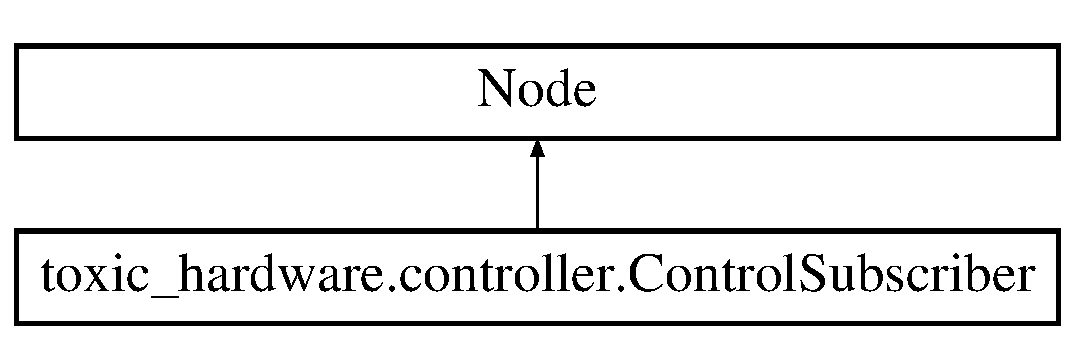
\includegraphics[height=2.000000cm]{d0/d16/classtoxic__hardware_1_1controller_1_1ControlSubscriber}
\end{center}
\end{figure}
\subsection*{Public Member Functions}
\begin{DoxyCompactItemize}
\item 
def \mbox{\hyperlink{classtoxic__hardware_1_1controller_1_1ControlSubscriber_ae64f0875afe3067b97ba370b354b9213}{\+\_\+\+\_\+init\+\_\+\+\_\+}} (self)
\item 
def \mbox{\hyperlink{classtoxic__hardware_1_1controller_1_1ControlSubscriber_a33e86027586e42bbaff819e19bef44d7}{control\+\_\+callback}} (self, data)
\end{DoxyCompactItemize}
\subsection*{Public Attributes}
\begin{DoxyCompactItemize}
\item 
\mbox{\hyperlink{classtoxic__hardware_1_1controller_1_1ControlSubscriber_a4b0698733c4dfaffe8e2b4cd952b6f82}{subscription}}
\item 
\mbox{\hyperlink{classtoxic__hardware_1_1controller_1_1ControlSubscriber_a2c40ddb28f990d22e258f62732f23fa4}{speed\+\_\+publisher}}
\item 
\mbox{\hyperlink{classtoxic__hardware_1_1controller_1_1ControlSubscriber_a194634798f6a458c7f9750bcd232fbbc}{steering\+\_\+publisher}}
\end{DoxyCompactItemize}


\subsection{Constructor \& Destructor Documentation}
\mbox{\Hypertarget{classtoxic__hardware_1_1controller_1_1ControlSubscriber_ae64f0875afe3067b97ba370b354b9213}\label{classtoxic__hardware_1_1controller_1_1ControlSubscriber_ae64f0875afe3067b97ba370b354b9213}} 
\index{toxic\+\_\+hardware\+::controller\+::\+Control\+Subscriber@{toxic\+\_\+hardware\+::controller\+::\+Control\+Subscriber}!\+\_\+\+\_\+init\+\_\+\+\_\+@{\+\_\+\+\_\+init\+\_\+\+\_\+}}
\index{\+\_\+\+\_\+init\+\_\+\+\_\+@{\+\_\+\+\_\+init\+\_\+\+\_\+}!toxic\+\_\+hardware\+::controller\+::\+Control\+Subscriber@{toxic\+\_\+hardware\+::controller\+::\+Control\+Subscriber}}
\subsubsection{\texorpdfstring{\+\_\+\+\_\+init\+\_\+\+\_\+()}{\_\_init\_\_()}}
{\footnotesize\ttfamily def \+\_\+\+\_\+init\+\_\+\+\_\+ (\begin{DoxyParamCaption}\item[{}]{self }\end{DoxyParamCaption})}


\begin{DoxyCode}
17     \textcolor{keyword}{def }\_\_init\_\_(self):
18         super().\_\_init\_\_(\textcolor{stringliteral}{'control\_toxic\_subscriber'})
19         self.subscription = self.create\_subscription(
20                 Joy,
21                 \textcolor{stringliteral}{'/joy'},
22                 self.control\_callback,
23                 60
24                 )
25         self.speed\_publisher = self.create\_publisher(Float64, \textcolor{stringliteral}{'/speed'}, 60)
26         self.steering\_publisher = self.create\_publisher(Float64, \textcolor{stringliteral}{'/steering'}, 60)
27         self.subscription
28         self.steering\_publisher
29         self.speed\_publisher
30 
\end{DoxyCode}


\subsection{Member Function Documentation}
\mbox{\Hypertarget{classtoxic__hardware_1_1controller_1_1ControlSubscriber_a33e86027586e42bbaff819e19bef44d7}\label{classtoxic__hardware_1_1controller_1_1ControlSubscriber_a33e86027586e42bbaff819e19bef44d7}} 
\index{toxic\+\_\+hardware\+::controller\+::\+Control\+Subscriber@{toxic\+\_\+hardware\+::controller\+::\+Control\+Subscriber}!control\+\_\+callback@{control\+\_\+callback}}
\index{control\+\_\+callback@{control\+\_\+callback}!toxic\+\_\+hardware\+::controller\+::\+Control\+Subscriber@{toxic\+\_\+hardware\+::controller\+::\+Control\+Subscriber}}
\subsubsection{\texorpdfstring{control\+\_\+callback()}{control\_callback()}}
{\footnotesize\ttfamily def control\+\_\+callback (\begin{DoxyParamCaption}\item[{}]{self,  }\item[{}]{data }\end{DoxyParamCaption})}


\begin{DoxyCode}
31     \textcolor{keyword}{def }control\_callback(self, data):
32         normalized\_steering = data.axes[0]
33         normalized\_fw\_speed = data.axes[5]
34         normalized\_bw\_speed = data.axes[2]
35         print(normalized\_steering)
36         print(normalized\_fw\_speed)
37         self.steering\_publisher.publish(Float64(normalized\_steering))
38         self.speed\_publisher.publish(Float64(normalized\_fw\_speed + normalized\_bw\_speed))
39 
\end{DoxyCode}


\subsection{Member Data Documentation}
\mbox{\Hypertarget{classtoxic__hardware_1_1controller_1_1ControlSubscriber_a2c40ddb28f990d22e258f62732f23fa4}\label{classtoxic__hardware_1_1controller_1_1ControlSubscriber_a2c40ddb28f990d22e258f62732f23fa4}} 
\index{toxic\+\_\+hardware\+::controller\+::\+Control\+Subscriber@{toxic\+\_\+hardware\+::controller\+::\+Control\+Subscriber}!speed\+\_\+publisher@{speed\+\_\+publisher}}
\index{speed\+\_\+publisher@{speed\+\_\+publisher}!toxic\+\_\+hardware\+::controller\+::\+Control\+Subscriber@{toxic\+\_\+hardware\+::controller\+::\+Control\+Subscriber}}
\subsubsection{\texorpdfstring{speed\+\_\+publisher}{speed\_publisher}}
{\footnotesize\ttfamily speed\+\_\+publisher}

\mbox{\Hypertarget{classtoxic__hardware_1_1controller_1_1ControlSubscriber_a194634798f6a458c7f9750bcd232fbbc}\label{classtoxic__hardware_1_1controller_1_1ControlSubscriber_a194634798f6a458c7f9750bcd232fbbc}} 
\index{toxic\+\_\+hardware\+::controller\+::\+Control\+Subscriber@{toxic\+\_\+hardware\+::controller\+::\+Control\+Subscriber}!steering\+\_\+publisher@{steering\+\_\+publisher}}
\index{steering\+\_\+publisher@{steering\+\_\+publisher}!toxic\+\_\+hardware\+::controller\+::\+Control\+Subscriber@{toxic\+\_\+hardware\+::controller\+::\+Control\+Subscriber}}
\subsubsection{\texorpdfstring{steering\+\_\+publisher}{steering\_publisher}}
{\footnotesize\ttfamily steering\+\_\+publisher}

\mbox{\Hypertarget{classtoxic__hardware_1_1controller_1_1ControlSubscriber_a4b0698733c4dfaffe8e2b4cd952b6f82}\label{classtoxic__hardware_1_1controller_1_1ControlSubscriber_a4b0698733c4dfaffe8e2b4cd952b6f82}} 
\index{toxic\+\_\+hardware\+::controller\+::\+Control\+Subscriber@{toxic\+\_\+hardware\+::controller\+::\+Control\+Subscriber}!subscription@{subscription}}
\index{subscription@{subscription}!toxic\+\_\+hardware\+::controller\+::\+Control\+Subscriber@{toxic\+\_\+hardware\+::controller\+::\+Control\+Subscriber}}
\subsubsection{\texorpdfstring{subscription}{subscription}}
{\footnotesize\ttfamily subscription}



The documentation for this class was generated from the following file\+:\begin{DoxyCompactItemize}
\item 
main\+\_\+ws/src/toxic\+\_\+hardware/toxic\+\_\+hardware/\mbox{\hyperlink{controller_8py}{controller.\+py}}\end{DoxyCompactItemize}

\hypertarget{classtoxic__vision_1_1webcam__pub_1_1ImagePublisher}{}\section{Image\+Publisher Class Reference}
\label{classtoxic__vision_1_1webcam__pub_1_1ImagePublisher}\index{Image\+Publisher@{Image\+Publisher}}
Inheritance diagram for Image\+Publisher\+:\begin{figure}[H]
\begin{center}
\leavevmode
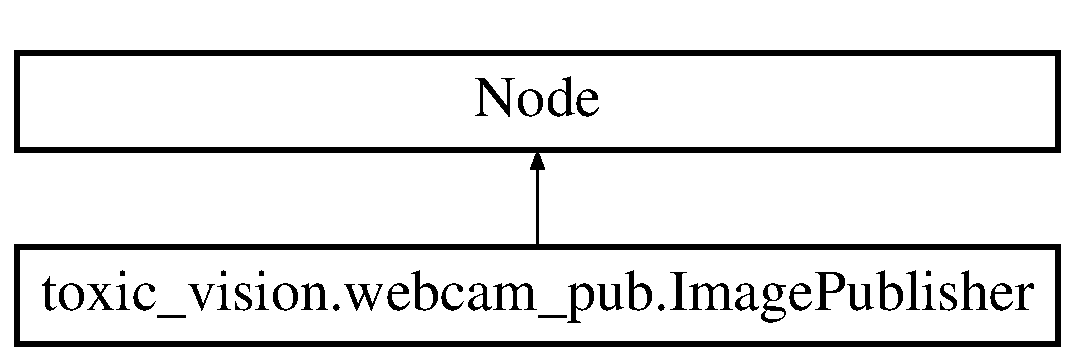
\includegraphics[height=2.000000cm]{d2/da6/classtoxic__vision_1_1webcam__pub_1_1ImagePublisher}
\end{center}
\end{figure}
\subsection*{Public Member Functions}
\begin{DoxyCompactItemize}
\item 
def \mbox{\hyperlink{classtoxic__vision_1_1webcam__pub_1_1ImagePublisher_ae64f0875afe3067b97ba370b354b9213}{\+\_\+\+\_\+init\+\_\+\+\_\+}} (self)
\begin{DoxyCompactList}\small\item\em \mbox{\hyperlink{classtoxic__vision_1_1webcam__pub_1_1ImagePublisher}{Image\+Publisher}} object to grab the live camera image and publish to a R\+O\+S2 Node as Cv\+Bridge message type. \end{DoxyCompactList}\item 
def \mbox{\hyperlink{classtoxic__vision_1_1webcam__pub_1_1ImagePublisher_a9692d7a212fa89bc61dacc687e826097}{timer\+\_\+callback}} (self)
\begin{DoxyCompactList}\small\item\em Timer callback to publish the image, everytime the timer achieve the desired time, this callback\textquotesingle{}ll run. \end{DoxyCompactList}\end{DoxyCompactItemize}
\subsection*{Public Attributes}
\begin{DoxyCompactItemize}
\item 
\mbox{\hyperlink{classtoxic__vision_1_1webcam__pub_1_1ImagePublisher_a2ab19359a5607f32a7b39d6d9f61c3b5}{publisher\+\_\+}}
\item 
\mbox{\hyperlink{classtoxic__vision_1_1webcam__pub_1_1ImagePublisher_a9fabcf6aa0647a2414f7cb1a2ab2634a}{timer}}
\item 
\mbox{\hyperlink{classtoxic__vision_1_1webcam__pub_1_1ImagePublisher_a9499a5c7f196d66c6afe0222bd5a9219}{cap}}
\item 
\mbox{\hyperlink{classtoxic__vision_1_1webcam__pub_1_1ImagePublisher_a88f0860257ba6bdc089557444f5cdd16}{br}}
\end{DoxyCompactItemize}


\subsection{Constructor \& Destructor Documentation}
\mbox{\Hypertarget{classtoxic__vision_1_1webcam__pub_1_1ImagePublisher_ae64f0875afe3067b97ba370b354b9213}\label{classtoxic__vision_1_1webcam__pub_1_1ImagePublisher_ae64f0875afe3067b97ba370b354b9213}} 
\index{toxic\+\_\+vision\+::webcam\+\_\+pub\+::\+Image\+Publisher@{toxic\+\_\+vision\+::webcam\+\_\+pub\+::\+Image\+Publisher}!\+\_\+\+\_\+init\+\_\+\+\_\+@{\+\_\+\+\_\+init\+\_\+\+\_\+}}
\index{\+\_\+\+\_\+init\+\_\+\+\_\+@{\+\_\+\+\_\+init\+\_\+\+\_\+}!toxic\+\_\+vision\+::webcam\+\_\+pub\+::\+Image\+Publisher@{toxic\+\_\+vision\+::webcam\+\_\+pub\+::\+Image\+Publisher}}
\subsubsection{\texorpdfstring{\+\_\+\+\_\+init\+\_\+\+\_\+()}{\_\_init\_\_()}}
{\footnotesize\ttfamily def \+\_\+\+\_\+init\+\_\+\+\_\+ (\begin{DoxyParamCaption}\item[{}]{self }\end{DoxyParamCaption})}



\mbox{\hyperlink{classtoxic__vision_1_1webcam__pub_1_1ImagePublisher}{Image\+Publisher}} object to grab the live camera image and publish to a R\+O\+S2 Node as Cv\+Bridge message type. 


\begin{DoxyParams}{Parameters}
{\em Node} & The R\+O\+S2 Node where the image publisher\textquotesingle{}ll be able to read/write (this time, just write)\\
\hline
\end{DoxyParams}
\begin{DoxyReturn}{Returns}
None, keeps running and alive while the camera\textquotesingle{}s oppened. \mbox{\hyperlink{classtoxic__vision_1_1webcam__pub_1_1ImagePublisher}{Image\+Publisher}} object init def (or constructor function, under a Java\textquotesingle{}s O\+OP context).
\end{DoxyReturn}

\begin{DoxyParams}{Parameters}
{\em self} & Self contained object like a \textquotesingle{}this\textquotesingle{} reference, just to read, write, and generally access object\textquotesingle{}s attributes.\\
\hline
\end{DoxyParams}
\begin{DoxyReturn}{Returns}
Image\+Publisher\+New\+Object returns a new image publisher object. 
\end{DoxyReturn}

\begin{DoxyCode}
65     \textcolor{keyword}{def }\_\_init\_\_(self):
66         
75 
76         \textcolor{comment}{# Edit source Node attributes.}
77         super().\_\_init\_\_(\textcolor{stringliteral}{'image\_publisher'}) \textcolor{comment}{# Edit source Node attributes.}
78         \textcolor{comment}{# Create the new publisher where the image'll published.}
79         self.publisher\_ = self.create\_publisher(Image, \textcolor{stringliteral}{'/raw\_rgb'}, 1)
80         \textcolor{comment}{# Something like 1/30 to achieve a FPS rate near to the 30FPS.}
81         timer\_period = 0.033
82         \textcolor{comment}{# Set and start running the timer.}
83         self.timer = self.create\_timer(timer\_period, self.timer\_callback)
84         \textcolor{comment}{# Open the webcam and store the object to interact as a VideoCapture}
85         \textcolor{comment}{# object}
86         self.cap = cv2.VideoCapture(0)
87         \textcolor{comment}{# Set the desired frame width}
88         self.cap.set(cv2.CAP\_PROP\_FRAME\_WIDTH, 640)
89         \textcolor{comment}{# Set the desired frame height}
90         self.cap.set(cv2.CAP\_PROP\_FRAME\_HEIGHT, 480)
91         \textcolor{comment}{# Set the desired framerate}
92         self.cap.set(cv2.CAP\_PROP\_FPS, 30)
93         \textcolor{comment}{# Create the Ros2 to OpenCv Bridge}
94         self.br = CvBridge()
95 
\end{DoxyCode}


\subsection{Member Function Documentation}
\mbox{\Hypertarget{classtoxic__vision_1_1webcam__pub_1_1ImagePublisher_a9692d7a212fa89bc61dacc687e826097}\label{classtoxic__vision_1_1webcam__pub_1_1ImagePublisher_a9692d7a212fa89bc61dacc687e826097}} 
\index{toxic\+\_\+vision\+::webcam\+\_\+pub\+::\+Image\+Publisher@{toxic\+\_\+vision\+::webcam\+\_\+pub\+::\+Image\+Publisher}!timer\+\_\+callback@{timer\+\_\+callback}}
\index{timer\+\_\+callback@{timer\+\_\+callback}!toxic\+\_\+vision\+::webcam\+\_\+pub\+::\+Image\+Publisher@{toxic\+\_\+vision\+::webcam\+\_\+pub\+::\+Image\+Publisher}}
\subsubsection{\texorpdfstring{timer\+\_\+callback()}{timer\_callback()}}
{\footnotesize\ttfamily def timer\+\_\+callback (\begin{DoxyParamCaption}\item[{}]{self }\end{DoxyParamCaption})}



Timer callback to publish the image, everytime the timer achieve the desired time, this callback\textquotesingle{}ll run. 


\begin{DoxyParams}{Parameters}
{\em self} & Self contained object like a \textquotesingle{}this\textquotesingle{} reference, jus to read, write, and generally access object\textquotesingle{}s attributes.\\
\hline
\end{DoxyParams}
\begin{DoxyReturn}{Returns}
None, just publish the current frame. 
\end{DoxyReturn}

\begin{DoxyCode}
96     \textcolor{keyword}{def }timer\_callback(self):
97         
106 
107         \textcolor{comment}{# Read the current frame.}
108         ret, frame = self.cap.read()
109         \textcolor{comment}{# Validate there's a new image}
110         \textcolor{keywordflow}{if} ret:
111             \textcolor{comment}{# If there's a new image, parse the frame to ROS2 image message}
112             \textcolor{comment}{# type and publish to the node}
113             self.publisher\_.publish(self.br.cv2\_to\_imgmsg(frame))
114 
\end{DoxyCode}


\subsection{Member Data Documentation}
\mbox{\Hypertarget{classtoxic__vision_1_1webcam__pub_1_1ImagePublisher_a88f0860257ba6bdc089557444f5cdd16}\label{classtoxic__vision_1_1webcam__pub_1_1ImagePublisher_a88f0860257ba6bdc089557444f5cdd16}} 
\index{toxic\+\_\+vision\+::webcam\+\_\+pub\+::\+Image\+Publisher@{toxic\+\_\+vision\+::webcam\+\_\+pub\+::\+Image\+Publisher}!br@{br}}
\index{br@{br}!toxic\+\_\+vision\+::webcam\+\_\+pub\+::\+Image\+Publisher@{toxic\+\_\+vision\+::webcam\+\_\+pub\+::\+Image\+Publisher}}
\subsubsection{\texorpdfstring{br}{br}}
{\footnotesize\ttfamily br}

\mbox{\Hypertarget{classtoxic__vision_1_1webcam__pub_1_1ImagePublisher_a9499a5c7f196d66c6afe0222bd5a9219}\label{classtoxic__vision_1_1webcam__pub_1_1ImagePublisher_a9499a5c7f196d66c6afe0222bd5a9219}} 
\index{toxic\+\_\+vision\+::webcam\+\_\+pub\+::\+Image\+Publisher@{toxic\+\_\+vision\+::webcam\+\_\+pub\+::\+Image\+Publisher}!cap@{cap}}
\index{cap@{cap}!toxic\+\_\+vision\+::webcam\+\_\+pub\+::\+Image\+Publisher@{toxic\+\_\+vision\+::webcam\+\_\+pub\+::\+Image\+Publisher}}
\subsubsection{\texorpdfstring{cap}{cap}}
{\footnotesize\ttfamily cap}

\mbox{\Hypertarget{classtoxic__vision_1_1webcam__pub_1_1ImagePublisher_a2ab19359a5607f32a7b39d6d9f61c3b5}\label{classtoxic__vision_1_1webcam__pub_1_1ImagePublisher_a2ab19359a5607f32a7b39d6d9f61c3b5}} 
\index{toxic\+\_\+vision\+::webcam\+\_\+pub\+::\+Image\+Publisher@{toxic\+\_\+vision\+::webcam\+\_\+pub\+::\+Image\+Publisher}!publisher\+\_\+@{publisher\+\_\+}}
\index{publisher\+\_\+@{publisher\+\_\+}!toxic\+\_\+vision\+::webcam\+\_\+pub\+::\+Image\+Publisher@{toxic\+\_\+vision\+::webcam\+\_\+pub\+::\+Image\+Publisher}}
\subsubsection{\texorpdfstring{publisher\+\_\+}{publisher\_}}
{\footnotesize\ttfamily publisher\+\_\+}

\mbox{\Hypertarget{classtoxic__vision_1_1webcam__pub_1_1ImagePublisher_a9fabcf6aa0647a2414f7cb1a2ab2634a}\label{classtoxic__vision_1_1webcam__pub_1_1ImagePublisher_a9fabcf6aa0647a2414f7cb1a2ab2634a}} 
\index{toxic\+\_\+vision\+::webcam\+\_\+pub\+::\+Image\+Publisher@{toxic\+\_\+vision\+::webcam\+\_\+pub\+::\+Image\+Publisher}!timer@{timer}}
\index{timer@{timer}!toxic\+\_\+vision\+::webcam\+\_\+pub\+::\+Image\+Publisher@{toxic\+\_\+vision\+::webcam\+\_\+pub\+::\+Image\+Publisher}}
\subsubsection{\texorpdfstring{timer}{timer}}
{\footnotesize\ttfamily timer}



The documentation for this class was generated from the following file\+:\begin{DoxyCompactItemize}
\item 
main\+\_\+ws/src/toxic\+\_\+vision/toxic\+\_\+vision/\mbox{\hyperlink{webcam__pub_8py}{webcam\+\_\+pub.\+py}}\end{DoxyCompactItemize}

\hypertarget{classtoxic__vision_1_1lane__detector_1_1ImageSubscriber}{}\doxysection{Image\+Subscriber Class Reference}
\label{classtoxic__vision_1_1lane__detector_1_1ImageSubscriber}\index{ImageSubscriber@{ImageSubscriber}}
Inheritance diagram for Image\+Subscriber\+:\begin{figure}[H]
\begin{center}
\leavevmode
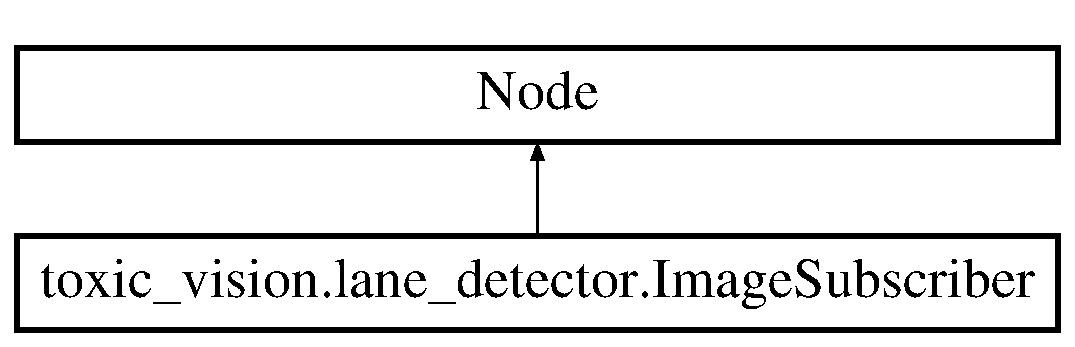
\includegraphics[height=2.000000cm]{d8/d32/classtoxic__vision_1_1lane__detector_1_1ImageSubscriber}
\end{center}
\end{figure}
\doxysubsection*{Public Member Functions}
\begin{DoxyCompactItemize}
\item 
def \mbox{\hyperlink{classtoxic__vision_1_1lane__detector_1_1ImageSubscriber_ae64f0875afe3067b97ba370b354b9213}{\+\_\+\+\_\+init\+\_\+\+\_\+}} (self)
\item 
def \mbox{\hyperlink{classtoxic__vision_1_1lane__detector_1_1ImageSubscriber_a876735be946e8770790a53a398cbab17}{range\+\_\+finder}} (self)
\item 
def \mbox{\hyperlink{classtoxic__vision_1_1lane__detector_1_1ImageSubscriber_a69f776519af775d0e6b8ef2bf9b2a37f}{process\+\_\+image}} (self)
\item 
def \mbox{\hyperlink{classtoxic__vision_1_1lane__detector_1_1ImageSubscriber_aa29031ea99aa06784e3755c54ba91edd}{two\+\_\+dots\+\_\+line}} (self, rho, theta, \mbox{\hyperlink{namespacetoxic__vision_1_1lane__detector_a9c845a56c4d49b65dea74d4e4f9df6d1}{frame}})
\item 
def \mbox{\hyperlink{classtoxic__vision_1_1lane__detector_1_1ImageSubscriber_ad3a1feb0c65612f560e670f5f064de28}{line\+\_\+finder}} (self)
\item 
def \mbox{\hyperlink{classtoxic__vision_1_1lane__detector_1_1ImageSubscriber_a23dd9943cb7cb7be2a6e7022a85a1684}{listener\+\_\+callback}} (self, data)
\end{DoxyCompactItemize}
\doxysubsection*{Public Attributes}
\begin{DoxyCompactItemize}
\item 
\mbox{\hyperlink{classtoxic__vision_1_1lane__detector_1_1ImageSubscriber_a4b0698733c4dfaffe8e2b4cd952b6f82}{subscription}}
\item 
\mbox{\hyperlink{classtoxic__vision_1_1lane__detector_1_1ImageSubscriber_a23e707c10db59b59318fc639544333c0}{left\+\_\+lane\+\_\+publisher}}
\item 
\mbox{\hyperlink{classtoxic__vision_1_1lane__detector_1_1ImageSubscriber_ad43f05368e8ce07fbadd327fe8e2b9bf}{right\+\_\+lane\+\_\+publisher}}
\item 
\mbox{\hyperlink{classtoxic__vision_1_1lane__detector_1_1ImageSubscriber_a88f0860257ba6bdc089557444f5cdd16}{br}}
\end{DoxyCompactItemize}


\doxysubsection{Constructor \& Destructor Documentation}
\mbox{\Hypertarget{classtoxic__vision_1_1lane__detector_1_1ImageSubscriber_ae64f0875afe3067b97ba370b354b9213}\label{classtoxic__vision_1_1lane__detector_1_1ImageSubscriber_ae64f0875afe3067b97ba370b354b9213}} 
\index{ImageSubscriber@{ImageSubscriber}!\_\_init\_\_@{\_\_init\_\_}}
\index{\_\_init\_\_@{\_\_init\_\_}!ImageSubscriber@{ImageSubscriber}}
\doxysubsubsection{\texorpdfstring{\_\_init\_\_()}{\_\_init\_\_()}}
{\footnotesize\ttfamily def \+\_\+\+\_\+init\+\_\+\+\_\+ (\begin{DoxyParamCaption}\item[{}]{self }\end{DoxyParamCaption})}


\begin{DoxyCode}{0}
\DoxyCodeLine{95   \textcolor{keyword}{def }\_\_init\_\_(self):}
\DoxyCodeLine{96     super().\_\_init\_\_(\textcolor{stringliteral}{'image\_subscriber'})}
\DoxyCodeLine{97     self.subscription = self.create\_subscription(}
\DoxyCodeLine{98       Image, }
\DoxyCodeLine{99       \textcolor{stringliteral}{'/raw\_rgb'}, }
\DoxyCodeLine{100       self.listener\_callback, }
\DoxyCodeLine{101       1}
\DoxyCodeLine{102       )}
\DoxyCodeLine{103     self.left\_lane\_publisher = self.create\_publisher(Float64MultiArray, \textcolor{stringliteral}{'/lines/left'}, 1)}
\DoxyCodeLine{104     self.right\_lane\_publisher = self.create\_publisher(Float64MultiArray, \textcolor{stringliteral}{'/lines/right'}, 1)}
\DoxyCodeLine{105     self.subscription}
\DoxyCodeLine{106     self.br = CvBridge()}
\DoxyCodeLine{107     \textcolor{comment}{\# \}\}\}}}
\DoxyCodeLine{108 }

\end{DoxyCode}


\doxysubsection{Member Function Documentation}
\mbox{\Hypertarget{classtoxic__vision_1_1lane__detector_1_1ImageSubscriber_ad3a1feb0c65612f560e670f5f064de28}\label{classtoxic__vision_1_1lane__detector_1_1ImageSubscriber_ad3a1feb0c65612f560e670f5f064de28}} 
\index{ImageSubscriber@{ImageSubscriber}!line\_finder@{line\_finder}}
\index{line\_finder@{line\_finder}!ImageSubscriber@{ImageSubscriber}}
\doxysubsubsection{\texorpdfstring{line\_finder()}{line\_finder()}}
{\footnotesize\ttfamily def line\+\_\+finder (\begin{DoxyParamCaption}\item[{}]{self }\end{DoxyParamCaption})}


\begin{DoxyCode}{0}
\DoxyCodeLine{142   \textcolor{keyword}{def }line\_finder(self):}
\DoxyCodeLine{143       \textcolor{keyword}{global} band\_pass, frame, dst}
\DoxyCodeLine{144       \textcolor{keyword}{global} right\_theta\_min, right\_theta\_max, right\_rho\_min, right\_rho\_max}
\DoxyCodeLine{145       \textcolor{keyword}{global} left\_theta\_min, left\_theta\_max, left\_rho\_min, left\_rho\_max}
\DoxyCodeLine{146       \textcolor{keyword}{global} lower, upper, lefter, righter, upper\_color, lower\_color, color\_delta}
\DoxyCodeLine{147       \textcolor{keyword}{global} average\_rho\_left, average\_rho\_right, average\_theta\_left, average\_theta\_right}
\DoxyCodeLine{148       kernel = np.ones((6, 6), np.uint8) }
\DoxyCodeLine{149       band\_pass = cv2.morphologyEx(band\_pass, cv2.MORPH\_OPEN, kernel, iterations=1)}
\DoxyCodeLine{150       dst = cv2.Canny(band\_pass, 100, 100, 10, \textcolor{keywordtype}{None})}
\DoxyCodeLine{151       lines = cv2.HoughLinesP(dst, 3, np.pi/90, 80, minLineLength=25, maxLineGap=1)}
\DoxyCodeLine{152       \textcolor{keywordflow}{if} lines \textcolor{keywordflow}{is} \textcolor{keywordflow}{not} \textcolor{keywordtype}{None}:}
\DoxyCodeLine{153           lines = lines[:, 0]}
\DoxyCodeLine{154       \textcolor{keywordflow}{if} lines \textcolor{keywordflow}{is} \textcolor{keywordflow}{not} \textcolor{keywordtype}{None}:}
\DoxyCodeLine{155           sum\_theta\_left = 0}
\DoxyCodeLine{156           sum\_rho\_left = 0}
\DoxyCodeLine{157           sum\_theta\_right = 0}
\DoxyCodeLine{158           sum\_rho\_right = 0}
\DoxyCodeLine{159           count\_left = 0}
\DoxyCodeLine{160           count\_right = 0}
\DoxyCodeLine{161           h = 0}
\DoxyCodeLine{162           s = 0}
\DoxyCodeLine{163           counter\_color = 0}
\DoxyCodeLine{164           \textcolor{keywordflow}{for} i \textcolor{keywordflow}{in} range(0, len(lines)):}
\DoxyCodeLine{165               l = lines[i]}
\DoxyCodeLine{166               rho, theta = \mbox{\hyperlink{namespacetoxic__vision_1_1lane__detector_ae3bdbfab97718df7c906f65d19f10dfd}{to\_normal\_form}}(l[0], l[1], l[2], l[3])}
\DoxyCodeLine{167               \textcolor{keywordflow}{if} (average\_rho\_right == 0}
\DoxyCodeLine{168                   \textcolor{keywordflow}{and} average\_theta\_right == 0}
\DoxyCodeLine{169                   \textcolor{keywordflow}{and} (}
\DoxyCodeLine{170                       (}
\DoxyCodeLine{171                           (}
\DoxyCodeLine{172                               (450 <= l[0] <= 590)}
\DoxyCodeLine{173                               \textcolor{keywordflow}{and} (140 <= l[1] <= 240)}
\DoxyCodeLine{174                           )}
\DoxyCodeLine{175                           \textcolor{keywordflow}{or} (}
\DoxyCodeLine{176                               (450 <= l[2] <= 590)}
\DoxyCodeLine{177                               \textcolor{keywordflow}{and} (140 <= l[3] <= 240)}
\DoxyCodeLine{178                              )}
\DoxyCodeLine{179                      )}
\DoxyCodeLine{180                   )}
\DoxyCodeLine{181                  ):}
\DoxyCodeLine{182                   sum\_theta\_right += theta}
\DoxyCodeLine{183                   sum\_rho\_right += rho}
\DoxyCodeLine{184                   count\_right += 1}
\DoxyCodeLine{185               \textcolor{keywordflow}{elif} (average\_rho\_left == 0}
\DoxyCodeLine{186                     \textcolor{keywordflow}{and} average\_theta\_left == 0}
\DoxyCodeLine{187                   \textcolor{keywordflow}{and} (}
\DoxyCodeLine{188                       (}
\DoxyCodeLine{189                           (}
\DoxyCodeLine{190                               (50 <= l[0] <= 190)}
\DoxyCodeLine{191                               \textcolor{keywordflow}{and} (140 <= l[1] <= 240)}
\DoxyCodeLine{192                           )}
\DoxyCodeLine{193                           \textcolor{keywordflow}{or} (}
\DoxyCodeLine{194                               (50 <= l[2] <= 190)}
\DoxyCodeLine{195                               \textcolor{keywordflow}{and} (140 <= l[3] <= 240)}
\DoxyCodeLine{196                              )}
\DoxyCodeLine{197                      )}
\DoxyCodeLine{198                   )}
\DoxyCodeLine{199                 ):}
\DoxyCodeLine{200                   sum\_theta\_left += theta}
\DoxyCodeLine{201                   sum\_rho\_left += rho}
\DoxyCodeLine{202                   count\_left += 1}
\DoxyCodeLine{203               \textcolor{keywordflow}{elif} (}
\DoxyCodeLine{204                       (right\_theta\_min <= theta <= right\_theta\_max)}
\DoxyCodeLine{205                       \textcolor{keywordflow}{and} (right\_rho\_min <= rho <= right\_rho\_max)}
\DoxyCodeLine{206                  ):}
\DoxyCodeLine{207                   sum\_theta\_right += theta}
\DoxyCodeLine{208                   sum\_rho\_right += rho}
\DoxyCodeLine{209                   count\_right += 1}
\DoxyCodeLine{210                   print(\textcolor{stringliteral}{"{}rho:\{\}\(\backslash\)ttheta:\{\}\(\backslash\)tpassed as right"{}}.format(}
\DoxyCodeLine{211                       rho,}
\DoxyCodeLine{212                       theta}
\DoxyCodeLine{213                       ))}
\DoxyCodeLine{214               \textcolor{keywordflow}{elif} (}
\DoxyCodeLine{215                       (left\_theta\_min <= theta <= left\_theta\_max)}
\DoxyCodeLine{216                       \textcolor{keywordflow}{and} (left\_rho\_min <= rho <= left\_rho\_max)}
\DoxyCodeLine{217                    ):}
\DoxyCodeLine{218                   sum\_theta\_left += theta}
\DoxyCodeLine{219                   sum\_rho\_left += rho}
\DoxyCodeLine{220                   count\_left += 1}
\DoxyCodeLine{221                   \textcolor{stringliteral}{"{}"{}"{}}}
\DoxyCodeLine{222 \textcolor{stringliteral}{                  print("{}rho:\{\}\(\backslash\)ttheta:\{\}\(\backslash\)tpassed as left"{}.format(}}
\DoxyCodeLine{223 \textcolor{stringliteral}{                      rho,}}
\DoxyCodeLine{224 \textcolor{stringliteral}{                      theta}}
\DoxyCodeLine{225 \textcolor{stringliteral}{                      ))}}
\DoxyCodeLine{226 \textcolor{stringliteral}{                  "{}"{}"{}}}
\DoxyCodeLine{227               \textcolor{keywordflow}{else}:}
\DoxyCodeLine{228                   if(theta > 0):}
\DoxyCodeLine{229                       cv2.line(frame, (l[0], l[1]), (l[2], l[3]), (255,255,0), 3, cv2.LINE\_AA)}
\DoxyCodeLine{230                       \textcolor{comment}{\#print("{}\{\} > 0"{}.format(theta))}}
\DoxyCodeLine{231                   elif(theta < 0):}
\DoxyCodeLine{232                       cv2.line(frame, (l[0], l[1]), (l[2], l[3]), (0,255,255), 3, cv2.LINE\_AA)}
\DoxyCodeLine{233                       print([right\_theta\_min, theta, right\_theta\_max])}
\DoxyCodeLine{234                       print([right\_rho\_min, rho, right\_rho\_max])}
\DoxyCodeLine{235           \textcolor{keywordflow}{if} count\_left > 0:}
\DoxyCodeLine{236               \textcolor{comment}{\#print("{}count\_left is bigger than zero"{})}}
\DoxyCodeLine{237               average\_rho\_left = sum\_rho\_left / count\_left}
\DoxyCodeLine{238               average\_theta\_left = sum\_theta\_left / count\_left}
\DoxyCodeLine{239               left\_theta\_min = average\_theta\_left -\/ variance\_theta}
\DoxyCodeLine{240               left\_theta\_max = average\_theta\_left + variance\_theta}
\DoxyCodeLine{241               left\_rho\_min = average\_rho\_left -\/ variance\_rho}
\DoxyCodeLine{242               left\_rho\_max = average\_rho\_left + variance\_rho}
\DoxyCodeLine{243               message = Float64MultiArray()}
\DoxyCodeLine{244               message.data = [average\_rho\_left, average\_theta\_left]}
\DoxyCodeLine{245               self.left\_lane\_publisher.publish(message)}
\DoxyCodeLine{246               \textcolor{comment}{\#print([left\_rho\_min, average\_rho\_left, left\_rho\_max])}}
\DoxyCodeLine{247               \textcolor{comment}{\#print([left\_theta\_min, average\_theta\_left, left\_theta\_max])}}
\DoxyCodeLine{248               \textcolor{comment}{\#"{}"{}"{}}}
\DoxyCodeLine{249               \textcolor{keywordflow}{try}:}
\DoxyCodeLine{250                   x1, y1, x2, y2 = self.two\_dots\_line(average\_rho\_left, average\_theta\_left, frame)}
\DoxyCodeLine{251                   x3 = x1 + delta}
\DoxyCodeLine{252                   x4 = x1 -\/ delta}
\DoxyCodeLine{253                   x5 = x2 + delta}
\DoxyCodeLine{254                   x6 = x2 -\/ delta}
\DoxyCodeLine{255                   cv2.line(frame, (x1, y1), (x2, y2), (255,0,0), 3, cv2.LINE\_AA)}
\DoxyCodeLine{256               \textcolor{keywordflow}{except}:}
\DoxyCodeLine{257                   \textcolor{keywordflow}{pass}}
\DoxyCodeLine{258               \textcolor{comment}{\#"{}"{}"{}}}
\DoxyCodeLine{259           \textcolor{keywordflow}{if} count\_right > 0:}
\DoxyCodeLine{260               print(\textcolor{stringliteral}{"{}count\_right is bigger than zero"{}})}
\DoxyCodeLine{261               average\_rho\_right = sum\_rho\_right / count\_right}
\DoxyCodeLine{262               average\_theta\_right = sum\_theta\_right / count\_right}
\DoxyCodeLine{263               right\_theta\_min = average\_theta\_right -\/ variance\_theta}
\DoxyCodeLine{264               right\_theta\_max = average\_theta\_right + variance\_theta}
\DoxyCodeLine{265               right\_rho\_min = average\_rho\_right -\/ variance\_rho}
\DoxyCodeLine{266               right\_rho\_max = average\_rho\_right + variance\_rho}
\DoxyCodeLine{267               message = Float64MultiArray()}
\DoxyCodeLine{268               message.data = [average\_rho\_right, average\_theta\_right]}
\DoxyCodeLine{269               self.right\_lane\_publisher.publish(message)}
\DoxyCodeLine{270               print([right\_rho\_min, average\_rho\_right, right\_rho\_max])}
\DoxyCodeLine{271               print([right\_theta\_min, average\_theta\_right, right\_theta\_max])}
\DoxyCodeLine{272               \textcolor{comment}{\#"{}"{}"{}}}
\DoxyCodeLine{273               \textcolor{keywordflow}{try}:}
\DoxyCodeLine{274                   x1, y1, x2, y2 = self.two\_dots\_line(average\_rho\_right, average\_theta\_right, frame)}
\DoxyCodeLine{275                   x3 = x1 + delta}
\DoxyCodeLine{276                   x4 = x1 -\/ delta}
\DoxyCodeLine{277                   x5 = x2 + delta}
\DoxyCodeLine{278                   x6 = x2 -\/ delta}
\DoxyCodeLine{279                   cv2.line(frame, (x1, y1), (x2, y2), (0,0,255), 3, cv2.LINE\_AA)}
\DoxyCodeLine{280               \textcolor{keywordflow}{except} Exception \textcolor{keyword}{as} e:}
\DoxyCodeLine{281                   print(e)}
\DoxyCodeLine{282               \textcolor{comment}{\#"{}"{}"{}}}
\DoxyCodeLine{283           frame = cv2.rectangle(frame, (50, 140), (190, 240), (255, 0, 0), 5)}
\DoxyCodeLine{284           frame = cv2.rectangle(frame, (450, 140), (590, 240), (0, 0, 255), 5)}
\DoxyCodeLine{285           \textcolor{comment}{\#print("{}\#\#\#\#\#\#\#\#\#\#\#\#\#\#\#\#\#\#\#\#\#\#\#\#\#\#\#\#\#\#\#\#\#\#\#\#\#\#\#\#\#\#\#\#\#\#\#\#\#\#\#\#\#\#\#\#\#\#\#\#\#"{})}}

\end{DoxyCode}
\mbox{\Hypertarget{classtoxic__vision_1_1lane__detector_1_1ImageSubscriber_a23dd9943cb7cb7be2a6e7022a85a1684}\label{classtoxic__vision_1_1lane__detector_1_1ImageSubscriber_a23dd9943cb7cb7be2a6e7022a85a1684}} 
\index{ImageSubscriber@{ImageSubscriber}!listener\_callback@{listener\_callback}}
\index{listener\_callback@{listener\_callback}!ImageSubscriber@{ImageSubscriber}}
\doxysubsubsection{\texorpdfstring{listener\_callback()}{listener\_callback()}}
{\footnotesize\ttfamily def listener\+\_\+callback (\begin{DoxyParamCaption}\item[{}]{self,  }\item[{}]{data }\end{DoxyParamCaption})}


\begin{DoxyCode}{0}
\DoxyCodeLine{289   \textcolor{keyword}{def }listener\_callback(self, data):}
\DoxyCodeLine{290     \textcolor{keyword}{global} frame, band\_pass, dst}
\DoxyCodeLine{291     frame = self.br.imgmsg\_to\_cv2(data)[240:, :, :]}
\DoxyCodeLine{292     \textcolor{comment}{\#frame = current\_frame}}
\DoxyCodeLine{293     hsv = self.process\_image()}
\DoxyCodeLine{294     band\_pass = self.range\_finder()}
\DoxyCodeLine{295     self.line\_finder()}
\DoxyCodeLine{296     \textcolor{comment}{\#"{}"{}"{}}}
\DoxyCodeLine{297     cv2.imshow(\textcolor{stringliteral}{"{}camera"{}}, frame)}
\DoxyCodeLine{298     cv2.imshow(\textcolor{stringliteral}{"{}band\_filter"{}}, band\_pass)}
\DoxyCodeLine{299     cv2.imshow(\textcolor{stringliteral}{"{}dst"{}}, dst)}
\DoxyCodeLine{300     cv2.setMouseCallback(\textcolor{stringliteral}{"{}camera"{}}, mouse\_callback)}
\DoxyCodeLine{301     cv2.setMouseCallback(\textcolor{stringliteral}{"{}dst"{}}, mouse\_callback)}
\DoxyCodeLine{302     cv2.setMouseCallback(\textcolor{stringliteral}{"{}band\_filter"{}}, mouse\_callback)}
\DoxyCodeLine{303     cv2.waitKey(1)}
\DoxyCodeLine{304     \textcolor{comment}{\#"{}"{}"{}}}

\end{DoxyCode}
\mbox{\Hypertarget{classtoxic__vision_1_1lane__detector_1_1ImageSubscriber_a69f776519af775d0e6b8ef2bf9b2a37f}\label{classtoxic__vision_1_1lane__detector_1_1ImageSubscriber_a69f776519af775d0e6b8ef2bf9b2a37f}} 
\index{ImageSubscriber@{ImageSubscriber}!process\_image@{process\_image}}
\index{process\_image@{process\_image}!ImageSubscriber@{ImageSubscriber}}
\doxysubsubsection{\texorpdfstring{process\_image()}{process\_image()}}
{\footnotesize\ttfamily def process\+\_\+image (\begin{DoxyParamCaption}\item[{}]{self }\end{DoxyParamCaption})}


\begin{DoxyCode}{0}
\DoxyCodeLine{121   \textcolor{keyword}{def }process\_image(self):}
\DoxyCodeLine{122       \textcolor{keyword}{global} frame, where}
\DoxyCodeLine{123       hsv = cv2.cvtColor(frame, cv2.COLOR\_BGR2HLS)}
\DoxyCodeLine{124       where = hsv}
\DoxyCodeLine{125       \textcolor{keywordflow}{return} hsv}

\end{DoxyCode}
\mbox{\Hypertarget{classtoxic__vision_1_1lane__detector_1_1ImageSubscriber_a876735be946e8770790a53a398cbab17}\label{classtoxic__vision_1_1lane__detector_1_1ImageSubscriber_a876735be946e8770790a53a398cbab17}} 
\index{ImageSubscriber@{ImageSubscriber}!range\_finder@{range\_finder}}
\index{range\_finder@{range\_finder}!ImageSubscriber@{ImageSubscriber}}
\doxysubsubsection{\texorpdfstring{range\_finder()}{range\_finder()}}
{\footnotesize\ttfamily def range\+\_\+finder (\begin{DoxyParamCaption}\item[{}]{self }\end{DoxyParamCaption})}


\begin{DoxyCode}{0}
\DoxyCodeLine{110   \textcolor{keyword}{def }range\_finder(self):}
\DoxyCodeLine{111     \textcolor{keyword}{global} lower\_color, upper\_color, where}
\DoxyCodeLine{112     band\_filter = cv2.inRange(}
\DoxyCodeLine{113                 where,}
\DoxyCodeLine{114             np.array(lower\_color),}
\DoxyCodeLine{115             np.array(upper\_color)}
\DoxyCodeLine{116         )}
\DoxyCodeLine{117     \textcolor{keywordflow}{return} band\_filter}

\end{DoxyCode}
\mbox{\Hypertarget{classtoxic__vision_1_1lane__detector_1_1ImageSubscriber_aa29031ea99aa06784e3755c54ba91edd}\label{classtoxic__vision_1_1lane__detector_1_1ImageSubscriber_aa29031ea99aa06784e3755c54ba91edd}} 
\index{ImageSubscriber@{ImageSubscriber}!two\_dots\_line@{two\_dots\_line}}
\index{two\_dots\_line@{two\_dots\_line}!ImageSubscriber@{ImageSubscriber}}
\doxysubsubsection{\texorpdfstring{two\_dots\_line()}{two\_dots\_line()}}
{\footnotesize\ttfamily def two\+\_\+dots\+\_\+line (\begin{DoxyParamCaption}\item[{}]{self,  }\item[{}]{rho,  }\item[{}]{theta,  }\item[{}]{frame }\end{DoxyParamCaption})}


\begin{DoxyCode}{0}
\DoxyCodeLine{129   \textcolor{keyword}{def }two\_dots\_line(self, rho, theta, frame):}
\DoxyCodeLine{130       \textcolor{keywordflow}{if} rho == 0 \textcolor{keywordflow}{or} theta == 0:}
\DoxyCodeLine{131           \textcolor{keywordflow}{return}}
\DoxyCodeLine{132       a = math.cos(theta)}
\DoxyCodeLine{133       b = math.sin(theta)}
\DoxyCodeLine{134       x0 = a * rho}
\DoxyCodeLine{135       y0 = b * rho}
\DoxyCodeLine{136       pt1 = (int(x0 + 1000*(-\/b)), int(y0 + 1000*(a)))}
\DoxyCodeLine{137       pt2 = (int(x0 -\/ 1000*(-\/b)), int(y0 -\/ 1000*(a)))}
\DoxyCodeLine{138       \textcolor{keywordflow}{return} pt1[0], pt1[1], pt2[0], pt2[1]}

\end{DoxyCode}


\doxysubsection{Member Data Documentation}
\mbox{\Hypertarget{classtoxic__vision_1_1lane__detector_1_1ImageSubscriber_a88f0860257ba6bdc089557444f5cdd16}\label{classtoxic__vision_1_1lane__detector_1_1ImageSubscriber_a88f0860257ba6bdc089557444f5cdd16}} 
\index{ImageSubscriber@{ImageSubscriber}!br@{br}}
\index{br@{br}!ImageSubscriber@{ImageSubscriber}}
\doxysubsubsection{\texorpdfstring{br}{br}}
{\footnotesize\ttfamily br}

\mbox{\Hypertarget{classtoxic__vision_1_1lane__detector_1_1ImageSubscriber_a23e707c10db59b59318fc639544333c0}\label{classtoxic__vision_1_1lane__detector_1_1ImageSubscriber_a23e707c10db59b59318fc639544333c0}} 
\index{ImageSubscriber@{ImageSubscriber}!left\_lane\_publisher@{left\_lane\_publisher}}
\index{left\_lane\_publisher@{left\_lane\_publisher}!ImageSubscriber@{ImageSubscriber}}
\doxysubsubsection{\texorpdfstring{left\_lane\_publisher}{left\_lane\_publisher}}
{\footnotesize\ttfamily left\+\_\+lane\+\_\+publisher}

\mbox{\Hypertarget{classtoxic__vision_1_1lane__detector_1_1ImageSubscriber_ad43f05368e8ce07fbadd327fe8e2b9bf}\label{classtoxic__vision_1_1lane__detector_1_1ImageSubscriber_ad43f05368e8ce07fbadd327fe8e2b9bf}} 
\index{ImageSubscriber@{ImageSubscriber}!right\_lane\_publisher@{right\_lane\_publisher}}
\index{right\_lane\_publisher@{right\_lane\_publisher}!ImageSubscriber@{ImageSubscriber}}
\doxysubsubsection{\texorpdfstring{right\_lane\_publisher}{right\_lane\_publisher}}
{\footnotesize\ttfamily right\+\_\+lane\+\_\+publisher}

\mbox{\Hypertarget{classtoxic__vision_1_1lane__detector_1_1ImageSubscriber_a4b0698733c4dfaffe8e2b4cd952b6f82}\label{classtoxic__vision_1_1lane__detector_1_1ImageSubscriber_a4b0698733c4dfaffe8e2b4cd952b6f82}} 
\index{ImageSubscriber@{ImageSubscriber}!subscription@{subscription}}
\index{subscription@{subscription}!ImageSubscriber@{ImageSubscriber}}
\doxysubsubsection{\texorpdfstring{subscription}{subscription}}
{\footnotesize\ttfamily subscription}



The documentation for this class was generated from the following file\+:\begin{DoxyCompactItemize}
\item 
main\+\_\+ws/build/toxic\+\_\+vision/build/lib/toxic\+\_\+vision/\mbox{\hyperlink{lane__detector_8py}{lane\+\_\+detector.\+py}}\end{DoxyCompactItemize}

\hypertarget{classtoxic__vision_1_1webcam__sub_1_1ImageSubscriber}{}\doxysection{Image\+Subscriber Class Reference}
\label{classtoxic__vision_1_1webcam__sub_1_1ImageSubscriber}\index{ImageSubscriber@{ImageSubscriber}}
Inheritance diagram for Image\+Subscriber\+:\begin{figure}[H]
\begin{center}
\leavevmode
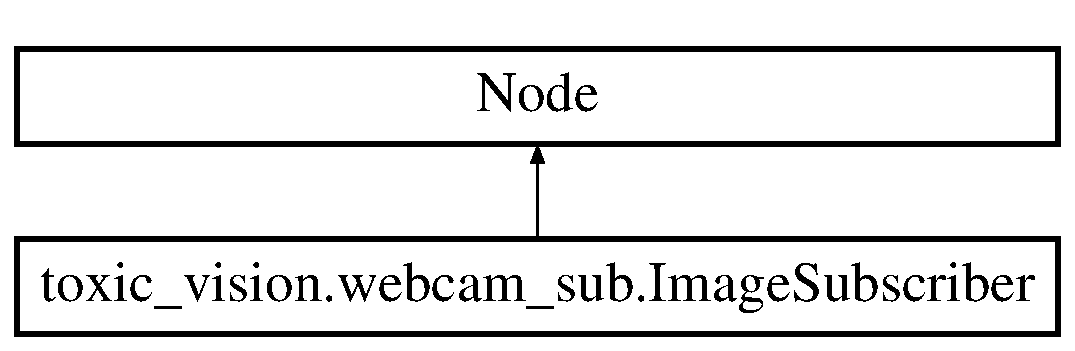
\includegraphics[height=2.000000cm]{db/dd5/classtoxic__vision_1_1webcam__sub_1_1ImageSubscriber}
\end{center}
\end{figure}
\doxysubsection*{Public Member Functions}
\begin{DoxyCompactItemize}
\item 
def \mbox{\hyperlink{classtoxic__vision_1_1webcam__sub_1_1ImageSubscriber_ae64f0875afe3067b97ba370b354b9213}{\+\_\+\+\_\+init\+\_\+\+\_\+}} (self)
\item 
def \mbox{\hyperlink{classtoxic__vision_1_1webcam__sub_1_1ImageSubscriber_a23dd9943cb7cb7be2a6e7022a85a1684}{listener\+\_\+callback}} (self, data)
\item 
def \mbox{\hyperlink{classtoxic__vision_1_1webcam__sub_1_1ImageSubscriber_ae64f0875afe3067b97ba370b354b9213}{\+\_\+\+\_\+init\+\_\+\+\_\+}} (self)
\begin{DoxyCompactList}\small\item\em \mbox{\hyperlink{classtoxic__vision_1_1webcam__sub_1_1ImageSubscriber}{Image\+Subscriber}} object to grab the currently published frame in a ROS2 Topic (this time, it\textquotesingle{}s \textquotesingle{}/raw\+\_\+rgb\textquotesingle{}, but you can change it) and display in a GUI window. \end{DoxyCompactList}\item 
def \mbox{\hyperlink{classtoxic__vision_1_1webcam__sub_1_1ImageSubscriber_a23dd9943cb7cb7be2a6e7022a85a1684}{listener\+\_\+callback}} (self, data)
\end{DoxyCompactItemize}
\doxysubsection*{Public Attributes}
\begin{DoxyCompactItemize}
\item 
\mbox{\hyperlink{classtoxic__vision_1_1webcam__sub_1_1ImageSubscriber_a4b0698733c4dfaffe8e2b4cd952b6f82}{subscription}}
\item 
\mbox{\hyperlink{classtoxic__vision_1_1webcam__sub_1_1ImageSubscriber_a88f0860257ba6bdc089557444f5cdd16}{br}}
\end{DoxyCompactItemize}


\doxysubsection{Constructor \& Destructor Documentation}
\mbox{\Hypertarget{classtoxic__vision_1_1webcam__sub_1_1ImageSubscriber_ae64f0875afe3067b97ba370b354b9213}\label{classtoxic__vision_1_1webcam__sub_1_1ImageSubscriber_ae64f0875afe3067b97ba370b354b9213}} 
\index{ImageSubscriber@{ImageSubscriber}!\_\_init\_\_@{\_\_init\_\_}}
\index{\_\_init\_\_@{\_\_init\_\_}!ImageSubscriber@{ImageSubscriber}}
\doxysubsubsection{\texorpdfstring{\_\_init\_\_()}{\_\_init\_\_()}\hspace{0.1cm}{\footnotesize\ttfamily [1/2]}}
{\footnotesize\ttfamily def \+\_\+\+\_\+init\+\_\+\+\_\+ (\begin{DoxyParamCaption}\item[{}]{self }\end{DoxyParamCaption})}


\begin{DoxyCode}{0}
\DoxyCodeLine{8   \textcolor{keyword}{def }\_\_init\_\_(self):}
\DoxyCodeLine{9     super().\_\_init\_\_(\textcolor{stringliteral}{'image\_subscriber'})}
\DoxyCodeLine{10     self.subscription = self.create\_subscription(}
\DoxyCodeLine{11       Image, }
\DoxyCodeLine{12       \textcolor{stringliteral}{'/raw\_rgb'}, }
\DoxyCodeLine{13       self.listener\_callback, }
\DoxyCodeLine{14       25}
\DoxyCodeLine{15       )}
\DoxyCodeLine{16     self.subscription}
\DoxyCodeLine{17     self.br = CvBridge()}
\DoxyCodeLine{18    }

\end{DoxyCode}
\mbox{\Hypertarget{classtoxic__vision_1_1webcam__sub_1_1ImageSubscriber_ae64f0875afe3067b97ba370b354b9213}\label{classtoxic__vision_1_1webcam__sub_1_1ImageSubscriber_ae64f0875afe3067b97ba370b354b9213}} 
\index{ImageSubscriber@{ImageSubscriber}!\_\_init\_\_@{\_\_init\_\_}}
\index{\_\_init\_\_@{\_\_init\_\_}!ImageSubscriber@{ImageSubscriber}}
\doxysubsubsection{\texorpdfstring{\_\_init\_\_()}{\_\_init\_\_()}\hspace{0.1cm}{\footnotesize\ttfamily [2/2]}}
{\footnotesize\ttfamily def \+\_\+\+\_\+init\+\_\+\+\_\+ (\begin{DoxyParamCaption}\item[{}]{self }\end{DoxyParamCaption})}



\mbox{\hyperlink{classtoxic__vision_1_1webcam__sub_1_1ImageSubscriber}{Image\+Subscriber}} object to grab the currently published frame in a ROS2 Topic (this time, it\textquotesingle{}s \textquotesingle{}/raw\+\_\+rgb\textquotesingle{}, but you can change it) and display in a GUI window. 


\begin{DoxyParams}{Parameters}
{\em Node} & The ROS2 Node where the image publisher\textquotesingle{}ll be able to read/write (this time, just read)\\
\hline
\end{DoxyParams}
\begin{DoxyReturn}{Returns}
None, keeps running and alive until it\textquotesingle{}s user cancelled.
\end{DoxyReturn}
\mbox{\hyperlink{classtoxic__vision_1_1webcam__sub_1_1ImageSubscriber}{Image\+Subscriber}} obtect init def (or constructor, under a Java´s OOP context)


\begin{DoxyParams}{Parameters}
{\em self,Self} & contained object, like a \textquotesingle{}this\textquotesingle{} reference just to read, write and genereally access object\textquotesingle{}s attributes. \\
\hline
\end{DoxyParams}

\begin{DoxyCode}{0}
\DoxyCodeLine{60     \textcolor{keyword}{def }\_\_init\_\_(self):}
\DoxyCodeLine{61         }
\DoxyCodeLine{68         }
\DoxyCodeLine{69         \textcolor{comment}{\# Edit source Node attributes}}
\DoxyCodeLine{70         super().\_\_init\_\_(\textcolor{stringliteral}{'image\_subscriber'})}
\DoxyCodeLine{71         self.subscription = self.create\_subscription(}
\DoxyCodeLine{72                 Image, }
\DoxyCodeLine{73                 \textcolor{stringliteral}{'/raw\_rgb'}, }
\DoxyCodeLine{74                 self.listener\_callback, }
\DoxyCodeLine{75                 25}
\DoxyCodeLine{76                 )}
\DoxyCodeLine{77         self.subscription}
\DoxyCodeLine{78         self.br = CvBridge()}
\DoxyCodeLine{79     }

\end{DoxyCode}


\doxysubsection{Member Function Documentation}
\mbox{\Hypertarget{classtoxic__vision_1_1webcam__sub_1_1ImageSubscriber_a23dd9943cb7cb7be2a6e7022a85a1684}\label{classtoxic__vision_1_1webcam__sub_1_1ImageSubscriber_a23dd9943cb7cb7be2a6e7022a85a1684}} 
\index{ImageSubscriber@{ImageSubscriber}!listener\_callback@{listener\_callback}}
\index{listener\_callback@{listener\_callback}!ImageSubscriber@{ImageSubscriber}}
\doxysubsubsection{\texorpdfstring{listener\_callback()}{listener\_callback()}\hspace{0.1cm}{\footnotesize\ttfamily [1/2]}}
{\footnotesize\ttfamily def listener\+\_\+callback (\begin{DoxyParamCaption}\item[{}]{self,  }\item[{}]{data }\end{DoxyParamCaption})}


\begin{DoxyCode}{0}
\DoxyCodeLine{19   \textcolor{keyword}{def }listener\_callback(self, data):}
\DoxyCodeLine{20     current\_frame = self.br.imgmsg\_to\_cv2(data)}
\DoxyCodeLine{21     cv2.imshow(\textcolor{stringliteral}{"{}band\_filter\_sub"{}}, current\_frame)}
\DoxyCodeLine{22     cv2.waitKey(1)}

\end{DoxyCode}
\mbox{\Hypertarget{classtoxic__vision_1_1webcam__sub_1_1ImageSubscriber_a23dd9943cb7cb7be2a6e7022a85a1684}\label{classtoxic__vision_1_1webcam__sub_1_1ImageSubscriber_a23dd9943cb7cb7be2a6e7022a85a1684}} 
\index{ImageSubscriber@{ImageSubscriber}!listener\_callback@{listener\_callback}}
\index{listener\_callback@{listener\_callback}!ImageSubscriber@{ImageSubscriber}}
\doxysubsubsection{\texorpdfstring{listener\_callback()}{listener\_callback()}\hspace{0.1cm}{\footnotesize\ttfamily [2/2]}}
{\footnotesize\ttfamily def listener\+\_\+callback (\begin{DoxyParamCaption}\item[{}]{self,  }\item[{}]{data }\end{DoxyParamCaption})}


\begin{DoxyCode}{0}
\DoxyCodeLine{80     \textcolor{keyword}{def }listener\_callback(self, data):}
\DoxyCodeLine{81         current\_frame = self.br.imgmsg\_to\_cv2(data)}
\DoxyCodeLine{82         cv2.imshow(\textcolor{stringliteral}{"{}band\_filter\_sub"{}}, current\_frame)}
\DoxyCodeLine{83         cv2.waitKey(1)}

\end{DoxyCode}


\doxysubsection{Member Data Documentation}
\mbox{\Hypertarget{classtoxic__vision_1_1webcam__sub_1_1ImageSubscriber_a88f0860257ba6bdc089557444f5cdd16}\label{classtoxic__vision_1_1webcam__sub_1_1ImageSubscriber_a88f0860257ba6bdc089557444f5cdd16}} 
\index{ImageSubscriber@{ImageSubscriber}!br@{br}}
\index{br@{br}!ImageSubscriber@{ImageSubscriber}}
\doxysubsubsection{\texorpdfstring{br}{br}}
{\footnotesize\ttfamily br}

\mbox{\Hypertarget{classtoxic__vision_1_1webcam__sub_1_1ImageSubscriber_a4b0698733c4dfaffe8e2b4cd952b6f82}\label{classtoxic__vision_1_1webcam__sub_1_1ImageSubscriber_a4b0698733c4dfaffe8e2b4cd952b6f82}} 
\index{ImageSubscriber@{ImageSubscriber}!subscription@{subscription}}
\index{subscription@{subscription}!ImageSubscriber@{ImageSubscriber}}
\doxysubsubsection{\texorpdfstring{subscription}{subscription}}
{\footnotesize\ttfamily subscription}



The documentation for this class was generated from the following file\+:\begin{DoxyCompactItemize}
\item 
main\+\_\+ws/build/toxic\+\_\+vision/build/lib/toxic\+\_\+vision/\mbox{\hyperlink{build_2toxic__vision_2build_2lib_2toxic__vision_2webcam__sub_8py}{webcam\+\_\+sub.\+py}}\end{DoxyCompactItemize}

\hypertarget{classtoxic__hardware_1_1motor__interface_1_1MotorInterface}{}\section{toxic\+\_\+hardware.\+motor\+\_\+interface.\+Motor\+Interface Class Reference}
\label{classtoxic__hardware_1_1motor__interface_1_1MotorInterface}\index{toxic\+\_\+hardware.\+motor\+\_\+interface.\+Motor\+Interface@{toxic\+\_\+hardware.\+motor\+\_\+interface.\+Motor\+Interface}}
Inheritance diagram for toxic\+\_\+hardware.\+motor\+\_\+interface.\+Motor\+Interface\+:\begin{figure}[H]
\begin{center}
\leavevmode
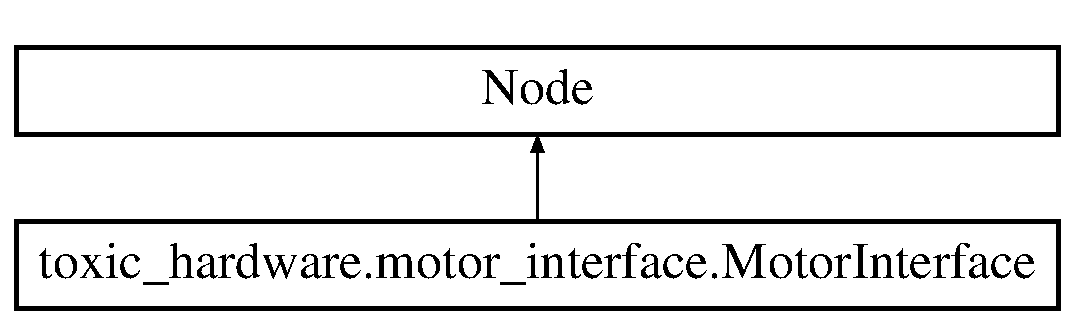
\includegraphics[height=2.000000cm]{d6/dfb/classtoxic__hardware_1_1motor__interface_1_1MotorInterface}
\end{center}
\end{figure}
\subsection*{Public Member Functions}
\begin{DoxyCompactItemize}
\item 
def \mbox{\hyperlink{classtoxic__hardware_1_1motor__interface_1_1MotorInterface_a8264a67be5aa9dbecbe12d06bd1b6b29}{\+\_\+\+\_\+init\+\_\+\+\_\+}} (self)
\item 
def \mbox{\hyperlink{classtoxic__hardware_1_1motor__interface_1_1MotorInterface_a03f00bab38c0702cf53e679ef2ae8216}{motor\+\_\+callback}} (self, data)
\end{DoxyCompactItemize}
\subsection*{Public Attributes}
\begin{DoxyCompactItemize}
\item 
\mbox{\hyperlink{classtoxic__hardware_1_1motor__interface_1_1MotorInterface_afb6296197761247831d86469a6b783dc}{subscription}}
\end{DoxyCompactItemize}


\subsection{Constructor \& Destructor Documentation}
\mbox{\Hypertarget{classtoxic__hardware_1_1motor__interface_1_1MotorInterface_a8264a67be5aa9dbecbe12d06bd1b6b29}\label{classtoxic__hardware_1_1motor__interface_1_1MotorInterface_a8264a67be5aa9dbecbe12d06bd1b6b29}} 
\index{toxic\+\_\+hardware\+::motor\+\_\+interface\+::\+Motor\+Interface@{toxic\+\_\+hardware\+::motor\+\_\+interface\+::\+Motor\+Interface}!\+\_\+\+\_\+init\+\_\+\+\_\+@{\+\_\+\+\_\+init\+\_\+\+\_\+}}
\index{\+\_\+\+\_\+init\+\_\+\+\_\+@{\+\_\+\+\_\+init\+\_\+\+\_\+}!toxic\+\_\+hardware\+::motor\+\_\+interface\+::\+Motor\+Interface@{toxic\+\_\+hardware\+::motor\+\_\+interface\+::\+Motor\+Interface}}
\subsubsection{\texorpdfstring{\+\_\+\+\_\+init\+\_\+\+\_\+()}{\_\_init\_\_()}}
{\footnotesize\ttfamily def toxic\+\_\+hardware.\+motor\+\_\+interface.\+Motor\+Interface.\+\_\+\+\_\+init\+\_\+\+\_\+ (\begin{DoxyParamCaption}\item[{}]{self }\end{DoxyParamCaption})}



\subsection{Member Function Documentation}
\mbox{\Hypertarget{classtoxic__hardware_1_1motor__interface_1_1MotorInterface_a03f00bab38c0702cf53e679ef2ae8216}\label{classtoxic__hardware_1_1motor__interface_1_1MotorInterface_a03f00bab38c0702cf53e679ef2ae8216}} 
\index{toxic\+\_\+hardware\+::motor\+\_\+interface\+::\+Motor\+Interface@{toxic\+\_\+hardware\+::motor\+\_\+interface\+::\+Motor\+Interface}!motor\+\_\+callback@{motor\+\_\+callback}}
\index{motor\+\_\+callback@{motor\+\_\+callback}!toxic\+\_\+hardware\+::motor\+\_\+interface\+::\+Motor\+Interface@{toxic\+\_\+hardware\+::motor\+\_\+interface\+::\+Motor\+Interface}}
\subsubsection{\texorpdfstring{motor\+\_\+callback()}{motor\_callback()}}
{\footnotesize\ttfamily def toxic\+\_\+hardware.\+motor\+\_\+interface.\+Motor\+Interface.\+motor\+\_\+callback (\begin{DoxyParamCaption}\item[{}]{self,  }\item[{}]{data }\end{DoxyParamCaption})}



\subsection{Member Data Documentation}
\mbox{\Hypertarget{classtoxic__hardware_1_1motor__interface_1_1MotorInterface_afb6296197761247831d86469a6b783dc}\label{classtoxic__hardware_1_1motor__interface_1_1MotorInterface_afb6296197761247831d86469a6b783dc}} 
\index{toxic\+\_\+hardware\+::motor\+\_\+interface\+::\+Motor\+Interface@{toxic\+\_\+hardware\+::motor\+\_\+interface\+::\+Motor\+Interface}!subscription@{subscription}}
\index{subscription@{subscription}!toxic\+\_\+hardware\+::motor\+\_\+interface\+::\+Motor\+Interface@{toxic\+\_\+hardware\+::motor\+\_\+interface\+::\+Motor\+Interface}}
\subsubsection{\texorpdfstring{subscription}{subscription}}
{\footnotesize\ttfamily toxic\+\_\+hardware.\+motor\+\_\+interface.\+Motor\+Interface.\+subscription}



The documentation for this class was generated from the following file\+:\begin{DoxyCompactItemize}
\item 
main\+\_\+ws/src/toxic\+\_\+hardware/toxic\+\_\+hardware/\mbox{\hyperlink{motor__interface_8py}{motor\+\_\+interface.\+py}}\end{DoxyCompactItemize}

\hypertarget{classtoxic__hardware_1_1oled__interface_1_1OledInterface}{}\doxysection{Oled\+Interface Class Reference}
\label{classtoxic__hardware_1_1oled__interface_1_1OledInterface}\index{OledInterface@{OledInterface}}
Inheritance diagram for Oled\+Interface\+:\begin{figure}[H]
\begin{center}
\leavevmode
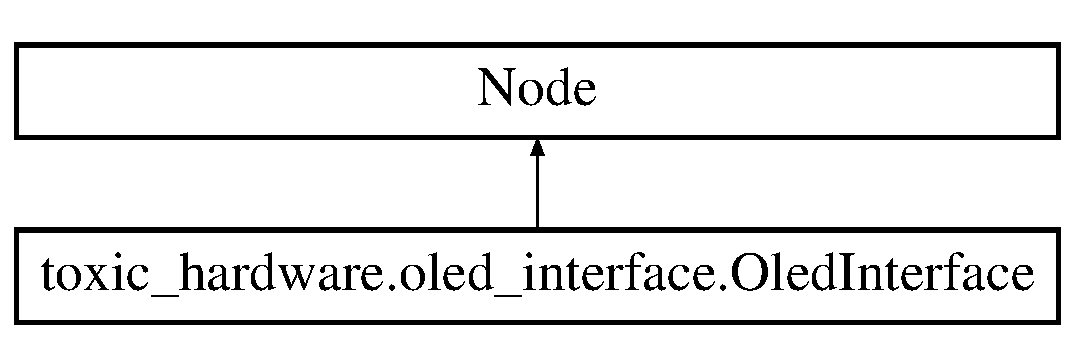
\includegraphics[height=2.000000cm]{d9/d4e/classtoxic__hardware_1_1oled__interface_1_1OledInterface}
\end{center}
\end{figure}
\doxysubsection*{Public Member Functions}
\begin{DoxyCompactItemize}
\item 
def \mbox{\hyperlink{classtoxic__hardware_1_1oled__interface_1_1OledInterface_ae64f0875afe3067b97ba370b354b9213}{\+\_\+\+\_\+init\+\_\+\+\_\+}} (self)
\item 
def \mbox{\hyperlink{classtoxic__hardware_1_1oled__interface_1_1OledInterface_a956e7ab59d12fa1dc3e975c2fba46296}{oled\+\_\+callback}} (self, data)
\item 
def \mbox{\hyperlink{classtoxic__hardware_1_1oled__interface_1_1OledInterface_ae64f0875afe3067b97ba370b354b9213}{\+\_\+\+\_\+init\+\_\+\+\_\+}} (self)
\item 
def \mbox{\hyperlink{classtoxic__hardware_1_1oled__interface_1_1OledInterface_a956e7ab59d12fa1dc3e975c2fba46296}{oled\+\_\+callback}} (self, data)
\end{DoxyCompactItemize}
\doxysubsection*{Public Attributes}
\begin{DoxyCompactItemize}
\item 
\mbox{\hyperlink{classtoxic__hardware_1_1oled__interface_1_1OledInterface_a4b0698733c4dfaffe8e2b4cd952b6f82}{subscription}}
\end{DoxyCompactItemize}


\doxysubsection{Constructor \& Destructor Documentation}
\mbox{\Hypertarget{classtoxic__hardware_1_1oled__interface_1_1OledInterface_ae64f0875afe3067b97ba370b354b9213}\label{classtoxic__hardware_1_1oled__interface_1_1OledInterface_ae64f0875afe3067b97ba370b354b9213}} 
\index{OledInterface@{OledInterface}!\_\_init\_\_@{\_\_init\_\_}}
\index{\_\_init\_\_@{\_\_init\_\_}!OledInterface@{OledInterface}}
\doxysubsubsection{\texorpdfstring{\_\_init\_\_()}{\_\_init\_\_()}\hspace{0.1cm}{\footnotesize\ttfamily [1/2]}}
{\footnotesize\ttfamily def \+\_\+\+\_\+init\+\_\+\+\_\+ (\begin{DoxyParamCaption}\item[{}]{self }\end{DoxyParamCaption})}


\begin{DoxyCode}{0}
\DoxyCodeLine{39     \textcolor{keyword}{def }\_\_init\_\_(self):}
\DoxyCodeLine{40         super().\_\_init\_\_(\textcolor{stringliteral}{'oled\_interface'})}
\DoxyCodeLine{41         self.subscription = self.create\_subscription(}
\DoxyCodeLine{42                 String,}
\DoxyCodeLine{43                 \textcolor{stringliteral}{'/message'},}
\DoxyCodeLine{44                 self.oled\_callback,}
\DoxyCodeLine{45                 60}
\DoxyCodeLine{46         )}
\DoxyCodeLine{47 }

\end{DoxyCode}
\mbox{\Hypertarget{classtoxic__hardware_1_1oled__interface_1_1OledInterface_ae64f0875afe3067b97ba370b354b9213}\label{classtoxic__hardware_1_1oled__interface_1_1OledInterface_ae64f0875afe3067b97ba370b354b9213}} 
\index{OledInterface@{OledInterface}!\_\_init\_\_@{\_\_init\_\_}}
\index{\_\_init\_\_@{\_\_init\_\_}!OledInterface@{OledInterface}}
\doxysubsubsection{\texorpdfstring{\_\_init\_\_()}{\_\_init\_\_()}\hspace{0.1cm}{\footnotesize\ttfamily [2/2]}}
{\footnotesize\ttfamily def \+\_\+\+\_\+init\+\_\+\+\_\+ (\begin{DoxyParamCaption}\item[{}]{self }\end{DoxyParamCaption})}


\begin{DoxyCode}{0}
\DoxyCodeLine{39     \textcolor{keyword}{def }\_\_init\_\_(self):}
\DoxyCodeLine{40         super().\_\_init\_\_(\textcolor{stringliteral}{'oled\_interface'})}
\DoxyCodeLine{41         self.subscription = self.create\_subscription(}
\DoxyCodeLine{42                 String,}
\DoxyCodeLine{43                 \textcolor{stringliteral}{'/message'},}
\DoxyCodeLine{44                 self.oled\_callback,}
\DoxyCodeLine{45                 60}
\DoxyCodeLine{46         )}
\DoxyCodeLine{47 }

\end{DoxyCode}


\doxysubsection{Member Function Documentation}
\mbox{\Hypertarget{classtoxic__hardware_1_1oled__interface_1_1OledInterface_a956e7ab59d12fa1dc3e975c2fba46296}\label{classtoxic__hardware_1_1oled__interface_1_1OledInterface_a956e7ab59d12fa1dc3e975c2fba46296}} 
\index{OledInterface@{OledInterface}!oled\_callback@{oled\_callback}}
\index{oled\_callback@{oled\_callback}!OledInterface@{OledInterface}}
\doxysubsubsection{\texorpdfstring{oled\_callback()}{oled\_callback()}\hspace{0.1cm}{\footnotesize\ttfamily [1/2]}}
{\footnotesize\ttfamily def oled\+\_\+callback (\begin{DoxyParamCaption}\item[{}]{self,  }\item[{}]{data }\end{DoxyParamCaption})}


\begin{DoxyCode}{0}
\DoxyCodeLine{48     \textcolor{keyword}{def }oled\_callback(self, data):}
\DoxyCodeLine{49         \textcolor{keyword}{global} draw, image}
\DoxyCodeLine{50         draw.rectangle((0,0,width,height), outline=0, fill=0)}
\DoxyCodeLine{51         msg\_content = data.data}
\DoxyCodeLine{52         draw.text((x, top), msg\_content,  font=font, fill=255)}
\DoxyCodeLine{53         disp.image(image)}
\DoxyCodeLine{54         disp.display()}
\DoxyCodeLine{55 }

\end{DoxyCode}
\mbox{\Hypertarget{classtoxic__hardware_1_1oled__interface_1_1OledInterface_a956e7ab59d12fa1dc3e975c2fba46296}\label{classtoxic__hardware_1_1oled__interface_1_1OledInterface_a956e7ab59d12fa1dc3e975c2fba46296}} 
\index{OledInterface@{OledInterface}!oled\_callback@{oled\_callback}}
\index{oled\_callback@{oled\_callback}!OledInterface@{OledInterface}}
\doxysubsubsection{\texorpdfstring{oled\_callback()}{oled\_callback()}\hspace{0.1cm}{\footnotesize\ttfamily [2/2]}}
{\footnotesize\ttfamily def oled\+\_\+callback (\begin{DoxyParamCaption}\item[{}]{self,  }\item[{}]{data }\end{DoxyParamCaption})}


\begin{DoxyCode}{0}
\DoxyCodeLine{48     \textcolor{keyword}{def }oled\_callback(self, data):}
\DoxyCodeLine{49         \textcolor{keyword}{global} draw, image}
\DoxyCodeLine{50         draw.rectangle((0,0,width,height), outline=0, fill=0)}
\DoxyCodeLine{51         msg\_content = data.data}
\DoxyCodeLine{52         draw.text((x, top), msg\_content,  font=font, fill=255)}
\DoxyCodeLine{53         disp.image(image)}
\DoxyCodeLine{54         disp.display()}
\DoxyCodeLine{55 }

\end{DoxyCode}


\doxysubsection{Member Data Documentation}
\mbox{\Hypertarget{classtoxic__hardware_1_1oled__interface_1_1OledInterface_a4b0698733c4dfaffe8e2b4cd952b6f82}\label{classtoxic__hardware_1_1oled__interface_1_1OledInterface_a4b0698733c4dfaffe8e2b4cd952b6f82}} 
\index{OledInterface@{OledInterface}!subscription@{subscription}}
\index{subscription@{subscription}!OledInterface@{OledInterface}}
\doxysubsubsection{\texorpdfstring{subscription}{subscription}}
{\footnotesize\ttfamily subscription}



The documentation for this class was generated from the following file\+:\begin{DoxyCompactItemize}
\item 
main\+\_\+ws/build/toxic\+\_\+hardware/build/lib/toxic\+\_\+hardware/\mbox{\hyperlink{build_2toxic__hardware_2build_2lib_2toxic__hardware_2oled__interface_8py}{oled\+\_\+interface.\+py}}\end{DoxyCompactItemize}

\hypertarget{classtoxic__hardware_1_1roboclaw__3_1_1Roboclaw}{}\section{Roboclaw Class Reference}
\label{classtoxic__hardware_1_1roboclaw__3_1_1Roboclaw}\index{Roboclaw@{Roboclaw}}
\subsection*{Classes}
\begin{DoxyCompactItemize}
\item 
class \mbox{\hyperlink{classtoxic__hardware_1_1roboclaw__3_1_1Roboclaw_1_1Cmd}{Cmd}}
\end{DoxyCompactItemize}
\subsection*{Public Member Functions}
\begin{DoxyCompactItemize}
\item 
def \mbox{\hyperlink{classtoxic__hardware_1_1roboclaw__3_1_1Roboclaw_a0f9f3612daa4ca7ffa720a9d3b4b3417}{\+\_\+\+\_\+init\+\_\+\+\_\+}} (self, \mbox{\hyperlink{classtoxic__hardware_1_1roboclaw__3_1_1Roboclaw_af11cdc24a14ee681791b216a58a596a9}{comport}}, \mbox{\hyperlink{classtoxic__hardware_1_1roboclaw__3_1_1Roboclaw_a1d580470818c2fa51a0bf3a86bc595bf}{rate}}, \mbox{\hyperlink{classtoxic__hardware_1_1roboclaw__3_1_1Roboclaw_aee145bfca8e9b2eaf3cd3c47157be9a3}{timeout}}=0.\+01, retries=3)
\item 
def \mbox{\hyperlink{classtoxic__hardware_1_1roboclaw__3_1_1Roboclaw_a13d25f23765d6d691a12540125b17108}{crc\+\_\+clear}} (self)
\item 
def \mbox{\hyperlink{classtoxic__hardware_1_1roboclaw__3_1_1Roboclaw_ab0194da7d3b1e01752a7d24dee8c7b55}{crc\+\_\+update}} (self, data)
\item 
def \mbox{\hyperlink{classtoxic__hardware_1_1roboclaw__3_1_1Roboclaw_ae99acedd53fe667ff7bed5d38a6859bd}{Send\+Random\+Data}} (self, cnt)
\item 
def \mbox{\hyperlink{classtoxic__hardware_1_1roboclaw__3_1_1Roboclaw_adf9ab5d77d53912be9929f7ed8e6e05f}{Forward\+M1}} (self, address, val)
\item 
def \mbox{\hyperlink{classtoxic__hardware_1_1roboclaw__3_1_1Roboclaw_a33caa5eb9a19e9d3dc648bd1e49cf5ea}{Backward\+M1}} (self, address, val)
\item 
def \mbox{\hyperlink{classtoxic__hardware_1_1roboclaw__3_1_1Roboclaw_a7e011acf85a7b17384719def6997dde8}{Set\+Min\+Voltage\+Main\+Battery}} (self, address, val)
\item 
def \mbox{\hyperlink{classtoxic__hardware_1_1roboclaw__3_1_1Roboclaw_ad2c3c89aa38f0d616778f71128a6ca08}{Set\+Max\+Voltage\+Main\+Battery}} (self, address, val)
\item 
def \mbox{\hyperlink{classtoxic__hardware_1_1roboclaw__3_1_1Roboclaw_abce41d003f6c4583a79616837749db3f}{Forward\+M2}} (self, address, val)
\item 
def \mbox{\hyperlink{classtoxic__hardware_1_1roboclaw__3_1_1Roboclaw_a291d3a943191a562dd0c726430a45c9c}{Backward\+M2}} (self, address, val)
\item 
def \mbox{\hyperlink{classtoxic__hardware_1_1roboclaw__3_1_1Roboclaw_aa2371adb932a68762fe3996c2be8a3ba}{Forward\+Backward\+M1}} (self, address, val)
\item 
def \mbox{\hyperlink{classtoxic__hardware_1_1roboclaw__3_1_1Roboclaw_a72bcc49b759cda4a3de15a6292a28296}{Forward\+Backward\+M2}} (self, address, val)
\item 
def \mbox{\hyperlink{classtoxic__hardware_1_1roboclaw__3_1_1Roboclaw_acf82a90e2bcb68c83166a1be4978a556}{Forward\+Mixed}} (self, address, val)
\item 
def \mbox{\hyperlink{classtoxic__hardware_1_1roboclaw__3_1_1Roboclaw_a72ca8ef69781031cffede46595df8426}{Backward\+Mixed}} (self, address, val)
\item 
def \mbox{\hyperlink{classtoxic__hardware_1_1roboclaw__3_1_1Roboclaw_ad05d76efd4822a8f8ee8a558820083c8}{Turn\+Right\+Mixed}} (self, address, val)
\item 
def \mbox{\hyperlink{classtoxic__hardware_1_1roboclaw__3_1_1Roboclaw_aafa3ee25f590d5f4b0259f38b32bd626}{Turn\+Left\+Mixed}} (self, address, val)
\item 
def \mbox{\hyperlink{classtoxic__hardware_1_1roboclaw__3_1_1Roboclaw_a1895e1f56aaf7909852db2e576f59d2d}{Forward\+Backward\+Mixed}} (self, address, val)
\item 
def \mbox{\hyperlink{classtoxic__hardware_1_1roboclaw__3_1_1Roboclaw_ab1b403df0c19b03fa19fc6e6944b5bac}{Left\+Right\+Mixed}} (self, address, val)
\item 
def \mbox{\hyperlink{classtoxic__hardware_1_1roboclaw__3_1_1Roboclaw_a912ba280064ac04e9d69e7333da9c143}{Read\+Enc\+M1}} (self, address)
\item 
def \mbox{\hyperlink{classtoxic__hardware_1_1roboclaw__3_1_1Roboclaw_a070a811f611cd1b8c86c375eac24cd71}{Read\+Enc\+M2}} (self, address)
\item 
def \mbox{\hyperlink{classtoxic__hardware_1_1roboclaw__3_1_1Roboclaw_a4f1e923998c2561bbb86a04bc32df602}{Read\+Speed\+M1}} (self, address)
\item 
def \mbox{\hyperlink{classtoxic__hardware_1_1roboclaw__3_1_1Roboclaw_a9336d97afea54d955d7d241ac930bd18}{Read\+Speed\+M2}} (self, address)
\item 
def \mbox{\hyperlink{classtoxic__hardware_1_1roboclaw__3_1_1Roboclaw_ad6017e671abf27badfd65aa559a80681}{Reset\+Encoders}} (self, address)
\item 
def \mbox{\hyperlink{classtoxic__hardware_1_1roboclaw__3_1_1Roboclaw_ab0622e3f1cf0d537b1b4b73bde02fbe1}{Read\+Version}} (self, address)
\item 
def \mbox{\hyperlink{classtoxic__hardware_1_1roboclaw__3_1_1Roboclaw_a534607e041ee0ebe7cc66261071b537d}{Set\+Enc\+M1}} (self, address, cnt)
\item 
def \mbox{\hyperlink{classtoxic__hardware_1_1roboclaw__3_1_1Roboclaw_a8b54c048cc6b6aa19d4123f3d78dfb54}{Set\+Enc\+M2}} (self, address, cnt)
\item 
def \mbox{\hyperlink{classtoxic__hardware_1_1roboclaw__3_1_1Roboclaw_abb5901cba752131303b0378bbaf59c38}{Read\+Main\+Battery\+Voltage}} (self, address)
\item 
def \mbox{\hyperlink{classtoxic__hardware_1_1roboclaw__3_1_1Roboclaw_aac164c773247f222999594aba2deae95}{Read\+Logic\+Battery\+Voltage}} (self, address)
\item 
def \mbox{\hyperlink{classtoxic__hardware_1_1roboclaw__3_1_1Roboclaw_adb683d1e84a0432cca192f662407904f}{Set\+Min\+Voltage\+Logic\+Battery}} (self, address, val)
\item 
def \mbox{\hyperlink{classtoxic__hardware_1_1roboclaw__3_1_1Roboclaw_a726fe4e542430464c2fc2bf14f5142a3}{Set\+Max\+Voltage\+Logic\+Battery}} (self, address, val)
\item 
def \mbox{\hyperlink{classtoxic__hardware_1_1roboclaw__3_1_1Roboclaw_a8ea4c0748b43e086bf7326ec1cd1d8f5}{Set\+M1\+Velocity\+P\+ID}} (self, address, p, i, d, qpps)
\item 
def \mbox{\hyperlink{classtoxic__hardware_1_1roboclaw__3_1_1Roboclaw_aea08bdecff46652920d96fc6239ae604}{Set\+M2\+Velocity\+P\+ID}} (self, address, p, i, d, qpps)
\item 
def \mbox{\hyperlink{classtoxic__hardware_1_1roboclaw__3_1_1Roboclaw_a26242513f458febf217714b304956f11}{Read\+I\+Speed\+M1}} (self, address)
\item 
def \mbox{\hyperlink{classtoxic__hardware_1_1roboclaw__3_1_1Roboclaw_aaac3abe9920b64707f1697b870bd16fd}{Read\+I\+Speed\+M2}} (self, address)
\item 
def \mbox{\hyperlink{classtoxic__hardware_1_1roboclaw__3_1_1Roboclaw_afd7c4865f7e4c723f66b5b51ce8069d3}{Duty\+M1}} (self, address, val)
\item 
def \mbox{\hyperlink{classtoxic__hardware_1_1roboclaw__3_1_1Roboclaw_a99a7bb8b0e944f465bbeb1b6722ef22c}{Duty\+M2}} (self, address, val)
\item 
def \mbox{\hyperlink{classtoxic__hardware_1_1roboclaw__3_1_1Roboclaw_a3f7c1baa59d28bf69d9beb6a83deab5f}{Duty\+M1\+M2}} (self, address, m1, m2)
\item 
def \mbox{\hyperlink{classtoxic__hardware_1_1roboclaw__3_1_1Roboclaw_af4f6babccd668312895a4a4b04a262d4}{Speed\+M1}} (self, address, val)
\item 
def \mbox{\hyperlink{classtoxic__hardware_1_1roboclaw__3_1_1Roboclaw_afa7cb556973974794bc2d040eabde676}{Speed\+M2}} (self, address, val)
\item 
def \mbox{\hyperlink{classtoxic__hardware_1_1roboclaw__3_1_1Roboclaw_ae8f0e90249e078ce5de6930dbabb338d}{Speed\+M1\+M2}} (self, address, m1, m2)
\item 
def \mbox{\hyperlink{classtoxic__hardware_1_1roboclaw__3_1_1Roboclaw_aed66489886b7cfdaaeb2be6cda59427c}{Speed\+Accel\+M1}} (self, address, accel, speed)
\item 
def \mbox{\hyperlink{classtoxic__hardware_1_1roboclaw__3_1_1Roboclaw_ac9b5288bf09d899fb2891fa4a1cb5326}{Speed\+Accel\+M2}} (self, address, accel, speed)
\item 
def \mbox{\hyperlink{classtoxic__hardware_1_1roboclaw__3_1_1Roboclaw_a5e5e1072e698207b50ecf2f6adf5e367}{Speed\+Accel\+M1\+M2}} (self, address, accel, speed1, speed2)
\item 
def \mbox{\hyperlink{classtoxic__hardware_1_1roboclaw__3_1_1Roboclaw_a6664490ee5bec1b0c496b148c9b3f4c7}{Speed\+Distance\+M1}} (self, address, speed, distance, buffer)
\item 
def \mbox{\hyperlink{classtoxic__hardware_1_1roboclaw__3_1_1Roboclaw_a6469781a5630e53aa70f19cf603cfcc0}{Speed\+Distance\+M2}} (self, address, speed, distance, buffer)
\item 
def \mbox{\hyperlink{classtoxic__hardware_1_1roboclaw__3_1_1Roboclaw_ac0664ea79d863b5f153a7a3dac18222d}{Speed\+Distance\+M1\+M2}} (self, address, speed1, distance1, speed2, distance2, buffer)
\item 
def \mbox{\hyperlink{classtoxic__hardware_1_1roboclaw__3_1_1Roboclaw_a111c7779f07f5757ba9ba7e93b0edb39}{Speed\+Accel\+Distance\+M1}} (self, address, accel, speed, distance, buffer)
\item 
def \mbox{\hyperlink{classtoxic__hardware_1_1roboclaw__3_1_1Roboclaw_a445110f8fd4f9bbf61bcd9c4a5144ad7}{Speed\+Accel\+Distance\+M2}} (self, address, accel, speed, distance, buffer)
\item 
def \mbox{\hyperlink{classtoxic__hardware_1_1roboclaw__3_1_1Roboclaw_ac2b210f5288d22c653c019bd60ee7fda}{Speed\+Accel\+Distance\+M1\+M2}} (self, address, accel, speed1, distance1, speed2, distance2, buffer)
\item 
def \mbox{\hyperlink{classtoxic__hardware_1_1roboclaw__3_1_1Roboclaw_a0ccc774bd702e611c98c01313707b8fe}{Read\+Buffers}} (self, address)
\item 
def \mbox{\hyperlink{classtoxic__hardware_1_1roboclaw__3_1_1Roboclaw_ad6694602dd7294a517f29dfcbf0a3068}{Read\+P\+W\+Ms}} (self, address)
\item 
def \mbox{\hyperlink{classtoxic__hardware_1_1roboclaw__3_1_1Roboclaw_ac9359f88c9e1b9b23e09ba962bc2774e}{Read\+Currents}} (self, address)
\item 
def \mbox{\hyperlink{classtoxic__hardware_1_1roboclaw__3_1_1Roboclaw_ab9eb6d09f652e887dd9d6b8d1300d919}{Speed\+Accel\+M1\+M2\+\_\+2}} (self, address, accel1, speed1, accel2, speed2)
\item 
def \mbox{\hyperlink{classtoxic__hardware_1_1roboclaw__3_1_1Roboclaw_a2cf733613d498449053cbb0ddc964205}{Speed\+Accel\+Distance\+M1\+M2\+\_\+2}} (self, address, accel1, speed1, distance1, accel2, speed2, distance2, buffer)
\item 
def \mbox{\hyperlink{classtoxic__hardware_1_1roboclaw__3_1_1Roboclaw_a9a743669aa5263257f5443fc24d171fe}{Duty\+Accel\+M1}} (self, address, accel, duty)
\item 
def \mbox{\hyperlink{classtoxic__hardware_1_1roboclaw__3_1_1Roboclaw_a881053800292742cd8419a6158fe36ca}{Duty\+Accel\+M2}} (self, address, accel, duty)
\item 
def \mbox{\hyperlink{classtoxic__hardware_1_1roboclaw__3_1_1Roboclaw_a2aba2edd06d47a93e81ec7f3f3619f59}{Duty\+Accel\+M1\+M2}} (self, address, accel1, duty1, accel2, duty2)
\item 
def \mbox{\hyperlink{classtoxic__hardware_1_1roboclaw__3_1_1Roboclaw_a7d6b9aed2767ac9e9a7df14cde48efe8}{Read\+M1\+Velocity\+P\+ID}} (self, address)
\item 
def \mbox{\hyperlink{classtoxic__hardware_1_1roboclaw__3_1_1Roboclaw_a6130b63fbb5a30686b1f356a3429f0c2}{Read\+M2\+Velocity\+P\+ID}} (self, address)
\item 
def \mbox{\hyperlink{classtoxic__hardware_1_1roboclaw__3_1_1Roboclaw_acd85be507ba58fcd9d3456519c8aff9e}{Set\+Main\+Voltages}} (self, address, min, max)
\item 
def \mbox{\hyperlink{classtoxic__hardware_1_1roboclaw__3_1_1Roboclaw_a9a09e4eb5551bbd1738c4bec30c9519a}{Set\+Logic\+Voltages}} (self, address, min, max)
\item 
def \mbox{\hyperlink{classtoxic__hardware_1_1roboclaw__3_1_1Roboclaw_a5ca4a184f6501b75d547c6bdcbf3735f}{Read\+Min\+Max\+Main\+Voltages}} (self, address)
\item 
def \mbox{\hyperlink{classtoxic__hardware_1_1roboclaw__3_1_1Roboclaw_a6b08f6579fda6d73bc23b5ebe628f952}{Read\+Min\+Max\+Logic\+Voltages}} (self, address)
\item 
def \mbox{\hyperlink{classtoxic__hardware_1_1roboclaw__3_1_1Roboclaw_a86e5bc8af684f784abe72eac70851f3e}{Set\+M1\+Position\+P\+ID}} (self, address, kp, ki, kd, kimax, deadzone, min, max)
\item 
def \mbox{\hyperlink{classtoxic__hardware_1_1roboclaw__3_1_1Roboclaw_af20c35ba0d15081a0fe691601b7457e7}{Set\+M2\+Position\+P\+ID}} (self, address, kp, ki, kd, kimax, deadzone, min, max)
\item 
def \mbox{\hyperlink{classtoxic__hardware_1_1roboclaw__3_1_1Roboclaw_a570e8879933adbcb33e90eb45091fc31}{Read\+M1\+Position\+P\+ID}} (self, address)
\item 
def \mbox{\hyperlink{classtoxic__hardware_1_1roboclaw__3_1_1Roboclaw_a88fdebf9a672c22ff3789719b39dd994}{Read\+M2\+Position\+P\+ID}} (self, address)
\item 
def \mbox{\hyperlink{classtoxic__hardware_1_1roboclaw__3_1_1Roboclaw_a1b4d92f94801f58a9890c9587bd028af}{Speed\+Accel\+Deccel\+Position\+M1}} (self, address, accel, speed, deccel, position, buffer)
\item 
def \mbox{\hyperlink{classtoxic__hardware_1_1roboclaw__3_1_1Roboclaw_ae7008907206f5accff98fe60a85dc124}{Speed\+Accel\+Deccel\+Position\+M2}} (self, address, accel, speed, deccel, position, buffer)
\item 
def \mbox{\hyperlink{classtoxic__hardware_1_1roboclaw__3_1_1Roboclaw_a67d7a0f215dd04abdc264e6f86186542}{Speed\+Accel\+Deccel\+Position\+M1\+M2}} (self, address, accel1, speed1, deccel1, position1, accel2, speed2, deccel2, position2, buffer)
\item 
def \mbox{\hyperlink{classtoxic__hardware_1_1roboclaw__3_1_1Roboclaw_a23dc1a25b115d6e1cecdfacdaef1a723}{Set\+M1\+Default\+Accel}} (self, address, accel)
\item 
def \mbox{\hyperlink{classtoxic__hardware_1_1roboclaw__3_1_1Roboclaw_a039c9127b396a47d39682cf528d66fd4}{Set\+M2\+Default\+Accel}} (self, address, accel)
\item 
def \mbox{\hyperlink{classtoxic__hardware_1_1roboclaw__3_1_1Roboclaw_ac54b2cb80b2ab567fb290a6c376c07a7}{Set\+Pin\+Functions}} (self, address, S3mode, S4mode, S5mode)
\item 
def \mbox{\hyperlink{classtoxic__hardware_1_1roboclaw__3_1_1Roboclaw_a514dcfe31df7d312ed3d2a45666500c3}{Read\+Pin\+Functions}} (self, address)
\item 
def \mbox{\hyperlink{classtoxic__hardware_1_1roboclaw__3_1_1Roboclaw_a5c7b72a7a931b568bb6598b3c9c88dde}{Set\+Dead\+Band}} (self, address, min, max)
\item 
def \mbox{\hyperlink{classtoxic__hardware_1_1roboclaw__3_1_1Roboclaw_afc265149c1e2c828615710da9984db1a}{Get\+Dead\+Band}} (self, address)
\item 
def \mbox{\hyperlink{classtoxic__hardware_1_1roboclaw__3_1_1Roboclaw_ae963de53e2a3be675dc00949c099140a}{Restore\+Defaults}} (self, address)
\item 
def \mbox{\hyperlink{classtoxic__hardware_1_1roboclaw__3_1_1Roboclaw_a4d3216ee6c9260f2ebd116bf6c057d0c}{Read\+Temp}} (self, address)
\item 
def \mbox{\hyperlink{classtoxic__hardware_1_1roboclaw__3_1_1Roboclaw_a2ad329a177d6b02dfd1cd59163c129c5}{Read\+Temp2}} (self, address)
\item 
def \mbox{\hyperlink{classtoxic__hardware_1_1roboclaw__3_1_1Roboclaw_a72e3c01c236d0507a5bbe51dbc4cab7c}{Read\+Error}} (self, address)
\item 
def \mbox{\hyperlink{classtoxic__hardware_1_1roboclaw__3_1_1Roboclaw_a1cef86af310cc021bdf421bd4d02adf3}{Read\+Encoder\+Modes}} (self, address)
\item 
def \mbox{\hyperlink{classtoxic__hardware_1_1roboclaw__3_1_1Roboclaw_ac32404cfafd3dd0c49983b724717945b}{Set\+M1\+Encoder\+Mode}} (self, address, mode)
\item 
def \mbox{\hyperlink{classtoxic__hardware_1_1roboclaw__3_1_1Roboclaw_abc897b52a6653ae79b5c7c193a88345c}{Set\+M2\+Encoder\+Mode}} (self, address, mode)
\item 
def \mbox{\hyperlink{classtoxic__hardware_1_1roboclaw__3_1_1Roboclaw_ab727e2cb1e1d5962f9d52c7af8524ede}{Write\+N\+VM}} (self, address)
\item 
def \mbox{\hyperlink{classtoxic__hardware_1_1roboclaw__3_1_1Roboclaw_a9758a592cc718d5ccc89d45e785d9662}{Read\+N\+VM}} (self, address)
\item 
def \mbox{\hyperlink{classtoxic__hardware_1_1roboclaw__3_1_1Roboclaw_a28cd21a66d7035f83fc68d761c630a85}{Set\+Config}} (self, address, config)
\item 
def \mbox{\hyperlink{classtoxic__hardware_1_1roboclaw__3_1_1Roboclaw_afc1b66a8f32fe623ab34d0fdfef9186c}{Get\+Config}} (self, address)
\item 
def \mbox{\hyperlink{classtoxic__hardware_1_1roboclaw__3_1_1Roboclaw_a753f6a7ecb157eb9cdaf3a6f4b83fb93}{Set\+M1\+Max\+Current}} (self, address, max)
\item 
def \mbox{\hyperlink{classtoxic__hardware_1_1roboclaw__3_1_1Roboclaw_a863297bf33c9dcec1d3c73c835a3d18d}{Set\+M2\+Max\+Current}} (self, address, max)
\item 
def \mbox{\hyperlink{classtoxic__hardware_1_1roboclaw__3_1_1Roboclaw_a9893d61828707709b8e6808729feca96}{Read\+M1\+Max\+Current}} (self, address)
\item 
def \mbox{\hyperlink{classtoxic__hardware_1_1roboclaw__3_1_1Roboclaw_a47f42d6846681c541c4f609d91020238}{Read\+M2\+Max\+Current}} (self, address)
\item 
def \mbox{\hyperlink{classtoxic__hardware_1_1roboclaw__3_1_1Roboclaw_aadb6c9818880f6971fe75cb9bdaeeac1}{Set\+P\+W\+M\+Mode}} (self, address, mode)
\item 
def \mbox{\hyperlink{classtoxic__hardware_1_1roboclaw__3_1_1Roboclaw_a3d8822116c10f298f220bcf6bff9ef82}{Read\+P\+W\+M\+Mode}} (self, address)
\item 
def \mbox{\hyperlink{classtoxic__hardware_1_1roboclaw__3_1_1Roboclaw_a3a5b1ed034fb270714ac6a8e05d02cfa}{Read\+Eeprom}} (self, address, ee\+\_\+address)
\item 
def \mbox{\hyperlink{classtoxic__hardware_1_1roboclaw__3_1_1Roboclaw_a6e8d1950fa135f3841c1aed277643c2e}{Write\+Eeprom}} (self, address, ee\+\_\+address, ee\+\_\+word)
\item 
def \mbox{\hyperlink{classtoxic__hardware_1_1roboclaw__3_1_1Roboclaw_aae16cc4d3c7c4ec0126729d49ebb92cb}{Open}} (self)
\end{DoxyCompactItemize}
\subsection*{Public Attributes}
\begin{DoxyCompactItemize}
\item 
\mbox{\hyperlink{classtoxic__hardware_1_1roboclaw__3_1_1Roboclaw_af11cdc24a14ee681791b216a58a596a9}{comport}}
\item 
\mbox{\hyperlink{classtoxic__hardware_1_1roboclaw__3_1_1Roboclaw_a1d580470818c2fa51a0bf3a86bc595bf}{rate}}
\item 
\mbox{\hyperlink{classtoxic__hardware_1_1roboclaw__3_1_1Roboclaw_aee145bfca8e9b2eaf3cd3c47157be9a3}{timeout}}
\end{DoxyCompactItemize}
\subsection*{Private Member Functions}
\begin{DoxyCompactItemize}
\item 
def \mbox{\hyperlink{classtoxic__hardware_1_1roboclaw__3_1_1Roboclaw_a90f7346f5ad7ac6e783798a1f755d6e9}{\+\_\+sendcommand}} (self, address, command)
\item 
def \mbox{\hyperlink{classtoxic__hardware_1_1roboclaw__3_1_1Roboclaw_a28d7d81001704ec45abf4ac3067328eb}{\+\_\+readchecksumword}} (self)
\item 
def \mbox{\hyperlink{classtoxic__hardware_1_1roboclaw__3_1_1Roboclaw_aa44404ef49547768501e8a0ac6cb0fcd}{\+\_\+readbyte}} (self)
\item 
def \mbox{\hyperlink{classtoxic__hardware_1_1roboclaw__3_1_1Roboclaw_ab108cec36d976e3c49fbcba8b1406ff3}{\+\_\+readword}} (self)
\item 
def \mbox{\hyperlink{classtoxic__hardware_1_1roboclaw__3_1_1Roboclaw_a8d66ae6d6beb1bb126eb600db81d99ec}{\+\_\+readlong}} (self)
\item 
def \mbox{\hyperlink{classtoxic__hardware_1_1roboclaw__3_1_1Roboclaw_a406e62b0f169ff15d7dd3304b7d18fc3}{\+\_\+readslong}} (self)
\item 
def \mbox{\hyperlink{classtoxic__hardware_1_1roboclaw__3_1_1Roboclaw_a20ef100ec6c3b82b97d4763f61ae785b}{\+\_\+writebyte}} (self, val)
\item 
def \mbox{\hyperlink{classtoxic__hardware_1_1roboclaw__3_1_1Roboclaw_a45ce0518a91d2d3c7bcf75353f0f2362}{\+\_\+writesbyte}} (self, val)
\item 
def \mbox{\hyperlink{classtoxic__hardware_1_1roboclaw__3_1_1Roboclaw_aede49d17f176ee71f8dac86e4d7a41d5}{\+\_\+writeword}} (self, val)
\item 
def \mbox{\hyperlink{classtoxic__hardware_1_1roboclaw__3_1_1Roboclaw_ad8aa9bb8d610b9a0aec769dd6bb83a67}{\+\_\+writesword}} (self, val)
\item 
def \mbox{\hyperlink{classtoxic__hardware_1_1roboclaw__3_1_1Roboclaw_a2f43b35acbde35e3d8584dcc5ca878d3}{\+\_\+writelong}} (self, val)
\item 
def \mbox{\hyperlink{classtoxic__hardware_1_1roboclaw__3_1_1Roboclaw_acaaa45f1f55d2636dbb2caf92b08a2ce}{\+\_\+writeslong}} (self, val)
\item 
def \mbox{\hyperlink{classtoxic__hardware_1_1roboclaw__3_1_1Roboclaw_a37f6c14f4919eada2b0985cd324f523f}{\+\_\+read1}} (self, address, cmd)
\item 
def \mbox{\hyperlink{classtoxic__hardware_1_1roboclaw__3_1_1Roboclaw_a865ec63bfaf45dc74af6fc1738d86551}{\+\_\+read2}} (self, address, cmd)
\item 
def \mbox{\hyperlink{classtoxic__hardware_1_1roboclaw__3_1_1Roboclaw_ab914d94db06afb55cd43bd797ee5938a}{\+\_\+read4}} (self, address, cmd)
\item 
def \mbox{\hyperlink{classtoxic__hardware_1_1roboclaw__3_1_1Roboclaw_a3bb41979a524d23c5330db2b445a4a6f}{\+\_\+read4\+\_\+1}} (self, address, cmd)
\item 
def \mbox{\hyperlink{classtoxic__hardware_1_1roboclaw__3_1_1Roboclaw_a6758fe3e66445946e27903a47e330d5b}{\+\_\+read\+\_\+n}} (self, address, cmd, args)
\item 
def \mbox{\hyperlink{classtoxic__hardware_1_1roboclaw__3_1_1Roboclaw_af64933c3b7db755b6709d9aaba340aec}{\+\_\+writechecksum}} (self)
\item 
def \mbox{\hyperlink{classtoxic__hardware_1_1roboclaw__3_1_1Roboclaw_a53e66b2abf6128eab409cb25dcf5f39b}{\+\_\+write0}} (self, address, cmd)
\item 
def \mbox{\hyperlink{classtoxic__hardware_1_1roboclaw__3_1_1Roboclaw_a3a71ce5bc0ecf964d3b920c8bef96436}{\+\_\+write1}} (self, address, cmd, val)
\item 
def \mbox{\hyperlink{classtoxic__hardware_1_1roboclaw__3_1_1Roboclaw_a583baf56af1846dfe43c7b76ed20784c}{\+\_\+write11}} (self, address, cmd, val1, val2)
\item 
def \mbox{\hyperlink{classtoxic__hardware_1_1roboclaw__3_1_1Roboclaw_ac0745e9d0910b3a66157a45cf3142dee}{\+\_\+write111}} (self, address, cmd, val1, val2, val3)
\item 
def \mbox{\hyperlink{classtoxic__hardware_1_1roboclaw__3_1_1Roboclaw_a88de3e54ecc50437eb3799d53d4aba3f}{\+\_\+write2}} (self, address, cmd, val)
\item 
def \mbox{\hyperlink{classtoxic__hardware_1_1roboclaw__3_1_1Roboclaw_a33f4f881d630c20a3ba1e023dd2251e9}{\+\_\+write\+S2}} (self, address, cmd, val)
\item 
def \mbox{\hyperlink{classtoxic__hardware_1_1roboclaw__3_1_1Roboclaw_ae4eb5de67308bec37b6fe995cb88a091}{\+\_\+write22}} (self, address, cmd, val1, val2)
\item 
def \mbox{\hyperlink{classtoxic__hardware_1_1roboclaw__3_1_1Roboclaw_afb7691607c5a92004503e91af4ed905b}{\+\_\+write\+S22}} (self, address, cmd, val1, val2)
\item 
def \mbox{\hyperlink{classtoxic__hardware_1_1roboclaw__3_1_1Roboclaw_ae7f3cc692531430614dd0f95fe2be1a9}{\+\_\+write\+S2\+S2}} (self, address, cmd, val1, val2)
\item 
def \mbox{\hyperlink{classtoxic__hardware_1_1roboclaw__3_1_1Roboclaw_a2acfdb332e8c1ae4d0cca985f2d690bf}{\+\_\+write\+S24}} (self, address, cmd, val1, val2)
\item 
def \mbox{\hyperlink{classtoxic__hardware_1_1roboclaw__3_1_1Roboclaw_ab9a1f183de43e1f3bc9e6193a3a507b6}{\+\_\+write\+S24\+S24}} (self, address, cmd, val1, val2, val3, val4)
\item 
def \mbox{\hyperlink{classtoxic__hardware_1_1roboclaw__3_1_1Roboclaw_ab234c49f09cd0b5634795fcf665336ac}{\+\_\+write4}} (self, address, cmd, val)
\item 
def \mbox{\hyperlink{classtoxic__hardware_1_1roboclaw__3_1_1Roboclaw_a34b9b9300afab1efbbc42d181c56d4b7}{\+\_\+write\+S4}} (self, address, cmd, val)
\item 
def \mbox{\hyperlink{classtoxic__hardware_1_1roboclaw__3_1_1Roboclaw_a9c08af5c10d3a64f8fe7fc9ad06b0264}{\+\_\+write44}} (self, address, cmd, val1, val2)
\item 
def \mbox{\hyperlink{classtoxic__hardware_1_1roboclaw__3_1_1Roboclaw_a605ee94779f3b9b2b6a940f418379c19}{\+\_\+write4\+S4}} (self, address, cmd, val1, val2)
\item 
def \mbox{\hyperlink{classtoxic__hardware_1_1roboclaw__3_1_1Roboclaw_a68c18336b966db584c4af7ca9a7270c5}{\+\_\+write\+S4\+S4}} (self, address, cmd, val1, val2)
\item 
def \mbox{\hyperlink{classtoxic__hardware_1_1roboclaw__3_1_1Roboclaw_a27bbed81507d1f977f95c828e84e807d}{\+\_\+write441}} (self, address, cmd, val1, val2, val3)
\item 
def \mbox{\hyperlink{classtoxic__hardware_1_1roboclaw__3_1_1Roboclaw_ad31595fb54ad1158569552405f74a6cf}{\+\_\+write\+S441}} (self, address, cmd, val1, val2, val3)
\item 
def \mbox{\hyperlink{classtoxic__hardware_1_1roboclaw__3_1_1Roboclaw_a3cd6f858935eaf1dcb0563bd81e97cc0}{\+\_\+write4\+S4\+S4}} (self, address, cmd, val1, val2, val3)
\item 
def \mbox{\hyperlink{classtoxic__hardware_1_1roboclaw__3_1_1Roboclaw_ac5229f360d098694a67971eab10d5e66}{\+\_\+write4\+S441}} (self, address, cmd, val1, val2, val3, val4)
\item 
def \mbox{\hyperlink{classtoxic__hardware_1_1roboclaw__3_1_1Roboclaw_a24d6c8ebb8ad82ebb15ca810cd9fdb07}{\+\_\+write4444}} (self, address, cmd, val1, val2, val3, val4)
\item 
def \mbox{\hyperlink{classtoxic__hardware_1_1roboclaw__3_1_1Roboclaw_afc692daccdef6d41332b2c9f4063cad5}{\+\_\+write4\+S44\+S4}} (self, address, cmd, val1, val2, val3, val4)
\item 
def \mbox{\hyperlink{classtoxic__hardware_1_1roboclaw__3_1_1Roboclaw_a3276351c3285e97da9390e30d85ea855}{\+\_\+write44441}} (self, address, cmd, val1, val2, val3, val4, val5)
\item 
def \mbox{\hyperlink{classtoxic__hardware_1_1roboclaw__3_1_1Roboclaw_a960511b0293744d9f64a79f38d944a60}{\+\_\+write\+S44\+S441}} (self, address, cmd, val1, val2, val3, val4, val5)
\item 
def \mbox{\hyperlink{classtoxic__hardware_1_1roboclaw__3_1_1Roboclaw_a9e7a5eedc686f4e157db9c01b9b09371}{\+\_\+write4\+S44\+S441}} (self, address, cmd, val1, val2, val3, val4, val5, val6)
\item 
def \mbox{\hyperlink{classtoxic__hardware_1_1roboclaw__3_1_1Roboclaw_ab245d118d96ac56d918b3e9a76315aac}{\+\_\+write4\+S444\+S441}} (self, address, cmd, val1, val2, val3, val4, val5, val6, val7)
\item 
def \mbox{\hyperlink{classtoxic__hardware_1_1roboclaw__3_1_1Roboclaw_aa81bec5ecefa606fbf18f4549051f6aa}{\+\_\+write4444444}} (self, address, cmd, val1, val2, val3, val4, val5, val6, val7)
\item 
def \mbox{\hyperlink{classtoxic__hardware_1_1roboclaw__3_1_1Roboclaw_addae6fb16d10ba717d3863227aa9eb16}{\+\_\+write444444441}} (self, address, cmd, val1, val2, val3, val4, val5, val6, val7, val8, val9)
\end{DoxyCompactItemize}
\subsection*{Private Attributes}
\begin{DoxyCompactItemize}
\item 
\mbox{\hyperlink{classtoxic__hardware_1_1roboclaw__3_1_1Roboclaw_a968cac0c8e9cc6a07cba51e294251240}{\+\_\+trystimeout}}
\item 
\mbox{\hyperlink{classtoxic__hardware_1_1roboclaw__3_1_1Roboclaw_a23587ce1375b80348b7931530929ce09}{\+\_\+crc}}
\item 
\mbox{\hyperlink{classtoxic__hardware_1_1roboclaw__3_1_1Roboclaw_a4baa700b692cd73d8441df1046fdc239}{\+\_\+port}}
\end{DoxyCompactItemize}


\subsection{Constructor \& Destructor Documentation}
\mbox{\Hypertarget{classtoxic__hardware_1_1roboclaw__3_1_1Roboclaw_a0f9f3612daa4ca7ffa720a9d3b4b3417}\label{classtoxic__hardware_1_1roboclaw__3_1_1Roboclaw_a0f9f3612daa4ca7ffa720a9d3b4b3417}} 
\index{toxic\+\_\+hardware\+::roboclaw\+\_\+3\+::\+Roboclaw@{toxic\+\_\+hardware\+::roboclaw\+\_\+3\+::\+Roboclaw}!\+\_\+\+\_\+init\+\_\+\+\_\+@{\+\_\+\+\_\+init\+\_\+\+\_\+}}
\index{\+\_\+\+\_\+init\+\_\+\+\_\+@{\+\_\+\+\_\+init\+\_\+\+\_\+}!toxic\+\_\+hardware\+::roboclaw\+\_\+3\+::\+Roboclaw@{toxic\+\_\+hardware\+::roboclaw\+\_\+3\+::\+Roboclaw}}
\subsubsection{\texorpdfstring{\+\_\+\+\_\+init\+\_\+\+\_\+()}{\_\_init\_\_()}}
{\footnotesize\ttfamily def \+\_\+\+\_\+init\+\_\+\+\_\+ (\begin{DoxyParamCaption}\item[{}]{self,  }\item[{}]{comport,  }\item[{}]{rate,  }\item[{}]{timeout = {\ttfamily 0.01},  }\item[{}]{retries = {\ttfamily 3} }\end{DoxyParamCaption})}


\begin{DoxyCode}
9     \textcolor{keyword}{def }\_\_init\_\_(self, comport, rate, timeout=0.01, retries=3):
10         self.comport = comport
11         self.rate = rate
12         self.timeout = timeout;
13         self.\_trystimeout = retries
14         self.\_crc = 0;
15 
\end{DoxyCode}


\subsection{Member Function Documentation}
\mbox{\Hypertarget{classtoxic__hardware_1_1roboclaw__3_1_1Roboclaw_a37f6c14f4919eada2b0985cd324f523f}\label{classtoxic__hardware_1_1roboclaw__3_1_1Roboclaw_a37f6c14f4919eada2b0985cd324f523f}} 
\index{toxic\+\_\+hardware\+::roboclaw\+\_\+3\+::\+Roboclaw@{toxic\+\_\+hardware\+::roboclaw\+\_\+3\+::\+Roboclaw}!\+\_\+read1@{\+\_\+read1}}
\index{\+\_\+read1@{\+\_\+read1}!toxic\+\_\+hardware\+::roboclaw\+\_\+3\+::\+Roboclaw@{toxic\+\_\+hardware\+::roboclaw\+\_\+3\+::\+Roboclaw}}
\subsubsection{\texorpdfstring{\+\_\+read1()}{\_read1()}}
{\footnotesize\ttfamily def \+\_\+read1 (\begin{DoxyParamCaption}\item[{}]{self,  }\item[{}]{address,  }\item[{}]{cmd }\end{DoxyParamCaption})\hspace{0.3cm}{\ttfamily [private]}}


\begin{DoxyCode}
203     \textcolor{keyword}{def }\_read1(self,address,cmd):
204         trys = self.\_trystimeout
205         \textcolor{keywordflow}{while} 1:
206             self.\_port.flushInput()
207             self.\_sendcommand(address,cmd)
208             val1 = self.\_readbyte()
209             \textcolor{keywordflow}{if} val1[0]:
210                 crc = self.\_readchecksumword()
211                 \textcolor{keywordflow}{if} crc[0]:
212                     \textcolor{keywordflow}{if} self.\_crc&0xFFFF!=crc[1]&0xFFFF:
213                         \textcolor{keywordflow}{return} (0,0)
214                     \textcolor{keywordflow}{return} (1,val1[1])
215             trys-=1
216             \textcolor{keywordflow}{if} trys==0:
217                 \textcolor{keywordflow}{break}
218         \textcolor{keywordflow}{return} (0,0)
219 
\end{DoxyCode}
\mbox{\Hypertarget{classtoxic__hardware_1_1roboclaw__3_1_1Roboclaw_a865ec63bfaf45dc74af6fc1738d86551}\label{classtoxic__hardware_1_1roboclaw__3_1_1Roboclaw_a865ec63bfaf45dc74af6fc1738d86551}} 
\index{toxic\+\_\+hardware\+::roboclaw\+\_\+3\+::\+Roboclaw@{toxic\+\_\+hardware\+::roboclaw\+\_\+3\+::\+Roboclaw}!\+\_\+read2@{\+\_\+read2}}
\index{\+\_\+read2@{\+\_\+read2}!toxic\+\_\+hardware\+::roboclaw\+\_\+3\+::\+Roboclaw@{toxic\+\_\+hardware\+::roboclaw\+\_\+3\+::\+Roboclaw}}
\subsubsection{\texorpdfstring{\+\_\+read2()}{\_read2()}}
{\footnotesize\ttfamily def \+\_\+read2 (\begin{DoxyParamCaption}\item[{}]{self,  }\item[{}]{address,  }\item[{}]{cmd }\end{DoxyParamCaption})\hspace{0.3cm}{\ttfamily [private]}}


\begin{DoxyCode}
220     \textcolor{keyword}{def }\_read2(self,address,cmd):
221         trys = self.\_trystimeout
222         \textcolor{keywordflow}{while} 1:
223             self.\_port.flushInput()
224             self.\_sendcommand(address,cmd)
225             val1 = self.\_readword()
226             \textcolor{keywordflow}{if} val1[0]:
227                 crc = self.\_readchecksumword()
228                 \textcolor{keywordflow}{if} crc[0]:
229                     \textcolor{keywordflow}{if} self.\_crc&0xFFFF!=crc[1]&0xFFFF:
230                         \textcolor{keywordflow}{return} (0,0)
231                     \textcolor{keywordflow}{return} (1,val1[1])
232             trys-=1
233             \textcolor{keywordflow}{if} trys==0:
234                 \textcolor{keywordflow}{break}
235         \textcolor{keywordflow}{return} (0,0)
236 
\end{DoxyCode}
\mbox{\Hypertarget{classtoxic__hardware_1_1roboclaw__3_1_1Roboclaw_ab914d94db06afb55cd43bd797ee5938a}\label{classtoxic__hardware_1_1roboclaw__3_1_1Roboclaw_ab914d94db06afb55cd43bd797ee5938a}} 
\index{toxic\+\_\+hardware\+::roboclaw\+\_\+3\+::\+Roboclaw@{toxic\+\_\+hardware\+::roboclaw\+\_\+3\+::\+Roboclaw}!\+\_\+read4@{\+\_\+read4}}
\index{\+\_\+read4@{\+\_\+read4}!toxic\+\_\+hardware\+::roboclaw\+\_\+3\+::\+Roboclaw@{toxic\+\_\+hardware\+::roboclaw\+\_\+3\+::\+Roboclaw}}
\subsubsection{\texorpdfstring{\+\_\+read4()}{\_read4()}}
{\footnotesize\ttfamily def \+\_\+read4 (\begin{DoxyParamCaption}\item[{}]{self,  }\item[{}]{address,  }\item[{}]{cmd }\end{DoxyParamCaption})\hspace{0.3cm}{\ttfamily [private]}}


\begin{DoxyCode}
237     \textcolor{keyword}{def }\_read4(self,address,cmd):
238         trys = self.\_trystimeout
239         \textcolor{keywordflow}{while} 1:
240             self.\_port.flushInput()
241             self.\_sendcommand(address,cmd)
242             val1 = self.\_readlong()
243             \textcolor{keywordflow}{if} val1[0]:
244                 crc = self.\_readchecksumword()
245                 \textcolor{keywordflow}{if} crc[0]:
246                     \textcolor{keywordflow}{if} self.\_crc&0xFFFF!=crc[1]&0xFFFF:
247                         \textcolor{keywordflow}{return} (0,0)
248                     \textcolor{keywordflow}{return} (1,val1[1])
249             trys-=1
250             \textcolor{keywordflow}{if} trys==0:
251                 \textcolor{keywordflow}{break}
252         \textcolor{keywordflow}{return} (0,0)
253 
\end{DoxyCode}
\mbox{\Hypertarget{classtoxic__hardware_1_1roboclaw__3_1_1Roboclaw_a3bb41979a524d23c5330db2b445a4a6f}\label{classtoxic__hardware_1_1roboclaw__3_1_1Roboclaw_a3bb41979a524d23c5330db2b445a4a6f}} 
\index{toxic\+\_\+hardware\+::roboclaw\+\_\+3\+::\+Roboclaw@{toxic\+\_\+hardware\+::roboclaw\+\_\+3\+::\+Roboclaw}!\+\_\+read4\+\_\+1@{\+\_\+read4\+\_\+1}}
\index{\+\_\+read4\+\_\+1@{\+\_\+read4\+\_\+1}!toxic\+\_\+hardware\+::roboclaw\+\_\+3\+::\+Roboclaw@{toxic\+\_\+hardware\+::roboclaw\+\_\+3\+::\+Roboclaw}}
\subsubsection{\texorpdfstring{\+\_\+read4\+\_\+1()}{\_read4\_1()}}
{\footnotesize\ttfamily def \+\_\+read4\+\_\+1 (\begin{DoxyParamCaption}\item[{}]{self,  }\item[{}]{address,  }\item[{}]{cmd }\end{DoxyParamCaption})\hspace{0.3cm}{\ttfamily [private]}}


\begin{DoxyCode}
254     \textcolor{keyword}{def }\_read4\_1(self,address,cmd):
255         trys = self.\_trystimeout
256         \textcolor{keywordflow}{while} 1:
257             self.\_port.flushInput()
258             self.\_sendcommand(address,cmd)
259             val1 = self.\_readslong()
260             \textcolor{keywordflow}{if} val1[0]:
261                 val2 = self.\_readbyte()
262                 \textcolor{keywordflow}{if} val2[0]:
263                     crc = self.\_readchecksumword()
264                     \textcolor{keywordflow}{if} crc[0]:
265                         \textcolor{keywordflow}{if} self.\_crc&0xFFFF!=crc[1]&0xFFFF:
266                             \textcolor{keywordflow}{return} (0,0)
267                         \textcolor{keywordflow}{return} (1,val1[1],val2[1])
268             trys-=1
269             \textcolor{keywordflow}{if} trys==0:
270                 \textcolor{keywordflow}{break}
271         \textcolor{keywordflow}{return} (0,0)
272 
\end{DoxyCode}
\mbox{\Hypertarget{classtoxic__hardware_1_1roboclaw__3_1_1Roboclaw_a6758fe3e66445946e27903a47e330d5b}\label{classtoxic__hardware_1_1roboclaw__3_1_1Roboclaw_a6758fe3e66445946e27903a47e330d5b}} 
\index{toxic\+\_\+hardware\+::roboclaw\+\_\+3\+::\+Roboclaw@{toxic\+\_\+hardware\+::roboclaw\+\_\+3\+::\+Roboclaw}!\+\_\+read\+\_\+n@{\+\_\+read\+\_\+n}}
\index{\+\_\+read\+\_\+n@{\+\_\+read\+\_\+n}!toxic\+\_\+hardware\+::roboclaw\+\_\+3\+::\+Roboclaw@{toxic\+\_\+hardware\+::roboclaw\+\_\+3\+::\+Roboclaw}}
\subsubsection{\texorpdfstring{\+\_\+read\+\_\+n()}{\_read\_n()}}
{\footnotesize\ttfamily def \+\_\+read\+\_\+n (\begin{DoxyParamCaption}\item[{}]{self,  }\item[{}]{address,  }\item[{}]{cmd,  }\item[{}]{args }\end{DoxyParamCaption})\hspace{0.3cm}{\ttfamily [private]}}


\begin{DoxyCode}
273     \textcolor{keyword}{def }\_read\_n(self,address,cmd,args):
274         trys = self.\_trystimeout
275         \textcolor{keywordflow}{while} 1:
276             self.\_port.flushInput()
277             trys-=1
278             \textcolor{keywordflow}{if} trys==0:
279                 \textcolor{keywordflow}{break}
280             failed=\textcolor{keyword}{False}
281             self.\_sendcommand(address,cmd)
282             data = [1,]
283             \textcolor{keywordflow}{for} i \textcolor{keywordflow}{in} range(0,args):
284                 val = self.\_readlong()
285                 \textcolor{keywordflow}{if} val[0]==0:
286                     failed=\textcolor{keyword}{True}
287                     \textcolor{keywordflow}{break}
288                 data.append(val[1])
289             \textcolor{keywordflow}{if} failed:
290                 \textcolor{keywordflow}{continue}
291             crc = self.\_readchecksumword()
292             \textcolor{keywordflow}{if} crc[0]:
293                 \textcolor{keywordflow}{if} self.\_crc&0xFFFF==crc[1]&0xFFFF:
294                     \textcolor{keywordflow}{return} (data);
295         \textcolor{keywordflow}{return} (0,0,0,0,0)
296 
\end{DoxyCode}
\mbox{\Hypertarget{classtoxic__hardware_1_1roboclaw__3_1_1Roboclaw_aa44404ef49547768501e8a0ac6cb0fcd}\label{classtoxic__hardware_1_1roboclaw__3_1_1Roboclaw_aa44404ef49547768501e8a0ac6cb0fcd}} 
\index{toxic\+\_\+hardware\+::roboclaw\+\_\+3\+::\+Roboclaw@{toxic\+\_\+hardware\+::roboclaw\+\_\+3\+::\+Roboclaw}!\+\_\+readbyte@{\+\_\+readbyte}}
\index{\+\_\+readbyte@{\+\_\+readbyte}!toxic\+\_\+hardware\+::roboclaw\+\_\+3\+::\+Roboclaw@{toxic\+\_\+hardware\+::roboclaw\+\_\+3\+::\+Roboclaw}}
\subsubsection{\texorpdfstring{\+\_\+readbyte()}{\_readbyte()}}
{\footnotesize\ttfamily def \+\_\+readbyte (\begin{DoxyParamCaption}\item[{}]{self }\end{DoxyParamCaption})\hspace{0.3cm}{\ttfamily [private]}}


\begin{DoxyCode}
143     \textcolor{keyword}{def }\_readbyte(self):
144         data = self.\_port.read(1)
145         \textcolor{keywordflow}{if} len(data):
146             val = ord(data)
147             self.crc\_update(val)
148             \textcolor{keywordflow}{return} (1,val)  
149         \textcolor{keywordflow}{return} (0,0)
150         
\end{DoxyCode}
\mbox{\Hypertarget{classtoxic__hardware_1_1roboclaw__3_1_1Roboclaw_a28d7d81001704ec45abf4ac3067328eb}\label{classtoxic__hardware_1_1roboclaw__3_1_1Roboclaw_a28d7d81001704ec45abf4ac3067328eb}} 
\index{toxic\+\_\+hardware\+::roboclaw\+\_\+3\+::\+Roboclaw@{toxic\+\_\+hardware\+::roboclaw\+\_\+3\+::\+Roboclaw}!\+\_\+readchecksumword@{\+\_\+readchecksumword}}
\index{\+\_\+readchecksumword@{\+\_\+readchecksumword}!toxic\+\_\+hardware\+::roboclaw\+\_\+3\+::\+Roboclaw@{toxic\+\_\+hardware\+::roboclaw\+\_\+3\+::\+Roboclaw}}
\subsubsection{\texorpdfstring{\+\_\+readchecksumword()}{\_readchecksumword()}}
{\footnotesize\ttfamily def \+\_\+readchecksumword (\begin{DoxyParamCaption}\item[{}]{self }\end{DoxyParamCaption})\hspace{0.3cm}{\ttfamily [private]}}


\begin{DoxyCode}
135     \textcolor{keyword}{def }\_readchecksumword(self):
136         data = self.\_port.read(2)
137         \textcolor{keywordflow}{if} len(data)==2:
138 \textcolor{comment}{#           crc = (ord(data[0])<<8) | ord(data[1])}
139             crc = (data[0]<<8) | data[1]
140             \textcolor{keywordflow}{return} (1,crc)  
141         \textcolor{keywordflow}{return} (0,0)
142         
\end{DoxyCode}
\mbox{\Hypertarget{classtoxic__hardware_1_1roboclaw__3_1_1Roboclaw_a8d66ae6d6beb1bb126eb600db81d99ec}\label{classtoxic__hardware_1_1roboclaw__3_1_1Roboclaw_a8d66ae6d6beb1bb126eb600db81d99ec}} 
\index{toxic\+\_\+hardware\+::roboclaw\+\_\+3\+::\+Roboclaw@{toxic\+\_\+hardware\+::roboclaw\+\_\+3\+::\+Roboclaw}!\+\_\+readlong@{\+\_\+readlong}}
\index{\+\_\+readlong@{\+\_\+readlong}!toxic\+\_\+hardware\+::roboclaw\+\_\+3\+::\+Roboclaw@{toxic\+\_\+hardware\+::roboclaw\+\_\+3\+::\+Roboclaw}}
\subsubsection{\texorpdfstring{\+\_\+readlong()}{\_readlong()}}
{\footnotesize\ttfamily def \+\_\+readlong (\begin{DoxyParamCaption}\item[{}]{self }\end{DoxyParamCaption})\hspace{0.3cm}{\ttfamily [private]}}


\begin{DoxyCode}
159     \textcolor{keyword}{def }\_readlong(self):
160         val1 = self.\_readbyte()
161         \textcolor{keywordflow}{if} val1[0]:
162             val2 = self.\_readbyte()
163             \textcolor{keywordflow}{if} val2[0]:
164                 val3 = self.\_readbyte()
165                 \textcolor{keywordflow}{if} val3[0]:
166                     val4 = self.\_readbyte()
167                     \textcolor{keywordflow}{if} val4[0]:
168                         \textcolor{keywordflow}{return} (1,val1[1]<<24|val2[1]<<16|val3[1]<<8|val4[1])
169         \textcolor{keywordflow}{return} (0,0)    
170 
\end{DoxyCode}
\mbox{\Hypertarget{classtoxic__hardware_1_1roboclaw__3_1_1Roboclaw_a406e62b0f169ff15d7dd3304b7d18fc3}\label{classtoxic__hardware_1_1roboclaw__3_1_1Roboclaw_a406e62b0f169ff15d7dd3304b7d18fc3}} 
\index{toxic\+\_\+hardware\+::roboclaw\+\_\+3\+::\+Roboclaw@{toxic\+\_\+hardware\+::roboclaw\+\_\+3\+::\+Roboclaw}!\+\_\+readslong@{\+\_\+readslong}}
\index{\+\_\+readslong@{\+\_\+readslong}!toxic\+\_\+hardware\+::roboclaw\+\_\+3\+::\+Roboclaw@{toxic\+\_\+hardware\+::roboclaw\+\_\+3\+::\+Roboclaw}}
\subsubsection{\texorpdfstring{\+\_\+readslong()}{\_readslong()}}
{\footnotesize\ttfamily def \+\_\+readslong (\begin{DoxyParamCaption}\item[{}]{self }\end{DoxyParamCaption})\hspace{0.3cm}{\ttfamily [private]}}


\begin{DoxyCode}
171     \textcolor{keyword}{def }\_readslong(self):
172         val = self.\_readlong()
173         \textcolor{keywordflow}{if} val[0]:
174             \textcolor{keywordflow}{if} val[1]&0x80000000:
175                 \textcolor{keywordflow}{return} (val[0],val[1]-0x100000000)
176             \textcolor{keywordflow}{return} (val[0],val[1])
177         \textcolor{keywordflow}{return} (0,0)
178 
\end{DoxyCode}
\mbox{\Hypertarget{classtoxic__hardware_1_1roboclaw__3_1_1Roboclaw_ab108cec36d976e3c49fbcba8b1406ff3}\label{classtoxic__hardware_1_1roboclaw__3_1_1Roboclaw_ab108cec36d976e3c49fbcba8b1406ff3}} 
\index{toxic\+\_\+hardware\+::roboclaw\+\_\+3\+::\+Roboclaw@{toxic\+\_\+hardware\+::roboclaw\+\_\+3\+::\+Roboclaw}!\+\_\+readword@{\+\_\+readword}}
\index{\+\_\+readword@{\+\_\+readword}!toxic\+\_\+hardware\+::roboclaw\+\_\+3\+::\+Roboclaw@{toxic\+\_\+hardware\+::roboclaw\+\_\+3\+::\+Roboclaw}}
\subsubsection{\texorpdfstring{\+\_\+readword()}{\_readword()}}
{\footnotesize\ttfamily def \+\_\+readword (\begin{DoxyParamCaption}\item[{}]{self }\end{DoxyParamCaption})\hspace{0.3cm}{\ttfamily [private]}}


\begin{DoxyCode}
151     \textcolor{keyword}{def }\_readword(self):
152         val1 = self.\_readbyte()
153         \textcolor{keywordflow}{if} val1[0]:
154             val2 = self.\_readbyte()
155             \textcolor{keywordflow}{if} val2[0]:
156                 \textcolor{keywordflow}{return} (1,val1[1]<<8|val2[1])
157         \textcolor{keywordflow}{return} (0,0)
158 
\end{DoxyCode}
\mbox{\Hypertarget{classtoxic__hardware_1_1roboclaw__3_1_1Roboclaw_a90f7346f5ad7ac6e783798a1f755d6e9}\label{classtoxic__hardware_1_1roboclaw__3_1_1Roboclaw_a90f7346f5ad7ac6e783798a1f755d6e9}} 
\index{toxic\+\_\+hardware\+::roboclaw\+\_\+3\+::\+Roboclaw@{toxic\+\_\+hardware\+::roboclaw\+\_\+3\+::\+Roboclaw}!\+\_\+sendcommand@{\+\_\+sendcommand}}
\index{\+\_\+sendcommand@{\+\_\+sendcommand}!toxic\+\_\+hardware\+::roboclaw\+\_\+3\+::\+Roboclaw@{toxic\+\_\+hardware\+::roboclaw\+\_\+3\+::\+Roboclaw}}
\subsubsection{\texorpdfstring{\+\_\+sendcommand()}{\_sendcommand()}}
{\footnotesize\ttfamily def \+\_\+sendcommand (\begin{DoxyParamCaption}\item[{}]{self,  }\item[{}]{address,  }\item[{}]{command }\end{DoxyParamCaption})\hspace{0.3cm}{\ttfamily [private]}}


\begin{DoxyCode}
125     \textcolor{keyword}{def }\_sendcommand(self,address,command):
126         self.crc\_clear()
127         self.crc\_update(address)
128 \textcolor{comment}{#       self.\_port.write(chr(address))}
129         self.\_port.write(address.to\_bytes(1, \textcolor{stringliteral}{'big'}))
130         self.crc\_update(command)
131 \textcolor{comment}{#       self.\_port.write(chr(command))}
132         self.\_port.write(command.to\_bytes(1, \textcolor{stringliteral}{'big'}))
133         \textcolor{keywordflow}{return}
134 
\end{DoxyCode}
\mbox{\Hypertarget{classtoxic__hardware_1_1roboclaw__3_1_1Roboclaw_a53e66b2abf6128eab409cb25dcf5f39b}\label{classtoxic__hardware_1_1roboclaw__3_1_1Roboclaw_a53e66b2abf6128eab409cb25dcf5f39b}} 
\index{toxic\+\_\+hardware\+::roboclaw\+\_\+3\+::\+Roboclaw@{toxic\+\_\+hardware\+::roboclaw\+\_\+3\+::\+Roboclaw}!\+\_\+write0@{\+\_\+write0}}
\index{\+\_\+write0@{\+\_\+write0}!toxic\+\_\+hardware\+::roboclaw\+\_\+3\+::\+Roboclaw@{toxic\+\_\+hardware\+::roboclaw\+\_\+3\+::\+Roboclaw}}
\subsubsection{\texorpdfstring{\+\_\+write0()}{\_write0()}}
{\footnotesize\ttfamily def \+\_\+write0 (\begin{DoxyParamCaption}\item[{}]{self,  }\item[{}]{address,  }\item[{}]{cmd }\end{DoxyParamCaption})\hspace{0.3cm}{\ttfamily [private]}}


\begin{DoxyCode}
305     \textcolor{keyword}{def }\_write0(self,address,cmd):
306         trys=self.\_trystimeout
307         \textcolor{keywordflow}{while} trys:
308             self.\_sendcommand(address,cmd)
309             \textcolor{keywordflow}{if} self.\_writechecksum():
310                 \textcolor{keywordflow}{return} \textcolor{keyword}{True}
311             trys=trys-1
312         \textcolor{keywordflow}{return} \textcolor{keyword}{False}
313 
\end{DoxyCode}
\mbox{\Hypertarget{classtoxic__hardware_1_1roboclaw__3_1_1Roboclaw_a3a71ce5bc0ecf964d3b920c8bef96436}\label{classtoxic__hardware_1_1roboclaw__3_1_1Roboclaw_a3a71ce5bc0ecf964d3b920c8bef96436}} 
\index{toxic\+\_\+hardware\+::roboclaw\+\_\+3\+::\+Roboclaw@{toxic\+\_\+hardware\+::roboclaw\+\_\+3\+::\+Roboclaw}!\+\_\+write1@{\+\_\+write1}}
\index{\+\_\+write1@{\+\_\+write1}!toxic\+\_\+hardware\+::roboclaw\+\_\+3\+::\+Roboclaw@{toxic\+\_\+hardware\+::roboclaw\+\_\+3\+::\+Roboclaw}}
\subsubsection{\texorpdfstring{\+\_\+write1()}{\_write1()}}
{\footnotesize\ttfamily def \+\_\+write1 (\begin{DoxyParamCaption}\item[{}]{self,  }\item[{}]{address,  }\item[{}]{cmd,  }\item[{}]{val }\end{DoxyParamCaption})\hspace{0.3cm}{\ttfamily [private]}}


\begin{DoxyCode}
314     \textcolor{keyword}{def }\_write1(self,address,cmd,val):
315         trys=self.\_trystimeout
316         \textcolor{keywordflow}{while} trys:
317             self.\_sendcommand(address,cmd)
318             self.\_writebyte(val)
319             \textcolor{keywordflow}{if} self.\_writechecksum():
320                 \textcolor{keywordflow}{return} \textcolor{keyword}{True}
321             trys=trys-1
322         \textcolor{keywordflow}{return} \textcolor{keyword}{False}
323 
\end{DoxyCode}
\mbox{\Hypertarget{classtoxic__hardware_1_1roboclaw__3_1_1Roboclaw_a583baf56af1846dfe43c7b76ed20784c}\label{classtoxic__hardware_1_1roboclaw__3_1_1Roboclaw_a583baf56af1846dfe43c7b76ed20784c}} 
\index{toxic\+\_\+hardware\+::roboclaw\+\_\+3\+::\+Roboclaw@{toxic\+\_\+hardware\+::roboclaw\+\_\+3\+::\+Roboclaw}!\+\_\+write11@{\+\_\+write11}}
\index{\+\_\+write11@{\+\_\+write11}!toxic\+\_\+hardware\+::roboclaw\+\_\+3\+::\+Roboclaw@{toxic\+\_\+hardware\+::roboclaw\+\_\+3\+::\+Roboclaw}}
\subsubsection{\texorpdfstring{\+\_\+write11()}{\_write11()}}
{\footnotesize\ttfamily def \+\_\+write11 (\begin{DoxyParamCaption}\item[{}]{self,  }\item[{}]{address,  }\item[{}]{cmd,  }\item[{}]{val1,  }\item[{}]{val2 }\end{DoxyParamCaption})\hspace{0.3cm}{\ttfamily [private]}}


\begin{DoxyCode}
324     \textcolor{keyword}{def }\_write11(self,address,cmd,val1,val2):
325         trys=self.\_trystimeout
326         \textcolor{keywordflow}{while} trys:
327             self.\_sendcommand(address,cmd)
328             self.\_writebyte(val1)
329             self.\_writebyte(val2)
330             \textcolor{keywordflow}{if} self.\_writechecksum():
331                 \textcolor{keywordflow}{return} \textcolor{keyword}{True}
332             trys=trys-1
333         \textcolor{keywordflow}{return} \textcolor{keyword}{False}
334 
\end{DoxyCode}
\mbox{\Hypertarget{classtoxic__hardware_1_1roboclaw__3_1_1Roboclaw_ac0745e9d0910b3a66157a45cf3142dee}\label{classtoxic__hardware_1_1roboclaw__3_1_1Roboclaw_ac0745e9d0910b3a66157a45cf3142dee}} 
\index{toxic\+\_\+hardware\+::roboclaw\+\_\+3\+::\+Roboclaw@{toxic\+\_\+hardware\+::roboclaw\+\_\+3\+::\+Roboclaw}!\+\_\+write111@{\+\_\+write111}}
\index{\+\_\+write111@{\+\_\+write111}!toxic\+\_\+hardware\+::roboclaw\+\_\+3\+::\+Roboclaw@{toxic\+\_\+hardware\+::roboclaw\+\_\+3\+::\+Roboclaw}}
\subsubsection{\texorpdfstring{\+\_\+write111()}{\_write111()}}
{\footnotesize\ttfamily def \+\_\+write111 (\begin{DoxyParamCaption}\item[{}]{self,  }\item[{}]{address,  }\item[{}]{cmd,  }\item[{}]{val1,  }\item[{}]{val2,  }\item[{}]{val3 }\end{DoxyParamCaption})\hspace{0.3cm}{\ttfamily [private]}}


\begin{DoxyCode}
335     \textcolor{keyword}{def }\_write111(self,address,cmd,val1,val2,val3):
336         trys=self.\_trystimeout
337         \textcolor{keywordflow}{while} trys:
338             self.\_sendcommand(address,cmd)
339             self.\_writebyte(val1)
340             self.\_writebyte(val2)
341             self.\_writebyte(val3)
342             \textcolor{keywordflow}{if} self.\_writechecksum():
343                 \textcolor{keywordflow}{return} \textcolor{keyword}{True}
344             trys=trys-1
345         \textcolor{keywordflow}{return} \textcolor{keyword}{False}
346 
\end{DoxyCode}
\mbox{\Hypertarget{classtoxic__hardware_1_1roboclaw__3_1_1Roboclaw_a88de3e54ecc50437eb3799d53d4aba3f}\label{classtoxic__hardware_1_1roboclaw__3_1_1Roboclaw_a88de3e54ecc50437eb3799d53d4aba3f}} 
\index{toxic\+\_\+hardware\+::roboclaw\+\_\+3\+::\+Roboclaw@{toxic\+\_\+hardware\+::roboclaw\+\_\+3\+::\+Roboclaw}!\+\_\+write2@{\+\_\+write2}}
\index{\+\_\+write2@{\+\_\+write2}!toxic\+\_\+hardware\+::roboclaw\+\_\+3\+::\+Roboclaw@{toxic\+\_\+hardware\+::roboclaw\+\_\+3\+::\+Roboclaw}}
\subsubsection{\texorpdfstring{\+\_\+write2()}{\_write2()}}
{\footnotesize\ttfamily def \+\_\+write2 (\begin{DoxyParamCaption}\item[{}]{self,  }\item[{}]{address,  }\item[{}]{cmd,  }\item[{}]{val }\end{DoxyParamCaption})\hspace{0.3cm}{\ttfamily [private]}}


\begin{DoxyCode}
347     \textcolor{keyword}{def }\_write2(self,address,cmd,val):
348         trys=self.\_trystimeout
349         \textcolor{keywordflow}{while} trys:
350             self.\_sendcommand(address,cmd)
351             self.\_writeword(val)
352             \textcolor{keywordflow}{if} self.\_writechecksum():
353                 \textcolor{keywordflow}{return} \textcolor{keyword}{True}
354             trys=trys-1
355         \textcolor{keywordflow}{return} \textcolor{keyword}{False}
356 
\end{DoxyCode}
\mbox{\Hypertarget{classtoxic__hardware_1_1roboclaw__3_1_1Roboclaw_ae4eb5de67308bec37b6fe995cb88a091}\label{classtoxic__hardware_1_1roboclaw__3_1_1Roboclaw_ae4eb5de67308bec37b6fe995cb88a091}} 
\index{toxic\+\_\+hardware\+::roboclaw\+\_\+3\+::\+Roboclaw@{toxic\+\_\+hardware\+::roboclaw\+\_\+3\+::\+Roboclaw}!\+\_\+write22@{\+\_\+write22}}
\index{\+\_\+write22@{\+\_\+write22}!toxic\+\_\+hardware\+::roboclaw\+\_\+3\+::\+Roboclaw@{toxic\+\_\+hardware\+::roboclaw\+\_\+3\+::\+Roboclaw}}
\subsubsection{\texorpdfstring{\+\_\+write22()}{\_write22()}}
{\footnotesize\ttfamily def \+\_\+write22 (\begin{DoxyParamCaption}\item[{}]{self,  }\item[{}]{address,  }\item[{}]{cmd,  }\item[{}]{val1,  }\item[{}]{val2 }\end{DoxyParamCaption})\hspace{0.3cm}{\ttfamily [private]}}


\begin{DoxyCode}
367     \textcolor{keyword}{def }\_write22(self,address,cmd,val1,val2):
368         trys=self.\_trystimeout
369         \textcolor{keywordflow}{while} trys:
370             self.\_sendcommand(address,cmd)
371             self.\_writeword(val1)
372             self.\_writeword(val2)
373             \textcolor{keywordflow}{if} self.\_writechecksum():
374                 \textcolor{keywordflow}{return} \textcolor{keyword}{True}
375             trys=trys-1
376         \textcolor{keywordflow}{return} \textcolor{keyword}{False}
377 
\end{DoxyCode}
\mbox{\Hypertarget{classtoxic__hardware_1_1roboclaw__3_1_1Roboclaw_ab234c49f09cd0b5634795fcf665336ac}\label{classtoxic__hardware_1_1roboclaw__3_1_1Roboclaw_ab234c49f09cd0b5634795fcf665336ac}} 
\index{toxic\+\_\+hardware\+::roboclaw\+\_\+3\+::\+Roboclaw@{toxic\+\_\+hardware\+::roboclaw\+\_\+3\+::\+Roboclaw}!\+\_\+write4@{\+\_\+write4}}
\index{\+\_\+write4@{\+\_\+write4}!toxic\+\_\+hardware\+::roboclaw\+\_\+3\+::\+Roboclaw@{toxic\+\_\+hardware\+::roboclaw\+\_\+3\+::\+Roboclaw}}
\subsubsection{\texorpdfstring{\+\_\+write4()}{\_write4()}}
{\footnotesize\ttfamily def \+\_\+write4 (\begin{DoxyParamCaption}\item[{}]{self,  }\item[{}]{address,  }\item[{}]{cmd,  }\item[{}]{val }\end{DoxyParamCaption})\hspace{0.3cm}{\ttfamily [private]}}


\begin{DoxyCode}
424     \textcolor{keyword}{def }\_write4(self,address,cmd,val):
425         trys=self.\_trystimeout
426         \textcolor{keywordflow}{while} trys:
427             self.\_sendcommand(address,cmd)
428             self.\_writelong(val)
429             \textcolor{keywordflow}{if} self.\_writechecksum():
430                 \textcolor{keywordflow}{return} \textcolor{keyword}{True}
431             trys=trys-1
432         \textcolor{keywordflow}{return} \textcolor{keyword}{False}
433 
\end{DoxyCode}
\mbox{\Hypertarget{classtoxic__hardware_1_1roboclaw__3_1_1Roboclaw_a9c08af5c10d3a64f8fe7fc9ad06b0264}\label{classtoxic__hardware_1_1roboclaw__3_1_1Roboclaw_a9c08af5c10d3a64f8fe7fc9ad06b0264}} 
\index{toxic\+\_\+hardware\+::roboclaw\+\_\+3\+::\+Roboclaw@{toxic\+\_\+hardware\+::roboclaw\+\_\+3\+::\+Roboclaw}!\+\_\+write44@{\+\_\+write44}}
\index{\+\_\+write44@{\+\_\+write44}!toxic\+\_\+hardware\+::roboclaw\+\_\+3\+::\+Roboclaw@{toxic\+\_\+hardware\+::roboclaw\+\_\+3\+::\+Roboclaw}}
\subsubsection{\texorpdfstring{\+\_\+write44()}{\_write44()}}
{\footnotesize\ttfamily def \+\_\+write44 (\begin{DoxyParamCaption}\item[{}]{self,  }\item[{}]{address,  }\item[{}]{cmd,  }\item[{}]{val1,  }\item[{}]{val2 }\end{DoxyParamCaption})\hspace{0.3cm}{\ttfamily [private]}}


\begin{DoxyCode}
444     \textcolor{keyword}{def }\_write44(self,address,cmd,val1,val2):
445         trys=self.\_trystimeout
446         \textcolor{keywordflow}{while} trys:
447             self.\_sendcommand(address,cmd)
448             self.\_writelong(val1)
449             self.\_writelong(val2)
450             \textcolor{keywordflow}{if} self.\_writechecksum():
451                 \textcolor{keywordflow}{return} \textcolor{keyword}{True}
452             trys=trys-1
453         \textcolor{keywordflow}{return} \textcolor{keyword}{False}
454 
\end{DoxyCode}
\mbox{\Hypertarget{classtoxic__hardware_1_1roboclaw__3_1_1Roboclaw_a27bbed81507d1f977f95c828e84e807d}\label{classtoxic__hardware_1_1roboclaw__3_1_1Roboclaw_a27bbed81507d1f977f95c828e84e807d}} 
\index{toxic\+\_\+hardware\+::roboclaw\+\_\+3\+::\+Roboclaw@{toxic\+\_\+hardware\+::roboclaw\+\_\+3\+::\+Roboclaw}!\+\_\+write441@{\+\_\+write441}}
\index{\+\_\+write441@{\+\_\+write441}!toxic\+\_\+hardware\+::roboclaw\+\_\+3\+::\+Roboclaw@{toxic\+\_\+hardware\+::roboclaw\+\_\+3\+::\+Roboclaw}}
\subsubsection{\texorpdfstring{\+\_\+write441()}{\_write441()}}
{\footnotesize\ttfamily def \+\_\+write441 (\begin{DoxyParamCaption}\item[{}]{self,  }\item[{}]{address,  }\item[{}]{cmd,  }\item[{}]{val1,  }\item[{}]{val2,  }\item[{}]{val3 }\end{DoxyParamCaption})\hspace{0.3cm}{\ttfamily [private]}}


\begin{DoxyCode}
477     \textcolor{keyword}{def }\_write441(self,address,cmd,val1,val2,val3):
478         trys=self.\_trystimeout
479         \textcolor{keywordflow}{while} trys:
480             self.\_sendcommand(address,cmd)
481             self.\_writelong(val1)
482             self.\_writelong(val2)
483             self.\_writebyte(val3)
484             \textcolor{keywordflow}{if} self.\_writechecksum():
485                 \textcolor{keywordflow}{return} \textcolor{keyword}{True}
486             trys=trys-1
487         \textcolor{keywordflow}{return} \textcolor{keyword}{False}
488 
\end{DoxyCode}
\mbox{\Hypertarget{classtoxic__hardware_1_1roboclaw__3_1_1Roboclaw_a24d6c8ebb8ad82ebb15ca810cd9fdb07}\label{classtoxic__hardware_1_1roboclaw__3_1_1Roboclaw_a24d6c8ebb8ad82ebb15ca810cd9fdb07}} 
\index{toxic\+\_\+hardware\+::roboclaw\+\_\+3\+::\+Roboclaw@{toxic\+\_\+hardware\+::roboclaw\+\_\+3\+::\+Roboclaw}!\+\_\+write4444@{\+\_\+write4444}}
\index{\+\_\+write4444@{\+\_\+write4444}!toxic\+\_\+hardware\+::roboclaw\+\_\+3\+::\+Roboclaw@{toxic\+\_\+hardware\+::roboclaw\+\_\+3\+::\+Roboclaw}}
\subsubsection{\texorpdfstring{\+\_\+write4444()}{\_write4444()}}
{\footnotesize\ttfamily def \+\_\+write4444 (\begin{DoxyParamCaption}\item[{}]{self,  }\item[{}]{address,  }\item[{}]{cmd,  }\item[{}]{val1,  }\item[{}]{val2,  }\item[{}]{val3,  }\item[{}]{val4 }\end{DoxyParamCaption})\hspace{0.3cm}{\ttfamily [private]}}


\begin{DoxyCode}
526     \textcolor{keyword}{def }\_write4444(self,address,cmd,val1,val2,val3,val4):
527         trys=self.\_trystimeout
528         \textcolor{keywordflow}{while} trys:
529             self.\_sendcommand(address,cmd)
530             self.\_writelong(val1)
531             self.\_writelong(val2)
532             self.\_writelong(val3)
533             self.\_writelong(val4)
534             \textcolor{keywordflow}{if} self.\_writechecksum():
535                 \textcolor{keywordflow}{return} \textcolor{keyword}{True}
536             trys=trys-1
537         \textcolor{keywordflow}{return} \textcolor{keyword}{False}
538 
\end{DoxyCode}
\mbox{\Hypertarget{classtoxic__hardware_1_1roboclaw__3_1_1Roboclaw_a3276351c3285e97da9390e30d85ea855}\label{classtoxic__hardware_1_1roboclaw__3_1_1Roboclaw_a3276351c3285e97da9390e30d85ea855}} 
\index{toxic\+\_\+hardware\+::roboclaw\+\_\+3\+::\+Roboclaw@{toxic\+\_\+hardware\+::roboclaw\+\_\+3\+::\+Roboclaw}!\+\_\+write44441@{\+\_\+write44441}}
\index{\+\_\+write44441@{\+\_\+write44441}!toxic\+\_\+hardware\+::roboclaw\+\_\+3\+::\+Roboclaw@{toxic\+\_\+hardware\+::roboclaw\+\_\+3\+::\+Roboclaw}}
\subsubsection{\texorpdfstring{\+\_\+write44441()}{\_write44441()}}
{\footnotesize\ttfamily def \+\_\+write44441 (\begin{DoxyParamCaption}\item[{}]{self,  }\item[{}]{address,  }\item[{}]{cmd,  }\item[{}]{val1,  }\item[{}]{val2,  }\item[{}]{val3,  }\item[{}]{val4,  }\item[{}]{val5 }\end{DoxyParamCaption})\hspace{0.3cm}{\ttfamily [private]}}


\begin{DoxyCode}
552     \textcolor{keyword}{def }\_write44441(self,address,cmd,val1,val2,val3,val4,val5):
553         trys=self.\_trystimeout
554         \textcolor{keywordflow}{while} trys:
555             self.\_sendcommand(address,cmd)
556             self.\_writelong(val1)
557             self.\_writelong(val2)
558             self.\_writelong(val3)
559             self.\_writelong(val4)
560             self.\_writebyte(val5)
561             \textcolor{keywordflow}{if} self.\_writechecksum():
562                 \textcolor{keywordflow}{return} \textcolor{keyword}{True}
563             trys=trys-1
564         \textcolor{keywordflow}{return} \textcolor{keyword}{False}
565 
\end{DoxyCode}
\mbox{\Hypertarget{classtoxic__hardware_1_1roboclaw__3_1_1Roboclaw_aa81bec5ecefa606fbf18f4549051f6aa}\label{classtoxic__hardware_1_1roboclaw__3_1_1Roboclaw_aa81bec5ecefa606fbf18f4549051f6aa}} 
\index{toxic\+\_\+hardware\+::roboclaw\+\_\+3\+::\+Roboclaw@{toxic\+\_\+hardware\+::roboclaw\+\_\+3\+::\+Roboclaw}!\+\_\+write4444444@{\+\_\+write4444444}}
\index{\+\_\+write4444444@{\+\_\+write4444444}!toxic\+\_\+hardware\+::roboclaw\+\_\+3\+::\+Roboclaw@{toxic\+\_\+hardware\+::roboclaw\+\_\+3\+::\+Roboclaw}}
\subsubsection{\texorpdfstring{\+\_\+write4444444()}{\_write4444444()}}
{\footnotesize\ttfamily def \+\_\+write4444444 (\begin{DoxyParamCaption}\item[{}]{self,  }\item[{}]{address,  }\item[{}]{cmd,  }\item[{}]{val1,  }\item[{}]{val2,  }\item[{}]{val3,  }\item[{}]{val4,  }\item[{}]{val5,  }\item[{}]{val6,  }\item[{}]{val7 }\end{DoxyParamCaption})\hspace{0.3cm}{\ttfamily [private]}}


\begin{DoxyCode}
611     \textcolor{keyword}{def }\_write4444444(self,address,cmd,val1,val2,val3,val4,val5,val6,val7):
612         trys=self.\_trystimeout
613         \textcolor{keywordflow}{while} trys:
614             self.\_sendcommand(address,cmd)
615             self.\_writelong(val1)
616             self.\_writelong(val2)
617             self.\_writelong(val3)
618             self.\_writelong(val4)
619             self.\_writelong(val5)
620             self.\_writelong(val6)
621             self.\_writelong(val7)
622             \textcolor{keywordflow}{if} self.\_writechecksum():
623                 \textcolor{keywordflow}{return} \textcolor{keyword}{True}
624             trys=trys-1
625         \textcolor{keywordflow}{return} \textcolor{keyword}{False}
626 
\end{DoxyCode}
\mbox{\Hypertarget{classtoxic__hardware_1_1roboclaw__3_1_1Roboclaw_addae6fb16d10ba717d3863227aa9eb16}\label{classtoxic__hardware_1_1roboclaw__3_1_1Roboclaw_addae6fb16d10ba717d3863227aa9eb16}} 
\index{toxic\+\_\+hardware\+::roboclaw\+\_\+3\+::\+Roboclaw@{toxic\+\_\+hardware\+::roboclaw\+\_\+3\+::\+Roboclaw}!\+\_\+write444444441@{\+\_\+write444444441}}
\index{\+\_\+write444444441@{\+\_\+write444444441}!toxic\+\_\+hardware\+::roboclaw\+\_\+3\+::\+Roboclaw@{toxic\+\_\+hardware\+::roboclaw\+\_\+3\+::\+Roboclaw}}
\subsubsection{\texorpdfstring{\+\_\+write444444441()}{\_write444444441()}}
{\footnotesize\ttfamily def \+\_\+write444444441 (\begin{DoxyParamCaption}\item[{}]{self,  }\item[{}]{address,  }\item[{}]{cmd,  }\item[{}]{val1,  }\item[{}]{val2,  }\item[{}]{val3,  }\item[{}]{val4,  }\item[{}]{val5,  }\item[{}]{val6,  }\item[{}]{val7,  }\item[{}]{val8,  }\item[{}]{val9 }\end{DoxyParamCaption})\hspace{0.3cm}{\ttfamily [private]}}


\begin{DoxyCode}
627     \textcolor{keyword}{def }\_write444444441(self,address,cmd,val1,val2,val3,val4,val5,val6,val7,val8,val9):
628         trys=self.\_trystimeout
629         \textcolor{keywordflow}{while} trys:
630             self.\_sendcommand(address,cmd)
631             self.\_writelong(val1)
632             self.\_writelong(val2)
633             self.\_writelong(val3)
634             self.\_writelong(val4)
635             self.\_writelong(val5)
636             self.\_writelong(val6)
637             self.\_writelong(val7)
638             self.\_writelong(val8)
639             self.\_writebyte(val9)
640             \textcolor{keywordflow}{if} self.\_writechecksum():
641                 \textcolor{keywordflow}{return} \textcolor{keyword}{True}
642             trys=trys-1
643         \textcolor{keywordflow}{return} \textcolor{keyword}{False}
644 
\end{DoxyCode}
\mbox{\Hypertarget{classtoxic__hardware_1_1roboclaw__3_1_1Roboclaw_a605ee94779f3b9b2b6a940f418379c19}\label{classtoxic__hardware_1_1roboclaw__3_1_1Roboclaw_a605ee94779f3b9b2b6a940f418379c19}} 
\index{toxic\+\_\+hardware\+::roboclaw\+\_\+3\+::\+Roboclaw@{toxic\+\_\+hardware\+::roboclaw\+\_\+3\+::\+Roboclaw}!\+\_\+write4\+S4@{\+\_\+write4\+S4}}
\index{\+\_\+write4\+S4@{\+\_\+write4\+S4}!toxic\+\_\+hardware\+::roboclaw\+\_\+3\+::\+Roboclaw@{toxic\+\_\+hardware\+::roboclaw\+\_\+3\+::\+Roboclaw}}
\subsubsection{\texorpdfstring{\+\_\+write4\+S4()}{\_write4S4()}}
{\footnotesize\ttfamily def \+\_\+write4\+S4 (\begin{DoxyParamCaption}\item[{}]{self,  }\item[{}]{address,  }\item[{}]{cmd,  }\item[{}]{val1,  }\item[{}]{val2 }\end{DoxyParamCaption})\hspace{0.3cm}{\ttfamily [private]}}


\begin{DoxyCode}
455     \textcolor{keyword}{def }\_write4S4(self,address,cmd,val1,val2):
456         trys=self.\_trystimeout
457         \textcolor{keywordflow}{while} trys:
458             self.\_sendcommand(address,cmd)
459             self.\_writelong(val1)
460             self.\_writeslong(val2)
461             \textcolor{keywordflow}{if} self.\_writechecksum():
462                 \textcolor{keywordflow}{return} \textcolor{keyword}{True}
463             trys=trys-1
464         \textcolor{keywordflow}{return} \textcolor{keyword}{False}
465 
\end{DoxyCode}
\mbox{\Hypertarget{classtoxic__hardware_1_1roboclaw__3_1_1Roboclaw_ac5229f360d098694a67971eab10d5e66}\label{classtoxic__hardware_1_1roboclaw__3_1_1Roboclaw_ac5229f360d098694a67971eab10d5e66}} 
\index{toxic\+\_\+hardware\+::roboclaw\+\_\+3\+::\+Roboclaw@{toxic\+\_\+hardware\+::roboclaw\+\_\+3\+::\+Roboclaw}!\+\_\+write4\+S441@{\+\_\+write4\+S441}}
\index{\+\_\+write4\+S441@{\+\_\+write4\+S441}!toxic\+\_\+hardware\+::roboclaw\+\_\+3\+::\+Roboclaw@{toxic\+\_\+hardware\+::roboclaw\+\_\+3\+::\+Roboclaw}}
\subsubsection{\texorpdfstring{\+\_\+write4\+S441()}{\_write4S441()}}
{\footnotesize\ttfamily def \+\_\+write4\+S441 (\begin{DoxyParamCaption}\item[{}]{self,  }\item[{}]{address,  }\item[{}]{cmd,  }\item[{}]{val1,  }\item[{}]{val2,  }\item[{}]{val3,  }\item[{}]{val4 }\end{DoxyParamCaption})\hspace{0.3cm}{\ttfamily [private]}}


\begin{DoxyCode}
513     \textcolor{keyword}{def }\_write4S441(self,address,cmd,val1,val2,val3,val4):
514         trys=self.\_trystimeout
515         \textcolor{keywordflow}{while} trys:
516             self.\_sendcommand(address,cmd)
517             self.\_writelong(val1)
518             self.\_writeslong(val2)
519             self.\_writelong(val3)
520             self.\_writebyte(val4)
521             \textcolor{keywordflow}{if} self.\_writechecksum():
522                 \textcolor{keywordflow}{return} \textcolor{keyword}{True}
523             trys=trys-1
524         \textcolor{keywordflow}{return} \textcolor{keyword}{False}
525 
\end{DoxyCode}
\mbox{\Hypertarget{classtoxic__hardware_1_1roboclaw__3_1_1Roboclaw_ab245d118d96ac56d918b3e9a76315aac}\label{classtoxic__hardware_1_1roboclaw__3_1_1Roboclaw_ab245d118d96ac56d918b3e9a76315aac}} 
\index{toxic\+\_\+hardware\+::roboclaw\+\_\+3\+::\+Roboclaw@{toxic\+\_\+hardware\+::roboclaw\+\_\+3\+::\+Roboclaw}!\+\_\+write4\+S444\+S441@{\+\_\+write4\+S444\+S441}}
\index{\+\_\+write4\+S444\+S441@{\+\_\+write4\+S444\+S441}!toxic\+\_\+hardware\+::roboclaw\+\_\+3\+::\+Roboclaw@{toxic\+\_\+hardware\+::roboclaw\+\_\+3\+::\+Roboclaw}}
\subsubsection{\texorpdfstring{\+\_\+write4\+S444\+S441()}{\_write4S444S441()}}
{\footnotesize\ttfamily def \+\_\+write4\+S444\+S441 (\begin{DoxyParamCaption}\item[{}]{self,  }\item[{}]{address,  }\item[{}]{cmd,  }\item[{}]{val1,  }\item[{}]{val2,  }\item[{}]{val3,  }\item[{}]{val4,  }\item[{}]{val5,  }\item[{}]{val6,  }\item[{}]{val7 }\end{DoxyParamCaption})\hspace{0.3cm}{\ttfamily [private]}}


\begin{DoxyCode}
595     \textcolor{keyword}{def }\_write4S444S441(self,address,cmd,val1,val2,val3,val4,val5,val6,val7):
596         trys=self.\_trystimeout
597         \textcolor{keywordflow}{while} trys:
598             self.\_sendcommand(self,address,cmd)
599             self.\_writelong(val1)
600             self.\_writeslong(val2)
601             self.\_writelong(val3)
602             self.\_writelong(val4)
603             self.\_writeslong(val5)
604             self.\_writelong(val6)
605             self.\_writebyte(val7)
606             \textcolor{keywordflow}{if} self.\_writechecksum():
607                 \textcolor{keywordflow}{return} \textcolor{keyword}{True}
608             trys=trys-1
609         \textcolor{keywordflow}{return} \textcolor{keyword}{False}
610 
\end{DoxyCode}
\mbox{\Hypertarget{classtoxic__hardware_1_1roboclaw__3_1_1Roboclaw_afc692daccdef6d41332b2c9f4063cad5}\label{classtoxic__hardware_1_1roboclaw__3_1_1Roboclaw_afc692daccdef6d41332b2c9f4063cad5}} 
\index{toxic\+\_\+hardware\+::roboclaw\+\_\+3\+::\+Roboclaw@{toxic\+\_\+hardware\+::roboclaw\+\_\+3\+::\+Roboclaw}!\+\_\+write4\+S44\+S4@{\+\_\+write4\+S44\+S4}}
\index{\+\_\+write4\+S44\+S4@{\+\_\+write4\+S44\+S4}!toxic\+\_\+hardware\+::roboclaw\+\_\+3\+::\+Roboclaw@{toxic\+\_\+hardware\+::roboclaw\+\_\+3\+::\+Roboclaw}}
\subsubsection{\texorpdfstring{\+\_\+write4\+S44\+S4()}{\_write4S44S4()}}
{\footnotesize\ttfamily def \+\_\+write4\+S44\+S4 (\begin{DoxyParamCaption}\item[{}]{self,  }\item[{}]{address,  }\item[{}]{cmd,  }\item[{}]{val1,  }\item[{}]{val2,  }\item[{}]{val3,  }\item[{}]{val4 }\end{DoxyParamCaption})\hspace{0.3cm}{\ttfamily [private]}}


\begin{DoxyCode}
539     \textcolor{keyword}{def }\_write4S44S4(self,address,cmd,val1,val2,val3,val4):
540         trys=self.\_trystimeout
541         \textcolor{keywordflow}{while} trys:
542             self.\_sendcommand(address,cmd)
543             self.\_writelong(val1)
544             self.\_writeslong(val2)
545             self.\_writelong(val3)
546             self.\_writeslong(val4)
547             \textcolor{keywordflow}{if} self.\_writechecksum():
548                 \textcolor{keywordflow}{return} \textcolor{keyword}{True}
549             trys=trys-1
550         \textcolor{keywordflow}{return} \textcolor{keyword}{False}
551 
\end{DoxyCode}
\mbox{\Hypertarget{classtoxic__hardware_1_1roboclaw__3_1_1Roboclaw_a9e7a5eedc686f4e157db9c01b9b09371}\label{classtoxic__hardware_1_1roboclaw__3_1_1Roboclaw_a9e7a5eedc686f4e157db9c01b9b09371}} 
\index{toxic\+\_\+hardware\+::roboclaw\+\_\+3\+::\+Roboclaw@{toxic\+\_\+hardware\+::roboclaw\+\_\+3\+::\+Roboclaw}!\+\_\+write4\+S44\+S441@{\+\_\+write4\+S44\+S441}}
\index{\+\_\+write4\+S44\+S441@{\+\_\+write4\+S44\+S441}!toxic\+\_\+hardware\+::roboclaw\+\_\+3\+::\+Roboclaw@{toxic\+\_\+hardware\+::roboclaw\+\_\+3\+::\+Roboclaw}}
\subsubsection{\texorpdfstring{\+\_\+write4\+S44\+S441()}{\_write4S44S441()}}
{\footnotesize\ttfamily def \+\_\+write4\+S44\+S441 (\begin{DoxyParamCaption}\item[{}]{self,  }\item[{}]{address,  }\item[{}]{cmd,  }\item[{}]{val1,  }\item[{}]{val2,  }\item[{}]{val3,  }\item[{}]{val4,  }\item[{}]{val5,  }\item[{}]{val6 }\end{DoxyParamCaption})\hspace{0.3cm}{\ttfamily [private]}}


\begin{DoxyCode}
580     \textcolor{keyword}{def }\_write4S44S441(self,address,cmd,val1,val2,val3,val4,val5,val6):
581         trys=self.\_trystimeout
582         \textcolor{keywordflow}{while} trys:
583             self.\_sendcommand(address,cmd)
584             self.\_writelong(val1)
585             self.\_writeslong(val2)
586             self.\_writelong(val3)
587             self.\_writeslong(val4)
588             self.\_writelong(val5)
589             self.\_writebyte(val6)
590             \textcolor{keywordflow}{if} self.\_writechecksum():
591                 \textcolor{keywordflow}{return} \textcolor{keyword}{True}
592             trys=trys-1
593         \textcolor{keywordflow}{return} \textcolor{keyword}{False}
594 
\end{DoxyCode}
\mbox{\Hypertarget{classtoxic__hardware_1_1roboclaw__3_1_1Roboclaw_a3cd6f858935eaf1dcb0563bd81e97cc0}\label{classtoxic__hardware_1_1roboclaw__3_1_1Roboclaw_a3cd6f858935eaf1dcb0563bd81e97cc0}} 
\index{toxic\+\_\+hardware\+::roboclaw\+\_\+3\+::\+Roboclaw@{toxic\+\_\+hardware\+::roboclaw\+\_\+3\+::\+Roboclaw}!\+\_\+write4\+S4\+S4@{\+\_\+write4\+S4\+S4}}
\index{\+\_\+write4\+S4\+S4@{\+\_\+write4\+S4\+S4}!toxic\+\_\+hardware\+::roboclaw\+\_\+3\+::\+Roboclaw@{toxic\+\_\+hardware\+::roboclaw\+\_\+3\+::\+Roboclaw}}
\subsubsection{\texorpdfstring{\+\_\+write4\+S4\+S4()}{\_write4S4S4()}}
{\footnotesize\ttfamily def \+\_\+write4\+S4\+S4 (\begin{DoxyParamCaption}\item[{}]{self,  }\item[{}]{address,  }\item[{}]{cmd,  }\item[{}]{val1,  }\item[{}]{val2,  }\item[{}]{val3 }\end{DoxyParamCaption})\hspace{0.3cm}{\ttfamily [private]}}


\begin{DoxyCode}
501     \textcolor{keyword}{def }\_write4S4S4(self,address,cmd,val1,val2,val3):
502         trys=self.\_trystimeout
503         \textcolor{keywordflow}{while} trys:
504             self.\_sendcommand(address,cmd)
505             self.\_writelong(val1)
506             self.\_writeslong(val2)
507             self.\_writeslong(val3)
508             \textcolor{keywordflow}{if} self.\_writechecksum():
509                 \textcolor{keywordflow}{return} \textcolor{keyword}{True}
510             trys=trys-1
511         \textcolor{keywordflow}{return} \textcolor{keyword}{False}
512 
\end{DoxyCode}
\mbox{\Hypertarget{classtoxic__hardware_1_1roboclaw__3_1_1Roboclaw_a20ef100ec6c3b82b97d4763f61ae785b}\label{classtoxic__hardware_1_1roboclaw__3_1_1Roboclaw_a20ef100ec6c3b82b97d4763f61ae785b}} 
\index{toxic\+\_\+hardware\+::roboclaw\+\_\+3\+::\+Roboclaw@{toxic\+\_\+hardware\+::roboclaw\+\_\+3\+::\+Roboclaw}!\+\_\+writebyte@{\+\_\+writebyte}}
\index{\+\_\+writebyte@{\+\_\+writebyte}!toxic\+\_\+hardware\+::roboclaw\+\_\+3\+::\+Roboclaw@{toxic\+\_\+hardware\+::roboclaw\+\_\+3\+::\+Roboclaw}}
\subsubsection{\texorpdfstring{\+\_\+writebyte()}{\_writebyte()}}
{\footnotesize\ttfamily def \+\_\+writebyte (\begin{DoxyParamCaption}\item[{}]{self,  }\item[{}]{val }\end{DoxyParamCaption})\hspace{0.3cm}{\ttfamily [private]}}


\begin{DoxyCode}
179     \textcolor{keyword}{def }\_writebyte(self,val):
180         self.crc\_update(val&0xFF)
181 \textcolor{comment}{#       self.\_port.write(chr(val&0xFF))}
182         self.\_port.write(val.to\_bytes(1, \textcolor{stringliteral}{'big'}))
183 
\end{DoxyCode}
\mbox{\Hypertarget{classtoxic__hardware_1_1roboclaw__3_1_1Roboclaw_af64933c3b7db755b6709d9aaba340aec}\label{classtoxic__hardware_1_1roboclaw__3_1_1Roboclaw_af64933c3b7db755b6709d9aaba340aec}} 
\index{toxic\+\_\+hardware\+::roboclaw\+\_\+3\+::\+Roboclaw@{toxic\+\_\+hardware\+::roboclaw\+\_\+3\+::\+Roboclaw}!\+\_\+writechecksum@{\+\_\+writechecksum}}
\index{\+\_\+writechecksum@{\+\_\+writechecksum}!toxic\+\_\+hardware\+::roboclaw\+\_\+3\+::\+Roboclaw@{toxic\+\_\+hardware\+::roboclaw\+\_\+3\+::\+Roboclaw}}
\subsubsection{\texorpdfstring{\+\_\+writechecksum()}{\_writechecksum()}}
{\footnotesize\ttfamily def \+\_\+writechecksum (\begin{DoxyParamCaption}\item[{}]{self }\end{DoxyParamCaption})\hspace{0.3cm}{\ttfamily [private]}}


\begin{DoxyCode}
297     \textcolor{keyword}{def }\_writechecksum(self):
298         self.\_writeword(self.\_crc&0xFFFF)
299         val = self.\_readbyte()
300         if(len(val)>0):
301             \textcolor{keywordflow}{if} val[0]:
302                 \textcolor{keywordflow}{return} \textcolor{keyword}{True}
303         \textcolor{keywordflow}{return} \textcolor{keyword}{False}
304 
\end{DoxyCode}
\mbox{\Hypertarget{classtoxic__hardware_1_1roboclaw__3_1_1Roboclaw_a2f43b35acbde35e3d8584dcc5ca878d3}\label{classtoxic__hardware_1_1roboclaw__3_1_1Roboclaw_a2f43b35acbde35e3d8584dcc5ca878d3}} 
\index{toxic\+\_\+hardware\+::roboclaw\+\_\+3\+::\+Roboclaw@{toxic\+\_\+hardware\+::roboclaw\+\_\+3\+::\+Roboclaw}!\+\_\+writelong@{\+\_\+writelong}}
\index{\+\_\+writelong@{\+\_\+writelong}!toxic\+\_\+hardware\+::roboclaw\+\_\+3\+::\+Roboclaw@{toxic\+\_\+hardware\+::roboclaw\+\_\+3\+::\+Roboclaw}}
\subsubsection{\texorpdfstring{\+\_\+writelong()}{\_writelong()}}
{\footnotesize\ttfamily def \+\_\+writelong (\begin{DoxyParamCaption}\item[{}]{self,  }\item[{}]{val }\end{DoxyParamCaption})\hspace{0.3cm}{\ttfamily [private]}}


\begin{DoxyCode}
194     \textcolor{keyword}{def }\_writelong(self,val):
195         self.\_writebyte((val>>24)&0xFF)
196         self.\_writebyte((val>>16)&0xFF)
197         self.\_writebyte((val>>8)&0xFF)
198         self.\_writebyte(val&0xFF)
199 
\end{DoxyCode}
\mbox{\Hypertarget{classtoxic__hardware_1_1roboclaw__3_1_1Roboclaw_a33f4f881d630c20a3ba1e023dd2251e9}\label{classtoxic__hardware_1_1roboclaw__3_1_1Roboclaw_a33f4f881d630c20a3ba1e023dd2251e9}} 
\index{toxic\+\_\+hardware\+::roboclaw\+\_\+3\+::\+Roboclaw@{toxic\+\_\+hardware\+::roboclaw\+\_\+3\+::\+Roboclaw}!\+\_\+write\+S2@{\+\_\+write\+S2}}
\index{\+\_\+write\+S2@{\+\_\+write\+S2}!toxic\+\_\+hardware\+::roboclaw\+\_\+3\+::\+Roboclaw@{toxic\+\_\+hardware\+::roboclaw\+\_\+3\+::\+Roboclaw}}
\subsubsection{\texorpdfstring{\+\_\+write\+S2()}{\_writeS2()}}
{\footnotesize\ttfamily def \+\_\+write\+S2 (\begin{DoxyParamCaption}\item[{}]{self,  }\item[{}]{address,  }\item[{}]{cmd,  }\item[{}]{val }\end{DoxyParamCaption})\hspace{0.3cm}{\ttfamily [private]}}


\begin{DoxyCode}
357     \textcolor{keyword}{def }\_writeS2(self,address,cmd,val):
358         trys=self.\_trystimeout
359         \textcolor{keywordflow}{while} trys:
360             self.\_sendcommand(address,cmd)
361             self.\_writesword(val)
362             \textcolor{keywordflow}{if} self.\_writechecksum():
363                 \textcolor{keywordflow}{return} \textcolor{keyword}{True}
364             trys=trys-1
365         \textcolor{keywordflow}{return} \textcolor{keyword}{False}
366 
\end{DoxyCode}
\mbox{\Hypertarget{classtoxic__hardware_1_1roboclaw__3_1_1Roboclaw_afb7691607c5a92004503e91af4ed905b}\label{classtoxic__hardware_1_1roboclaw__3_1_1Roboclaw_afb7691607c5a92004503e91af4ed905b}} 
\index{toxic\+\_\+hardware\+::roboclaw\+\_\+3\+::\+Roboclaw@{toxic\+\_\+hardware\+::roboclaw\+\_\+3\+::\+Roboclaw}!\+\_\+write\+S22@{\+\_\+write\+S22}}
\index{\+\_\+write\+S22@{\+\_\+write\+S22}!toxic\+\_\+hardware\+::roboclaw\+\_\+3\+::\+Roboclaw@{toxic\+\_\+hardware\+::roboclaw\+\_\+3\+::\+Roboclaw}}
\subsubsection{\texorpdfstring{\+\_\+write\+S22()}{\_writeS22()}}
{\footnotesize\ttfamily def \+\_\+write\+S22 (\begin{DoxyParamCaption}\item[{}]{self,  }\item[{}]{address,  }\item[{}]{cmd,  }\item[{}]{val1,  }\item[{}]{val2 }\end{DoxyParamCaption})\hspace{0.3cm}{\ttfamily [private]}}


\begin{DoxyCode}
378     \textcolor{keyword}{def }\_writeS22(self,address,cmd,val1,val2):
379         trys=self.\_trystimeout
380         \textcolor{keywordflow}{while} trys:
381             self.\_sendcommand(address,cmd)
382             self.\_writesword(val1)
383             self.\_writeword(val2)
384             \textcolor{keywordflow}{if} self.\_writechecksum():
385                 \textcolor{keywordflow}{return} \textcolor{keyword}{True}
386             trys=trys-1
387         \textcolor{keywordflow}{return} \textcolor{keyword}{False}
388 
\end{DoxyCode}
\mbox{\Hypertarget{classtoxic__hardware_1_1roboclaw__3_1_1Roboclaw_a2acfdb332e8c1ae4d0cca985f2d690bf}\label{classtoxic__hardware_1_1roboclaw__3_1_1Roboclaw_a2acfdb332e8c1ae4d0cca985f2d690bf}} 
\index{toxic\+\_\+hardware\+::roboclaw\+\_\+3\+::\+Roboclaw@{toxic\+\_\+hardware\+::roboclaw\+\_\+3\+::\+Roboclaw}!\+\_\+write\+S24@{\+\_\+write\+S24}}
\index{\+\_\+write\+S24@{\+\_\+write\+S24}!toxic\+\_\+hardware\+::roboclaw\+\_\+3\+::\+Roboclaw@{toxic\+\_\+hardware\+::roboclaw\+\_\+3\+::\+Roboclaw}}
\subsubsection{\texorpdfstring{\+\_\+write\+S24()}{\_writeS24()}}
{\footnotesize\ttfamily def \+\_\+write\+S24 (\begin{DoxyParamCaption}\item[{}]{self,  }\item[{}]{address,  }\item[{}]{cmd,  }\item[{}]{val1,  }\item[{}]{val2 }\end{DoxyParamCaption})\hspace{0.3cm}{\ttfamily [private]}}


\begin{DoxyCode}
400     \textcolor{keyword}{def }\_writeS24(self,address,cmd,val1,val2):
401         trys=self.\_trystimeout
402         \textcolor{keywordflow}{while} trys:
403             self.\_sendcommand(address,cmd)
404             self.\_writesword(val1)
405             self.\_writelong(val2)
406             \textcolor{keywordflow}{if} self.\_writechecksum():
407                 \textcolor{keywordflow}{return} \textcolor{keyword}{True}
408             trys=trys-1
409         \textcolor{keywordflow}{return} \textcolor{keyword}{False}
410 
\end{DoxyCode}
\mbox{\Hypertarget{classtoxic__hardware_1_1roboclaw__3_1_1Roboclaw_ab9a1f183de43e1f3bc9e6193a3a507b6}\label{classtoxic__hardware_1_1roboclaw__3_1_1Roboclaw_ab9a1f183de43e1f3bc9e6193a3a507b6}} 
\index{toxic\+\_\+hardware\+::roboclaw\+\_\+3\+::\+Roboclaw@{toxic\+\_\+hardware\+::roboclaw\+\_\+3\+::\+Roboclaw}!\+\_\+write\+S24\+S24@{\+\_\+write\+S24\+S24}}
\index{\+\_\+write\+S24\+S24@{\+\_\+write\+S24\+S24}!toxic\+\_\+hardware\+::roboclaw\+\_\+3\+::\+Roboclaw@{toxic\+\_\+hardware\+::roboclaw\+\_\+3\+::\+Roboclaw}}
\subsubsection{\texorpdfstring{\+\_\+write\+S24\+S24()}{\_writeS24S24()}}
{\footnotesize\ttfamily def \+\_\+write\+S24\+S24 (\begin{DoxyParamCaption}\item[{}]{self,  }\item[{}]{address,  }\item[{}]{cmd,  }\item[{}]{val1,  }\item[{}]{val2,  }\item[{}]{val3,  }\item[{}]{val4 }\end{DoxyParamCaption})\hspace{0.3cm}{\ttfamily [private]}}


\begin{DoxyCode}
411     \textcolor{keyword}{def }\_writeS24S24(self,address,cmd,val1,val2,val3,val4):
412         trys=self.\_trystimeout
413         \textcolor{keywordflow}{while} trys:
414             self.\_sendcommand(address,cmd)
415             self.\_writesword(val1)
416             self.\_writelong(val2)
417             self.\_writesword(val3)
418             self.\_writelong(val4)
419             \textcolor{keywordflow}{if} self.\_writechecksum():
420                 \textcolor{keywordflow}{return} \textcolor{keyword}{True}
421             trys=trys-1
422         \textcolor{keywordflow}{return} \textcolor{keyword}{False}
423 
\end{DoxyCode}
\mbox{\Hypertarget{classtoxic__hardware_1_1roboclaw__3_1_1Roboclaw_ae7f3cc692531430614dd0f95fe2be1a9}\label{classtoxic__hardware_1_1roboclaw__3_1_1Roboclaw_ae7f3cc692531430614dd0f95fe2be1a9}} 
\index{toxic\+\_\+hardware\+::roboclaw\+\_\+3\+::\+Roboclaw@{toxic\+\_\+hardware\+::roboclaw\+\_\+3\+::\+Roboclaw}!\+\_\+write\+S2\+S2@{\+\_\+write\+S2\+S2}}
\index{\+\_\+write\+S2\+S2@{\+\_\+write\+S2\+S2}!toxic\+\_\+hardware\+::roboclaw\+\_\+3\+::\+Roboclaw@{toxic\+\_\+hardware\+::roboclaw\+\_\+3\+::\+Roboclaw}}
\subsubsection{\texorpdfstring{\+\_\+write\+S2\+S2()}{\_writeS2S2()}}
{\footnotesize\ttfamily def \+\_\+write\+S2\+S2 (\begin{DoxyParamCaption}\item[{}]{self,  }\item[{}]{address,  }\item[{}]{cmd,  }\item[{}]{val1,  }\item[{}]{val2 }\end{DoxyParamCaption})\hspace{0.3cm}{\ttfamily [private]}}


\begin{DoxyCode}
389     \textcolor{keyword}{def }\_writeS2S2(self,address,cmd,val1,val2):
390         trys=self.\_trystimeout
391         \textcolor{keywordflow}{while} trys:
392             self.\_sendcommand(address,cmd)
393             self.\_writesword(val1)
394             self.\_writesword(val2)
395             \textcolor{keywordflow}{if} self.\_writechecksum():
396                 \textcolor{keywordflow}{return} \textcolor{keyword}{True}
397             trys=trys-1
398         \textcolor{keywordflow}{return} \textcolor{keyword}{False}
399 
\end{DoxyCode}
\mbox{\Hypertarget{classtoxic__hardware_1_1roboclaw__3_1_1Roboclaw_a34b9b9300afab1efbbc42d181c56d4b7}\label{classtoxic__hardware_1_1roboclaw__3_1_1Roboclaw_a34b9b9300afab1efbbc42d181c56d4b7}} 
\index{toxic\+\_\+hardware\+::roboclaw\+\_\+3\+::\+Roboclaw@{toxic\+\_\+hardware\+::roboclaw\+\_\+3\+::\+Roboclaw}!\+\_\+write\+S4@{\+\_\+write\+S4}}
\index{\+\_\+write\+S4@{\+\_\+write\+S4}!toxic\+\_\+hardware\+::roboclaw\+\_\+3\+::\+Roboclaw@{toxic\+\_\+hardware\+::roboclaw\+\_\+3\+::\+Roboclaw}}
\subsubsection{\texorpdfstring{\+\_\+write\+S4()}{\_writeS4()}}
{\footnotesize\ttfamily def \+\_\+write\+S4 (\begin{DoxyParamCaption}\item[{}]{self,  }\item[{}]{address,  }\item[{}]{cmd,  }\item[{}]{val }\end{DoxyParamCaption})\hspace{0.3cm}{\ttfamily [private]}}


\begin{DoxyCode}
434     \textcolor{keyword}{def }\_writeS4(self,address,cmd,val):
435         trys=self.\_trystimeout
436         \textcolor{keywordflow}{while} trys:
437             self.\_sendcommand(address,cmd)
438             self.\_writeslong(val)
439             \textcolor{keywordflow}{if} self.\_writechecksum():
440                 \textcolor{keywordflow}{return} \textcolor{keyword}{True}
441             trys=trys-1
442         \textcolor{keywordflow}{return} \textcolor{keyword}{False}
443 
\end{DoxyCode}
\mbox{\Hypertarget{classtoxic__hardware_1_1roboclaw__3_1_1Roboclaw_ad31595fb54ad1158569552405f74a6cf}\label{classtoxic__hardware_1_1roboclaw__3_1_1Roboclaw_ad31595fb54ad1158569552405f74a6cf}} 
\index{toxic\+\_\+hardware\+::roboclaw\+\_\+3\+::\+Roboclaw@{toxic\+\_\+hardware\+::roboclaw\+\_\+3\+::\+Roboclaw}!\+\_\+write\+S441@{\+\_\+write\+S441}}
\index{\+\_\+write\+S441@{\+\_\+write\+S441}!toxic\+\_\+hardware\+::roboclaw\+\_\+3\+::\+Roboclaw@{toxic\+\_\+hardware\+::roboclaw\+\_\+3\+::\+Roboclaw}}
\subsubsection{\texorpdfstring{\+\_\+write\+S441()}{\_writeS441()}}
{\footnotesize\ttfamily def \+\_\+write\+S441 (\begin{DoxyParamCaption}\item[{}]{self,  }\item[{}]{address,  }\item[{}]{cmd,  }\item[{}]{val1,  }\item[{}]{val2,  }\item[{}]{val3 }\end{DoxyParamCaption})\hspace{0.3cm}{\ttfamily [private]}}


\begin{DoxyCode}
489     \textcolor{keyword}{def }\_writeS441(self,address,cmd,val1,val2,val3):
490         trys=self.\_trystimeout
491         \textcolor{keywordflow}{while} trys:
492             self.\_sendcommand(address,cmd)
493             self.\_writeslong(val1)
494             self.\_writelong(val2)
495             self.\_writebyte(val3)
496             \textcolor{keywordflow}{if} self.\_writechecksum():
497                 \textcolor{keywordflow}{return} \textcolor{keyword}{True}
498             trys=trys-1
499         \textcolor{keywordflow}{return} \textcolor{keyword}{False}
500 
\end{DoxyCode}
\mbox{\Hypertarget{classtoxic__hardware_1_1roboclaw__3_1_1Roboclaw_a960511b0293744d9f64a79f38d944a60}\label{classtoxic__hardware_1_1roboclaw__3_1_1Roboclaw_a960511b0293744d9f64a79f38d944a60}} 
\index{toxic\+\_\+hardware\+::roboclaw\+\_\+3\+::\+Roboclaw@{toxic\+\_\+hardware\+::roboclaw\+\_\+3\+::\+Roboclaw}!\+\_\+write\+S44\+S441@{\+\_\+write\+S44\+S441}}
\index{\+\_\+write\+S44\+S441@{\+\_\+write\+S44\+S441}!toxic\+\_\+hardware\+::roboclaw\+\_\+3\+::\+Roboclaw@{toxic\+\_\+hardware\+::roboclaw\+\_\+3\+::\+Roboclaw}}
\subsubsection{\texorpdfstring{\+\_\+write\+S44\+S441()}{\_writeS44S441()}}
{\footnotesize\ttfamily def \+\_\+write\+S44\+S441 (\begin{DoxyParamCaption}\item[{}]{self,  }\item[{}]{address,  }\item[{}]{cmd,  }\item[{}]{val1,  }\item[{}]{val2,  }\item[{}]{val3,  }\item[{}]{val4,  }\item[{}]{val5 }\end{DoxyParamCaption})\hspace{0.3cm}{\ttfamily [private]}}


\begin{DoxyCode}
566     \textcolor{keyword}{def }\_writeS44S441(self,address,cmd,val1,val2,val3,val4,val5):
567         trys=self.\_trystimeout
568         \textcolor{keywordflow}{while} trys:
569             self.\_sendcommand(address,cmd)
570             self.\_writeslong(val1)
571             self.\_writelong(val2)
572             self.\_writeslong(val3)
573             self.\_writelong(val4)
574             self.\_writebyte(val5)
575             \textcolor{keywordflow}{if} self.\_writechecksum():
576                 \textcolor{keywordflow}{return} \textcolor{keyword}{True}
577             trys=trys-1
578         \textcolor{keywordflow}{return} \textcolor{keyword}{False}
579 
\end{DoxyCode}
\mbox{\Hypertarget{classtoxic__hardware_1_1roboclaw__3_1_1Roboclaw_a68c18336b966db584c4af7ca9a7270c5}\label{classtoxic__hardware_1_1roboclaw__3_1_1Roboclaw_a68c18336b966db584c4af7ca9a7270c5}} 
\index{toxic\+\_\+hardware\+::roboclaw\+\_\+3\+::\+Roboclaw@{toxic\+\_\+hardware\+::roboclaw\+\_\+3\+::\+Roboclaw}!\+\_\+write\+S4\+S4@{\+\_\+write\+S4\+S4}}
\index{\+\_\+write\+S4\+S4@{\+\_\+write\+S4\+S4}!toxic\+\_\+hardware\+::roboclaw\+\_\+3\+::\+Roboclaw@{toxic\+\_\+hardware\+::roboclaw\+\_\+3\+::\+Roboclaw}}
\subsubsection{\texorpdfstring{\+\_\+write\+S4\+S4()}{\_writeS4S4()}}
{\footnotesize\ttfamily def \+\_\+write\+S4\+S4 (\begin{DoxyParamCaption}\item[{}]{self,  }\item[{}]{address,  }\item[{}]{cmd,  }\item[{}]{val1,  }\item[{}]{val2 }\end{DoxyParamCaption})\hspace{0.3cm}{\ttfamily [private]}}


\begin{DoxyCode}
466     \textcolor{keyword}{def }\_writeS4S4(self,address,cmd,val1,val2):
467         trys=self.\_trystimeout
468         \textcolor{keywordflow}{while} trys:
469             self.\_sendcommand(address,cmd)
470             self.\_writeslong(val1)
471             self.\_writeslong(val2)
472             \textcolor{keywordflow}{if} self.\_writechecksum():
473                 \textcolor{keywordflow}{return} \textcolor{keyword}{True}
474             trys=trys-1
475         \textcolor{keywordflow}{return} \textcolor{keyword}{False}
476 
\end{DoxyCode}
\mbox{\Hypertarget{classtoxic__hardware_1_1roboclaw__3_1_1Roboclaw_a45ce0518a91d2d3c7bcf75353f0f2362}\label{classtoxic__hardware_1_1roboclaw__3_1_1Roboclaw_a45ce0518a91d2d3c7bcf75353f0f2362}} 
\index{toxic\+\_\+hardware\+::roboclaw\+\_\+3\+::\+Roboclaw@{toxic\+\_\+hardware\+::roboclaw\+\_\+3\+::\+Roboclaw}!\+\_\+writesbyte@{\+\_\+writesbyte}}
\index{\+\_\+writesbyte@{\+\_\+writesbyte}!toxic\+\_\+hardware\+::roboclaw\+\_\+3\+::\+Roboclaw@{toxic\+\_\+hardware\+::roboclaw\+\_\+3\+::\+Roboclaw}}
\subsubsection{\texorpdfstring{\+\_\+writesbyte()}{\_writesbyte()}}
{\footnotesize\ttfamily def \+\_\+writesbyte (\begin{DoxyParamCaption}\item[{}]{self,  }\item[{}]{val }\end{DoxyParamCaption})\hspace{0.3cm}{\ttfamily [private]}}


\begin{DoxyCode}
184     \textcolor{keyword}{def }\_writesbyte(self,val):
185         self.\_writebyte(val)
186 
\end{DoxyCode}
\mbox{\Hypertarget{classtoxic__hardware_1_1roboclaw__3_1_1Roboclaw_acaaa45f1f55d2636dbb2caf92b08a2ce}\label{classtoxic__hardware_1_1roboclaw__3_1_1Roboclaw_acaaa45f1f55d2636dbb2caf92b08a2ce}} 
\index{toxic\+\_\+hardware\+::roboclaw\+\_\+3\+::\+Roboclaw@{toxic\+\_\+hardware\+::roboclaw\+\_\+3\+::\+Roboclaw}!\+\_\+writeslong@{\+\_\+writeslong}}
\index{\+\_\+writeslong@{\+\_\+writeslong}!toxic\+\_\+hardware\+::roboclaw\+\_\+3\+::\+Roboclaw@{toxic\+\_\+hardware\+::roboclaw\+\_\+3\+::\+Roboclaw}}
\subsubsection{\texorpdfstring{\+\_\+writeslong()}{\_writeslong()}}
{\footnotesize\ttfamily def \+\_\+writeslong (\begin{DoxyParamCaption}\item[{}]{self,  }\item[{}]{val }\end{DoxyParamCaption})\hspace{0.3cm}{\ttfamily [private]}}


\begin{DoxyCode}
200     \textcolor{keyword}{def }\_writeslong(self,val):
201         self.\_writelong(val)
202 
\end{DoxyCode}
\mbox{\Hypertarget{classtoxic__hardware_1_1roboclaw__3_1_1Roboclaw_ad8aa9bb8d610b9a0aec769dd6bb83a67}\label{classtoxic__hardware_1_1roboclaw__3_1_1Roboclaw_ad8aa9bb8d610b9a0aec769dd6bb83a67}} 
\index{toxic\+\_\+hardware\+::roboclaw\+\_\+3\+::\+Roboclaw@{toxic\+\_\+hardware\+::roboclaw\+\_\+3\+::\+Roboclaw}!\+\_\+writesword@{\+\_\+writesword}}
\index{\+\_\+writesword@{\+\_\+writesword}!toxic\+\_\+hardware\+::roboclaw\+\_\+3\+::\+Roboclaw@{toxic\+\_\+hardware\+::roboclaw\+\_\+3\+::\+Roboclaw}}
\subsubsection{\texorpdfstring{\+\_\+writesword()}{\_writesword()}}
{\footnotesize\ttfamily def \+\_\+writesword (\begin{DoxyParamCaption}\item[{}]{self,  }\item[{}]{val }\end{DoxyParamCaption})\hspace{0.3cm}{\ttfamily [private]}}


\begin{DoxyCode}
191     \textcolor{keyword}{def }\_writesword(self,val):
192         self.\_writeword(val)
193 
\end{DoxyCode}
\mbox{\Hypertarget{classtoxic__hardware_1_1roboclaw__3_1_1Roboclaw_aede49d17f176ee71f8dac86e4d7a41d5}\label{classtoxic__hardware_1_1roboclaw__3_1_1Roboclaw_aede49d17f176ee71f8dac86e4d7a41d5}} 
\index{toxic\+\_\+hardware\+::roboclaw\+\_\+3\+::\+Roboclaw@{toxic\+\_\+hardware\+::roboclaw\+\_\+3\+::\+Roboclaw}!\+\_\+writeword@{\+\_\+writeword}}
\index{\+\_\+writeword@{\+\_\+writeword}!toxic\+\_\+hardware\+::roboclaw\+\_\+3\+::\+Roboclaw@{toxic\+\_\+hardware\+::roboclaw\+\_\+3\+::\+Roboclaw}}
\subsubsection{\texorpdfstring{\+\_\+writeword()}{\_writeword()}}
{\footnotesize\ttfamily def \+\_\+writeword (\begin{DoxyParamCaption}\item[{}]{self,  }\item[{}]{val }\end{DoxyParamCaption})\hspace{0.3cm}{\ttfamily [private]}}


\begin{DoxyCode}
187     \textcolor{keyword}{def }\_writeword(self,val):
188         self.\_writebyte((val>>8)&0xFF)
189         self.\_writebyte(val&0xFF)
190         
\end{DoxyCode}
\mbox{\Hypertarget{classtoxic__hardware_1_1roboclaw__3_1_1Roboclaw_a33caa5eb9a19e9d3dc648bd1e49cf5ea}\label{classtoxic__hardware_1_1roboclaw__3_1_1Roboclaw_a33caa5eb9a19e9d3dc648bd1e49cf5ea}} 
\index{toxic\+\_\+hardware\+::roboclaw\+\_\+3\+::\+Roboclaw@{toxic\+\_\+hardware\+::roboclaw\+\_\+3\+::\+Roboclaw}!Backward\+M1@{Backward\+M1}}
\index{Backward\+M1@{Backward\+M1}!toxic\+\_\+hardware\+::roboclaw\+\_\+3\+::\+Roboclaw@{toxic\+\_\+hardware\+::roboclaw\+\_\+3\+::\+Roboclaw}}
\subsubsection{\texorpdfstring{Backward\+M1()}{BackwardM1()}}
{\footnotesize\ttfamily def Backward\+M1 (\begin{DoxyParamCaption}\item[{}]{self,  }\item[{}]{address,  }\item[{}]{val }\end{DoxyParamCaption})}


\begin{DoxyCode}
656     \textcolor{keyword}{def }BackwardM1(self,address,val):
657         \textcolor{keywordflow}{return} self.\_write1(address,self.Cmd.M1BACKWARD,val)
658 
\end{DoxyCode}
\mbox{\Hypertarget{classtoxic__hardware_1_1roboclaw__3_1_1Roboclaw_a291d3a943191a562dd0c726430a45c9c}\label{classtoxic__hardware_1_1roboclaw__3_1_1Roboclaw_a291d3a943191a562dd0c726430a45c9c}} 
\index{toxic\+\_\+hardware\+::roboclaw\+\_\+3\+::\+Roboclaw@{toxic\+\_\+hardware\+::roboclaw\+\_\+3\+::\+Roboclaw}!Backward\+M2@{Backward\+M2}}
\index{Backward\+M2@{Backward\+M2}!toxic\+\_\+hardware\+::roboclaw\+\_\+3\+::\+Roboclaw@{toxic\+\_\+hardware\+::roboclaw\+\_\+3\+::\+Roboclaw}}
\subsubsection{\texorpdfstring{Backward\+M2()}{BackwardM2()}}
{\footnotesize\ttfamily def Backward\+M2 (\begin{DoxyParamCaption}\item[{}]{self,  }\item[{}]{address,  }\item[{}]{val }\end{DoxyParamCaption})}


\begin{DoxyCode}
668     \textcolor{keyword}{def }BackwardM2(self,address,val):
669         \textcolor{keywordflow}{return} self.\_write1(address,self.Cmd.M2BACKWARD,val)
670 
\end{DoxyCode}
\mbox{\Hypertarget{classtoxic__hardware_1_1roboclaw__3_1_1Roboclaw_a72ca8ef69781031cffede46595df8426}\label{classtoxic__hardware_1_1roboclaw__3_1_1Roboclaw_a72ca8ef69781031cffede46595df8426}} 
\index{toxic\+\_\+hardware\+::roboclaw\+\_\+3\+::\+Roboclaw@{toxic\+\_\+hardware\+::roboclaw\+\_\+3\+::\+Roboclaw}!Backward\+Mixed@{Backward\+Mixed}}
\index{Backward\+Mixed@{Backward\+Mixed}!toxic\+\_\+hardware\+::roboclaw\+\_\+3\+::\+Roboclaw@{toxic\+\_\+hardware\+::roboclaw\+\_\+3\+::\+Roboclaw}}
\subsubsection{\texorpdfstring{Backward\+Mixed()}{BackwardMixed()}}
{\footnotesize\ttfamily def Backward\+Mixed (\begin{DoxyParamCaption}\item[{}]{self,  }\item[{}]{address,  }\item[{}]{val }\end{DoxyParamCaption})}


\begin{DoxyCode}
680     \textcolor{keyword}{def }BackwardMixed(self,address,val):
681         \textcolor{keywordflow}{return} self.\_write1(address,self.Cmd.MIXEDBACKWARD,val)
682 
\end{DoxyCode}
\mbox{\Hypertarget{classtoxic__hardware_1_1roboclaw__3_1_1Roboclaw_a13d25f23765d6d691a12540125b17108}\label{classtoxic__hardware_1_1roboclaw__3_1_1Roboclaw_a13d25f23765d6d691a12540125b17108}} 
\index{toxic\+\_\+hardware\+::roboclaw\+\_\+3\+::\+Roboclaw@{toxic\+\_\+hardware\+::roboclaw\+\_\+3\+::\+Roboclaw}!crc\+\_\+clear@{crc\+\_\+clear}}
\index{crc\+\_\+clear@{crc\+\_\+clear}!toxic\+\_\+hardware\+::roboclaw\+\_\+3\+::\+Roboclaw@{toxic\+\_\+hardware\+::roboclaw\+\_\+3\+::\+Roboclaw}}
\subsubsection{\texorpdfstring{crc\+\_\+clear()}{crc\_clear()}}
{\footnotesize\ttfamily def crc\+\_\+clear (\begin{DoxyParamCaption}\item[{}]{self }\end{DoxyParamCaption})}


\begin{DoxyCode}
112     \textcolor{keyword}{def }crc\_clear(self):
113         self.\_crc = 0
114         \textcolor{keywordflow}{return}
115         
\end{DoxyCode}
\mbox{\Hypertarget{classtoxic__hardware_1_1roboclaw__3_1_1Roboclaw_ab0194da7d3b1e01752a7d24dee8c7b55}\label{classtoxic__hardware_1_1roboclaw__3_1_1Roboclaw_ab0194da7d3b1e01752a7d24dee8c7b55}} 
\index{toxic\+\_\+hardware\+::roboclaw\+\_\+3\+::\+Roboclaw@{toxic\+\_\+hardware\+::roboclaw\+\_\+3\+::\+Roboclaw}!crc\+\_\+update@{crc\+\_\+update}}
\index{crc\+\_\+update@{crc\+\_\+update}!toxic\+\_\+hardware\+::roboclaw\+\_\+3\+::\+Roboclaw@{toxic\+\_\+hardware\+::roboclaw\+\_\+3\+::\+Roboclaw}}
\subsubsection{\texorpdfstring{crc\+\_\+update()}{crc\_update()}}
{\footnotesize\ttfamily def crc\+\_\+update (\begin{DoxyParamCaption}\item[{}]{self,  }\item[{}]{data }\end{DoxyParamCaption})}


\begin{DoxyCode}
116     \textcolor{keyword}{def }crc\_update(self,data):
117         self.\_crc = self.\_crc ^ (data << 8)
118         \textcolor{keywordflow}{for} bit \textcolor{keywordflow}{in} range(0, 8):
119             \textcolor{keywordflow}{if} (self.\_crc&0x8000)  == 0x8000:
120                 self.\_crc = ((self.\_crc << 1) ^ 0x1021)
121             \textcolor{keywordflow}{else}:
122                 self.\_crc = self.\_crc << 1
123         \textcolor{keywordflow}{return}
124 
\end{DoxyCode}
\mbox{\Hypertarget{classtoxic__hardware_1_1roboclaw__3_1_1Roboclaw_a9a743669aa5263257f5443fc24d171fe}\label{classtoxic__hardware_1_1roboclaw__3_1_1Roboclaw_a9a743669aa5263257f5443fc24d171fe}} 
\index{toxic\+\_\+hardware\+::roboclaw\+\_\+3\+::\+Roboclaw@{toxic\+\_\+hardware\+::roboclaw\+\_\+3\+::\+Roboclaw}!Duty\+Accel\+M1@{Duty\+Accel\+M1}}
\index{Duty\+Accel\+M1@{Duty\+Accel\+M1}!toxic\+\_\+hardware\+::roboclaw\+\_\+3\+::\+Roboclaw@{toxic\+\_\+hardware\+::roboclaw\+\_\+3\+::\+Roboclaw}}
\subsubsection{\texorpdfstring{Duty\+Accel\+M1()}{DutyAccelM1()}}
{\footnotesize\ttfamily def Duty\+Accel\+M1 (\begin{DoxyParamCaption}\item[{}]{self,  }\item[{}]{address,  }\item[{}]{accel,  }\item[{}]{duty }\end{DoxyParamCaption})}


\begin{DoxyCode}
854     \textcolor{keyword}{def }DutyAccelM1(self,address,accel,duty):
855         \textcolor{keywordflow}{return} self.\_writeS24(address,self.Cmd.M1DUTYACCEL,duty,accel)
856 
\end{DoxyCode}
\mbox{\Hypertarget{classtoxic__hardware_1_1roboclaw__3_1_1Roboclaw_a2aba2edd06d47a93e81ec7f3f3619f59}\label{classtoxic__hardware_1_1roboclaw__3_1_1Roboclaw_a2aba2edd06d47a93e81ec7f3f3619f59}} 
\index{toxic\+\_\+hardware\+::roboclaw\+\_\+3\+::\+Roboclaw@{toxic\+\_\+hardware\+::roboclaw\+\_\+3\+::\+Roboclaw}!Duty\+Accel\+M1\+M2@{Duty\+Accel\+M1\+M2}}
\index{Duty\+Accel\+M1\+M2@{Duty\+Accel\+M1\+M2}!toxic\+\_\+hardware\+::roboclaw\+\_\+3\+::\+Roboclaw@{toxic\+\_\+hardware\+::roboclaw\+\_\+3\+::\+Roboclaw}}
\subsubsection{\texorpdfstring{Duty\+Accel\+M1\+M2()}{DutyAccelM1M2()}}
{\footnotesize\ttfamily def Duty\+Accel\+M1\+M2 (\begin{DoxyParamCaption}\item[{}]{self,  }\item[{}]{address,  }\item[{}]{accel1,  }\item[{}]{duty1,  }\item[{}]{accel2,  }\item[{}]{duty2 }\end{DoxyParamCaption})}


\begin{DoxyCode}
860     \textcolor{keyword}{def }DutyAccelM1M2(self,address,accel1,duty1,accel2,duty2):
861         \textcolor{keywordflow}{return} self.\_writeS24S24(address,self.Cmd.MIXEDDUTYACCEL,duty1,accel1,duty2,accel2)
862         
\end{DoxyCode}
\mbox{\Hypertarget{classtoxic__hardware_1_1roboclaw__3_1_1Roboclaw_a881053800292742cd8419a6158fe36ca}\label{classtoxic__hardware_1_1roboclaw__3_1_1Roboclaw_a881053800292742cd8419a6158fe36ca}} 
\index{toxic\+\_\+hardware\+::roboclaw\+\_\+3\+::\+Roboclaw@{toxic\+\_\+hardware\+::roboclaw\+\_\+3\+::\+Roboclaw}!Duty\+Accel\+M2@{Duty\+Accel\+M2}}
\index{Duty\+Accel\+M2@{Duty\+Accel\+M2}!toxic\+\_\+hardware\+::roboclaw\+\_\+3\+::\+Roboclaw@{toxic\+\_\+hardware\+::roboclaw\+\_\+3\+::\+Roboclaw}}
\subsubsection{\texorpdfstring{Duty\+Accel\+M2()}{DutyAccelM2()}}
{\footnotesize\ttfamily def Duty\+Accel\+M2 (\begin{DoxyParamCaption}\item[{}]{self,  }\item[{}]{address,  }\item[{}]{accel,  }\item[{}]{duty }\end{DoxyParamCaption})}


\begin{DoxyCode}
857     \textcolor{keyword}{def }DutyAccelM2(self,address,accel,duty):
858         \textcolor{keywordflow}{return} self.\_writeS24(address,self.Cmd.M2DUTYACCEL,duty,accel)
859 
\end{DoxyCode}
\mbox{\Hypertarget{classtoxic__hardware_1_1roboclaw__3_1_1Roboclaw_afd7c4865f7e4c723f66b5b51ce8069d3}\label{classtoxic__hardware_1_1roboclaw__3_1_1Roboclaw_afd7c4865f7e4c723f66b5b51ce8069d3}} 
\index{toxic\+\_\+hardware\+::roboclaw\+\_\+3\+::\+Roboclaw@{toxic\+\_\+hardware\+::roboclaw\+\_\+3\+::\+Roboclaw}!Duty\+M1@{Duty\+M1}}
\index{Duty\+M1@{Duty\+M1}!toxic\+\_\+hardware\+::roboclaw\+\_\+3\+::\+Roboclaw@{toxic\+\_\+hardware\+::roboclaw\+\_\+3\+::\+Roboclaw}}
\subsubsection{\texorpdfstring{Duty\+M1()}{DutyM1()}}
{\footnotesize\ttfamily def Duty\+M1 (\begin{DoxyParamCaption}\item[{}]{self,  }\item[{}]{address,  }\item[{}]{val }\end{DoxyParamCaption})}


\begin{DoxyCode}
773     \textcolor{keyword}{def }DutyM1(self,address,val):
774         \textcolor{keywordflow}{return} self.\_writeS2(address,self.Cmd.M1DUTY,val)
775 
\end{DoxyCode}
\mbox{\Hypertarget{classtoxic__hardware_1_1roboclaw__3_1_1Roboclaw_a3f7c1baa59d28bf69d9beb6a83deab5f}\label{classtoxic__hardware_1_1roboclaw__3_1_1Roboclaw_a3f7c1baa59d28bf69d9beb6a83deab5f}} 
\index{toxic\+\_\+hardware\+::roboclaw\+\_\+3\+::\+Roboclaw@{toxic\+\_\+hardware\+::roboclaw\+\_\+3\+::\+Roboclaw}!Duty\+M1\+M2@{Duty\+M1\+M2}}
\index{Duty\+M1\+M2@{Duty\+M1\+M2}!toxic\+\_\+hardware\+::roboclaw\+\_\+3\+::\+Roboclaw@{toxic\+\_\+hardware\+::roboclaw\+\_\+3\+::\+Roboclaw}}
\subsubsection{\texorpdfstring{Duty\+M1\+M2()}{DutyM1M2()}}
{\footnotesize\ttfamily def Duty\+M1\+M2 (\begin{DoxyParamCaption}\item[{}]{self,  }\item[{}]{address,  }\item[{}]{m1,  }\item[{}]{m2 }\end{DoxyParamCaption})}


\begin{DoxyCode}
779     \textcolor{keyword}{def }DutyM1M2(self,address,m1,m2):
780         \textcolor{keywordflow}{return} self.\_writeS2S2(address,self.Cmd.MIXEDDUTY,m1,m2)
781 
\end{DoxyCode}
\mbox{\Hypertarget{classtoxic__hardware_1_1roboclaw__3_1_1Roboclaw_a99a7bb8b0e944f465bbeb1b6722ef22c}\label{classtoxic__hardware_1_1roboclaw__3_1_1Roboclaw_a99a7bb8b0e944f465bbeb1b6722ef22c}} 
\index{toxic\+\_\+hardware\+::roboclaw\+\_\+3\+::\+Roboclaw@{toxic\+\_\+hardware\+::roboclaw\+\_\+3\+::\+Roboclaw}!Duty\+M2@{Duty\+M2}}
\index{Duty\+M2@{Duty\+M2}!toxic\+\_\+hardware\+::roboclaw\+\_\+3\+::\+Roboclaw@{toxic\+\_\+hardware\+::roboclaw\+\_\+3\+::\+Roboclaw}}
\subsubsection{\texorpdfstring{Duty\+M2()}{DutyM2()}}
{\footnotesize\ttfamily def Duty\+M2 (\begin{DoxyParamCaption}\item[{}]{self,  }\item[{}]{address,  }\item[{}]{val }\end{DoxyParamCaption})}


\begin{DoxyCode}
776     \textcolor{keyword}{def }DutyM2(self,address,val):
777         \textcolor{keywordflow}{return} self.\_writeS2(address,self.Cmd.M2DUTY,val)
778 
\end{DoxyCode}
\mbox{\Hypertarget{classtoxic__hardware_1_1roboclaw__3_1_1Roboclaw_aa2371adb932a68762fe3996c2be8a3ba}\label{classtoxic__hardware_1_1roboclaw__3_1_1Roboclaw_aa2371adb932a68762fe3996c2be8a3ba}} 
\index{toxic\+\_\+hardware\+::roboclaw\+\_\+3\+::\+Roboclaw@{toxic\+\_\+hardware\+::roboclaw\+\_\+3\+::\+Roboclaw}!Forward\+Backward\+M1@{Forward\+Backward\+M1}}
\index{Forward\+Backward\+M1@{Forward\+Backward\+M1}!toxic\+\_\+hardware\+::roboclaw\+\_\+3\+::\+Roboclaw@{toxic\+\_\+hardware\+::roboclaw\+\_\+3\+::\+Roboclaw}}
\subsubsection{\texorpdfstring{Forward\+Backward\+M1()}{ForwardBackwardM1()}}
{\footnotesize\ttfamily def Forward\+Backward\+M1 (\begin{DoxyParamCaption}\item[{}]{self,  }\item[{}]{address,  }\item[{}]{val }\end{DoxyParamCaption})}


\begin{DoxyCode}
671     \textcolor{keyword}{def }ForwardBackwardM1(self,address,val):
672         \textcolor{keywordflow}{return} self.\_write1(address,self.Cmd.M17BIT,val)
673 
\end{DoxyCode}
\mbox{\Hypertarget{classtoxic__hardware_1_1roboclaw__3_1_1Roboclaw_a72bcc49b759cda4a3de15a6292a28296}\label{classtoxic__hardware_1_1roboclaw__3_1_1Roboclaw_a72bcc49b759cda4a3de15a6292a28296}} 
\index{toxic\+\_\+hardware\+::roboclaw\+\_\+3\+::\+Roboclaw@{toxic\+\_\+hardware\+::roboclaw\+\_\+3\+::\+Roboclaw}!Forward\+Backward\+M2@{Forward\+Backward\+M2}}
\index{Forward\+Backward\+M2@{Forward\+Backward\+M2}!toxic\+\_\+hardware\+::roboclaw\+\_\+3\+::\+Roboclaw@{toxic\+\_\+hardware\+::roboclaw\+\_\+3\+::\+Roboclaw}}
\subsubsection{\texorpdfstring{Forward\+Backward\+M2()}{ForwardBackwardM2()}}
{\footnotesize\ttfamily def Forward\+Backward\+M2 (\begin{DoxyParamCaption}\item[{}]{self,  }\item[{}]{address,  }\item[{}]{val }\end{DoxyParamCaption})}


\begin{DoxyCode}
674     \textcolor{keyword}{def }ForwardBackwardM2(self,address,val):
675         \textcolor{keywordflow}{return} self.\_write1(address,self.Cmd.M27BIT,val)
676 
\end{DoxyCode}
\mbox{\Hypertarget{classtoxic__hardware_1_1roboclaw__3_1_1Roboclaw_a1895e1f56aaf7909852db2e576f59d2d}\label{classtoxic__hardware_1_1roboclaw__3_1_1Roboclaw_a1895e1f56aaf7909852db2e576f59d2d}} 
\index{toxic\+\_\+hardware\+::roboclaw\+\_\+3\+::\+Roboclaw@{toxic\+\_\+hardware\+::roboclaw\+\_\+3\+::\+Roboclaw}!Forward\+Backward\+Mixed@{Forward\+Backward\+Mixed}}
\index{Forward\+Backward\+Mixed@{Forward\+Backward\+Mixed}!toxic\+\_\+hardware\+::roboclaw\+\_\+3\+::\+Roboclaw@{toxic\+\_\+hardware\+::roboclaw\+\_\+3\+::\+Roboclaw}}
\subsubsection{\texorpdfstring{Forward\+Backward\+Mixed()}{ForwardBackwardMixed()}}
{\footnotesize\ttfamily def Forward\+Backward\+Mixed (\begin{DoxyParamCaption}\item[{}]{self,  }\item[{}]{address,  }\item[{}]{val }\end{DoxyParamCaption})}


\begin{DoxyCode}
689     \textcolor{keyword}{def }ForwardBackwardMixed(self,address,val):
690         \textcolor{keywordflow}{return} self.\_write1(address,self.Cmd.MIXEDFB,val)
691 
\end{DoxyCode}
\mbox{\Hypertarget{classtoxic__hardware_1_1roboclaw__3_1_1Roboclaw_adf9ab5d77d53912be9929f7ed8e6e05f}\label{classtoxic__hardware_1_1roboclaw__3_1_1Roboclaw_adf9ab5d77d53912be9929f7ed8e6e05f}} 
\index{toxic\+\_\+hardware\+::roboclaw\+\_\+3\+::\+Roboclaw@{toxic\+\_\+hardware\+::roboclaw\+\_\+3\+::\+Roboclaw}!Forward\+M1@{Forward\+M1}}
\index{Forward\+M1@{Forward\+M1}!toxic\+\_\+hardware\+::roboclaw\+\_\+3\+::\+Roboclaw@{toxic\+\_\+hardware\+::roboclaw\+\_\+3\+::\+Roboclaw}}
\subsubsection{\texorpdfstring{Forward\+M1()}{ForwardM1()}}
{\footnotesize\ttfamily def Forward\+M1 (\begin{DoxyParamCaption}\item[{}]{self,  }\item[{}]{address,  }\item[{}]{val }\end{DoxyParamCaption})}


\begin{DoxyCode}
653     \textcolor{keyword}{def }ForwardM1(self,address,val):
654         \textcolor{keywordflow}{return} self.\_write1(address,self.Cmd.M1FORWARD,val)
655 
\end{DoxyCode}
\mbox{\Hypertarget{classtoxic__hardware_1_1roboclaw__3_1_1Roboclaw_abce41d003f6c4583a79616837749db3f}\label{classtoxic__hardware_1_1roboclaw__3_1_1Roboclaw_abce41d003f6c4583a79616837749db3f}} 
\index{toxic\+\_\+hardware\+::roboclaw\+\_\+3\+::\+Roboclaw@{toxic\+\_\+hardware\+::roboclaw\+\_\+3\+::\+Roboclaw}!Forward\+M2@{Forward\+M2}}
\index{Forward\+M2@{Forward\+M2}!toxic\+\_\+hardware\+::roboclaw\+\_\+3\+::\+Roboclaw@{toxic\+\_\+hardware\+::roboclaw\+\_\+3\+::\+Roboclaw}}
\subsubsection{\texorpdfstring{Forward\+M2()}{ForwardM2()}}
{\footnotesize\ttfamily def Forward\+M2 (\begin{DoxyParamCaption}\item[{}]{self,  }\item[{}]{address,  }\item[{}]{val }\end{DoxyParamCaption})}


\begin{DoxyCode}
665     \textcolor{keyword}{def }ForwardM2(self,address,val):
666         \textcolor{keywordflow}{return} self.\_write1(address,self.Cmd.M2FORWARD,val)
667 
\end{DoxyCode}
\mbox{\Hypertarget{classtoxic__hardware_1_1roboclaw__3_1_1Roboclaw_acf82a90e2bcb68c83166a1be4978a556}\label{classtoxic__hardware_1_1roboclaw__3_1_1Roboclaw_acf82a90e2bcb68c83166a1be4978a556}} 
\index{toxic\+\_\+hardware\+::roboclaw\+\_\+3\+::\+Roboclaw@{toxic\+\_\+hardware\+::roboclaw\+\_\+3\+::\+Roboclaw}!Forward\+Mixed@{Forward\+Mixed}}
\index{Forward\+Mixed@{Forward\+Mixed}!toxic\+\_\+hardware\+::roboclaw\+\_\+3\+::\+Roboclaw@{toxic\+\_\+hardware\+::roboclaw\+\_\+3\+::\+Roboclaw}}
\subsubsection{\texorpdfstring{Forward\+Mixed()}{ForwardMixed()}}
{\footnotesize\ttfamily def Forward\+Mixed (\begin{DoxyParamCaption}\item[{}]{self,  }\item[{}]{address,  }\item[{}]{val }\end{DoxyParamCaption})}


\begin{DoxyCode}
677     \textcolor{keyword}{def }ForwardMixed(self,address,val):
678         \textcolor{keywordflow}{return} self.\_write1(address,self.Cmd.MIXEDFORWARD,val)
679 
\end{DoxyCode}
\mbox{\Hypertarget{classtoxic__hardware_1_1roboclaw__3_1_1Roboclaw_afc1b66a8f32fe623ab34d0fdfef9186c}\label{classtoxic__hardware_1_1roboclaw__3_1_1Roboclaw_afc1b66a8f32fe623ab34d0fdfef9186c}} 
\index{toxic\+\_\+hardware\+::roboclaw\+\_\+3\+::\+Roboclaw@{toxic\+\_\+hardware\+::roboclaw\+\_\+3\+::\+Roboclaw}!Get\+Config@{Get\+Config}}
\index{Get\+Config@{Get\+Config}!toxic\+\_\+hardware\+::roboclaw\+\_\+3\+::\+Roboclaw@{toxic\+\_\+hardware\+::roboclaw\+\_\+3\+::\+Roboclaw}}
\subsubsection{\texorpdfstring{Get\+Config()}{GetConfig()}}
{\footnotesize\ttfamily def Get\+Config (\begin{DoxyParamCaption}\item[{}]{self,  }\item[{}]{address }\end{DoxyParamCaption})}


\begin{DoxyCode}
1015     \textcolor{keyword}{def }GetConfig(self,address):
1016         \textcolor{keywordflow}{return} self.\_read2(address,self.Cmd.GETCONFIG)
1017 
\end{DoxyCode}
\mbox{\Hypertarget{classtoxic__hardware_1_1roboclaw__3_1_1Roboclaw_afc265149c1e2c828615710da9984db1a}\label{classtoxic__hardware_1_1roboclaw__3_1_1Roboclaw_afc265149c1e2c828615710da9984db1a}} 
\index{toxic\+\_\+hardware\+::roboclaw\+\_\+3\+::\+Roboclaw@{toxic\+\_\+hardware\+::roboclaw\+\_\+3\+::\+Roboclaw}!Get\+Dead\+Band@{Get\+Dead\+Band}}
\index{Get\+Dead\+Band@{Get\+Dead\+Band}!toxic\+\_\+hardware\+::roboclaw\+\_\+3\+::\+Roboclaw@{toxic\+\_\+hardware\+::roboclaw\+\_\+3\+::\+Roboclaw}}
\subsubsection{\texorpdfstring{Get\+Dead\+Band()}{GetDeadBand()}}
{\footnotesize\ttfamily def Get\+Dead\+Band (\begin{DoxyParamCaption}\item[{}]{self,  }\item[{}]{address }\end{DoxyParamCaption})}


\begin{DoxyCode}
970     \textcolor{keyword}{def }GetDeadBand(self,address):
971         val = self.\_read2(address,self.Cmd.GETDEADBAND)
972         \textcolor{keywordflow}{if} val[0]:
973             \textcolor{keywordflow}{return} (1,val[1]>>8,val[1]&0xFF)
974         \textcolor{keywordflow}{return} (0,0,0)
975         
\end{DoxyCode}
\mbox{\Hypertarget{classtoxic__hardware_1_1roboclaw__3_1_1Roboclaw_ab1b403df0c19b03fa19fc6e6944b5bac}\label{classtoxic__hardware_1_1roboclaw__3_1_1Roboclaw_ab1b403df0c19b03fa19fc6e6944b5bac}} 
\index{toxic\+\_\+hardware\+::roboclaw\+\_\+3\+::\+Roboclaw@{toxic\+\_\+hardware\+::roboclaw\+\_\+3\+::\+Roboclaw}!Left\+Right\+Mixed@{Left\+Right\+Mixed}}
\index{Left\+Right\+Mixed@{Left\+Right\+Mixed}!toxic\+\_\+hardware\+::roboclaw\+\_\+3\+::\+Roboclaw@{toxic\+\_\+hardware\+::roboclaw\+\_\+3\+::\+Roboclaw}}
\subsubsection{\texorpdfstring{Left\+Right\+Mixed()}{LeftRightMixed()}}
{\footnotesize\ttfamily def Left\+Right\+Mixed (\begin{DoxyParamCaption}\item[{}]{self,  }\item[{}]{address,  }\item[{}]{val }\end{DoxyParamCaption})}


\begin{DoxyCode}
692     \textcolor{keyword}{def }LeftRightMixed(self,address,val):
693         \textcolor{keywordflow}{return} self.\_write1(address,self.Cmd.MIXEDLR,val)
694 
\end{DoxyCode}
\mbox{\Hypertarget{classtoxic__hardware_1_1roboclaw__3_1_1Roboclaw_aae16cc4d3c7c4ec0126729d49ebb92cb}\label{classtoxic__hardware_1_1roboclaw__3_1_1Roboclaw_aae16cc4d3c7c4ec0126729d49ebb92cb}} 
\index{toxic\+\_\+hardware\+::roboclaw\+\_\+3\+::\+Roboclaw@{toxic\+\_\+hardware\+::roboclaw\+\_\+3\+::\+Roboclaw}!Open@{Open}}
\index{Open@{Open}!toxic\+\_\+hardware\+::roboclaw\+\_\+3\+::\+Roboclaw@{toxic\+\_\+hardware\+::roboclaw\+\_\+3\+::\+Roboclaw}}
\subsubsection{\texorpdfstring{Open()}{Open()}}
{\footnotesize\ttfamily def Open (\begin{DoxyParamCaption}\item[{}]{self }\end{DoxyParamCaption})}


\begin{DoxyCode}
1076     \textcolor{keyword}{def }Open(self):
1077         \textcolor{keywordflow}{try}:
1078             self.\_port = serial.Serial(port=self.comport, baudrate=self.rate, timeout=1, interCharTimeout=
      self.timeout)
1079             \textcolor{comment}{#self.\_port = serial.Serial(port=self.comport, baudrate=self.rate, timeout=1,
       interCharTimeout=self.timeout)}
1080         \textcolor{keywordflow}{except}:
1081             \textcolor{keywordflow}{return} 0
1082         \textcolor{keywordflow}{return} 1
1083 
1084 \end{DoxyCode}
\mbox{\Hypertarget{classtoxic__hardware_1_1roboclaw__3_1_1Roboclaw_a0ccc774bd702e611c98c01313707b8fe}\label{classtoxic__hardware_1_1roboclaw__3_1_1Roboclaw_a0ccc774bd702e611c98c01313707b8fe}} 
\index{toxic\+\_\+hardware\+::roboclaw\+\_\+3\+::\+Roboclaw@{toxic\+\_\+hardware\+::roboclaw\+\_\+3\+::\+Roboclaw}!Read\+Buffers@{Read\+Buffers}}
\index{Read\+Buffers@{Read\+Buffers}!toxic\+\_\+hardware\+::roboclaw\+\_\+3\+::\+Roboclaw@{toxic\+\_\+hardware\+::roboclaw\+\_\+3\+::\+Roboclaw}}
\subsubsection{\texorpdfstring{Read\+Buffers()}{ReadBuffers()}}
{\footnotesize\ttfamily def Read\+Buffers (\begin{DoxyParamCaption}\item[{}]{self,  }\item[{}]{address }\end{DoxyParamCaption})}


\begin{DoxyCode}
818     \textcolor{keyword}{def }ReadBuffers(self,address):
819         val = self.\_read2(address,self.Cmd.GETBUFFERS)
820         \textcolor{keywordflow}{if} val[0]:
821             \textcolor{keywordflow}{return} (1,val[1]>>8,val[1]&0xFF)
822         \textcolor{keywordflow}{return} (0,0,0)
823 
\end{DoxyCode}
\mbox{\Hypertarget{classtoxic__hardware_1_1roboclaw__3_1_1Roboclaw_ac9359f88c9e1b9b23e09ba962bc2774e}\label{classtoxic__hardware_1_1roboclaw__3_1_1Roboclaw_ac9359f88c9e1b9b23e09ba962bc2774e}} 
\index{toxic\+\_\+hardware\+::roboclaw\+\_\+3\+::\+Roboclaw@{toxic\+\_\+hardware\+::roboclaw\+\_\+3\+::\+Roboclaw}!Read\+Currents@{Read\+Currents}}
\index{Read\+Currents@{Read\+Currents}!toxic\+\_\+hardware\+::roboclaw\+\_\+3\+::\+Roboclaw@{toxic\+\_\+hardware\+::roboclaw\+\_\+3\+::\+Roboclaw}}
\subsubsection{\texorpdfstring{Read\+Currents()}{ReadCurrents()}}
{\footnotesize\ttfamily def Read\+Currents (\begin{DoxyParamCaption}\item[{}]{self,  }\item[{}]{address }\end{DoxyParamCaption})}


\begin{DoxyCode}
836     \textcolor{keyword}{def }ReadCurrents(self,address):
837         val = self.\_read4(address,self.Cmd.GETCURRENTS)
838         \textcolor{keywordflow}{if} val[0]:
839             cur1 = val[1]>>16
840             cur2 = val[1]&0xFFFF
841             \textcolor{keywordflow}{if} cur1&0x8000:
842                 cur1-=0x10000
843             \textcolor{keywordflow}{if} cur2&0x8000:
844                 cur2-=0x10000
845             \textcolor{keywordflow}{return} (1,cur1,cur2)
846         \textcolor{keywordflow}{return} (0,0,0)
847 
\end{DoxyCode}
\mbox{\Hypertarget{classtoxic__hardware_1_1roboclaw__3_1_1Roboclaw_a3a5b1ed034fb270714ac6a8e05d02cfa}\label{classtoxic__hardware_1_1roboclaw__3_1_1Roboclaw_a3a5b1ed034fb270714ac6a8e05d02cfa}} 
\index{toxic\+\_\+hardware\+::roboclaw\+\_\+3\+::\+Roboclaw@{toxic\+\_\+hardware\+::roboclaw\+\_\+3\+::\+Roboclaw}!Read\+Eeprom@{Read\+Eeprom}}
\index{Read\+Eeprom@{Read\+Eeprom}!toxic\+\_\+hardware\+::roboclaw\+\_\+3\+::\+Roboclaw@{toxic\+\_\+hardware\+::roboclaw\+\_\+3\+::\+Roboclaw}}
\subsubsection{\texorpdfstring{Read\+Eeprom()}{ReadEeprom()}}
{\footnotesize\ttfamily def Read\+Eeprom (\begin{DoxyParamCaption}\item[{}]{self,  }\item[{}]{address,  }\item[{}]{ee\+\_\+address }\end{DoxyParamCaption})}


\begin{DoxyCode}
1042     \textcolor{keyword}{def }ReadEeprom(self,address,ee\_address):
1043         trys = self.\_trystimeout
1044         \textcolor{keywordflow}{while} 1:
1045             self.\_port.flushInput()
1046             self.\_sendcommand(address,self.Cmd.READEEPROM)
1047             self.crc\_update(ee\_address)
1048             self.\_port.write(chr(ee\_address))
1049             val1 = self.\_readword()
1050             \textcolor{keywordflow}{if} val1[0]:
1051                 crc = self.\_readchecksumword()
1052                 \textcolor{keywordflow}{if} crc[0]:
1053                     \textcolor{keywordflow}{if} self.\_crc&0xFFFF!=crc[1]&0xFFFF:
1054                         \textcolor{keywordflow}{return} (0,0)
1055                     \textcolor{keywordflow}{return} (1,val1[1])
1056             trys-=1
1057             \textcolor{keywordflow}{if} trys==0:
1058                 \textcolor{keywordflow}{break}
1059         \textcolor{keywordflow}{return} (0,0)
1060 
\end{DoxyCode}
\mbox{\Hypertarget{classtoxic__hardware_1_1roboclaw__3_1_1Roboclaw_a912ba280064ac04e9d69e7333da9c143}\label{classtoxic__hardware_1_1roboclaw__3_1_1Roboclaw_a912ba280064ac04e9d69e7333da9c143}} 
\index{toxic\+\_\+hardware\+::roboclaw\+\_\+3\+::\+Roboclaw@{toxic\+\_\+hardware\+::roboclaw\+\_\+3\+::\+Roboclaw}!Read\+Enc\+M1@{Read\+Enc\+M1}}
\index{Read\+Enc\+M1@{Read\+Enc\+M1}!toxic\+\_\+hardware\+::roboclaw\+\_\+3\+::\+Roboclaw@{toxic\+\_\+hardware\+::roboclaw\+\_\+3\+::\+Roboclaw}}
\subsubsection{\texorpdfstring{Read\+Enc\+M1()}{ReadEncM1()}}
{\footnotesize\ttfamily def Read\+Enc\+M1 (\begin{DoxyParamCaption}\item[{}]{self,  }\item[{}]{address }\end{DoxyParamCaption})}


\begin{DoxyCode}
695     \textcolor{keyword}{def }ReadEncM1(self,address):
696         \textcolor{keywordflow}{return} self.\_read4\_1(address,self.Cmd.GETM1ENC)
697 
\end{DoxyCode}
\mbox{\Hypertarget{classtoxic__hardware_1_1roboclaw__3_1_1Roboclaw_a070a811f611cd1b8c86c375eac24cd71}\label{classtoxic__hardware_1_1roboclaw__3_1_1Roboclaw_a070a811f611cd1b8c86c375eac24cd71}} 
\index{toxic\+\_\+hardware\+::roboclaw\+\_\+3\+::\+Roboclaw@{toxic\+\_\+hardware\+::roboclaw\+\_\+3\+::\+Roboclaw}!Read\+Enc\+M2@{Read\+Enc\+M2}}
\index{Read\+Enc\+M2@{Read\+Enc\+M2}!toxic\+\_\+hardware\+::roboclaw\+\_\+3\+::\+Roboclaw@{toxic\+\_\+hardware\+::roboclaw\+\_\+3\+::\+Roboclaw}}
\subsubsection{\texorpdfstring{Read\+Enc\+M2()}{ReadEncM2()}}
{\footnotesize\ttfamily def Read\+Enc\+M2 (\begin{DoxyParamCaption}\item[{}]{self,  }\item[{}]{address }\end{DoxyParamCaption})}


\begin{DoxyCode}
698     \textcolor{keyword}{def }ReadEncM2(self,address):
699         \textcolor{keywordflow}{return} self.\_read4\_1(address,self.Cmd.GETM2ENC)
700 
\end{DoxyCode}
\mbox{\Hypertarget{classtoxic__hardware_1_1roboclaw__3_1_1Roboclaw_a1cef86af310cc021bdf421bd4d02adf3}\label{classtoxic__hardware_1_1roboclaw__3_1_1Roboclaw_a1cef86af310cc021bdf421bd4d02adf3}} 
\index{toxic\+\_\+hardware\+::roboclaw\+\_\+3\+::\+Roboclaw@{toxic\+\_\+hardware\+::roboclaw\+\_\+3\+::\+Roboclaw}!Read\+Encoder\+Modes@{Read\+Encoder\+Modes}}
\index{Read\+Encoder\+Modes@{Read\+Encoder\+Modes}!toxic\+\_\+hardware\+::roboclaw\+\_\+3\+::\+Roboclaw@{toxic\+\_\+hardware\+::roboclaw\+\_\+3\+::\+Roboclaw}}
\subsubsection{\texorpdfstring{Read\+Encoder\+Modes()}{ReadEncoderModes()}}
{\footnotesize\ttfamily def Read\+Encoder\+Modes (\begin{DoxyParamCaption}\item[{}]{self,  }\item[{}]{address }\end{DoxyParamCaption})}


\begin{DoxyCode}
989     \textcolor{keyword}{def }ReadEncoderModes(self,address):
990         val = self.\_read2(address,self.Cmd.GETENCODERMODE)
991         \textcolor{keywordflow}{if} val[0]:
992             \textcolor{keywordflow}{return} (1,val[1]>>8,val[1]&0xFF)
993         \textcolor{keywordflow}{return} (0,0,0)
994         
\end{DoxyCode}
\mbox{\Hypertarget{classtoxic__hardware_1_1roboclaw__3_1_1Roboclaw_a72e3c01c236d0507a5bbe51dbc4cab7c}\label{classtoxic__hardware_1_1roboclaw__3_1_1Roboclaw_a72e3c01c236d0507a5bbe51dbc4cab7c}} 
\index{toxic\+\_\+hardware\+::roboclaw\+\_\+3\+::\+Roboclaw@{toxic\+\_\+hardware\+::roboclaw\+\_\+3\+::\+Roboclaw}!Read\+Error@{Read\+Error}}
\index{Read\+Error@{Read\+Error}!toxic\+\_\+hardware\+::roboclaw\+\_\+3\+::\+Roboclaw@{toxic\+\_\+hardware\+::roboclaw\+\_\+3\+::\+Roboclaw}}
\subsubsection{\texorpdfstring{Read\+Error()}{ReadError()}}
{\footnotesize\ttfamily def Read\+Error (\begin{DoxyParamCaption}\item[{}]{self,  }\item[{}]{address }\end{DoxyParamCaption})}


\begin{DoxyCode}
986     \textcolor{keyword}{def }ReadError(self,address):
987         \textcolor{keywordflow}{return} self.\_read4(address,self.Cmd.GETERROR)
988 
\end{DoxyCode}
\mbox{\Hypertarget{classtoxic__hardware_1_1roboclaw__3_1_1Roboclaw_a26242513f458febf217714b304956f11}\label{classtoxic__hardware_1_1roboclaw__3_1_1Roboclaw_a26242513f458febf217714b304956f11}} 
\index{toxic\+\_\+hardware\+::roboclaw\+\_\+3\+::\+Roboclaw@{toxic\+\_\+hardware\+::roboclaw\+\_\+3\+::\+Roboclaw}!Read\+I\+Speed\+M1@{Read\+I\+Speed\+M1}}
\index{Read\+I\+Speed\+M1@{Read\+I\+Speed\+M1}!toxic\+\_\+hardware\+::roboclaw\+\_\+3\+::\+Roboclaw@{toxic\+\_\+hardware\+::roboclaw\+\_\+3\+::\+Roboclaw}}
\subsubsection{\texorpdfstring{Read\+I\+Speed\+M1()}{ReadISpeedM1()}}
{\footnotesize\ttfamily def Read\+I\+Speed\+M1 (\begin{DoxyParamCaption}\item[{}]{self,  }\item[{}]{address }\end{DoxyParamCaption})}


\begin{DoxyCode}
767     \textcolor{keyword}{def }ReadISpeedM1(self,address):
768         \textcolor{keywordflow}{return} self.\_read4\_1(address,self.Cmd.GETM1ISPEED)
769 
\end{DoxyCode}
\mbox{\Hypertarget{classtoxic__hardware_1_1roboclaw__3_1_1Roboclaw_aaac3abe9920b64707f1697b870bd16fd}\label{classtoxic__hardware_1_1roboclaw__3_1_1Roboclaw_aaac3abe9920b64707f1697b870bd16fd}} 
\index{toxic\+\_\+hardware\+::roboclaw\+\_\+3\+::\+Roboclaw@{toxic\+\_\+hardware\+::roboclaw\+\_\+3\+::\+Roboclaw}!Read\+I\+Speed\+M2@{Read\+I\+Speed\+M2}}
\index{Read\+I\+Speed\+M2@{Read\+I\+Speed\+M2}!toxic\+\_\+hardware\+::roboclaw\+\_\+3\+::\+Roboclaw@{toxic\+\_\+hardware\+::roboclaw\+\_\+3\+::\+Roboclaw}}
\subsubsection{\texorpdfstring{Read\+I\+Speed\+M2()}{ReadISpeedM2()}}
{\footnotesize\ttfamily def Read\+I\+Speed\+M2 (\begin{DoxyParamCaption}\item[{}]{self,  }\item[{}]{address }\end{DoxyParamCaption})}


\begin{DoxyCode}
770     \textcolor{keyword}{def }ReadISpeedM2(self,address):
771         \textcolor{keywordflow}{return} self.\_read4\_1(address,self.Cmd.GETM2ISPEED)
772 
\end{DoxyCode}
\mbox{\Hypertarget{classtoxic__hardware_1_1roboclaw__3_1_1Roboclaw_aac164c773247f222999594aba2deae95}\label{classtoxic__hardware_1_1roboclaw__3_1_1Roboclaw_aac164c773247f222999594aba2deae95}} 
\index{toxic\+\_\+hardware\+::roboclaw\+\_\+3\+::\+Roboclaw@{toxic\+\_\+hardware\+::roboclaw\+\_\+3\+::\+Roboclaw}!Read\+Logic\+Battery\+Voltage@{Read\+Logic\+Battery\+Voltage}}
\index{Read\+Logic\+Battery\+Voltage@{Read\+Logic\+Battery\+Voltage}!toxic\+\_\+hardware\+::roboclaw\+\_\+3\+::\+Roboclaw@{toxic\+\_\+hardware\+::roboclaw\+\_\+3\+::\+Roboclaw}}
\subsubsection{\texorpdfstring{Read\+Logic\+Battery\+Voltage()}{ReadLogicBatteryVoltage()}}
{\footnotesize\ttfamily def Read\+Logic\+Battery\+Voltage (\begin{DoxyParamCaption}\item[{}]{self,  }\item[{}]{address }\end{DoxyParamCaption})}


\begin{DoxyCode}
750     \textcolor{keyword}{def }ReadLogicBatteryVoltage(self,address,):
751         \textcolor{keywordflow}{return} self.\_read2(address,self.Cmd.GETLBATT)
752 
\end{DoxyCode}
\mbox{\Hypertarget{classtoxic__hardware_1_1roboclaw__3_1_1Roboclaw_a9893d61828707709b8e6808729feca96}\label{classtoxic__hardware_1_1roboclaw__3_1_1Roboclaw_a9893d61828707709b8e6808729feca96}} 
\index{toxic\+\_\+hardware\+::roboclaw\+\_\+3\+::\+Roboclaw@{toxic\+\_\+hardware\+::roboclaw\+\_\+3\+::\+Roboclaw}!Read\+M1\+Max\+Current@{Read\+M1\+Max\+Current}}
\index{Read\+M1\+Max\+Current@{Read\+M1\+Max\+Current}!toxic\+\_\+hardware\+::roboclaw\+\_\+3\+::\+Roboclaw@{toxic\+\_\+hardware\+::roboclaw\+\_\+3\+::\+Roboclaw}}
\subsubsection{\texorpdfstring{Read\+M1\+Max\+Current()}{ReadM1MaxCurrent()}}
{\footnotesize\ttfamily def Read\+M1\+Max\+Current (\begin{DoxyParamCaption}\item[{}]{self,  }\item[{}]{address }\end{DoxyParamCaption})}


\begin{DoxyCode}
1024     \textcolor{keyword}{def }ReadM1MaxCurrent(self,address):
1025         data = self.\_read\_n(address,self.Cmd.GETM1MAXCURRENT,2)
1026         \textcolor{keywordflow}{if} data[0]:
1027             \textcolor{keywordflow}{return} (1,data[1])
1028         \textcolor{keywordflow}{return} (0,0)
1029 
\end{DoxyCode}
\mbox{\Hypertarget{classtoxic__hardware_1_1roboclaw__3_1_1Roboclaw_a570e8879933adbcb33e90eb45091fc31}\label{classtoxic__hardware_1_1roboclaw__3_1_1Roboclaw_a570e8879933adbcb33e90eb45091fc31}} 
\index{toxic\+\_\+hardware\+::roboclaw\+\_\+3\+::\+Roboclaw@{toxic\+\_\+hardware\+::roboclaw\+\_\+3\+::\+Roboclaw}!Read\+M1\+Position\+P\+ID@{Read\+M1\+Position\+P\+ID}}
\index{Read\+M1\+Position\+P\+ID@{Read\+M1\+Position\+P\+ID}!toxic\+\_\+hardware\+::roboclaw\+\_\+3\+::\+Roboclaw@{toxic\+\_\+hardware\+::roboclaw\+\_\+3\+::\+Roboclaw}}
\subsubsection{\texorpdfstring{Read\+M1\+Position\+P\+I\+D()}{ReadM1PositionPID()}}
{\footnotesize\ttfamily def Read\+M1\+Position\+P\+ID (\begin{DoxyParamCaption}\item[{}]{self,  }\item[{}]{address }\end{DoxyParamCaption})}


\begin{DoxyCode}
911     \textcolor{keyword}{def }ReadM1PositionPID(self,address):
912         data = self.\_read\_n(address,self.Cmd.READM1POSPID,7)
913         \textcolor{keywordflow}{if} data[0]:
914             data[1]/=1024.0
915             data[2]/=1024.0
916             data[3]/=1024.0
917             \textcolor{keywordflow}{return} data
918         \textcolor{keywordflow}{return} (0,0,0,0,0,0,0,0)
919         
\end{DoxyCode}
\mbox{\Hypertarget{classtoxic__hardware_1_1roboclaw__3_1_1Roboclaw_a7d6b9aed2767ac9e9a7df14cde48efe8}\label{classtoxic__hardware_1_1roboclaw__3_1_1Roboclaw_a7d6b9aed2767ac9e9a7df14cde48efe8}} 
\index{toxic\+\_\+hardware\+::roboclaw\+\_\+3\+::\+Roboclaw@{toxic\+\_\+hardware\+::roboclaw\+\_\+3\+::\+Roboclaw}!Read\+M1\+Velocity\+P\+ID@{Read\+M1\+Velocity\+P\+ID}}
\index{Read\+M1\+Velocity\+P\+ID@{Read\+M1\+Velocity\+P\+ID}!toxic\+\_\+hardware\+::roboclaw\+\_\+3\+::\+Roboclaw@{toxic\+\_\+hardware\+::roboclaw\+\_\+3\+::\+Roboclaw}}
\subsubsection{\texorpdfstring{Read\+M1\+Velocity\+P\+I\+D()}{ReadM1VelocityPID()}}
{\footnotesize\ttfamily def Read\+M1\+Velocity\+P\+ID (\begin{DoxyParamCaption}\item[{}]{self,  }\item[{}]{address }\end{DoxyParamCaption})}


\begin{DoxyCode}
863     \textcolor{keyword}{def }ReadM1VelocityPID(self,address):
864         data = self.\_read\_n(address,self.Cmd.READM1PID,4)
865         \textcolor{keywordflow}{if} data[0]:
866             data[1]/=65536.0
867             data[2]/=65536.0
868             data[3]/=65536.0
869             \textcolor{keywordflow}{return} data
870         \textcolor{keywordflow}{return} (0,0,0,0,0)
871 
\end{DoxyCode}
\mbox{\Hypertarget{classtoxic__hardware_1_1roboclaw__3_1_1Roboclaw_a47f42d6846681c541c4f609d91020238}\label{classtoxic__hardware_1_1roboclaw__3_1_1Roboclaw_a47f42d6846681c541c4f609d91020238}} 
\index{toxic\+\_\+hardware\+::roboclaw\+\_\+3\+::\+Roboclaw@{toxic\+\_\+hardware\+::roboclaw\+\_\+3\+::\+Roboclaw}!Read\+M2\+Max\+Current@{Read\+M2\+Max\+Current}}
\index{Read\+M2\+Max\+Current@{Read\+M2\+Max\+Current}!toxic\+\_\+hardware\+::roboclaw\+\_\+3\+::\+Roboclaw@{toxic\+\_\+hardware\+::roboclaw\+\_\+3\+::\+Roboclaw}}
\subsubsection{\texorpdfstring{Read\+M2\+Max\+Current()}{ReadM2MaxCurrent()}}
{\footnotesize\ttfamily def Read\+M2\+Max\+Current (\begin{DoxyParamCaption}\item[{}]{self,  }\item[{}]{address }\end{DoxyParamCaption})}


\begin{DoxyCode}
1030     \textcolor{keyword}{def }ReadM2MaxCurrent(self,address):
1031         data = self.\_read\_n(address,self.Cmd.GETM2MAXCURRENT,2)
1032         \textcolor{keywordflow}{if} data[0]:
1033             \textcolor{keywordflow}{return} (1,data[1])
1034         \textcolor{keywordflow}{return} (0,0)
1035 
\end{DoxyCode}
\mbox{\Hypertarget{classtoxic__hardware_1_1roboclaw__3_1_1Roboclaw_a88fdebf9a672c22ff3789719b39dd994}\label{classtoxic__hardware_1_1roboclaw__3_1_1Roboclaw_a88fdebf9a672c22ff3789719b39dd994}} 
\index{toxic\+\_\+hardware\+::roboclaw\+\_\+3\+::\+Roboclaw@{toxic\+\_\+hardware\+::roboclaw\+\_\+3\+::\+Roboclaw}!Read\+M2\+Position\+P\+ID@{Read\+M2\+Position\+P\+ID}}
\index{Read\+M2\+Position\+P\+ID@{Read\+M2\+Position\+P\+ID}!toxic\+\_\+hardware\+::roboclaw\+\_\+3\+::\+Roboclaw@{toxic\+\_\+hardware\+::roboclaw\+\_\+3\+::\+Roboclaw}}
\subsubsection{\texorpdfstring{Read\+M2\+Position\+P\+I\+D()}{ReadM2PositionPID()}}
{\footnotesize\ttfamily def Read\+M2\+Position\+P\+ID (\begin{DoxyParamCaption}\item[{}]{self,  }\item[{}]{address }\end{DoxyParamCaption})}


\begin{DoxyCode}
920     \textcolor{keyword}{def }ReadM2PositionPID(self,address):
921         data = self.\_read\_n(address,self.Cmd.READM2POSPID,7)
922         \textcolor{keywordflow}{if} data[0]:
923             data[1]/=1024.0
924             data[2]/=1024.0
925             data[3]/=1024.0
926             \textcolor{keywordflow}{return} data
927         \textcolor{keywordflow}{return} (0,0,0,0,0,0,0,0)
928 
\end{DoxyCode}
\mbox{\Hypertarget{classtoxic__hardware_1_1roboclaw__3_1_1Roboclaw_a6130b63fbb5a30686b1f356a3429f0c2}\label{classtoxic__hardware_1_1roboclaw__3_1_1Roboclaw_a6130b63fbb5a30686b1f356a3429f0c2}} 
\index{toxic\+\_\+hardware\+::roboclaw\+\_\+3\+::\+Roboclaw@{toxic\+\_\+hardware\+::roboclaw\+\_\+3\+::\+Roboclaw}!Read\+M2\+Velocity\+P\+ID@{Read\+M2\+Velocity\+P\+ID}}
\index{Read\+M2\+Velocity\+P\+ID@{Read\+M2\+Velocity\+P\+ID}!toxic\+\_\+hardware\+::roboclaw\+\_\+3\+::\+Roboclaw@{toxic\+\_\+hardware\+::roboclaw\+\_\+3\+::\+Roboclaw}}
\subsubsection{\texorpdfstring{Read\+M2\+Velocity\+P\+I\+D()}{ReadM2VelocityPID()}}
{\footnotesize\ttfamily def Read\+M2\+Velocity\+P\+ID (\begin{DoxyParamCaption}\item[{}]{self,  }\item[{}]{address }\end{DoxyParamCaption})}


\begin{DoxyCode}
872     \textcolor{keyword}{def }ReadM2VelocityPID(self,address):
873         data = self.\_read\_n(address,self.Cmd.READM2PID,4)
874         \textcolor{keywordflow}{if} data[0]:
875             data[1]/=65536.0
876             data[2]/=65536.0
877             data[3]/=65536.0
878             \textcolor{keywordflow}{return} data
879         \textcolor{keywordflow}{return} (0,0,0,0,0)
880 
\end{DoxyCode}
\mbox{\Hypertarget{classtoxic__hardware_1_1roboclaw__3_1_1Roboclaw_abb5901cba752131303b0378bbaf59c38}\label{classtoxic__hardware_1_1roboclaw__3_1_1Roboclaw_abb5901cba752131303b0378bbaf59c38}} 
\index{toxic\+\_\+hardware\+::roboclaw\+\_\+3\+::\+Roboclaw@{toxic\+\_\+hardware\+::roboclaw\+\_\+3\+::\+Roboclaw}!Read\+Main\+Battery\+Voltage@{Read\+Main\+Battery\+Voltage}}
\index{Read\+Main\+Battery\+Voltage@{Read\+Main\+Battery\+Voltage}!toxic\+\_\+hardware\+::roboclaw\+\_\+3\+::\+Roboclaw@{toxic\+\_\+hardware\+::roboclaw\+\_\+3\+::\+Roboclaw}}
\subsubsection{\texorpdfstring{Read\+Main\+Battery\+Voltage()}{ReadMainBatteryVoltage()}}
{\footnotesize\ttfamily def Read\+Main\+Battery\+Voltage (\begin{DoxyParamCaption}\item[{}]{self,  }\item[{}]{address }\end{DoxyParamCaption})}


\begin{DoxyCode}
747     \textcolor{keyword}{def }ReadMainBatteryVoltage(self,address):
748         \textcolor{keywordflow}{return} self.\_read2(address,self.Cmd.GETMBATT)
749 
\end{DoxyCode}
\mbox{\Hypertarget{classtoxic__hardware_1_1roboclaw__3_1_1Roboclaw_a6b08f6579fda6d73bc23b5ebe628f952}\label{classtoxic__hardware_1_1roboclaw__3_1_1Roboclaw_a6b08f6579fda6d73bc23b5ebe628f952}} 
\index{toxic\+\_\+hardware\+::roboclaw\+\_\+3\+::\+Roboclaw@{toxic\+\_\+hardware\+::roboclaw\+\_\+3\+::\+Roboclaw}!Read\+Min\+Max\+Logic\+Voltages@{Read\+Min\+Max\+Logic\+Voltages}}
\index{Read\+Min\+Max\+Logic\+Voltages@{Read\+Min\+Max\+Logic\+Voltages}!toxic\+\_\+hardware\+::roboclaw\+\_\+3\+::\+Roboclaw@{toxic\+\_\+hardware\+::roboclaw\+\_\+3\+::\+Roboclaw}}
\subsubsection{\texorpdfstring{Read\+Min\+Max\+Logic\+Voltages()}{ReadMinMaxLogicVoltages()}}
{\footnotesize\ttfamily def Read\+Min\+Max\+Logic\+Voltages (\begin{DoxyParamCaption}\item[{}]{self,  }\item[{}]{address }\end{DoxyParamCaption})}


\begin{DoxyCode}
895     \textcolor{keyword}{def }ReadMinMaxLogicVoltages(self,address):
896         val = self.\_read4(address,self.Cmd.GETMINMAXLOGICVOLTAGES)
897         \textcolor{keywordflow}{if} val[0]:
898             min = val[1]>>16
899             max = val[1]&0xFFFF
900             \textcolor{keywordflow}{return} (1,min,max)
901         \textcolor{keywordflow}{return} (0,0,0)
902 
\end{DoxyCode}
\mbox{\Hypertarget{classtoxic__hardware_1_1roboclaw__3_1_1Roboclaw_a5ca4a184f6501b75d547c6bdcbf3735f}\label{classtoxic__hardware_1_1roboclaw__3_1_1Roboclaw_a5ca4a184f6501b75d547c6bdcbf3735f}} 
\index{toxic\+\_\+hardware\+::roboclaw\+\_\+3\+::\+Roboclaw@{toxic\+\_\+hardware\+::roboclaw\+\_\+3\+::\+Roboclaw}!Read\+Min\+Max\+Main\+Voltages@{Read\+Min\+Max\+Main\+Voltages}}
\index{Read\+Min\+Max\+Main\+Voltages@{Read\+Min\+Max\+Main\+Voltages}!toxic\+\_\+hardware\+::roboclaw\+\_\+3\+::\+Roboclaw@{toxic\+\_\+hardware\+::roboclaw\+\_\+3\+::\+Roboclaw}}
\subsubsection{\texorpdfstring{Read\+Min\+Max\+Main\+Voltages()}{ReadMinMaxMainVoltages()}}
{\footnotesize\ttfamily def Read\+Min\+Max\+Main\+Voltages (\begin{DoxyParamCaption}\item[{}]{self,  }\item[{}]{address }\end{DoxyParamCaption})}


\begin{DoxyCode}
887     \textcolor{keyword}{def }ReadMinMaxMainVoltages(self,address):
888         val = self.\_read4(address,self.Cmd.GETMINMAXMAINVOLTAGES)
889         \textcolor{keywordflow}{if} val[0]:
890             min = val[1]>>16
891             max = val[1]&0xFFFF
892             \textcolor{keywordflow}{return} (1,min,max)
893         \textcolor{keywordflow}{return} (0,0,0)
894 
\end{DoxyCode}
\mbox{\Hypertarget{classtoxic__hardware_1_1roboclaw__3_1_1Roboclaw_a9758a592cc718d5ccc89d45e785d9662}\label{classtoxic__hardware_1_1roboclaw__3_1_1Roboclaw_a9758a592cc718d5ccc89d45e785d9662}} 
\index{toxic\+\_\+hardware\+::roboclaw\+\_\+3\+::\+Roboclaw@{toxic\+\_\+hardware\+::roboclaw\+\_\+3\+::\+Roboclaw}!Read\+N\+VM@{Read\+N\+VM}}
\index{Read\+N\+VM@{Read\+N\+VM}!toxic\+\_\+hardware\+::roboclaw\+\_\+3\+::\+Roboclaw@{toxic\+\_\+hardware\+::roboclaw\+\_\+3\+::\+Roboclaw}}
\subsubsection{\texorpdfstring{Read\+N\+V\+M()}{ReadNVM()}}
{\footnotesize\ttfamily def Read\+N\+VM (\begin{DoxyParamCaption}\item[{}]{self,  }\item[{}]{address }\end{DoxyParamCaption})}


\begin{DoxyCode}
1007     \textcolor{keyword}{def }ReadNVM(self,address):
1008         \textcolor{keywordflow}{return} self.\_write0(address,self.Cmd.READNVM)
1009 
\end{DoxyCode}
\mbox{\Hypertarget{classtoxic__hardware_1_1roboclaw__3_1_1Roboclaw_a514dcfe31df7d312ed3d2a45666500c3}\label{classtoxic__hardware_1_1roboclaw__3_1_1Roboclaw_a514dcfe31df7d312ed3d2a45666500c3}} 
\index{toxic\+\_\+hardware\+::roboclaw\+\_\+3\+::\+Roboclaw@{toxic\+\_\+hardware\+::roboclaw\+\_\+3\+::\+Roboclaw}!Read\+Pin\+Functions@{Read\+Pin\+Functions}}
\index{Read\+Pin\+Functions@{Read\+Pin\+Functions}!toxic\+\_\+hardware\+::roboclaw\+\_\+3\+::\+Roboclaw@{toxic\+\_\+hardware\+::roboclaw\+\_\+3\+::\+Roboclaw}}
\subsubsection{\texorpdfstring{Read\+Pin\+Functions()}{ReadPinFunctions()}}
{\footnotesize\ttfamily def Read\+Pin\+Functions (\begin{DoxyParamCaption}\item[{}]{self,  }\item[{}]{address }\end{DoxyParamCaption})}


\begin{DoxyCode}
947     \textcolor{keyword}{def }ReadPinFunctions(self,address):
948         trys = self.\_trystimeout
949         \textcolor{keywordflow}{while} 1:
950             self.\_sendcommand(address,self.Cmd.GETPINFUNCTIONS)
951             val1 = self.\_readbyte()
952             \textcolor{keywordflow}{if} val1[0]:
953                 val2 = self.\_readbyte()
954                 \textcolor{keywordflow}{if} val1[0]:
955                     val3 = self.\_readbyte()
956                     \textcolor{keywordflow}{if} val1[0]:
957                         crc = self.\_readchecksumword()
958                         \textcolor{keywordflow}{if} crc[0]:
959                             \textcolor{keywordflow}{if} self.\_crc&0xFFFF!=crc[1]&0xFFFF:
960                                 \textcolor{keywordflow}{return} (0,0)
961                             \textcolor{keywordflow}{return} (1,val1[1],val2[1],val3[1])
962             trys-=1
963             \textcolor{keywordflow}{if} trys==0:
964                 \textcolor{keywordflow}{break}
965         \textcolor{keywordflow}{return} (0,0)
966 
\end{DoxyCode}
\mbox{\Hypertarget{classtoxic__hardware_1_1roboclaw__3_1_1Roboclaw_a3d8822116c10f298f220bcf6bff9ef82}\label{classtoxic__hardware_1_1roboclaw__3_1_1Roboclaw_a3d8822116c10f298f220bcf6bff9ef82}} 
\index{toxic\+\_\+hardware\+::roboclaw\+\_\+3\+::\+Roboclaw@{toxic\+\_\+hardware\+::roboclaw\+\_\+3\+::\+Roboclaw}!Read\+P\+W\+M\+Mode@{Read\+P\+W\+M\+Mode}}
\index{Read\+P\+W\+M\+Mode@{Read\+P\+W\+M\+Mode}!toxic\+\_\+hardware\+::roboclaw\+\_\+3\+::\+Roboclaw@{toxic\+\_\+hardware\+::roboclaw\+\_\+3\+::\+Roboclaw}}
\subsubsection{\texorpdfstring{Read\+P\+W\+M\+Mode()}{ReadPWMMode()}}
{\footnotesize\ttfamily def Read\+P\+W\+M\+Mode (\begin{DoxyParamCaption}\item[{}]{self,  }\item[{}]{address }\end{DoxyParamCaption})}


\begin{DoxyCode}
1039     \textcolor{keyword}{def }ReadPWMMode(self,address):
1040         \textcolor{keywordflow}{return} self.\_read1(address,self.Cmd.GETPWMMODE)
1041 
\end{DoxyCode}
\mbox{\Hypertarget{classtoxic__hardware_1_1roboclaw__3_1_1Roboclaw_ad6694602dd7294a517f29dfcbf0a3068}\label{classtoxic__hardware_1_1roboclaw__3_1_1Roboclaw_ad6694602dd7294a517f29dfcbf0a3068}} 
\index{toxic\+\_\+hardware\+::roboclaw\+\_\+3\+::\+Roboclaw@{toxic\+\_\+hardware\+::roboclaw\+\_\+3\+::\+Roboclaw}!Read\+P\+W\+Ms@{Read\+P\+W\+Ms}}
\index{Read\+P\+W\+Ms@{Read\+P\+W\+Ms}!toxic\+\_\+hardware\+::roboclaw\+\_\+3\+::\+Roboclaw@{toxic\+\_\+hardware\+::roboclaw\+\_\+3\+::\+Roboclaw}}
\subsubsection{\texorpdfstring{Read\+P\+W\+Ms()}{ReadPWMs()}}
{\footnotesize\ttfamily def Read\+P\+W\+Ms (\begin{DoxyParamCaption}\item[{}]{self,  }\item[{}]{address }\end{DoxyParamCaption})}


\begin{DoxyCode}
824     \textcolor{keyword}{def }ReadPWMs(self,address):
825         val = self.\_read4(address,self.Cmd.GETPWMS)
826         \textcolor{keywordflow}{if} val[0]:
827             pwm1 = val[1]>>16
828             pwm2 = val[1]&0xFFFF
829             \textcolor{keywordflow}{if} pwm1&0x8000:
830                 pwm1-=0x10000
831             \textcolor{keywordflow}{if} pwm2&0x8000:
832                 pwm2-=0x10000
833             \textcolor{keywordflow}{return} (1,pwm1,pwm2)
834         \textcolor{keywordflow}{return} (0,0,0)
835 
\end{DoxyCode}
\mbox{\Hypertarget{classtoxic__hardware_1_1roboclaw__3_1_1Roboclaw_a4f1e923998c2561bbb86a04bc32df602}\label{classtoxic__hardware_1_1roboclaw__3_1_1Roboclaw_a4f1e923998c2561bbb86a04bc32df602}} 
\index{toxic\+\_\+hardware\+::roboclaw\+\_\+3\+::\+Roboclaw@{toxic\+\_\+hardware\+::roboclaw\+\_\+3\+::\+Roboclaw}!Read\+Speed\+M1@{Read\+Speed\+M1}}
\index{Read\+Speed\+M1@{Read\+Speed\+M1}!toxic\+\_\+hardware\+::roboclaw\+\_\+3\+::\+Roboclaw@{toxic\+\_\+hardware\+::roboclaw\+\_\+3\+::\+Roboclaw}}
\subsubsection{\texorpdfstring{Read\+Speed\+M1()}{ReadSpeedM1()}}
{\footnotesize\ttfamily def Read\+Speed\+M1 (\begin{DoxyParamCaption}\item[{}]{self,  }\item[{}]{address }\end{DoxyParamCaption})}


\begin{DoxyCode}
701     \textcolor{keyword}{def }ReadSpeedM1(self,address):
702         \textcolor{keywordflow}{return} self.\_read4\_1(address,self.Cmd.GETM1SPEED)
703 
\end{DoxyCode}
\mbox{\Hypertarget{classtoxic__hardware_1_1roboclaw__3_1_1Roboclaw_a9336d97afea54d955d7d241ac930bd18}\label{classtoxic__hardware_1_1roboclaw__3_1_1Roboclaw_a9336d97afea54d955d7d241ac930bd18}} 
\index{toxic\+\_\+hardware\+::roboclaw\+\_\+3\+::\+Roboclaw@{toxic\+\_\+hardware\+::roboclaw\+\_\+3\+::\+Roboclaw}!Read\+Speed\+M2@{Read\+Speed\+M2}}
\index{Read\+Speed\+M2@{Read\+Speed\+M2}!toxic\+\_\+hardware\+::roboclaw\+\_\+3\+::\+Roboclaw@{toxic\+\_\+hardware\+::roboclaw\+\_\+3\+::\+Roboclaw}}
\subsubsection{\texorpdfstring{Read\+Speed\+M2()}{ReadSpeedM2()}}
{\footnotesize\ttfamily def Read\+Speed\+M2 (\begin{DoxyParamCaption}\item[{}]{self,  }\item[{}]{address }\end{DoxyParamCaption})}


\begin{DoxyCode}
704     \textcolor{keyword}{def }ReadSpeedM2(self,address):
705         \textcolor{keywordflow}{return} self.\_read4\_1(address,self.Cmd.GETM2SPEED)
706 
\end{DoxyCode}
\mbox{\Hypertarget{classtoxic__hardware_1_1roboclaw__3_1_1Roboclaw_a4d3216ee6c9260f2ebd116bf6c057d0c}\label{classtoxic__hardware_1_1roboclaw__3_1_1Roboclaw_a4d3216ee6c9260f2ebd116bf6c057d0c}} 
\index{toxic\+\_\+hardware\+::roboclaw\+\_\+3\+::\+Roboclaw@{toxic\+\_\+hardware\+::roboclaw\+\_\+3\+::\+Roboclaw}!Read\+Temp@{Read\+Temp}}
\index{Read\+Temp@{Read\+Temp}!toxic\+\_\+hardware\+::roboclaw\+\_\+3\+::\+Roboclaw@{toxic\+\_\+hardware\+::roboclaw\+\_\+3\+::\+Roboclaw}}
\subsubsection{\texorpdfstring{Read\+Temp()}{ReadTemp()}}
{\footnotesize\ttfamily def Read\+Temp (\begin{DoxyParamCaption}\item[{}]{self,  }\item[{}]{address }\end{DoxyParamCaption})}


\begin{DoxyCode}
980     \textcolor{keyword}{def }ReadTemp(self,address):
981         \textcolor{keywordflow}{return} self.\_read2(address,self.Cmd.GETTEMP)
982 
\end{DoxyCode}
\mbox{\Hypertarget{classtoxic__hardware_1_1roboclaw__3_1_1Roboclaw_a2ad329a177d6b02dfd1cd59163c129c5}\label{classtoxic__hardware_1_1roboclaw__3_1_1Roboclaw_a2ad329a177d6b02dfd1cd59163c129c5}} 
\index{toxic\+\_\+hardware\+::roboclaw\+\_\+3\+::\+Roboclaw@{toxic\+\_\+hardware\+::roboclaw\+\_\+3\+::\+Roboclaw}!Read\+Temp2@{Read\+Temp2}}
\index{Read\+Temp2@{Read\+Temp2}!toxic\+\_\+hardware\+::roboclaw\+\_\+3\+::\+Roboclaw@{toxic\+\_\+hardware\+::roboclaw\+\_\+3\+::\+Roboclaw}}
\subsubsection{\texorpdfstring{Read\+Temp2()}{ReadTemp2()}}
{\footnotesize\ttfamily def Read\+Temp2 (\begin{DoxyParamCaption}\item[{}]{self,  }\item[{}]{address }\end{DoxyParamCaption})}


\begin{DoxyCode}
983     \textcolor{keyword}{def }ReadTemp2(self,address):
984         \textcolor{keywordflow}{return} self.\_read2(address,self.Cmd.GETTEMP2)
985 
\end{DoxyCode}
\mbox{\Hypertarget{classtoxic__hardware_1_1roboclaw__3_1_1Roboclaw_ab0622e3f1cf0d537b1b4b73bde02fbe1}\label{classtoxic__hardware_1_1roboclaw__3_1_1Roboclaw_ab0622e3f1cf0d537b1b4b73bde02fbe1}} 
\index{toxic\+\_\+hardware\+::roboclaw\+\_\+3\+::\+Roboclaw@{toxic\+\_\+hardware\+::roboclaw\+\_\+3\+::\+Roboclaw}!Read\+Version@{Read\+Version}}
\index{Read\+Version@{Read\+Version}!toxic\+\_\+hardware\+::roboclaw\+\_\+3\+::\+Roboclaw@{toxic\+\_\+hardware\+::roboclaw\+\_\+3\+::\+Roboclaw}}
\subsubsection{\texorpdfstring{Read\+Version()}{ReadVersion()}}
{\footnotesize\ttfamily def Read\+Version (\begin{DoxyParamCaption}\item[{}]{self,  }\item[{}]{address }\end{DoxyParamCaption})}


\begin{DoxyCode}
710     \textcolor{keyword}{def }ReadVersion(self,address):
711         trys=self.\_trystimeout
712         \textcolor{keywordflow}{while} 1:
713             self.\_port.flushInput()
714             self.\_sendcommand(address,self.Cmd.GETVERSION)
715             str = \textcolor{stringliteral}{""}
716             passed = \textcolor{keyword}{True}
717             \textcolor{keywordflow}{for} i \textcolor{keywordflow}{in} range(0,48):
718                 data = self.\_port.read(1)
719                 \textcolor{keywordflow}{if} len(data):
720                     val = ord(data)
721                     self.crc\_update(val)
722                     if(val==0):
723                         \textcolor{keywordflow}{break}
724 \textcolor{comment}{#                   str+=data[0]}
725                     str+=chr(data[0])
726                 \textcolor{keywordflow}{else}:
727                     passed = \textcolor{keyword}{False}
728                     \textcolor{keywordflow}{break}
729             \textcolor{keywordflow}{if} passed:
730                 crc = self.\_readchecksumword()
731                 \textcolor{keywordflow}{if} crc[0]:
732                     \textcolor{keywordflow}{if} self.\_crc&0xFFFF==crc[1]&0xFFFF:
733                         \textcolor{keywordflow}{return} (1,str)
734                     \textcolor{keywordflow}{else}:
735                         time.sleep(0.01)
736             trys-=1
737             \textcolor{keywordflow}{if} trys==0:
738                 \textcolor{keywordflow}{break}
739         \textcolor{keywordflow}{return} (0,0)
740 
\end{DoxyCode}
\mbox{\Hypertarget{classtoxic__hardware_1_1roboclaw__3_1_1Roboclaw_ad6017e671abf27badfd65aa559a80681}\label{classtoxic__hardware_1_1roboclaw__3_1_1Roboclaw_ad6017e671abf27badfd65aa559a80681}} 
\index{toxic\+\_\+hardware\+::roboclaw\+\_\+3\+::\+Roboclaw@{toxic\+\_\+hardware\+::roboclaw\+\_\+3\+::\+Roboclaw}!Reset\+Encoders@{Reset\+Encoders}}
\index{Reset\+Encoders@{Reset\+Encoders}!toxic\+\_\+hardware\+::roboclaw\+\_\+3\+::\+Roboclaw@{toxic\+\_\+hardware\+::roboclaw\+\_\+3\+::\+Roboclaw}}
\subsubsection{\texorpdfstring{Reset\+Encoders()}{ResetEncoders()}}
{\footnotesize\ttfamily def Reset\+Encoders (\begin{DoxyParamCaption}\item[{}]{self,  }\item[{}]{address }\end{DoxyParamCaption})}


\begin{DoxyCode}
707     \textcolor{keyword}{def }ResetEncoders(self,address):
708         \textcolor{keywordflow}{return} self.\_write0(address,self.Cmd.RESETENC)
709 
\end{DoxyCode}
\mbox{\Hypertarget{classtoxic__hardware_1_1roboclaw__3_1_1Roboclaw_ae963de53e2a3be675dc00949c099140a}\label{classtoxic__hardware_1_1roboclaw__3_1_1Roboclaw_ae963de53e2a3be675dc00949c099140a}} 
\index{toxic\+\_\+hardware\+::roboclaw\+\_\+3\+::\+Roboclaw@{toxic\+\_\+hardware\+::roboclaw\+\_\+3\+::\+Roboclaw}!Restore\+Defaults@{Restore\+Defaults}}
\index{Restore\+Defaults@{Restore\+Defaults}!toxic\+\_\+hardware\+::roboclaw\+\_\+3\+::\+Roboclaw@{toxic\+\_\+hardware\+::roboclaw\+\_\+3\+::\+Roboclaw}}
\subsubsection{\texorpdfstring{Restore\+Defaults()}{RestoreDefaults()}}
{\footnotesize\ttfamily def Restore\+Defaults (\begin{DoxyParamCaption}\item[{}]{self,  }\item[{}]{address }\end{DoxyParamCaption})}


\begin{DoxyCode}
977     \textcolor{keyword}{def }RestoreDefaults(self,address):
978         \textcolor{keywordflow}{return} self.\_write0(address,self.Cmd.RESTOREDEFAULTS)
979 
\end{DoxyCode}
\mbox{\Hypertarget{classtoxic__hardware_1_1roboclaw__3_1_1Roboclaw_ae99acedd53fe667ff7bed5d38a6859bd}\label{classtoxic__hardware_1_1roboclaw__3_1_1Roboclaw_ae99acedd53fe667ff7bed5d38a6859bd}} 
\index{toxic\+\_\+hardware\+::roboclaw\+\_\+3\+::\+Roboclaw@{toxic\+\_\+hardware\+::roboclaw\+\_\+3\+::\+Roboclaw}!Send\+Random\+Data@{Send\+Random\+Data}}
\index{Send\+Random\+Data@{Send\+Random\+Data}!toxic\+\_\+hardware\+::roboclaw\+\_\+3\+::\+Roboclaw@{toxic\+\_\+hardware\+::roboclaw\+\_\+3\+::\+Roboclaw}}
\subsubsection{\texorpdfstring{Send\+Random\+Data()}{SendRandomData()}}
{\footnotesize\ttfamily def Send\+Random\+Data (\begin{DoxyParamCaption}\item[{}]{self,  }\item[{}]{cnt }\end{DoxyParamCaption})}


\begin{DoxyCode}
646     \textcolor{keyword}{def }SendRandomData(self,cnt):
647         \textcolor{keywordflow}{for} i \textcolor{keywordflow}{in} range(0,cnt):
648             byte = random.getrandbits(8)
649 \textcolor{comment}{#           self.\_port.write(chr(byte))}
650             self.\_port.write(byte.to\_bytes(1, \textcolor{stringliteral}{'big'}))
651         \textcolor{keywordflow}{return}
652 
\end{DoxyCode}
\mbox{\Hypertarget{classtoxic__hardware_1_1roboclaw__3_1_1Roboclaw_a28cd21a66d7035f83fc68d761c630a85}\label{classtoxic__hardware_1_1roboclaw__3_1_1Roboclaw_a28cd21a66d7035f83fc68d761c630a85}} 
\index{toxic\+\_\+hardware\+::roboclaw\+\_\+3\+::\+Roboclaw@{toxic\+\_\+hardware\+::roboclaw\+\_\+3\+::\+Roboclaw}!Set\+Config@{Set\+Config}}
\index{Set\+Config@{Set\+Config}!toxic\+\_\+hardware\+::roboclaw\+\_\+3\+::\+Roboclaw@{toxic\+\_\+hardware\+::roboclaw\+\_\+3\+::\+Roboclaw}}
\subsubsection{\texorpdfstring{Set\+Config()}{SetConfig()}}
{\footnotesize\ttfamily def Set\+Config (\begin{DoxyParamCaption}\item[{}]{self,  }\item[{}]{address,  }\item[{}]{config }\end{DoxyParamCaption})}


\begin{DoxyCode}
1012     \textcolor{keyword}{def }SetConfig(self,address,config):
1013         \textcolor{keywordflow}{return} self.\_write2(address,self.Cmd.SETCONFIG,config)
1014 
\end{DoxyCode}
\mbox{\Hypertarget{classtoxic__hardware_1_1roboclaw__3_1_1Roboclaw_a5c7b72a7a931b568bb6598b3c9c88dde}\label{classtoxic__hardware_1_1roboclaw__3_1_1Roboclaw_a5c7b72a7a931b568bb6598b3c9c88dde}} 
\index{toxic\+\_\+hardware\+::roboclaw\+\_\+3\+::\+Roboclaw@{toxic\+\_\+hardware\+::roboclaw\+\_\+3\+::\+Roboclaw}!Set\+Dead\+Band@{Set\+Dead\+Band}}
\index{Set\+Dead\+Band@{Set\+Dead\+Band}!toxic\+\_\+hardware\+::roboclaw\+\_\+3\+::\+Roboclaw@{toxic\+\_\+hardware\+::roboclaw\+\_\+3\+::\+Roboclaw}}
\subsubsection{\texorpdfstring{Set\+Dead\+Band()}{SetDeadBand()}}
{\footnotesize\ttfamily def Set\+Dead\+Band (\begin{DoxyParamCaption}\item[{}]{self,  }\item[{}]{address,  }\item[{}]{min,  }\item[{}]{max }\end{DoxyParamCaption})}


\begin{DoxyCode}
967     \textcolor{keyword}{def }SetDeadBand(self,address,min,max):
968         \textcolor{keywordflow}{return} self.\_write11(address,self.Cmd.SETDEADBAND,min,max)
969 
\end{DoxyCode}
\mbox{\Hypertarget{classtoxic__hardware_1_1roboclaw__3_1_1Roboclaw_a534607e041ee0ebe7cc66261071b537d}\label{classtoxic__hardware_1_1roboclaw__3_1_1Roboclaw_a534607e041ee0ebe7cc66261071b537d}} 
\index{toxic\+\_\+hardware\+::roboclaw\+\_\+3\+::\+Roboclaw@{toxic\+\_\+hardware\+::roboclaw\+\_\+3\+::\+Roboclaw}!Set\+Enc\+M1@{Set\+Enc\+M1}}
\index{Set\+Enc\+M1@{Set\+Enc\+M1}!toxic\+\_\+hardware\+::roboclaw\+\_\+3\+::\+Roboclaw@{toxic\+\_\+hardware\+::roboclaw\+\_\+3\+::\+Roboclaw}}
\subsubsection{\texorpdfstring{Set\+Enc\+M1()}{SetEncM1()}}
{\footnotesize\ttfamily def Set\+Enc\+M1 (\begin{DoxyParamCaption}\item[{}]{self,  }\item[{}]{address,  }\item[{}]{cnt }\end{DoxyParamCaption})}


\begin{DoxyCode}
741     \textcolor{keyword}{def }SetEncM1(self,address,cnt):
742         \textcolor{keywordflow}{return} self.\_write4(address,self.Cmd.SETM1ENCCOUNT,cnt)
743 
\end{DoxyCode}
\mbox{\Hypertarget{classtoxic__hardware_1_1roboclaw__3_1_1Roboclaw_a8b54c048cc6b6aa19d4123f3d78dfb54}\label{classtoxic__hardware_1_1roboclaw__3_1_1Roboclaw_a8b54c048cc6b6aa19d4123f3d78dfb54}} 
\index{toxic\+\_\+hardware\+::roboclaw\+\_\+3\+::\+Roboclaw@{toxic\+\_\+hardware\+::roboclaw\+\_\+3\+::\+Roboclaw}!Set\+Enc\+M2@{Set\+Enc\+M2}}
\index{Set\+Enc\+M2@{Set\+Enc\+M2}!toxic\+\_\+hardware\+::roboclaw\+\_\+3\+::\+Roboclaw@{toxic\+\_\+hardware\+::roboclaw\+\_\+3\+::\+Roboclaw}}
\subsubsection{\texorpdfstring{Set\+Enc\+M2()}{SetEncM2()}}
{\footnotesize\ttfamily def Set\+Enc\+M2 (\begin{DoxyParamCaption}\item[{}]{self,  }\item[{}]{address,  }\item[{}]{cnt }\end{DoxyParamCaption})}


\begin{DoxyCode}
744     \textcolor{keyword}{def }SetEncM2(self,address,cnt):
745         \textcolor{keywordflow}{return} self.\_write4(address,self.Cmd.SETM2ENCCOUNT,cnt)
746 
\end{DoxyCode}
\mbox{\Hypertarget{classtoxic__hardware_1_1roboclaw__3_1_1Roboclaw_a9a09e4eb5551bbd1738c4bec30c9519a}\label{classtoxic__hardware_1_1roboclaw__3_1_1Roboclaw_a9a09e4eb5551bbd1738c4bec30c9519a}} 
\index{toxic\+\_\+hardware\+::roboclaw\+\_\+3\+::\+Roboclaw@{toxic\+\_\+hardware\+::roboclaw\+\_\+3\+::\+Roboclaw}!Set\+Logic\+Voltages@{Set\+Logic\+Voltages}}
\index{Set\+Logic\+Voltages@{Set\+Logic\+Voltages}!toxic\+\_\+hardware\+::roboclaw\+\_\+3\+::\+Roboclaw@{toxic\+\_\+hardware\+::roboclaw\+\_\+3\+::\+Roboclaw}}
\subsubsection{\texorpdfstring{Set\+Logic\+Voltages()}{SetLogicVoltages()}}
{\footnotesize\ttfamily def Set\+Logic\+Voltages (\begin{DoxyParamCaption}\item[{}]{self,  }\item[{}]{address,  }\item[{}]{min,  }\item[{}]{max }\end{DoxyParamCaption})}


\begin{DoxyCode}
884     \textcolor{keyword}{def }SetLogicVoltages(self,address,min, max):
885         \textcolor{keywordflow}{return} self.\_write22(address,self.Cmd.SETLOGICVOLTAGES,min,max)
886         
\end{DoxyCode}
\mbox{\Hypertarget{classtoxic__hardware_1_1roboclaw__3_1_1Roboclaw_a23dc1a25b115d6e1cecdfacdaef1a723}\label{classtoxic__hardware_1_1roboclaw__3_1_1Roboclaw_a23dc1a25b115d6e1cecdfacdaef1a723}} 
\index{toxic\+\_\+hardware\+::roboclaw\+\_\+3\+::\+Roboclaw@{toxic\+\_\+hardware\+::roboclaw\+\_\+3\+::\+Roboclaw}!Set\+M1\+Default\+Accel@{Set\+M1\+Default\+Accel}}
\index{Set\+M1\+Default\+Accel@{Set\+M1\+Default\+Accel}!toxic\+\_\+hardware\+::roboclaw\+\_\+3\+::\+Roboclaw@{toxic\+\_\+hardware\+::roboclaw\+\_\+3\+::\+Roboclaw}}
\subsubsection{\texorpdfstring{Set\+M1\+Default\+Accel()}{SetM1DefaultAccel()}}
{\footnotesize\ttfamily def Set\+M1\+Default\+Accel (\begin{DoxyParamCaption}\item[{}]{self,  }\item[{}]{address,  }\item[{}]{accel }\end{DoxyParamCaption})}


\begin{DoxyCode}
938     \textcolor{keyword}{def }SetM1DefaultAccel(self,address,accel):
939         \textcolor{keywordflow}{return} self.\_write4(address,self.Cmd.SETM1DEFAULTACCEL,accel)
940 
\end{DoxyCode}
\mbox{\Hypertarget{classtoxic__hardware_1_1roboclaw__3_1_1Roboclaw_ac32404cfafd3dd0c49983b724717945b}\label{classtoxic__hardware_1_1roboclaw__3_1_1Roboclaw_ac32404cfafd3dd0c49983b724717945b}} 
\index{toxic\+\_\+hardware\+::roboclaw\+\_\+3\+::\+Roboclaw@{toxic\+\_\+hardware\+::roboclaw\+\_\+3\+::\+Roboclaw}!Set\+M1\+Encoder\+Mode@{Set\+M1\+Encoder\+Mode}}
\index{Set\+M1\+Encoder\+Mode@{Set\+M1\+Encoder\+Mode}!toxic\+\_\+hardware\+::roboclaw\+\_\+3\+::\+Roboclaw@{toxic\+\_\+hardware\+::roboclaw\+\_\+3\+::\+Roboclaw}}
\subsubsection{\texorpdfstring{Set\+M1\+Encoder\+Mode()}{SetM1EncoderMode()}}
{\footnotesize\ttfamily def Set\+M1\+Encoder\+Mode (\begin{DoxyParamCaption}\item[{}]{self,  }\item[{}]{address,  }\item[{}]{mode }\end{DoxyParamCaption})}


\begin{DoxyCode}
995     \textcolor{keyword}{def }SetM1EncoderMode(self,address,mode):
996         \textcolor{keywordflow}{return} self.\_write1(address,self.Cmd.SETM1ENCODERMODE,mode)
997 
\end{DoxyCode}
\mbox{\Hypertarget{classtoxic__hardware_1_1roboclaw__3_1_1Roboclaw_a753f6a7ecb157eb9cdaf3a6f4b83fb93}\label{classtoxic__hardware_1_1roboclaw__3_1_1Roboclaw_a753f6a7ecb157eb9cdaf3a6f4b83fb93}} 
\index{toxic\+\_\+hardware\+::roboclaw\+\_\+3\+::\+Roboclaw@{toxic\+\_\+hardware\+::roboclaw\+\_\+3\+::\+Roboclaw}!Set\+M1\+Max\+Current@{Set\+M1\+Max\+Current}}
\index{Set\+M1\+Max\+Current@{Set\+M1\+Max\+Current}!toxic\+\_\+hardware\+::roboclaw\+\_\+3\+::\+Roboclaw@{toxic\+\_\+hardware\+::roboclaw\+\_\+3\+::\+Roboclaw}}
\subsubsection{\texorpdfstring{Set\+M1\+Max\+Current()}{SetM1MaxCurrent()}}
{\footnotesize\ttfamily def Set\+M1\+Max\+Current (\begin{DoxyParamCaption}\item[{}]{self,  }\item[{}]{address,  }\item[{}]{max }\end{DoxyParamCaption})}


\begin{DoxyCode}
1018     \textcolor{keyword}{def }SetM1MaxCurrent(self,address,max):
1019         \textcolor{keywordflow}{return} self.\_write44(address,self.Cmd.SETM1MAXCURRENT,max,0)
1020 
\end{DoxyCode}
\mbox{\Hypertarget{classtoxic__hardware_1_1roboclaw__3_1_1Roboclaw_a86e5bc8af684f784abe72eac70851f3e}\label{classtoxic__hardware_1_1roboclaw__3_1_1Roboclaw_a86e5bc8af684f784abe72eac70851f3e}} 
\index{toxic\+\_\+hardware\+::roboclaw\+\_\+3\+::\+Roboclaw@{toxic\+\_\+hardware\+::roboclaw\+\_\+3\+::\+Roboclaw}!Set\+M1\+Position\+P\+ID@{Set\+M1\+Position\+P\+ID}}
\index{Set\+M1\+Position\+P\+ID@{Set\+M1\+Position\+P\+ID}!toxic\+\_\+hardware\+::roboclaw\+\_\+3\+::\+Roboclaw@{toxic\+\_\+hardware\+::roboclaw\+\_\+3\+::\+Roboclaw}}
\subsubsection{\texorpdfstring{Set\+M1\+Position\+P\+I\+D()}{SetM1PositionPID()}}
{\footnotesize\ttfamily def Set\+M1\+Position\+P\+ID (\begin{DoxyParamCaption}\item[{}]{self,  }\item[{}]{address,  }\item[{}]{kp,  }\item[{}]{ki,  }\item[{}]{kd,  }\item[{}]{kimax,  }\item[{}]{deadzone,  }\item[{}]{min,  }\item[{}]{max }\end{DoxyParamCaption})}


\begin{DoxyCode}
903     \textcolor{keyword}{def }SetM1PositionPID(self,address,kp,ki,kd,kimax,deadzone,min,max):
904 \textcolor{comment}{#       return
       self.\_write4444444(address,self.Cmd.SETM1POSPID,long(kd*1024),long(kp*1024),long(ki*1024),kimax,deadzone,min,max)}
905         \textcolor{keywordflow}{return} self.\_write4444444(address,self.Cmd.SETM1POSPID,kd*1024,kp*1024,ki*1024,kimax,deadzone,min,
      max)
906 
\end{DoxyCode}
\mbox{\Hypertarget{classtoxic__hardware_1_1roboclaw__3_1_1Roboclaw_a8ea4c0748b43e086bf7326ec1cd1d8f5}\label{classtoxic__hardware_1_1roboclaw__3_1_1Roboclaw_a8ea4c0748b43e086bf7326ec1cd1d8f5}} 
\index{toxic\+\_\+hardware\+::roboclaw\+\_\+3\+::\+Roboclaw@{toxic\+\_\+hardware\+::roboclaw\+\_\+3\+::\+Roboclaw}!Set\+M1\+Velocity\+P\+ID@{Set\+M1\+Velocity\+P\+ID}}
\index{Set\+M1\+Velocity\+P\+ID@{Set\+M1\+Velocity\+P\+ID}!toxic\+\_\+hardware\+::roboclaw\+\_\+3\+::\+Roboclaw@{toxic\+\_\+hardware\+::roboclaw\+\_\+3\+::\+Roboclaw}}
\subsubsection{\texorpdfstring{Set\+M1\+Velocity\+P\+I\+D()}{SetM1VelocityPID()}}
{\footnotesize\ttfamily def Set\+M1\+Velocity\+P\+ID (\begin{DoxyParamCaption}\item[{}]{self,  }\item[{}]{address,  }\item[{}]{p,  }\item[{}]{i,  }\item[{}]{d,  }\item[{}]{qpps }\end{DoxyParamCaption})}


\begin{DoxyCode}
759     \textcolor{keyword}{def }SetM1VelocityPID(self,address,p,i,d,qpps):
760 \textcolor{comment}{#       return self.\_write4444(address,self.Cmd.SETM1PID,long(d*65536),long(p*65536),long(i*65536),qpps)}
761         \textcolor{keywordflow}{return} self.\_write4444(address,self.Cmd.SETM1PID,d*65536,p*65536,i*65536,qpps)
762 
\end{DoxyCode}
\mbox{\Hypertarget{classtoxic__hardware_1_1roboclaw__3_1_1Roboclaw_a039c9127b396a47d39682cf528d66fd4}\label{classtoxic__hardware_1_1roboclaw__3_1_1Roboclaw_a039c9127b396a47d39682cf528d66fd4}} 
\index{toxic\+\_\+hardware\+::roboclaw\+\_\+3\+::\+Roboclaw@{toxic\+\_\+hardware\+::roboclaw\+\_\+3\+::\+Roboclaw}!Set\+M2\+Default\+Accel@{Set\+M2\+Default\+Accel}}
\index{Set\+M2\+Default\+Accel@{Set\+M2\+Default\+Accel}!toxic\+\_\+hardware\+::roboclaw\+\_\+3\+::\+Roboclaw@{toxic\+\_\+hardware\+::roboclaw\+\_\+3\+::\+Roboclaw}}
\subsubsection{\texorpdfstring{Set\+M2\+Default\+Accel()}{SetM2DefaultAccel()}}
{\footnotesize\ttfamily def Set\+M2\+Default\+Accel (\begin{DoxyParamCaption}\item[{}]{self,  }\item[{}]{address,  }\item[{}]{accel }\end{DoxyParamCaption})}


\begin{DoxyCode}
941     \textcolor{keyword}{def }SetM2DefaultAccel(self,address,accel):
942         \textcolor{keywordflow}{return} self.\_write4(address,self.Cmd.SETM2DEFAULTACCEL,accel)
943 
\end{DoxyCode}
\mbox{\Hypertarget{classtoxic__hardware_1_1roboclaw__3_1_1Roboclaw_abc897b52a6653ae79b5c7c193a88345c}\label{classtoxic__hardware_1_1roboclaw__3_1_1Roboclaw_abc897b52a6653ae79b5c7c193a88345c}} 
\index{toxic\+\_\+hardware\+::roboclaw\+\_\+3\+::\+Roboclaw@{toxic\+\_\+hardware\+::roboclaw\+\_\+3\+::\+Roboclaw}!Set\+M2\+Encoder\+Mode@{Set\+M2\+Encoder\+Mode}}
\index{Set\+M2\+Encoder\+Mode@{Set\+M2\+Encoder\+Mode}!toxic\+\_\+hardware\+::roboclaw\+\_\+3\+::\+Roboclaw@{toxic\+\_\+hardware\+::roboclaw\+\_\+3\+::\+Roboclaw}}
\subsubsection{\texorpdfstring{Set\+M2\+Encoder\+Mode()}{SetM2EncoderMode()}}
{\footnotesize\ttfamily def Set\+M2\+Encoder\+Mode (\begin{DoxyParamCaption}\item[{}]{self,  }\item[{}]{address,  }\item[{}]{mode }\end{DoxyParamCaption})}


\begin{DoxyCode}
998     \textcolor{keyword}{def }SetM2EncoderMode(self,address,mode):
999         \textcolor{keywordflow}{return} self.\_write1(address,self.Cmd.SETM2ENCODERMODE,mode)
1000 
\end{DoxyCode}
\mbox{\Hypertarget{classtoxic__hardware_1_1roboclaw__3_1_1Roboclaw_a863297bf33c9dcec1d3c73c835a3d18d}\label{classtoxic__hardware_1_1roboclaw__3_1_1Roboclaw_a863297bf33c9dcec1d3c73c835a3d18d}} 
\index{toxic\+\_\+hardware\+::roboclaw\+\_\+3\+::\+Roboclaw@{toxic\+\_\+hardware\+::roboclaw\+\_\+3\+::\+Roboclaw}!Set\+M2\+Max\+Current@{Set\+M2\+Max\+Current}}
\index{Set\+M2\+Max\+Current@{Set\+M2\+Max\+Current}!toxic\+\_\+hardware\+::roboclaw\+\_\+3\+::\+Roboclaw@{toxic\+\_\+hardware\+::roboclaw\+\_\+3\+::\+Roboclaw}}
\subsubsection{\texorpdfstring{Set\+M2\+Max\+Current()}{SetM2MaxCurrent()}}
{\footnotesize\ttfamily def Set\+M2\+Max\+Current (\begin{DoxyParamCaption}\item[{}]{self,  }\item[{}]{address,  }\item[{}]{max }\end{DoxyParamCaption})}


\begin{DoxyCode}
1021     \textcolor{keyword}{def }SetM2MaxCurrent(self,address,max):
1022         \textcolor{keywordflow}{return} self.\_write44(address,self.Cmd.SETM2MAXCURRENT,max,0)
1023 
\end{DoxyCode}
\mbox{\Hypertarget{classtoxic__hardware_1_1roboclaw__3_1_1Roboclaw_af20c35ba0d15081a0fe691601b7457e7}\label{classtoxic__hardware_1_1roboclaw__3_1_1Roboclaw_af20c35ba0d15081a0fe691601b7457e7}} 
\index{toxic\+\_\+hardware\+::roboclaw\+\_\+3\+::\+Roboclaw@{toxic\+\_\+hardware\+::roboclaw\+\_\+3\+::\+Roboclaw}!Set\+M2\+Position\+P\+ID@{Set\+M2\+Position\+P\+ID}}
\index{Set\+M2\+Position\+P\+ID@{Set\+M2\+Position\+P\+ID}!toxic\+\_\+hardware\+::roboclaw\+\_\+3\+::\+Roboclaw@{toxic\+\_\+hardware\+::roboclaw\+\_\+3\+::\+Roboclaw}}
\subsubsection{\texorpdfstring{Set\+M2\+Position\+P\+I\+D()}{SetM2PositionPID()}}
{\footnotesize\ttfamily def Set\+M2\+Position\+P\+ID (\begin{DoxyParamCaption}\item[{}]{self,  }\item[{}]{address,  }\item[{}]{kp,  }\item[{}]{ki,  }\item[{}]{kd,  }\item[{}]{kimax,  }\item[{}]{deadzone,  }\item[{}]{min,  }\item[{}]{max }\end{DoxyParamCaption})}


\begin{DoxyCode}
907     \textcolor{keyword}{def }SetM2PositionPID(self,address,kp,ki,kd,kimax,deadzone,min,max):
908 \textcolor{comment}{#       return
       self.\_write4444444(address,self.Cmd.SETM2POSPID,long(kd*1024),long(kp*1024),long(ki*1024),kimax,deadzone,min,max)}
909         \textcolor{keywordflow}{return} self.\_write4444444(address,self.Cmd.SETM2POSPID,kd*1024,kp*1024,ki*1024,kimax,deadzone,min,
      max)
910 
\end{DoxyCode}
\mbox{\Hypertarget{classtoxic__hardware_1_1roboclaw__3_1_1Roboclaw_aea08bdecff46652920d96fc6239ae604}\label{classtoxic__hardware_1_1roboclaw__3_1_1Roboclaw_aea08bdecff46652920d96fc6239ae604}} 
\index{toxic\+\_\+hardware\+::roboclaw\+\_\+3\+::\+Roboclaw@{toxic\+\_\+hardware\+::roboclaw\+\_\+3\+::\+Roboclaw}!Set\+M2\+Velocity\+P\+ID@{Set\+M2\+Velocity\+P\+ID}}
\index{Set\+M2\+Velocity\+P\+ID@{Set\+M2\+Velocity\+P\+ID}!toxic\+\_\+hardware\+::roboclaw\+\_\+3\+::\+Roboclaw@{toxic\+\_\+hardware\+::roboclaw\+\_\+3\+::\+Roboclaw}}
\subsubsection{\texorpdfstring{Set\+M2\+Velocity\+P\+I\+D()}{SetM2VelocityPID()}}
{\footnotesize\ttfamily def Set\+M2\+Velocity\+P\+ID (\begin{DoxyParamCaption}\item[{}]{self,  }\item[{}]{address,  }\item[{}]{p,  }\item[{}]{i,  }\item[{}]{d,  }\item[{}]{qpps }\end{DoxyParamCaption})}


\begin{DoxyCode}
763     \textcolor{keyword}{def }SetM2VelocityPID(self,address,p,i,d,qpps):
764 \textcolor{comment}{#       return self.\_write4444(address,self.Cmd.SETM2PID,long(d*65536),long(p*65536),long(i*65536),qpps)}
765         \textcolor{keywordflow}{return} self.\_write4444(address,self.Cmd.SETM2PID,d*65536,p*65536,i*65536,qpps)
766 
\end{DoxyCode}
\mbox{\Hypertarget{classtoxic__hardware_1_1roboclaw__3_1_1Roboclaw_acd85be507ba58fcd9d3456519c8aff9e}\label{classtoxic__hardware_1_1roboclaw__3_1_1Roboclaw_acd85be507ba58fcd9d3456519c8aff9e}} 
\index{toxic\+\_\+hardware\+::roboclaw\+\_\+3\+::\+Roboclaw@{toxic\+\_\+hardware\+::roboclaw\+\_\+3\+::\+Roboclaw}!Set\+Main\+Voltages@{Set\+Main\+Voltages}}
\index{Set\+Main\+Voltages@{Set\+Main\+Voltages}!toxic\+\_\+hardware\+::roboclaw\+\_\+3\+::\+Roboclaw@{toxic\+\_\+hardware\+::roboclaw\+\_\+3\+::\+Roboclaw}}
\subsubsection{\texorpdfstring{Set\+Main\+Voltages()}{SetMainVoltages()}}
{\footnotesize\ttfamily def Set\+Main\+Voltages (\begin{DoxyParamCaption}\item[{}]{self,  }\item[{}]{address,  }\item[{}]{min,  }\item[{}]{max }\end{DoxyParamCaption})}


\begin{DoxyCode}
881     \textcolor{keyword}{def }SetMainVoltages(self,address,min, max):
882         \textcolor{keywordflow}{return} self.\_write22(address,self.Cmd.SETMAINVOLTAGES,min,max)
883         
\end{DoxyCode}
\mbox{\Hypertarget{classtoxic__hardware_1_1roboclaw__3_1_1Roboclaw_a726fe4e542430464c2fc2bf14f5142a3}\label{classtoxic__hardware_1_1roboclaw__3_1_1Roboclaw_a726fe4e542430464c2fc2bf14f5142a3}} 
\index{toxic\+\_\+hardware\+::roboclaw\+\_\+3\+::\+Roboclaw@{toxic\+\_\+hardware\+::roboclaw\+\_\+3\+::\+Roboclaw}!Set\+Max\+Voltage\+Logic\+Battery@{Set\+Max\+Voltage\+Logic\+Battery}}
\index{Set\+Max\+Voltage\+Logic\+Battery@{Set\+Max\+Voltage\+Logic\+Battery}!toxic\+\_\+hardware\+::roboclaw\+\_\+3\+::\+Roboclaw@{toxic\+\_\+hardware\+::roboclaw\+\_\+3\+::\+Roboclaw}}
\subsubsection{\texorpdfstring{Set\+Max\+Voltage\+Logic\+Battery()}{SetMaxVoltageLogicBattery()}}
{\footnotesize\ttfamily def Set\+Max\+Voltage\+Logic\+Battery (\begin{DoxyParamCaption}\item[{}]{self,  }\item[{}]{address,  }\item[{}]{val }\end{DoxyParamCaption})}


\begin{DoxyCode}
756     \textcolor{keyword}{def }SetMaxVoltageLogicBattery(self,address,val):
757         \textcolor{keywordflow}{return} self.\_write1(address,self.Cmd.SETMAXLB,val)
758 
\end{DoxyCode}
\mbox{\Hypertarget{classtoxic__hardware_1_1roboclaw__3_1_1Roboclaw_ad2c3c89aa38f0d616778f71128a6ca08}\label{classtoxic__hardware_1_1roboclaw__3_1_1Roboclaw_ad2c3c89aa38f0d616778f71128a6ca08}} 
\index{toxic\+\_\+hardware\+::roboclaw\+\_\+3\+::\+Roboclaw@{toxic\+\_\+hardware\+::roboclaw\+\_\+3\+::\+Roboclaw}!Set\+Max\+Voltage\+Main\+Battery@{Set\+Max\+Voltage\+Main\+Battery}}
\index{Set\+Max\+Voltage\+Main\+Battery@{Set\+Max\+Voltage\+Main\+Battery}!toxic\+\_\+hardware\+::roboclaw\+\_\+3\+::\+Roboclaw@{toxic\+\_\+hardware\+::roboclaw\+\_\+3\+::\+Roboclaw}}
\subsubsection{\texorpdfstring{Set\+Max\+Voltage\+Main\+Battery()}{SetMaxVoltageMainBattery()}}
{\footnotesize\ttfamily def Set\+Max\+Voltage\+Main\+Battery (\begin{DoxyParamCaption}\item[{}]{self,  }\item[{}]{address,  }\item[{}]{val }\end{DoxyParamCaption})}


\begin{DoxyCode}
662     \textcolor{keyword}{def }SetMaxVoltageMainBattery(self,address,val):
663         \textcolor{keywordflow}{return} self.\_write1(address,self.Cmd.SETMAXMB,val)
664 
\end{DoxyCode}
\mbox{\Hypertarget{classtoxic__hardware_1_1roboclaw__3_1_1Roboclaw_adb683d1e84a0432cca192f662407904f}\label{classtoxic__hardware_1_1roboclaw__3_1_1Roboclaw_adb683d1e84a0432cca192f662407904f}} 
\index{toxic\+\_\+hardware\+::roboclaw\+\_\+3\+::\+Roboclaw@{toxic\+\_\+hardware\+::roboclaw\+\_\+3\+::\+Roboclaw}!Set\+Min\+Voltage\+Logic\+Battery@{Set\+Min\+Voltage\+Logic\+Battery}}
\index{Set\+Min\+Voltage\+Logic\+Battery@{Set\+Min\+Voltage\+Logic\+Battery}!toxic\+\_\+hardware\+::roboclaw\+\_\+3\+::\+Roboclaw@{toxic\+\_\+hardware\+::roboclaw\+\_\+3\+::\+Roboclaw}}
\subsubsection{\texorpdfstring{Set\+Min\+Voltage\+Logic\+Battery()}{SetMinVoltageLogicBattery()}}
{\footnotesize\ttfamily def Set\+Min\+Voltage\+Logic\+Battery (\begin{DoxyParamCaption}\item[{}]{self,  }\item[{}]{address,  }\item[{}]{val }\end{DoxyParamCaption})}


\begin{DoxyCode}
753     \textcolor{keyword}{def }SetMinVoltageLogicBattery(self,address,val):
754         \textcolor{keywordflow}{return} self.\_write1(address,self.Cmd.SETMINLB,val)
755 
\end{DoxyCode}
\mbox{\Hypertarget{classtoxic__hardware_1_1roboclaw__3_1_1Roboclaw_a7e011acf85a7b17384719def6997dde8}\label{classtoxic__hardware_1_1roboclaw__3_1_1Roboclaw_a7e011acf85a7b17384719def6997dde8}} 
\index{toxic\+\_\+hardware\+::roboclaw\+\_\+3\+::\+Roboclaw@{toxic\+\_\+hardware\+::roboclaw\+\_\+3\+::\+Roboclaw}!Set\+Min\+Voltage\+Main\+Battery@{Set\+Min\+Voltage\+Main\+Battery}}
\index{Set\+Min\+Voltage\+Main\+Battery@{Set\+Min\+Voltage\+Main\+Battery}!toxic\+\_\+hardware\+::roboclaw\+\_\+3\+::\+Roboclaw@{toxic\+\_\+hardware\+::roboclaw\+\_\+3\+::\+Roboclaw}}
\subsubsection{\texorpdfstring{Set\+Min\+Voltage\+Main\+Battery()}{SetMinVoltageMainBattery()}}
{\footnotesize\ttfamily def Set\+Min\+Voltage\+Main\+Battery (\begin{DoxyParamCaption}\item[{}]{self,  }\item[{}]{address,  }\item[{}]{val }\end{DoxyParamCaption})}


\begin{DoxyCode}
659     \textcolor{keyword}{def }SetMinVoltageMainBattery(self,address,val):
660         \textcolor{keywordflow}{return} self.\_write1(address,self.Cmd.SETMINMB,val)
661 
\end{DoxyCode}
\mbox{\Hypertarget{classtoxic__hardware_1_1roboclaw__3_1_1Roboclaw_ac54b2cb80b2ab567fb290a6c376c07a7}\label{classtoxic__hardware_1_1roboclaw__3_1_1Roboclaw_ac54b2cb80b2ab567fb290a6c376c07a7}} 
\index{toxic\+\_\+hardware\+::roboclaw\+\_\+3\+::\+Roboclaw@{toxic\+\_\+hardware\+::roboclaw\+\_\+3\+::\+Roboclaw}!Set\+Pin\+Functions@{Set\+Pin\+Functions}}
\index{Set\+Pin\+Functions@{Set\+Pin\+Functions}!toxic\+\_\+hardware\+::roboclaw\+\_\+3\+::\+Roboclaw@{toxic\+\_\+hardware\+::roboclaw\+\_\+3\+::\+Roboclaw}}
\subsubsection{\texorpdfstring{Set\+Pin\+Functions()}{SetPinFunctions()}}
{\footnotesize\ttfamily def Set\+Pin\+Functions (\begin{DoxyParamCaption}\item[{}]{self,  }\item[{}]{address,  }\item[{}]{S3mode,  }\item[{}]{S4mode,  }\item[{}]{S5mode }\end{DoxyParamCaption})}


\begin{DoxyCode}
944     \textcolor{keyword}{def }SetPinFunctions(self,address,S3mode,S4mode,S5mode):
945         \textcolor{keywordflow}{return} self.\_write111(address,self.Cmd.SETPINFUNCTIONS,S3mode,S4mode,S5mode)
946 
\end{DoxyCode}
\mbox{\Hypertarget{classtoxic__hardware_1_1roboclaw__3_1_1Roboclaw_aadb6c9818880f6971fe75cb9bdaeeac1}\label{classtoxic__hardware_1_1roboclaw__3_1_1Roboclaw_aadb6c9818880f6971fe75cb9bdaeeac1}} 
\index{toxic\+\_\+hardware\+::roboclaw\+\_\+3\+::\+Roboclaw@{toxic\+\_\+hardware\+::roboclaw\+\_\+3\+::\+Roboclaw}!Set\+P\+W\+M\+Mode@{Set\+P\+W\+M\+Mode}}
\index{Set\+P\+W\+M\+Mode@{Set\+P\+W\+M\+Mode}!toxic\+\_\+hardware\+::roboclaw\+\_\+3\+::\+Roboclaw@{toxic\+\_\+hardware\+::roboclaw\+\_\+3\+::\+Roboclaw}}
\subsubsection{\texorpdfstring{Set\+P\+W\+M\+Mode()}{SetPWMMode()}}
{\footnotesize\ttfamily def Set\+P\+W\+M\+Mode (\begin{DoxyParamCaption}\item[{}]{self,  }\item[{}]{address,  }\item[{}]{mode }\end{DoxyParamCaption})}


\begin{DoxyCode}
1036     \textcolor{keyword}{def }SetPWMMode(self,address,mode):
1037         \textcolor{keywordflow}{return} self.\_write1(address,self.Cmd.SETPWMMODE,mode)
1038 
\end{DoxyCode}
\mbox{\Hypertarget{classtoxic__hardware_1_1roboclaw__3_1_1Roboclaw_a1b4d92f94801f58a9890c9587bd028af}\label{classtoxic__hardware_1_1roboclaw__3_1_1Roboclaw_a1b4d92f94801f58a9890c9587bd028af}} 
\index{toxic\+\_\+hardware\+::roboclaw\+\_\+3\+::\+Roboclaw@{toxic\+\_\+hardware\+::roboclaw\+\_\+3\+::\+Roboclaw}!Speed\+Accel\+Deccel\+Position\+M1@{Speed\+Accel\+Deccel\+Position\+M1}}
\index{Speed\+Accel\+Deccel\+Position\+M1@{Speed\+Accel\+Deccel\+Position\+M1}!toxic\+\_\+hardware\+::roboclaw\+\_\+3\+::\+Roboclaw@{toxic\+\_\+hardware\+::roboclaw\+\_\+3\+::\+Roboclaw}}
\subsubsection{\texorpdfstring{Speed\+Accel\+Deccel\+Position\+M1()}{SpeedAccelDeccelPositionM1()}}
{\footnotesize\ttfamily def Speed\+Accel\+Deccel\+Position\+M1 (\begin{DoxyParamCaption}\item[{}]{self,  }\item[{}]{address,  }\item[{}]{accel,  }\item[{}]{speed,  }\item[{}]{deccel,  }\item[{}]{position,  }\item[{}]{buffer }\end{DoxyParamCaption})}


\begin{DoxyCode}
929     \textcolor{keyword}{def }SpeedAccelDeccelPositionM1(self,address,accel,speed,deccel,position,buffer):
930         \textcolor{keywordflow}{return} self.\_write44441(address,self.Cmd.M1SPEEDACCELDECCELPOS,accel,speed,deccel,position,buffer)
931 
\end{DoxyCode}
\mbox{\Hypertarget{classtoxic__hardware_1_1roboclaw__3_1_1Roboclaw_a67d7a0f215dd04abdc264e6f86186542}\label{classtoxic__hardware_1_1roboclaw__3_1_1Roboclaw_a67d7a0f215dd04abdc264e6f86186542}} 
\index{toxic\+\_\+hardware\+::roboclaw\+\_\+3\+::\+Roboclaw@{toxic\+\_\+hardware\+::roboclaw\+\_\+3\+::\+Roboclaw}!Speed\+Accel\+Deccel\+Position\+M1\+M2@{Speed\+Accel\+Deccel\+Position\+M1\+M2}}
\index{Speed\+Accel\+Deccel\+Position\+M1\+M2@{Speed\+Accel\+Deccel\+Position\+M1\+M2}!toxic\+\_\+hardware\+::roboclaw\+\_\+3\+::\+Roboclaw@{toxic\+\_\+hardware\+::roboclaw\+\_\+3\+::\+Roboclaw}}
\subsubsection{\texorpdfstring{Speed\+Accel\+Deccel\+Position\+M1\+M2()}{SpeedAccelDeccelPositionM1M2()}}
{\footnotesize\ttfamily def Speed\+Accel\+Deccel\+Position\+M1\+M2 (\begin{DoxyParamCaption}\item[{}]{self,  }\item[{}]{address,  }\item[{}]{accel1,  }\item[{}]{speed1,  }\item[{}]{deccel1,  }\item[{}]{position1,  }\item[{}]{accel2,  }\item[{}]{speed2,  }\item[{}]{deccel2,  }\item[{}]{position2,  }\item[{}]{buffer }\end{DoxyParamCaption})}


\begin{DoxyCode}
935     \textcolor{keyword}{def }SpeedAccelDeccelPositionM1M2(
      self,address,accel1,speed1,deccel1,position1,accel2,speed2,deccel2,position2,buffer):
936         \textcolor{keywordflow}{return} self.\_write444444441(address,self.Cmd.MIXEDSPEEDACCELDECCELPOS,accel1,speed1,deccel1,
      position1,accel2,speed2,deccel2,position2,buffer)
937 
\end{DoxyCode}
\mbox{\Hypertarget{classtoxic__hardware_1_1roboclaw__3_1_1Roboclaw_ae7008907206f5accff98fe60a85dc124}\label{classtoxic__hardware_1_1roboclaw__3_1_1Roboclaw_ae7008907206f5accff98fe60a85dc124}} 
\index{toxic\+\_\+hardware\+::roboclaw\+\_\+3\+::\+Roboclaw@{toxic\+\_\+hardware\+::roboclaw\+\_\+3\+::\+Roboclaw}!Speed\+Accel\+Deccel\+Position\+M2@{Speed\+Accel\+Deccel\+Position\+M2}}
\index{Speed\+Accel\+Deccel\+Position\+M2@{Speed\+Accel\+Deccel\+Position\+M2}!toxic\+\_\+hardware\+::roboclaw\+\_\+3\+::\+Roboclaw@{toxic\+\_\+hardware\+::roboclaw\+\_\+3\+::\+Roboclaw}}
\subsubsection{\texorpdfstring{Speed\+Accel\+Deccel\+Position\+M2()}{SpeedAccelDeccelPositionM2()}}
{\footnotesize\ttfamily def Speed\+Accel\+Deccel\+Position\+M2 (\begin{DoxyParamCaption}\item[{}]{self,  }\item[{}]{address,  }\item[{}]{accel,  }\item[{}]{speed,  }\item[{}]{deccel,  }\item[{}]{position,  }\item[{}]{buffer }\end{DoxyParamCaption})}


\begin{DoxyCode}
932     \textcolor{keyword}{def }SpeedAccelDeccelPositionM2(self,address,accel,speed,deccel,position,buffer):
933         \textcolor{keywordflow}{return} self.\_write44441(address,self.Cmd.M2SPEEDACCELDECCELPOS,accel,speed,deccel,position,buffer)
934 
\end{DoxyCode}
\mbox{\Hypertarget{classtoxic__hardware_1_1roboclaw__3_1_1Roboclaw_a111c7779f07f5757ba9ba7e93b0edb39}\label{classtoxic__hardware_1_1roboclaw__3_1_1Roboclaw_a111c7779f07f5757ba9ba7e93b0edb39}} 
\index{toxic\+\_\+hardware\+::roboclaw\+\_\+3\+::\+Roboclaw@{toxic\+\_\+hardware\+::roboclaw\+\_\+3\+::\+Roboclaw}!Speed\+Accel\+Distance\+M1@{Speed\+Accel\+Distance\+M1}}
\index{Speed\+Accel\+Distance\+M1@{Speed\+Accel\+Distance\+M1}!toxic\+\_\+hardware\+::roboclaw\+\_\+3\+::\+Roboclaw@{toxic\+\_\+hardware\+::roboclaw\+\_\+3\+::\+Roboclaw}}
\subsubsection{\texorpdfstring{Speed\+Accel\+Distance\+M1()}{SpeedAccelDistanceM1()}}
{\footnotesize\ttfamily def Speed\+Accel\+Distance\+M1 (\begin{DoxyParamCaption}\item[{}]{self,  }\item[{}]{address,  }\item[{}]{accel,  }\item[{}]{speed,  }\item[{}]{distance,  }\item[{}]{buffer }\end{DoxyParamCaption})}


\begin{DoxyCode}
809     \textcolor{keyword}{def }SpeedAccelDistanceM1(self,address,accel,speed,distance,buffer):
810         \textcolor{keywordflow}{return} self.\_write4S441(address,self.Cmd.M1SPEEDACCELDIST,accel,speed,distance,buffer)
811 
\end{DoxyCode}
\mbox{\Hypertarget{classtoxic__hardware_1_1roboclaw__3_1_1Roboclaw_ac2b210f5288d22c653c019bd60ee7fda}\label{classtoxic__hardware_1_1roboclaw__3_1_1Roboclaw_ac2b210f5288d22c653c019bd60ee7fda}} 
\index{toxic\+\_\+hardware\+::roboclaw\+\_\+3\+::\+Roboclaw@{toxic\+\_\+hardware\+::roboclaw\+\_\+3\+::\+Roboclaw}!Speed\+Accel\+Distance\+M1\+M2@{Speed\+Accel\+Distance\+M1\+M2}}
\index{Speed\+Accel\+Distance\+M1\+M2@{Speed\+Accel\+Distance\+M1\+M2}!toxic\+\_\+hardware\+::roboclaw\+\_\+3\+::\+Roboclaw@{toxic\+\_\+hardware\+::roboclaw\+\_\+3\+::\+Roboclaw}}
\subsubsection{\texorpdfstring{Speed\+Accel\+Distance\+M1\+M2()}{SpeedAccelDistanceM1M2()}}
{\footnotesize\ttfamily def Speed\+Accel\+Distance\+M1\+M2 (\begin{DoxyParamCaption}\item[{}]{self,  }\item[{}]{address,  }\item[{}]{accel,  }\item[{}]{speed1,  }\item[{}]{distance1,  }\item[{}]{speed2,  }\item[{}]{distance2,  }\item[{}]{buffer }\end{DoxyParamCaption})}


\begin{DoxyCode}
815     \textcolor{keyword}{def }SpeedAccelDistanceM1M2(self,address,accel,speed1,distance1,speed2,distance2,buffer):
816         \textcolor{keywordflow}{return} self.\_write4S44S441(address,self.Cmd.MIXEDSPEEDACCELDIST,accel,speed1,distance1,speed2,
      distance2,buffer)
817 
\end{DoxyCode}
\mbox{\Hypertarget{classtoxic__hardware_1_1roboclaw__3_1_1Roboclaw_a2cf733613d498449053cbb0ddc964205}\label{classtoxic__hardware_1_1roboclaw__3_1_1Roboclaw_a2cf733613d498449053cbb0ddc964205}} 
\index{toxic\+\_\+hardware\+::roboclaw\+\_\+3\+::\+Roboclaw@{toxic\+\_\+hardware\+::roboclaw\+\_\+3\+::\+Roboclaw}!Speed\+Accel\+Distance\+M1\+M2\+\_\+2@{Speed\+Accel\+Distance\+M1\+M2\+\_\+2}}
\index{Speed\+Accel\+Distance\+M1\+M2\+\_\+2@{Speed\+Accel\+Distance\+M1\+M2\+\_\+2}!toxic\+\_\+hardware\+::roboclaw\+\_\+3\+::\+Roboclaw@{toxic\+\_\+hardware\+::roboclaw\+\_\+3\+::\+Roboclaw}}
\subsubsection{\texorpdfstring{Speed\+Accel\+Distance\+M1\+M2\+\_\+2()}{SpeedAccelDistanceM1M2\_2()}}
{\footnotesize\ttfamily def Speed\+Accel\+Distance\+M1\+M2\+\_\+2 (\begin{DoxyParamCaption}\item[{}]{self,  }\item[{}]{address,  }\item[{}]{accel1,  }\item[{}]{speed1,  }\item[{}]{distance1,  }\item[{}]{accel2,  }\item[{}]{speed2,  }\item[{}]{distance2,  }\item[{}]{buffer }\end{DoxyParamCaption})}


\begin{DoxyCode}
851     \textcolor{keyword}{def }SpeedAccelDistanceM1M2\_2(self,address,accel1,speed1,distance1,accel2,speed2,distance2,buffer):
852         \textcolor{keywordflow}{return} self.\_write4S444S441(address,self.Cmd.MIXEDSPEED2ACCELDIST,accel1,speed1,distance1,accel2,
      speed2,distance2,buffer)
853 
\end{DoxyCode}
\mbox{\Hypertarget{classtoxic__hardware_1_1roboclaw__3_1_1Roboclaw_a445110f8fd4f9bbf61bcd9c4a5144ad7}\label{classtoxic__hardware_1_1roboclaw__3_1_1Roboclaw_a445110f8fd4f9bbf61bcd9c4a5144ad7}} 
\index{toxic\+\_\+hardware\+::roboclaw\+\_\+3\+::\+Roboclaw@{toxic\+\_\+hardware\+::roboclaw\+\_\+3\+::\+Roboclaw}!Speed\+Accel\+Distance\+M2@{Speed\+Accel\+Distance\+M2}}
\index{Speed\+Accel\+Distance\+M2@{Speed\+Accel\+Distance\+M2}!toxic\+\_\+hardware\+::roboclaw\+\_\+3\+::\+Roboclaw@{toxic\+\_\+hardware\+::roboclaw\+\_\+3\+::\+Roboclaw}}
\subsubsection{\texorpdfstring{Speed\+Accel\+Distance\+M2()}{SpeedAccelDistanceM2()}}
{\footnotesize\ttfamily def Speed\+Accel\+Distance\+M2 (\begin{DoxyParamCaption}\item[{}]{self,  }\item[{}]{address,  }\item[{}]{accel,  }\item[{}]{speed,  }\item[{}]{distance,  }\item[{}]{buffer }\end{DoxyParamCaption})}


\begin{DoxyCode}
812     \textcolor{keyword}{def }SpeedAccelDistanceM2(self,address,accel,speed,distance,buffer):
813         \textcolor{keywordflow}{return} self.\_write4S441(address,self.Cmd.M2SPEEDACCELDIST,accel,speed,distance,buffer)
814 
\end{DoxyCode}
\mbox{\Hypertarget{classtoxic__hardware_1_1roboclaw__3_1_1Roboclaw_aed66489886b7cfdaaeb2be6cda59427c}\label{classtoxic__hardware_1_1roboclaw__3_1_1Roboclaw_aed66489886b7cfdaaeb2be6cda59427c}} 
\index{toxic\+\_\+hardware\+::roboclaw\+\_\+3\+::\+Roboclaw@{toxic\+\_\+hardware\+::roboclaw\+\_\+3\+::\+Roboclaw}!Speed\+Accel\+M1@{Speed\+Accel\+M1}}
\index{Speed\+Accel\+M1@{Speed\+Accel\+M1}!toxic\+\_\+hardware\+::roboclaw\+\_\+3\+::\+Roboclaw@{toxic\+\_\+hardware\+::roboclaw\+\_\+3\+::\+Roboclaw}}
\subsubsection{\texorpdfstring{Speed\+Accel\+M1()}{SpeedAccelM1()}}
{\footnotesize\ttfamily def Speed\+Accel\+M1 (\begin{DoxyParamCaption}\item[{}]{self,  }\item[{}]{address,  }\item[{}]{accel,  }\item[{}]{speed }\end{DoxyParamCaption})}


\begin{DoxyCode}
791     \textcolor{keyword}{def }SpeedAccelM1(self,address,accel,speed):
792         \textcolor{keywordflow}{return} self.\_write4S4(address,self.Cmd.M1SPEEDACCEL,accel,speed)
793 
\end{DoxyCode}
\mbox{\Hypertarget{classtoxic__hardware_1_1roboclaw__3_1_1Roboclaw_a5e5e1072e698207b50ecf2f6adf5e367}\label{classtoxic__hardware_1_1roboclaw__3_1_1Roboclaw_a5e5e1072e698207b50ecf2f6adf5e367}} 
\index{toxic\+\_\+hardware\+::roboclaw\+\_\+3\+::\+Roboclaw@{toxic\+\_\+hardware\+::roboclaw\+\_\+3\+::\+Roboclaw}!Speed\+Accel\+M1\+M2@{Speed\+Accel\+M1\+M2}}
\index{Speed\+Accel\+M1\+M2@{Speed\+Accel\+M1\+M2}!toxic\+\_\+hardware\+::roboclaw\+\_\+3\+::\+Roboclaw@{toxic\+\_\+hardware\+::roboclaw\+\_\+3\+::\+Roboclaw}}
\subsubsection{\texorpdfstring{Speed\+Accel\+M1\+M2()}{SpeedAccelM1M2()}}
{\footnotesize\ttfamily def Speed\+Accel\+M1\+M2 (\begin{DoxyParamCaption}\item[{}]{self,  }\item[{}]{address,  }\item[{}]{accel,  }\item[{}]{speed1,  }\item[{}]{speed2 }\end{DoxyParamCaption})}


\begin{DoxyCode}
797     \textcolor{keyword}{def }SpeedAccelM1M2(self,address,accel,speed1,speed2):
798         \textcolor{keywordflow}{return} self.\_write4S4S4(address,self.Cmd.MIXEDSPEEDACCEL,accel,speed1,speed2)
799 
\end{DoxyCode}
\mbox{\Hypertarget{classtoxic__hardware_1_1roboclaw__3_1_1Roboclaw_ab9eb6d09f652e887dd9d6b8d1300d919}\label{classtoxic__hardware_1_1roboclaw__3_1_1Roboclaw_ab9eb6d09f652e887dd9d6b8d1300d919}} 
\index{toxic\+\_\+hardware\+::roboclaw\+\_\+3\+::\+Roboclaw@{toxic\+\_\+hardware\+::roboclaw\+\_\+3\+::\+Roboclaw}!Speed\+Accel\+M1\+M2\+\_\+2@{Speed\+Accel\+M1\+M2\+\_\+2}}
\index{Speed\+Accel\+M1\+M2\+\_\+2@{Speed\+Accel\+M1\+M2\+\_\+2}!toxic\+\_\+hardware\+::roboclaw\+\_\+3\+::\+Roboclaw@{toxic\+\_\+hardware\+::roboclaw\+\_\+3\+::\+Roboclaw}}
\subsubsection{\texorpdfstring{Speed\+Accel\+M1\+M2\+\_\+2()}{SpeedAccelM1M2\_2()}}
{\footnotesize\ttfamily def Speed\+Accel\+M1\+M2\+\_\+2 (\begin{DoxyParamCaption}\item[{}]{self,  }\item[{}]{address,  }\item[{}]{accel1,  }\item[{}]{speed1,  }\item[{}]{accel2,  }\item[{}]{speed2 }\end{DoxyParamCaption})}


\begin{DoxyCode}
848     \textcolor{keyword}{def }SpeedAccelM1M2\_2(self,address,accel1,speed1,accel2,speed2):
849         \textcolor{keywordflow}{return} self.\_write4S44S4(address,self.Cmd.MIXEDSPEED2ACCEL,accel,speed1,accel2,speed2)
850 
\end{DoxyCode}
\mbox{\Hypertarget{classtoxic__hardware_1_1roboclaw__3_1_1Roboclaw_ac9b5288bf09d899fb2891fa4a1cb5326}\label{classtoxic__hardware_1_1roboclaw__3_1_1Roboclaw_ac9b5288bf09d899fb2891fa4a1cb5326}} 
\index{toxic\+\_\+hardware\+::roboclaw\+\_\+3\+::\+Roboclaw@{toxic\+\_\+hardware\+::roboclaw\+\_\+3\+::\+Roboclaw}!Speed\+Accel\+M2@{Speed\+Accel\+M2}}
\index{Speed\+Accel\+M2@{Speed\+Accel\+M2}!toxic\+\_\+hardware\+::roboclaw\+\_\+3\+::\+Roboclaw@{toxic\+\_\+hardware\+::roboclaw\+\_\+3\+::\+Roboclaw}}
\subsubsection{\texorpdfstring{Speed\+Accel\+M2()}{SpeedAccelM2()}}
{\footnotesize\ttfamily def Speed\+Accel\+M2 (\begin{DoxyParamCaption}\item[{}]{self,  }\item[{}]{address,  }\item[{}]{accel,  }\item[{}]{speed }\end{DoxyParamCaption})}


\begin{DoxyCode}
794     \textcolor{keyword}{def }SpeedAccelM2(self,address,accel,speed):
795         \textcolor{keywordflow}{return} self.\_write4S4(address,self.Cmd.M2SPEEDACCEL,accel,speed)
796 
\end{DoxyCode}
\mbox{\Hypertarget{classtoxic__hardware_1_1roboclaw__3_1_1Roboclaw_a6664490ee5bec1b0c496b148c9b3f4c7}\label{classtoxic__hardware_1_1roboclaw__3_1_1Roboclaw_a6664490ee5bec1b0c496b148c9b3f4c7}} 
\index{toxic\+\_\+hardware\+::roboclaw\+\_\+3\+::\+Roboclaw@{toxic\+\_\+hardware\+::roboclaw\+\_\+3\+::\+Roboclaw}!Speed\+Distance\+M1@{Speed\+Distance\+M1}}
\index{Speed\+Distance\+M1@{Speed\+Distance\+M1}!toxic\+\_\+hardware\+::roboclaw\+\_\+3\+::\+Roboclaw@{toxic\+\_\+hardware\+::roboclaw\+\_\+3\+::\+Roboclaw}}
\subsubsection{\texorpdfstring{Speed\+Distance\+M1()}{SpeedDistanceM1()}}
{\footnotesize\ttfamily def Speed\+Distance\+M1 (\begin{DoxyParamCaption}\item[{}]{self,  }\item[{}]{address,  }\item[{}]{speed,  }\item[{}]{distance,  }\item[{}]{buffer }\end{DoxyParamCaption})}


\begin{DoxyCode}
800     \textcolor{keyword}{def }SpeedDistanceM1(self,address,speed,distance,buffer):
801         \textcolor{keywordflow}{return} self.\_writeS441(address,self.Cmd.M1SPEEDDIST,speed,distance,buffer)
802 
\end{DoxyCode}
\mbox{\Hypertarget{classtoxic__hardware_1_1roboclaw__3_1_1Roboclaw_ac0664ea79d863b5f153a7a3dac18222d}\label{classtoxic__hardware_1_1roboclaw__3_1_1Roboclaw_ac0664ea79d863b5f153a7a3dac18222d}} 
\index{toxic\+\_\+hardware\+::roboclaw\+\_\+3\+::\+Roboclaw@{toxic\+\_\+hardware\+::roboclaw\+\_\+3\+::\+Roboclaw}!Speed\+Distance\+M1\+M2@{Speed\+Distance\+M1\+M2}}
\index{Speed\+Distance\+M1\+M2@{Speed\+Distance\+M1\+M2}!toxic\+\_\+hardware\+::roboclaw\+\_\+3\+::\+Roboclaw@{toxic\+\_\+hardware\+::roboclaw\+\_\+3\+::\+Roboclaw}}
\subsubsection{\texorpdfstring{Speed\+Distance\+M1\+M2()}{SpeedDistanceM1M2()}}
{\footnotesize\ttfamily def Speed\+Distance\+M1\+M2 (\begin{DoxyParamCaption}\item[{}]{self,  }\item[{}]{address,  }\item[{}]{speed1,  }\item[{}]{distance1,  }\item[{}]{speed2,  }\item[{}]{distance2,  }\item[{}]{buffer }\end{DoxyParamCaption})}


\begin{DoxyCode}
806     \textcolor{keyword}{def }SpeedDistanceM1M2(self,address,speed1,distance1,speed2,distance2,buffer):
807         \textcolor{keywordflow}{return} self.\_writeS44S441(address,self.Cmd.MIXEDSPEEDDIST,speed1,distance1,speed2,distance2,buffer)
808 
\end{DoxyCode}
\mbox{\Hypertarget{classtoxic__hardware_1_1roboclaw__3_1_1Roboclaw_a6469781a5630e53aa70f19cf603cfcc0}\label{classtoxic__hardware_1_1roboclaw__3_1_1Roboclaw_a6469781a5630e53aa70f19cf603cfcc0}} 
\index{toxic\+\_\+hardware\+::roboclaw\+\_\+3\+::\+Roboclaw@{toxic\+\_\+hardware\+::roboclaw\+\_\+3\+::\+Roboclaw}!Speed\+Distance\+M2@{Speed\+Distance\+M2}}
\index{Speed\+Distance\+M2@{Speed\+Distance\+M2}!toxic\+\_\+hardware\+::roboclaw\+\_\+3\+::\+Roboclaw@{toxic\+\_\+hardware\+::roboclaw\+\_\+3\+::\+Roboclaw}}
\subsubsection{\texorpdfstring{Speed\+Distance\+M2()}{SpeedDistanceM2()}}
{\footnotesize\ttfamily def Speed\+Distance\+M2 (\begin{DoxyParamCaption}\item[{}]{self,  }\item[{}]{address,  }\item[{}]{speed,  }\item[{}]{distance,  }\item[{}]{buffer }\end{DoxyParamCaption})}


\begin{DoxyCode}
803     \textcolor{keyword}{def }SpeedDistanceM2(self,address,speed,distance,buffer):
804         \textcolor{keywordflow}{return} self.\_writeS441(address,self.Cmd.M2SPEEDDIST,speed,distance,buffer)
805 
\end{DoxyCode}
\mbox{\Hypertarget{classtoxic__hardware_1_1roboclaw__3_1_1Roboclaw_af4f6babccd668312895a4a4b04a262d4}\label{classtoxic__hardware_1_1roboclaw__3_1_1Roboclaw_af4f6babccd668312895a4a4b04a262d4}} 
\index{toxic\+\_\+hardware\+::roboclaw\+\_\+3\+::\+Roboclaw@{toxic\+\_\+hardware\+::roboclaw\+\_\+3\+::\+Roboclaw}!Speed\+M1@{Speed\+M1}}
\index{Speed\+M1@{Speed\+M1}!toxic\+\_\+hardware\+::roboclaw\+\_\+3\+::\+Roboclaw@{toxic\+\_\+hardware\+::roboclaw\+\_\+3\+::\+Roboclaw}}
\subsubsection{\texorpdfstring{Speed\+M1()}{SpeedM1()}}
{\footnotesize\ttfamily def Speed\+M1 (\begin{DoxyParamCaption}\item[{}]{self,  }\item[{}]{address,  }\item[{}]{val }\end{DoxyParamCaption})}


\begin{DoxyCode}
782     \textcolor{keyword}{def }SpeedM1(self,address,val):
783         \textcolor{keywordflow}{return} self.\_writeS4(address,self.Cmd.M1SPEED,val)
784 
\end{DoxyCode}
\mbox{\Hypertarget{classtoxic__hardware_1_1roboclaw__3_1_1Roboclaw_ae8f0e90249e078ce5de6930dbabb338d}\label{classtoxic__hardware_1_1roboclaw__3_1_1Roboclaw_ae8f0e90249e078ce5de6930dbabb338d}} 
\index{toxic\+\_\+hardware\+::roboclaw\+\_\+3\+::\+Roboclaw@{toxic\+\_\+hardware\+::roboclaw\+\_\+3\+::\+Roboclaw}!Speed\+M1\+M2@{Speed\+M1\+M2}}
\index{Speed\+M1\+M2@{Speed\+M1\+M2}!toxic\+\_\+hardware\+::roboclaw\+\_\+3\+::\+Roboclaw@{toxic\+\_\+hardware\+::roboclaw\+\_\+3\+::\+Roboclaw}}
\subsubsection{\texorpdfstring{Speed\+M1\+M2()}{SpeedM1M2()}}
{\footnotesize\ttfamily def Speed\+M1\+M2 (\begin{DoxyParamCaption}\item[{}]{self,  }\item[{}]{address,  }\item[{}]{m1,  }\item[{}]{m2 }\end{DoxyParamCaption})}


\begin{DoxyCode}
788     \textcolor{keyword}{def }SpeedM1M2(self,address,m1,m2):
789         \textcolor{keywordflow}{return} self.\_writeS4S4(address,self.Cmd.MIXEDSPEED,m1,m2)
790 
\end{DoxyCode}
\mbox{\Hypertarget{classtoxic__hardware_1_1roboclaw__3_1_1Roboclaw_afa7cb556973974794bc2d040eabde676}\label{classtoxic__hardware_1_1roboclaw__3_1_1Roboclaw_afa7cb556973974794bc2d040eabde676}} 
\index{toxic\+\_\+hardware\+::roboclaw\+\_\+3\+::\+Roboclaw@{toxic\+\_\+hardware\+::roboclaw\+\_\+3\+::\+Roboclaw}!Speed\+M2@{Speed\+M2}}
\index{Speed\+M2@{Speed\+M2}!toxic\+\_\+hardware\+::roboclaw\+\_\+3\+::\+Roboclaw@{toxic\+\_\+hardware\+::roboclaw\+\_\+3\+::\+Roboclaw}}
\subsubsection{\texorpdfstring{Speed\+M2()}{SpeedM2()}}
{\footnotesize\ttfamily def Speed\+M2 (\begin{DoxyParamCaption}\item[{}]{self,  }\item[{}]{address,  }\item[{}]{val }\end{DoxyParamCaption})}


\begin{DoxyCode}
785     \textcolor{keyword}{def }SpeedM2(self,address,val):
786         \textcolor{keywordflow}{return} self.\_writeS4(address,self.Cmd.M2SPEED,val)
787 
\end{DoxyCode}
\mbox{\Hypertarget{classtoxic__hardware_1_1roboclaw__3_1_1Roboclaw_aafa3ee25f590d5f4b0259f38b32bd626}\label{classtoxic__hardware_1_1roboclaw__3_1_1Roboclaw_aafa3ee25f590d5f4b0259f38b32bd626}} 
\index{toxic\+\_\+hardware\+::roboclaw\+\_\+3\+::\+Roboclaw@{toxic\+\_\+hardware\+::roboclaw\+\_\+3\+::\+Roboclaw}!Turn\+Left\+Mixed@{Turn\+Left\+Mixed}}
\index{Turn\+Left\+Mixed@{Turn\+Left\+Mixed}!toxic\+\_\+hardware\+::roboclaw\+\_\+3\+::\+Roboclaw@{toxic\+\_\+hardware\+::roboclaw\+\_\+3\+::\+Roboclaw}}
\subsubsection{\texorpdfstring{Turn\+Left\+Mixed()}{TurnLeftMixed()}}
{\footnotesize\ttfamily def Turn\+Left\+Mixed (\begin{DoxyParamCaption}\item[{}]{self,  }\item[{}]{address,  }\item[{}]{val }\end{DoxyParamCaption})}


\begin{DoxyCode}
686     \textcolor{keyword}{def }TurnLeftMixed(self,address,val):
687         \textcolor{keywordflow}{return} self.\_write1(address,self.Cmd.MIXEDLEFT,val)
688 
\end{DoxyCode}
\mbox{\Hypertarget{classtoxic__hardware_1_1roboclaw__3_1_1Roboclaw_ad05d76efd4822a8f8ee8a558820083c8}\label{classtoxic__hardware_1_1roboclaw__3_1_1Roboclaw_ad05d76efd4822a8f8ee8a558820083c8}} 
\index{toxic\+\_\+hardware\+::roboclaw\+\_\+3\+::\+Roboclaw@{toxic\+\_\+hardware\+::roboclaw\+\_\+3\+::\+Roboclaw}!Turn\+Right\+Mixed@{Turn\+Right\+Mixed}}
\index{Turn\+Right\+Mixed@{Turn\+Right\+Mixed}!toxic\+\_\+hardware\+::roboclaw\+\_\+3\+::\+Roboclaw@{toxic\+\_\+hardware\+::roboclaw\+\_\+3\+::\+Roboclaw}}
\subsubsection{\texorpdfstring{Turn\+Right\+Mixed()}{TurnRightMixed()}}
{\footnotesize\ttfamily def Turn\+Right\+Mixed (\begin{DoxyParamCaption}\item[{}]{self,  }\item[{}]{address,  }\item[{}]{val }\end{DoxyParamCaption})}


\begin{DoxyCode}
683     \textcolor{keyword}{def }TurnRightMixed(self,address,val):
684         \textcolor{keywordflow}{return} self.\_write1(address,self.Cmd.MIXEDRIGHT,val)
685 
\end{DoxyCode}
\mbox{\Hypertarget{classtoxic__hardware_1_1roboclaw__3_1_1Roboclaw_a6e8d1950fa135f3841c1aed277643c2e}\label{classtoxic__hardware_1_1roboclaw__3_1_1Roboclaw_a6e8d1950fa135f3841c1aed277643c2e}} 
\index{toxic\+\_\+hardware\+::roboclaw\+\_\+3\+::\+Roboclaw@{toxic\+\_\+hardware\+::roboclaw\+\_\+3\+::\+Roboclaw}!Write\+Eeprom@{Write\+Eeprom}}
\index{Write\+Eeprom@{Write\+Eeprom}!toxic\+\_\+hardware\+::roboclaw\+\_\+3\+::\+Roboclaw@{toxic\+\_\+hardware\+::roboclaw\+\_\+3\+::\+Roboclaw}}
\subsubsection{\texorpdfstring{Write\+Eeprom()}{WriteEeprom()}}
{\footnotesize\ttfamily def Write\+Eeprom (\begin{DoxyParamCaption}\item[{}]{self,  }\item[{}]{address,  }\item[{}]{ee\+\_\+address,  }\item[{}]{ee\+\_\+word }\end{DoxyParamCaption})}


\begin{DoxyCode}
1061     \textcolor{keyword}{def }WriteEeprom(self,address,ee\_address,ee\_word):
1062         retval = self.\_write111(address,self.Cmd.WRITEEEPROM,ee\_address,ee\_word>>8,ee\_word&0xFF)
1063         \textcolor{keywordflow}{if} retval==\textcolor{keyword}{True}:
1064             trys = self.\_trystimeout
1065             \textcolor{keywordflow}{while} 1:
1066                 self.\_port.flushInput()
1067                 val1 = self.\_readbyte()
1068                 \textcolor{keywordflow}{if} val1[0]:
1069                     \textcolor{keywordflow}{if} val1[1]==0xaa:
1070                         \textcolor{keywordflow}{return} \textcolor{keyword}{True}
1071                 trys-=1
1072                 \textcolor{keywordflow}{if} trys==0:
1073                     \textcolor{keywordflow}{break}
1074         \textcolor{keywordflow}{return} \textcolor{keyword}{False}    
1075         
\end{DoxyCode}
\mbox{\Hypertarget{classtoxic__hardware_1_1roboclaw__3_1_1Roboclaw_ab727e2cb1e1d5962f9d52c7af8524ede}\label{classtoxic__hardware_1_1roboclaw__3_1_1Roboclaw_ab727e2cb1e1d5962f9d52c7af8524ede}} 
\index{toxic\+\_\+hardware\+::roboclaw\+\_\+3\+::\+Roboclaw@{toxic\+\_\+hardware\+::roboclaw\+\_\+3\+::\+Roboclaw}!Write\+N\+VM@{Write\+N\+VM}}
\index{Write\+N\+VM@{Write\+N\+VM}!toxic\+\_\+hardware\+::roboclaw\+\_\+3\+::\+Roboclaw@{toxic\+\_\+hardware\+::roboclaw\+\_\+3\+::\+Roboclaw}}
\subsubsection{\texorpdfstring{Write\+N\+V\+M()}{WriteNVM()}}
{\footnotesize\ttfamily def Write\+N\+VM (\begin{DoxyParamCaption}\item[{}]{self,  }\item[{}]{address }\end{DoxyParamCaption})}


\begin{DoxyCode}
1002     \textcolor{keyword}{def }WriteNVM(self,address):
1003         \textcolor{keywordflow}{return} self.\_write4(address,self.Cmd.WRITENVM,0xE22EAB7A)
1004 
\end{DoxyCode}


\subsection{Member Data Documentation}
\mbox{\Hypertarget{classtoxic__hardware_1_1roboclaw__3_1_1Roboclaw_a23587ce1375b80348b7931530929ce09}\label{classtoxic__hardware_1_1roboclaw__3_1_1Roboclaw_a23587ce1375b80348b7931530929ce09}} 
\index{toxic\+\_\+hardware\+::roboclaw\+\_\+3\+::\+Roboclaw@{toxic\+\_\+hardware\+::roboclaw\+\_\+3\+::\+Roboclaw}!\+\_\+crc@{\+\_\+crc}}
\index{\+\_\+crc@{\+\_\+crc}!toxic\+\_\+hardware\+::roboclaw\+\_\+3\+::\+Roboclaw@{toxic\+\_\+hardware\+::roboclaw\+\_\+3\+::\+Roboclaw}}
\subsubsection{\texorpdfstring{\+\_\+crc}{\_crc}}
{\footnotesize\ttfamily \+\_\+crc\hspace{0.3cm}{\ttfamily [private]}}

\mbox{\Hypertarget{classtoxic__hardware_1_1roboclaw__3_1_1Roboclaw_a4baa700b692cd73d8441df1046fdc239}\label{classtoxic__hardware_1_1roboclaw__3_1_1Roboclaw_a4baa700b692cd73d8441df1046fdc239}} 
\index{toxic\+\_\+hardware\+::roboclaw\+\_\+3\+::\+Roboclaw@{toxic\+\_\+hardware\+::roboclaw\+\_\+3\+::\+Roboclaw}!\+\_\+port@{\+\_\+port}}
\index{\+\_\+port@{\+\_\+port}!toxic\+\_\+hardware\+::roboclaw\+\_\+3\+::\+Roboclaw@{toxic\+\_\+hardware\+::roboclaw\+\_\+3\+::\+Roboclaw}}
\subsubsection{\texorpdfstring{\+\_\+port}{\_port}}
{\footnotesize\ttfamily \+\_\+port\hspace{0.3cm}{\ttfamily [private]}}

\mbox{\Hypertarget{classtoxic__hardware_1_1roboclaw__3_1_1Roboclaw_a968cac0c8e9cc6a07cba51e294251240}\label{classtoxic__hardware_1_1roboclaw__3_1_1Roboclaw_a968cac0c8e9cc6a07cba51e294251240}} 
\index{toxic\+\_\+hardware\+::roboclaw\+\_\+3\+::\+Roboclaw@{toxic\+\_\+hardware\+::roboclaw\+\_\+3\+::\+Roboclaw}!\+\_\+trystimeout@{\+\_\+trystimeout}}
\index{\+\_\+trystimeout@{\+\_\+trystimeout}!toxic\+\_\+hardware\+::roboclaw\+\_\+3\+::\+Roboclaw@{toxic\+\_\+hardware\+::roboclaw\+\_\+3\+::\+Roboclaw}}
\subsubsection{\texorpdfstring{\+\_\+trystimeout}{\_trystimeout}}
{\footnotesize\ttfamily \+\_\+trystimeout\hspace{0.3cm}{\ttfamily [private]}}

\mbox{\Hypertarget{classtoxic__hardware_1_1roboclaw__3_1_1Roboclaw_af11cdc24a14ee681791b216a58a596a9}\label{classtoxic__hardware_1_1roboclaw__3_1_1Roboclaw_af11cdc24a14ee681791b216a58a596a9}} 
\index{toxic\+\_\+hardware\+::roboclaw\+\_\+3\+::\+Roboclaw@{toxic\+\_\+hardware\+::roboclaw\+\_\+3\+::\+Roboclaw}!comport@{comport}}
\index{comport@{comport}!toxic\+\_\+hardware\+::roboclaw\+\_\+3\+::\+Roboclaw@{toxic\+\_\+hardware\+::roboclaw\+\_\+3\+::\+Roboclaw}}
\subsubsection{\texorpdfstring{comport}{comport}}
{\footnotesize\ttfamily comport}

\mbox{\Hypertarget{classtoxic__hardware_1_1roboclaw__3_1_1Roboclaw_a1d580470818c2fa51a0bf3a86bc595bf}\label{classtoxic__hardware_1_1roboclaw__3_1_1Roboclaw_a1d580470818c2fa51a0bf3a86bc595bf}} 
\index{toxic\+\_\+hardware\+::roboclaw\+\_\+3\+::\+Roboclaw@{toxic\+\_\+hardware\+::roboclaw\+\_\+3\+::\+Roboclaw}!rate@{rate}}
\index{rate@{rate}!toxic\+\_\+hardware\+::roboclaw\+\_\+3\+::\+Roboclaw@{toxic\+\_\+hardware\+::roboclaw\+\_\+3\+::\+Roboclaw}}
\subsubsection{\texorpdfstring{rate}{rate}}
{\footnotesize\ttfamily rate}

\mbox{\Hypertarget{classtoxic__hardware_1_1roboclaw__3_1_1Roboclaw_aee145bfca8e9b2eaf3cd3c47157be9a3}\label{classtoxic__hardware_1_1roboclaw__3_1_1Roboclaw_aee145bfca8e9b2eaf3cd3c47157be9a3}} 
\index{toxic\+\_\+hardware\+::roboclaw\+\_\+3\+::\+Roboclaw@{toxic\+\_\+hardware\+::roboclaw\+\_\+3\+::\+Roboclaw}!timeout@{timeout}}
\index{timeout@{timeout}!toxic\+\_\+hardware\+::roboclaw\+\_\+3\+::\+Roboclaw@{toxic\+\_\+hardware\+::roboclaw\+\_\+3\+::\+Roboclaw}}
\subsubsection{\texorpdfstring{timeout}{timeout}}
{\footnotesize\ttfamily timeout}



The documentation for this class was generated from the following file\+:\begin{DoxyCompactItemize}
\item 
main\+\_\+ws/src/toxic\+\_\+hardware/toxic\+\_\+hardware/\mbox{\hyperlink{roboclaw__3_8py}{roboclaw\+\_\+3.\+py}}\end{DoxyCompactItemize}

\hypertarget{classtoxic__hardware_1_1servo__interface_1_1SteeringInterface}{}\doxysection{Steering\+Interface Class Reference}
\label{classtoxic__hardware_1_1servo__interface_1_1SteeringInterface}\index{SteeringInterface@{SteeringInterface}}
Inheritance diagram for Steering\+Interface\+:\begin{figure}[H]
\begin{center}
\leavevmode
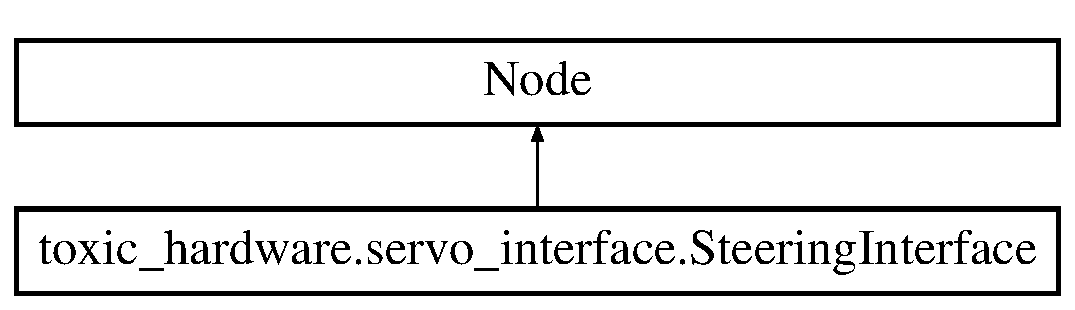
\includegraphics[height=2.000000cm]{dc/d0c/classtoxic__hardware_1_1servo__interface_1_1SteeringInterface}
\end{center}
\end{figure}
\doxysubsection*{Public Member Functions}
\begin{DoxyCompactItemize}
\item 
def \mbox{\hyperlink{classtoxic__hardware_1_1servo__interface_1_1SteeringInterface_ae64f0875afe3067b97ba370b354b9213}{\+\_\+\+\_\+init\+\_\+\+\_\+}} (self)
\item 
def \mbox{\hyperlink{classtoxic__hardware_1_1servo__interface_1_1SteeringInterface_a0762a6459eadaed0c4fad1263e369dbd}{steering\+\_\+callback}} (self, data)
\item 
def \mbox{\hyperlink{classtoxic__hardware_1_1servo__interface_1_1SteeringInterface_ae64f0875afe3067b97ba370b354b9213}{\+\_\+\+\_\+init\+\_\+\+\_\+}} (self)
\item 
def \mbox{\hyperlink{classtoxic__hardware_1_1servo__interface_1_1SteeringInterface_a0762a6459eadaed0c4fad1263e369dbd}{steering\+\_\+callback}} (self, data)
\end{DoxyCompactItemize}
\doxysubsection*{Public Attributes}
\begin{DoxyCompactItemize}
\item 
\mbox{\hyperlink{classtoxic__hardware_1_1servo__interface_1_1SteeringInterface_a4b0698733c4dfaffe8e2b4cd952b6f82}{subscription}}
\end{DoxyCompactItemize}


\doxysubsection{Constructor \& Destructor Documentation}
\mbox{\Hypertarget{classtoxic__hardware_1_1servo__interface_1_1SteeringInterface_ae64f0875afe3067b97ba370b354b9213}\label{classtoxic__hardware_1_1servo__interface_1_1SteeringInterface_ae64f0875afe3067b97ba370b354b9213}} 
\index{SteeringInterface@{SteeringInterface}!\_\_init\_\_@{\_\_init\_\_}}
\index{\_\_init\_\_@{\_\_init\_\_}!SteeringInterface@{SteeringInterface}}
\doxysubsubsection{\texorpdfstring{\_\_init\_\_()}{\_\_init\_\_()}\hspace{0.1cm}{\footnotesize\ttfamily [1/2]}}
{\footnotesize\ttfamily def \+\_\+\+\_\+init\+\_\+\+\_\+ (\begin{DoxyParamCaption}\item[{}]{self }\end{DoxyParamCaption})}


\begin{DoxyCode}{0}
\DoxyCodeLine{9     \textcolor{keyword}{def }\_\_init\_\_(self):}
\DoxyCodeLine{10         super().\_\_init\_\_(\textcolor{stringliteral}{'steering\_interface'})}
\DoxyCodeLine{11         self.subscription = self.create\_subscription(}
\DoxyCodeLine{12                 Float64,}
\DoxyCodeLine{13                 \textcolor{stringliteral}{'/steering'},}
\DoxyCodeLine{14                 self.steering\_callback,}
\DoxyCodeLine{15                 60}
\DoxyCodeLine{16                 )}
\DoxyCodeLine{17         self.subscription}
\DoxyCodeLine{18 }

\end{DoxyCode}
\mbox{\Hypertarget{classtoxic__hardware_1_1servo__interface_1_1SteeringInterface_ae64f0875afe3067b97ba370b354b9213}\label{classtoxic__hardware_1_1servo__interface_1_1SteeringInterface_ae64f0875afe3067b97ba370b354b9213}} 
\index{SteeringInterface@{SteeringInterface}!\_\_init\_\_@{\_\_init\_\_}}
\index{\_\_init\_\_@{\_\_init\_\_}!SteeringInterface@{SteeringInterface}}
\doxysubsubsection{\texorpdfstring{\_\_init\_\_()}{\_\_init\_\_()}\hspace{0.1cm}{\footnotesize\ttfamily [2/2]}}
{\footnotesize\ttfamily def \+\_\+\+\_\+init\+\_\+\+\_\+ (\begin{DoxyParamCaption}\item[{}]{self }\end{DoxyParamCaption})}


\begin{DoxyCode}{0}
\DoxyCodeLine{9     \textcolor{keyword}{def }\_\_init\_\_(self):}
\DoxyCodeLine{10         super().\_\_init\_\_(\textcolor{stringliteral}{'steering\_interface'})}
\DoxyCodeLine{11         self.subscription = self.create\_subscription(}
\DoxyCodeLine{12                 Float64,}
\DoxyCodeLine{13                 \textcolor{stringliteral}{'/steering'},}
\DoxyCodeLine{14                 self.steering\_callback,}
\DoxyCodeLine{15                 60}
\DoxyCodeLine{16                 )}
\DoxyCodeLine{17         self.subscription}
\DoxyCodeLine{18 }

\end{DoxyCode}


\doxysubsection{Member Function Documentation}
\mbox{\Hypertarget{classtoxic__hardware_1_1servo__interface_1_1SteeringInterface_a0762a6459eadaed0c4fad1263e369dbd}\label{classtoxic__hardware_1_1servo__interface_1_1SteeringInterface_a0762a6459eadaed0c4fad1263e369dbd}} 
\index{SteeringInterface@{SteeringInterface}!steering\_callback@{steering\_callback}}
\index{steering\_callback@{steering\_callback}!SteeringInterface@{SteeringInterface}}
\doxysubsubsection{\texorpdfstring{steering\_callback()}{steering\_callback()}\hspace{0.1cm}{\footnotesize\ttfamily [1/2]}}
{\footnotesize\ttfamily def steering\+\_\+callback (\begin{DoxyParamCaption}\item[{}]{self,  }\item[{}]{data }\end{DoxyParamCaption})}


\begin{DoxyCode}{0}
\DoxyCodeLine{19     \textcolor{keyword}{def }steering\_callback(self, data):}
\DoxyCodeLine{20         \textcolor{keyword}{global} servo\_pin}
\DoxyCodeLine{21         recived = data.data}
\DoxyCodeLine{22         \textcolor{keywordflow}{if} recived > 1:}
\DoxyCodeLine{23             recived = 1}
\DoxyCodeLine{24         \textcolor{keywordflow}{elif} recived < -\/1:}
\DoxyCodeLine{25             recived = -\/1}
\DoxyCodeLine{26         lgpio.tx\_pwm(}
\DoxyCodeLine{27                 servo\_pin,}
\DoxyCodeLine{28                 18,}
\DoxyCodeLine{29                 50,}
\DoxyCodeLine{30                 (7.2 + (recived*((10-\/5)/2)))}
\DoxyCodeLine{31                 )}
\DoxyCodeLine{32 }

\end{DoxyCode}
\mbox{\Hypertarget{classtoxic__hardware_1_1servo__interface_1_1SteeringInterface_a0762a6459eadaed0c4fad1263e369dbd}\label{classtoxic__hardware_1_1servo__interface_1_1SteeringInterface_a0762a6459eadaed0c4fad1263e369dbd}} 
\index{SteeringInterface@{SteeringInterface}!steering\_callback@{steering\_callback}}
\index{steering\_callback@{steering\_callback}!SteeringInterface@{SteeringInterface}}
\doxysubsubsection{\texorpdfstring{steering\_callback()}{steering\_callback()}\hspace{0.1cm}{\footnotesize\ttfamily [2/2]}}
{\footnotesize\ttfamily def steering\+\_\+callback (\begin{DoxyParamCaption}\item[{}]{self,  }\item[{}]{data }\end{DoxyParamCaption})}


\begin{DoxyCode}{0}
\DoxyCodeLine{19     \textcolor{keyword}{def }steering\_callback(self, data):}
\DoxyCodeLine{20         \textcolor{keyword}{global} servo\_pin}
\DoxyCodeLine{21         recived = data.data}
\DoxyCodeLine{22         \textcolor{keywordflow}{if} recived > 1:}
\DoxyCodeLine{23             recived = 1}
\DoxyCodeLine{24         \textcolor{keywordflow}{elif} recived < -\/1:}
\DoxyCodeLine{25             recived = -\/1}
\DoxyCodeLine{26         lgpio.tx\_pwm(}
\DoxyCodeLine{27                 servo\_pin,}
\DoxyCodeLine{28                 18,}
\DoxyCodeLine{29                 50,}
\DoxyCodeLine{30                 (7.2 + (recived*((10-\/5)/2)))}
\DoxyCodeLine{31                 )}
\DoxyCodeLine{32 }

\end{DoxyCode}


\doxysubsection{Member Data Documentation}
\mbox{\Hypertarget{classtoxic__hardware_1_1servo__interface_1_1SteeringInterface_a4b0698733c4dfaffe8e2b4cd952b6f82}\label{classtoxic__hardware_1_1servo__interface_1_1SteeringInterface_a4b0698733c4dfaffe8e2b4cd952b6f82}} 
\index{SteeringInterface@{SteeringInterface}!subscription@{subscription}}
\index{subscription@{subscription}!SteeringInterface@{SteeringInterface}}
\doxysubsubsection{\texorpdfstring{subscription}{subscription}}
{\footnotesize\ttfamily subscription}



The documentation for this class was generated from the following file\+:\begin{DoxyCompactItemize}
\item 
main\+\_\+ws/build/toxic\+\_\+hardware/build/lib/toxic\+\_\+hardware/\mbox{\hyperlink{build_2toxic__hardware_2build_2lib_2toxic__hardware_2servo__interface_8py}{servo\+\_\+interface.\+py}}\end{DoxyCompactItemize}

\chapter{File Documentation}
\hypertarget{toxic__hardware_2setup_8py}{}\doxysection{main\+\_\+ws/src/toxic\+\_\+hardware/setup.py File Reference}
\label{toxic__hardware_2setup_8py}\index{main\_ws/src/toxic\_hardware/setup.py@{main\_ws/src/toxic\_hardware/setup.py}}
\doxysubsection*{Namespaces}
\begin{DoxyCompactItemize}
\item 
 \mbox{\hyperlink{namespacesetup}{setup}}
\end{DoxyCompactItemize}
\doxysubsection*{Variables}
\begin{DoxyCompactItemize}
\item 
string \mbox{\hyperlink{namespacesetup_ad184fbcf6c2a41dfeaea25210baf1d7b}{package\+\_\+name}} = \textquotesingle{}toxic\+\_\+hardware\textquotesingle{}
\item 
\mbox{\hyperlink{namespacesetup_ab74e6bf80237ddc4109968cedc58c151}{name}}
\item 
\mbox{\hyperlink{namespacesetup_a4c7a521b8f1a0769c09bfa4a1fca7dab}{version}}
\item 
\mbox{\hyperlink{namespacesetup_a5191bfd75a28371588f75471591d5500}{packages}}
\item 
\mbox{\hyperlink{namespacesetup_ab2a4f143e926c57a50df01bb182a4fd5}{data\+\_\+files}}
\item 
\mbox{\hyperlink{namespacesetup_a047d4e9f7b152e767f7bd459218fe1fd}{install\+\_\+requires}}
\item 
\mbox{\hyperlink{namespacesetup_a270a33302dcfe1b60738df9ebbfb2103}{zip\+\_\+safe}}
\item 
\mbox{\hyperlink{namespacesetup_aed90451693186afcd612a6e3422085c9}{maintainer}}
\item 
\mbox{\hyperlink{namespacesetup_a3fc04e51dfecacd97621c848af907697}{maintainer\+\_\+email}}
\item 
\mbox{\hyperlink{namespacesetup_a2661f439a4a94ffdcd5e47ae1da0bb1d}{description}}
\item 
\mbox{\hyperlink{namespacesetup_a4e659be027e258b72df12349200a263e}{license}}
\item 
\mbox{\hyperlink{namespacesetup_a04f3a03d8b124a11d2008f990fb6335d}{tests\+\_\+require}}
\item 
\mbox{\hyperlink{namespacesetup_a0afb2eb153236846e2dd516c55a0e0dd}{entry\+\_\+points}}
\end{DoxyCompactItemize}

\hypertarget{toxic__vision_2setup_8py}{}\section{main\+\_\+ws/src/toxic\+\_\+vision/setup.py File Reference}
\label{toxic__vision_2setup_8py}\index{main\+\_\+ws/src/toxic\+\_\+vision/setup.\+py@{main\+\_\+ws/src/toxic\+\_\+vision/setup.\+py}}
\subsection*{Namespaces}
\begin{DoxyCompactItemize}
\item 
 \mbox{\hyperlink{namespacesetup}{setup}}
\end{DoxyCompactItemize}

\hypertarget{blinkers__interface_8py}{}\section{main\+\_\+ws/src/toxic\+\_\+hardware/toxic\+\_\+hardware/blinkers\+\_\+interface.py File Reference}
\label{blinkers__interface_8py}\index{main\+\_\+ws/src/toxic\+\_\+hardware/toxic\+\_\+hardware/blinkers\+\_\+interface.\+py@{main\+\_\+ws/src/toxic\+\_\+hardware/toxic\+\_\+hardware/blinkers\+\_\+interface.\+py}}
\subsection*{Classes}
\begin{DoxyCompactItemize}
\item 
class \mbox{\hyperlink{classtoxic__hardware_1_1blinkers__interface_1_1BlinkersInterface}{Blinkers\+Interface}}
\end{DoxyCompactItemize}
\subsection*{Namespaces}
\begin{DoxyCompactItemize}
\item 
 \mbox{\hyperlink{namespacetoxic__hardware_1_1blinkers__interface}{toxic\+\_\+hardware.\+blinkers\+\_\+interface}}
\end{DoxyCompactItemize}
\subsection*{Functions}
\begin{DoxyCompactItemize}
\item 
def \mbox{\hyperlink{namespacetoxic__hardware_1_1blinkers__interface_a205606096f1ce3bb8e412a407bee6b4b}{main}} (args=None)
\end{DoxyCompactItemize}
\subsection*{Variables}
\begin{DoxyCompactItemize}
\item 
\mbox{\hyperlink{namespacetoxic__hardware_1_1blinkers__interface_a6fd15ce64110e98b208bfe7a4ed33f52}{gpio\+\_\+pin}} = lgpio.\+gpiochip\+\_\+open(0)
\end{DoxyCompactItemize}

\hypertarget{controller_8py}{}\doxysection{main\+\_\+ws/src/toxic\+\_\+hardware/toxic\+\_\+hardware/controller.py File Reference}
\label{controller_8py}\index{main\_ws/src/toxic\_hardware/toxic\_hardware/controller.py@{main\_ws/src/toxic\_hardware/toxic\_hardware/controller.py}}
\doxysubsection*{Classes}
\begin{DoxyCompactItemize}
\item 
class \mbox{\hyperlink{classcontroller_1_1ControlSubscriber}{Control\+Subscriber}}
\end{DoxyCompactItemize}
\doxysubsection*{Namespaces}
\begin{DoxyCompactItemize}
\item 
 \mbox{\hyperlink{namespacecontroller}{controller}}
\end{DoxyCompactItemize}
\doxysubsection*{Functions}
\begin{DoxyCompactItemize}
\item 
def \mbox{\hyperlink{namespacecontroller_abe3b9157dce8796452422deae2a9161f}{main}} (args=None)
\end{DoxyCompactItemize}
\doxysubsection*{Variables}
\begin{DoxyCompactItemize}
\item 
\mbox{\hyperlink{namespacecontroller_ae6deea6e7d03b5d4db98ea209159e57f}{interface}} = lgpio.\+gpiochip\+\_\+open(0)
\item 
\mbox{\hyperlink{namespacecontroller_a257386444c3afd4030922ffb828f85fe}{roboclaw}} = Roboclaw(\char`\"{}/dev/tty\+ACM0\char`\"{}, 115200)
\end{DoxyCompactItemize}

\hypertarget{motor__interface_8py}{}\section{main\+\_\+ws/src/toxic\+\_\+hardware/toxic\+\_\+hardware/motor\+\_\+interface.py File Reference}
\label{motor__interface_8py}\index{main\+\_\+ws/src/toxic\+\_\+hardware/toxic\+\_\+hardware/motor\+\_\+interface.\+py@{main\+\_\+ws/src/toxic\+\_\+hardware/toxic\+\_\+hardware/motor\+\_\+interface.\+py}}
\subsection*{Classes}
\begin{DoxyCompactItemize}
\item 
class \mbox{\hyperlink{classtoxic__hardware_1_1motor__interface_1_1MotorInterface}{Motor\+Interface}}
\end{DoxyCompactItemize}
\subsection*{Namespaces}
\begin{DoxyCompactItemize}
\item 
 \mbox{\hyperlink{namespacetoxic__hardware_1_1motor__interface}{toxic\+\_\+hardware.\+motor\+\_\+interface}}
\end{DoxyCompactItemize}
\subsection*{Functions}
\begin{DoxyCompactItemize}
\item 
def \mbox{\hyperlink{namespacetoxic__hardware_1_1motor__interface_a2a214c16e0dd6e2551c72185d306001e}{main}} (args=None)
\end{DoxyCompactItemize}
\subsection*{Variables}
\begin{DoxyCompactItemize}
\item 
\mbox{\hyperlink{namespacetoxic__hardware_1_1motor__interface_a257386444c3afd4030922ffb828f85fe}{roboclaw}} = Roboclaw(\char`\"{}/dev/tty\+A\+C\+M0\char`\"{}, 115200)
\end{DoxyCompactItemize}

\hypertarget{oled__interface_8py}{}\section{main\+\_\+ws/src/toxic\+\_\+hardware/toxic\+\_\+hardware/oled\+\_\+interface.py File Reference}
\label{oled__interface_8py}\index{main\+\_\+ws/src/toxic\+\_\+hardware/toxic\+\_\+hardware/oled\+\_\+interface.\+py@{main\+\_\+ws/src/toxic\+\_\+hardware/toxic\+\_\+hardware/oled\+\_\+interface.\+py}}
\subsection*{Classes}
\begin{DoxyCompactItemize}
\item 
class \mbox{\hyperlink{classtoxic__hardware_1_1oled__interface_1_1OledInterface}{toxic\+\_\+hardware.\+oled\+\_\+interface.\+Oled\+Interface}}
\end{DoxyCompactItemize}
\subsection*{Namespaces}
\begin{DoxyCompactItemize}
\item 
 \mbox{\hyperlink{namespacetoxic__hardware_1_1oled__interface}{toxic\+\_\+hardware.\+oled\+\_\+interface}}
\end{DoxyCompactItemize}
\subsection*{Functions}
\begin{DoxyCompactItemize}
\item 
def \mbox{\hyperlink{namespacetoxic__hardware_1_1oled__interface_accb1149d5c8c645c307fcb16452ac121}{toxic\+\_\+hardware.\+oled\+\_\+interface.\+main}} (args=None)
\end{DoxyCompactItemize}
\subsection*{Variables}
\begin{DoxyCompactItemize}
\item 
\mbox{\hyperlink{namespacetoxic__hardware_1_1oled__interface_a863726b0bb3ebab40dfafb7dd98fd967}{toxic\+\_\+hardware.\+oled\+\_\+interface.\+R\+ST}} = None
\item 
int \mbox{\hyperlink{namespacetoxic__hardware_1_1oled__interface_adf756c0d3f22b55d2448ba7589ef6f60}{toxic\+\_\+hardware.\+oled\+\_\+interface.\+DC}} = 23
\item 
int \mbox{\hyperlink{namespacetoxic__hardware_1_1oled__interface_a828b6ed6d5ac147569b4e82a5e83135f}{toxic\+\_\+hardware.\+oled\+\_\+interface.\+S\+P\+I\+\_\+\+P\+O\+RT}} = 0
\item 
int \mbox{\hyperlink{namespacetoxic__hardware_1_1oled__interface_a9752681a2c24c6bba2ea3e38cf0731e5}{toxic\+\_\+hardware.\+oled\+\_\+interface.\+S\+P\+I\+\_\+\+D\+E\+V\+I\+CE}} = 0
\item 
\mbox{\hyperlink{namespacetoxic__hardware_1_1oled__interface_a79f95b96493be8450d34d9d1d12b6398}{toxic\+\_\+hardware.\+oled\+\_\+interface.\+disp}} = Adafruit\+\_\+\+S\+S\+D1306.\+S\+S\+D1306\+\_\+128\+\_\+64(rst=R\+ST)
\item 
\mbox{\hyperlink{namespacetoxic__hardware_1_1oled__interface_a4a60f1ea9d94d7defd7e96d957f6d35d}{toxic\+\_\+hardware.\+oled\+\_\+interface.\+width}} = disp.\+width
\item 
\mbox{\hyperlink{namespacetoxic__hardware_1_1oled__interface_a04ce862db440b383129c968ecb0651c6}{toxic\+\_\+hardware.\+oled\+\_\+interface.\+height}} = disp.\+height
\item 
\mbox{\hyperlink{namespacetoxic__hardware_1_1oled__interface_adaad3157e9032049ecca2c4ee24cfdb8}{toxic\+\_\+hardware.\+oled\+\_\+interface.\+image}} = Image.\+new(\textquotesingle{}1\textquotesingle{}, (width, height))
\item 
\mbox{\hyperlink{namespacetoxic__hardware_1_1oled__interface_a6b3585c5a31faea000d6630399894c0c}{toxic\+\_\+hardware.\+oled\+\_\+interface.\+draw}} = Image\+Draw.\+Draw(image)
\item 
\mbox{\hyperlink{namespacetoxic__hardware_1_1oled__interface_aaeac32a54a5c8dbb7b165484dd3ff515}{toxic\+\_\+hardware.\+oled\+\_\+interface.\+outline}}
\item 
\mbox{\hyperlink{namespacetoxic__hardware_1_1oled__interface_a6249580750b8516240d739a5bd55a3c6}{toxic\+\_\+hardware.\+oled\+\_\+interface.\+fill}}
\item 
int \mbox{\hyperlink{namespacetoxic__hardware_1_1oled__interface_a551f91b346cdc03bdfdb32a7a71da5d4}{toxic\+\_\+hardware.\+oled\+\_\+interface.\+padding}} = -\/2
\item 
int \mbox{\hyperlink{namespacetoxic__hardware_1_1oled__interface_a08522c6a4a076052b31d7123c3131119}{toxic\+\_\+hardware.\+oled\+\_\+interface.\+top}} = padding
\item 
int \mbox{\hyperlink{namespacetoxic__hardware_1_1oled__interface_a046619703df951ada8a9a00b438a983c}{toxic\+\_\+hardware.\+oled\+\_\+interface.\+bottom}} = height-\/padding
\item 
int \mbox{\hyperlink{namespacetoxic__hardware_1_1oled__interface_a011bb65915d0847fe86e5dfafef6536d}{toxic\+\_\+hardware.\+oled\+\_\+interface.\+x}} = 0
\item 
\mbox{\hyperlink{namespacetoxic__hardware_1_1oled__interface_a884f1d5a8f04b13797b90ef2007ba2b7}{toxic\+\_\+hardware.\+oled\+\_\+interface.\+font}} = Image\+Font.\+load\+\_\+default()
\end{DoxyCompactItemize}

\hypertarget{roboclaw__3_8py}{}\section{main\+\_\+ws/src/toxic\+\_\+hardware/toxic\+\_\+hardware/roboclaw\+\_\+3.py File Reference}
\label{roboclaw__3_8py}\index{main\+\_\+ws/src/toxic\+\_\+hardware/toxic\+\_\+hardware/roboclaw\+\_\+3.\+py@{main\+\_\+ws/src/toxic\+\_\+hardware/toxic\+\_\+hardware/roboclaw\+\_\+3.\+py}}
\subsection*{Classes}
\begin{DoxyCompactItemize}
\item 
class \mbox{\hyperlink{classtoxic__hardware_1_1roboclaw__3_1_1Roboclaw}{Roboclaw}}
\item 
class \mbox{\hyperlink{classtoxic__hardware_1_1roboclaw__3_1_1Roboclaw_1_1Cmd}{Roboclaw.\+Cmd}}
\end{DoxyCompactItemize}
\subsection*{Namespaces}
\begin{DoxyCompactItemize}
\item 
 \mbox{\hyperlink{namespacetoxic__hardware_1_1roboclaw__3}{toxic\+\_\+hardware.\+roboclaw\+\_\+3}}
\end{DoxyCompactItemize}

\hypertarget{servo__interface_8py}{}\section{main\+\_\+ws/src/toxic\+\_\+hardware/toxic\+\_\+hardware/servo\+\_\+interface.py File Reference}
\label{servo__interface_8py}\index{main\+\_\+ws/src/toxic\+\_\+hardware/toxic\+\_\+hardware/servo\+\_\+interface.\+py@{main\+\_\+ws/src/toxic\+\_\+hardware/toxic\+\_\+hardware/servo\+\_\+interface.\+py}}
\subsection*{Classes}
\begin{DoxyCompactItemize}
\item 
class \mbox{\hyperlink{classtoxic__hardware_1_1servo__interface_1_1SteeringInterface}{toxic\+\_\+hardware.\+servo\+\_\+interface.\+Steering\+Interface}}
\end{DoxyCompactItemize}
\subsection*{Namespaces}
\begin{DoxyCompactItemize}
\item 
 \mbox{\hyperlink{namespacetoxic__hardware_1_1servo__interface}{toxic\+\_\+hardware.\+servo\+\_\+interface}}
\end{DoxyCompactItemize}
\subsection*{Functions}
\begin{DoxyCompactItemize}
\item 
def \mbox{\hyperlink{namespacetoxic__hardware_1_1servo__interface_a2278d6779516e4e6c64047946e8e9595}{toxic\+\_\+hardware.\+servo\+\_\+interface.\+main}} (args=None)
\end{DoxyCompactItemize}
\subsection*{Variables}
\begin{DoxyCompactItemize}
\item 
\mbox{\hyperlink{namespacetoxic__hardware_1_1servo__interface_a62a4569a9213571f92544a77c5e49228}{toxic\+\_\+hardware.\+servo\+\_\+interface.\+servo\+\_\+pin}} = lgpio.\+gpiochip\+\_\+open(0)
\end{DoxyCompactItemize}

\hypertarget{lane__detector_8py}{}\section{main\+\_\+ws/src/toxic\+\_\+vision/toxic\+\_\+vision/lane\+\_\+detector.py File Reference}
\label{lane__detector_8py}\index{main\+\_\+ws/src/toxic\+\_\+vision/toxic\+\_\+vision/lane\+\_\+detector.\+py@{main\+\_\+ws/src/toxic\+\_\+vision/toxic\+\_\+vision/lane\+\_\+detector.\+py}}
\subsection*{Classes}
\begin{DoxyCompactItemize}
\item 
class \mbox{\hyperlink{classtoxic__vision_1_1lane__detector_1_1ImageSubscriber}{toxic\+\_\+vision.\+lane\+\_\+detector.\+Image\+Subscriber}}
\end{DoxyCompactItemize}
\subsection*{Namespaces}
\begin{DoxyCompactItemize}
\item 
 \mbox{\hyperlink{namespacetoxic__vision_1_1lane__detector}{toxic\+\_\+vision.\+lane\+\_\+detector}}
\end{DoxyCompactItemize}
\subsection*{Functions}
\begin{DoxyCompactItemize}
\item 
def \mbox{\hyperlink{namespacetoxic__vision_1_1lane__detector_ae3bdbfab97718df7c906f65d19f10dfd}{toxic\+\_\+vision.\+lane\+\_\+detector.\+to\+\_\+normal\+\_\+form}} (x1, y1, x2, y2)
\item 
def \mbox{\hyperlink{namespacetoxic__vision_1_1lane__detector_a365ec8dd4fef50dc9623183b3e39e22d}{toxic\+\_\+vision.\+lane\+\_\+detector.\+mouse\+\_\+callback}} (event, x, y, flags, param)
\item 
def \mbox{\hyperlink{namespacetoxic__vision_1_1lane__detector_a7a56502e886845d86ce39e37d087b5a8}{toxic\+\_\+vision.\+lane\+\_\+detector.\+main}} (args=None)
\end{DoxyCompactItemize}
\subsection*{Variables}
\begin{DoxyCompactItemize}
\item 
list \mbox{\hyperlink{namespacetoxic__vision_1_1lane__detector_aa1b547c10a2da901b93727a9e2d069be}{toxic\+\_\+vision.\+lane\+\_\+detector.\+upper\+\_\+color}} = \mbox{[}130, 254, 255\mbox{]}
\item 
list \mbox{\hyperlink{namespacetoxic__vision_1_1lane__detector_afb4d5c2eb4ff5c30128774f99941786a}{toxic\+\_\+vision.\+lane\+\_\+detector.\+lower\+\_\+color}} = \mbox{[}0, 216, 0\mbox{]}
\item 
float \mbox{\hyperlink{namespacetoxic__vision_1_1lane__detector_ac799a869f5eb8830039f61fb626fc82a}{toxic\+\_\+vision.\+lane\+\_\+detector.\+left\+\_\+min}} = 0.\+7
\item 
int \mbox{\hyperlink{namespacetoxic__vision_1_1lane__detector_addb36fd74f99c2788d7e153c8bf15de6}{toxic\+\_\+vision.\+lane\+\_\+detector.\+left\+\_\+max}} = 1
\item 
float \mbox{\hyperlink{namespacetoxic__vision_1_1lane__detector_a1d19d5688abe600bc56eea89a9037084}{toxic\+\_\+vision.\+lane\+\_\+detector.\+right\+\_\+min}} = -\/1.\+0
\item 
float \mbox{\hyperlink{namespacetoxic__vision_1_1lane__detector_ad4a23b932ce65760f65729e50a2bdd7d}{toxic\+\_\+vision.\+lane\+\_\+detector.\+right\+\_\+max}} = -\/0.\+7
\item 
float \mbox{\hyperlink{namespacetoxic__vision_1_1lane__detector_a9b66066e6cda0deea6ece92c0f567c12}{toxic\+\_\+vision.\+lane\+\_\+detector.\+variance}} = 0.\+1
\item 
int \mbox{\hyperlink{namespacetoxic__vision_1_1lane__detector_a1829d358a957df5a0df24568e68ccc81}{toxic\+\_\+vision.\+lane\+\_\+detector.\+delta}} = 5
\item 
int \mbox{\hyperlink{namespacetoxic__vision_1_1lane__detector_a0b6ffdfa9cdd7fc0dc9fbcf093f7be85}{toxic\+\_\+vision.\+lane\+\_\+detector.\+upper}} = -\/1
\item 
int \mbox{\hyperlink{namespacetoxic__vision_1_1lane__detector_ae6e94ffeaf31d2adbfbd7d3919ed7f75}{toxic\+\_\+vision.\+lane\+\_\+detector.\+lower}} = 1000
\item 
int \mbox{\hyperlink{namespacetoxic__vision_1_1lane__detector_af1171665614ff59f09a4fdb7505f145c}{toxic\+\_\+vision.\+lane\+\_\+detector.\+lefter}} = 1000
\item 
int \mbox{\hyperlink{namespacetoxic__vision_1_1lane__detector_a2eaabc57b6e097c84cb0ab370d95b65e}{toxic\+\_\+vision.\+lane\+\_\+detector.\+righter}} = -\/1
\item 
list \mbox{\hyperlink{namespacetoxic__vision_1_1lane__detector_a13998232e16bd76d1da86f068ac01230}{toxic\+\_\+vision.\+lane\+\_\+detector.\+frame}} = \mbox{[}$\,$\mbox{]}
\end{DoxyCompactItemize}

\hypertarget{webcam__pub_8py}{}\section{main\+\_\+ws/src/toxic\+\_\+vision/toxic\+\_\+vision/webcam\+\_\+pub.py File Reference}
\label{webcam__pub_8py}\index{main\+\_\+ws/src/toxic\+\_\+vision/toxic\+\_\+vision/webcam\+\_\+pub.\+py@{main\+\_\+ws/src/toxic\+\_\+vision/toxic\+\_\+vision/webcam\+\_\+pub.\+py}}
\subsection*{Classes}
\begin{DoxyCompactItemize}
\item 
class \mbox{\hyperlink{classtoxic__vision_1_1webcam__pub_1_1ImagePublisher}{toxic\+\_\+vision.\+webcam\+\_\+pub.\+Image\+Publisher}}
\end{DoxyCompactItemize}
\subsection*{Namespaces}
\begin{DoxyCompactItemize}
\item 
 \mbox{\hyperlink{namespacetoxic__vision_1_1webcam__pub}{toxic\+\_\+vision.\+webcam\+\_\+pub}}
\end{DoxyCompactItemize}
\subsection*{Functions}
\begin{DoxyCompactItemize}
\item 
def \mbox{\hyperlink{namespacetoxic__vision_1_1webcam__pub_a0d57aeae4d44f1dcb33eed5082cf3c87}{toxic\+\_\+vision.\+webcam\+\_\+pub.\+main}} (args=None)
\end{DoxyCompactItemize}

\hypertarget{webcam__sub_8py}{}\doxysection{main\+\_\+ws/src/toxic\+\_\+vision/toxic\+\_\+vision/webcam\+\_\+sub.py File Reference}
\label{webcam__sub_8py}\index{main\_ws/src/toxic\_vision/toxic\_vision/webcam\_sub.py@{main\_ws/src/toxic\_vision/toxic\_vision/webcam\_sub.py}}


Very simple image subscriber to /raw\+\_\+rgb node.  


\doxysubsection*{Classes}
\begin{DoxyCompactItemize}
\item 
class \mbox{\hyperlink{classwebcam__sub_1_1ImageSubscriber}{Image\+Subscriber}}
\end{DoxyCompactItemize}
\doxysubsection*{Namespaces}
\begin{DoxyCompactItemize}
\item 
 \mbox{\hyperlink{namespacewebcam__sub}{webcam\+\_\+sub}}
\end{DoxyCompactItemize}
\doxysubsection*{Functions}
\begin{DoxyCompactItemize}
\item 
def \mbox{\hyperlink{namespacewebcam__sub_a17962900f744f2e667d37e9568cc5ea2}{main}} (args=None)
\begin{DoxyCompactList}\small\item\em This function create the subscriber and execute it. \end{DoxyCompactList}\end{DoxyCompactItemize}


\doxysubsection{Detailed Description}
Very simple image subscriber to /raw\+\_\+rgb node. 

\hypertarget{webcam__sub_8py_detailed_webcam_pub}{}\doxysubsection{Detail}\label{webcam__sub_8py_detailed_webcam_pub}
This script create an image subscriber to \char`\"{}/raw\+\_\+rgb\char`\"{} and draw the recived frame, this node\textquotesingle{}s used just as test to verify the image publisher and nodes communication performance.\hypertarget{webcam__sub_8py_parameters_webcam_subscriber}{}\doxysubsection{Important parameters to change.}\label{webcam__sub_8py_parameters_webcam_subscriber}
On this code, you don\textquotesingle{}r need to change anything, except if you\textquotesingle{}ve changed the name of the image publisher node, or just wanna check another node.\hypertarget{webcam__sub_8py_dependences_webcam_sub}{}\doxysubsection{Dependences.}\label{webcam__sub_8py_dependences_webcam_sub}

\begin{DoxyItemize}
\item rclpy
\begin{DoxyItemize}
\item Used to node manipulation.
\end{DoxyItemize}
\item rclpy.\+node
\begin{DoxyItemize}
\item Used to node manipulation. (really idk why we don\textquotesingle{}t import only this or the above library)
\end{DoxyItemize}
\item sensor\+\_\+msgs.\+msg.\+Image
\begin{DoxyItemize}
\item Used to be able to use the Image message type (very self-\/explained, I think)
\end{DoxyItemize}
\item cv\+Bridge.\+cv\+Bridge
\begin{DoxyItemize}
\item Used to parse a ROS2\textquotesingle{}s Image type to Open\+Cv Frame type
\end{DoxyItemize}
\item cv2
\begin{DoxyItemize}
\item In this case it\textquotesingle{}s just used to draw the image in a frame.
\end{DoxyItemize}
\end{DoxyItemize}\hypertarget{webcam__sub_8py_rights_webcam_Sub}{}\doxysubsection{Copyright}\label{webcam__sub_8py_rights_webcam_Sub}
This script conforms part from \textquotesingle{}El tóxico\textquotesingle{} and it\textquotesingle{}s licenced unser GPL 3V0.\hypertarget{webcam__sub_8py_code_webcam_subscriber}{}\doxysubsection{Code Spinnet.}\label{webcam__sub_8py_code_webcam_subscriber}

\begin{DoxyCodeInclude}{0}

\end{DoxyCodeInclude}
 
\hypertarget{README_8md}{}\section{R\+E\+A\+D\+M\+E.\+md File Reference}
\label{README_8md}\index{R\+E\+A\+D\+M\+E.\+md@{R\+E\+A\+D\+M\+E.\+md}}

%--- End generated contents ---

% Index
\backmatter
\newpage
\phantomsection
\clearemptydoublepage
\addcontentsline{toc}{chapter}{Index}
\printindex

\end{document}
